
\chapter{Динамічні акусто--індуковані ефекти в радіаційно опромінених та неопромінених кремнієвих структурах з p--n переходом\label{Ch_SSC}}


\section{Особливості використання активного ультразвуку}
Значна частина представлених у дисертаційній роботі результатів (розділи~\ref{Ch_SSC}, \ref{Ch_GammaSD}, \ref{Ch_USL_T_SD} та \ref{Ch_UST_MW}) пов'язана з дослідженням ефектів, які відбуваються в напівпровідникових структурах внаслідок
поширення в них акустичних хвиль (АХ) мегагерцевого діапазону.
У зв'язку з тим, що використання ультразвуку (УЗ), на жаль, ще не є стандартним способом впливу на напівпровідникові кристали,
у цьому параграфі представлено узагальнена  інформація щодо відповідних експериментальних методик.

Зокрема, представлені описи процедур ультразвукової обробки (УЗО) та ультразвукового навантаження (УЗН).
Відмінності у використанні цих термінів пов'язані з оборотністю АІ процесів.
Так, в першому випадку (УЗО), внаслідок поширення пружних хвиль відбуваються незворотні (залишкові) зміни властивостей напівпровідникових структур.
Тоді як в другому випадку (УЗН), ефекти є оборотніми (динамічними), зміни електрофізичних параметрів спостерігаються лише за умов поширення АХ;
після припинення дії УЗ параметри поступово повертаються до своїх вихідних (до початку УЗН) значень.

Для збудження УЗ у досліджуваних структурах використовувалися п'єзоелектричні перетворювачі,
виготовлені з пластин ніобату літію (LiNbO$_3$) з металізацією обох граней шляхом вакуумного напилення алюмінію.
Для збудження повздовжніх та поперечних акустичних хвиль використовувалися пластини зі зрізами $(Y\!+\!36^\circ)$ та $(Y\!+\!163^\circ)$, відповідно.

З літератури \cite{Ostapenko1995,Davletova2008,Davletova2009,Pashaev2014r} відомо, що АХ з частотою, що знаходиться в діапазоні $1\div30$~МГц, здатні впливати на стан дефектів у кремнії.
Саме такий частотний діапазон був використаний у дослідженнях, результати яких представлені далі.
В експериментах проводилось збудження УЗ з частотою $f_\mathtt{US}$, яка знаходилась поблизу першої або третьої гармоніки товщинного резонансу пластинки.
Значення резонансної частоти перетворювачів визначалось за допомогою приладу для дослідження АЧХ Х1--38.
Безпосереднє значення $f_\mathtt{US}$, при якому введення пружних коливань у зразок відбувається найбільш ефективно, визначалось стандартним методом за максимальною амплітудою коливань краплі води (або вакуумного масла), розміщеної на поверхні перетворювача, при прикладанні до його граней змінної напруги.

Попередні дослідження різних авторів \cite{Davletova2008,Davletova2009,Pashaev2014r,Vlasov2009r} показали, що використання УЗ
з інтенсивністю, як правило, $W_\mathtt{US}\geq3$~Вт/см$^2$ спричинює необоротні (залишкові) зміни властивостей кремнієвих структур.
Ці процеси можуть бути пов'язані з відпалом радіаційних дефектів, формуванням нових дефектів або переміщенням вже існуючих, на відстані, що значно перевищують міжатомну відстань.
Так як метою частини роботи (розділи~\ref{Ch_SSC}, \ref{Ch_GammaSD} та \ref{Ch_USL_T_SD}) було дослідження саме оборотних АІ ефектів,
то переважна більшість УЗН проводилась при $W_\mathtt{US} \leq 1$~Вт/см$^2$.
Детальніше процедура оцінки $W_\mathtt{US}$ та інших параметрів УЗ впливу наведена у параграфах \ref{SC:USL} та \ref{SSDB:USL}.

Для того, щоб під час УЗН позбавитися впливу п'єзоелектричного поля, яке супроводжує механічні коливання пластини LiNbO$_3$,  як на параметри напівпровідникових структур, так і на процес вимірювання електрофізичних параметрів,
перетворювач екранувався.
Як наслідок, можна стверджувати, що виявлені під час УЗН ефекти визначаються лише знакозмінною деформацією.
Для створення акустичного контакту при різних УЗН використовувалися вакуумне масло, клей БФ6, піцеїн.
Детальні схеми акустичного навантаження зразків наведено у кожному розділі.


Структури, в яких проводилися дослідження ефектів УЗН, містили енергетичний бар'єр, пов'язаний з наявністю контакту МН або $p-n$ переходу, розміщений поблизу однієї з поверхонь зразка.
Введення УЗ відбувалось з боку грані, протилежної до місця розташування бар'єру.
Тобто, напрям поширення АХ перпендикулярний площині бар'єру і збігається з напрямом струму, який виникає під час прикладення до структури електричної напруги (або при освітленні, якщо об'єктом дослідження є сонячний елемент).
При цьому, при використанні повздовжніх хвиль вимушені зміщення атомів відбуваються у тому самому напрямі, тоді як для поперечних хвиль коливання частинок спрямовані перпендикулярно до електричного струму у площині бар'єру.

Раніше показано \cite{Ostapenko1995,YOlikhTPL2011,Ostrovskii2001}, що характерний час зміни властивостей кремнієвих структур під дією УЗ не перевищує $2\cdot10^3$~c.
Для того, щоб дочекатися закінчення всіх перехідних АІ процесів, використовувалася наступна експериментально процедура.
УЗН починалося при кімнатній температурі.
Після цього зразки перебували не менше 60~хв за умов поширення в них пружних коливань і лише після цього, не припиняючи дії УЗ, починалися вимірювання електрофізичних параметрів та/або процеси нагріву або охолодження.

Відомо, що під час навантаження п'єзоелектричний перетворювач нагрівається.
Температура структур, які досліджувалися, контролювалася диференційною термопарою мідь--константан.
В роботі проводилось порівняння значень параметрів, отриманих за однакових температур в умовах УЗН зразків та без нього.
Це дозволяло виокремити АІ зміни характеристик напівпровідникових структур, від змін, пов'язаних з їх розігрівом під час УЗН.
Для оцінки величини впливу УЗ на певний параметр $P$ (яким могла бути напруга холостого ходу, фактор неідеальності, величина зворотного струму тощо),
використовувалися його абсолютні
 \begin{equation}
 \label{eqAbsDelta}
\Delta P=P_{in}-P_\mathtt{US}
 \end{equation}
чи відносні зміни
 \begin{equation}
 \label{eqEpsDelta}
\varepsilon_P=\frac{P_{in}-P_\mathtt{US}}{P_{in}},
 \end{equation}
де нижні індекси <<$\mathtt{US}$>> та <<$in$>> вказують на те, що відповідне значення параметра було отримане при однаковій температурі за умов УЗН та без нього, відповідно.

При УЗО процеси впливу АХ та вимірювання параметрів були розділені в часу і тому нагальної необхідності екранування п'єзоелектричних полів не було.
Як наслідок, експериментальна схема простіша, п'єзоперетворювач безпосередньо акустично контактував з досліджуваною структурою.




\section{Структура кремнієвих сонячних елементів та режими їх радіаційного опромінення\label{SSC}}
Сонячні елементи, які досліджувалися в роботі, були створені на основі пластин кремнію діаметром близько 100~мм.
Пластини  товщиною 300~мкм з орієнтацією (111) були вирізані зі злитків, вирощених за методом Чохральського.
Легування здійснювалось шляхом додавання у розплав атомів бору (кремній марки КДБ10).
У дослідженому температурному діапазоні концентрація основних носіїв заряду складала величину $p_p=1,4\cdot10^{15}$~см$^{-3}$.
% та $p_p=4.5\cdot10^{15}$~см$^{-3}$).

Для створення $n^+$ емітера проводилась імплантація іонів фосфору, після закінчення якої було проведено активізуючий відпал.
Як наслідок, був створений шар з електронною провідністю товщиною близько  0,5~мкм з концентрацією вільних носіїв заряду $10^{19}$~см$^{-3}$.

Поверхня пластини була пасивована шляхом нанесення плівки Al$_2$O$_3$.
Крім того, на фронтальну поверхню був нанесений антивідбиваючий шар діоксиду титану (TiO$_2$) з використанням методу APCVD (atmospheric pressure chemical  vapour  deposition).
З використанням методу трафаретного друку (screen printing) було створено омічні алюмінієві електроди (суцільний на задній поверхні та металева сітка на передній).
Нарешті, був проведений швидкий відпал отриманих структур при температурі $800^\circ$C тривалістю декілька хвилин.
Структура досліджених кремнієвих сонячних елементів (КСЕ) зображена на Рис.~\ref{figSSC},а.
Зауважимо, що цей рисунок наведено без збереження масштабних співвідношень між окремими частинами.

Для досліджень використовувалися зразки площею $1,5\div2,1$~cm$^{2}$, вирізані з різних (переважно центральних) областей пластини.
Для позначення зразків надалі використовується запис на кшталт SSC$x$, де $x$ --- номер зразка.
Місце розташування зразків на вихідній пластині показано на Рис.~\ref{figSSC},б.


\begin{figure}
\center
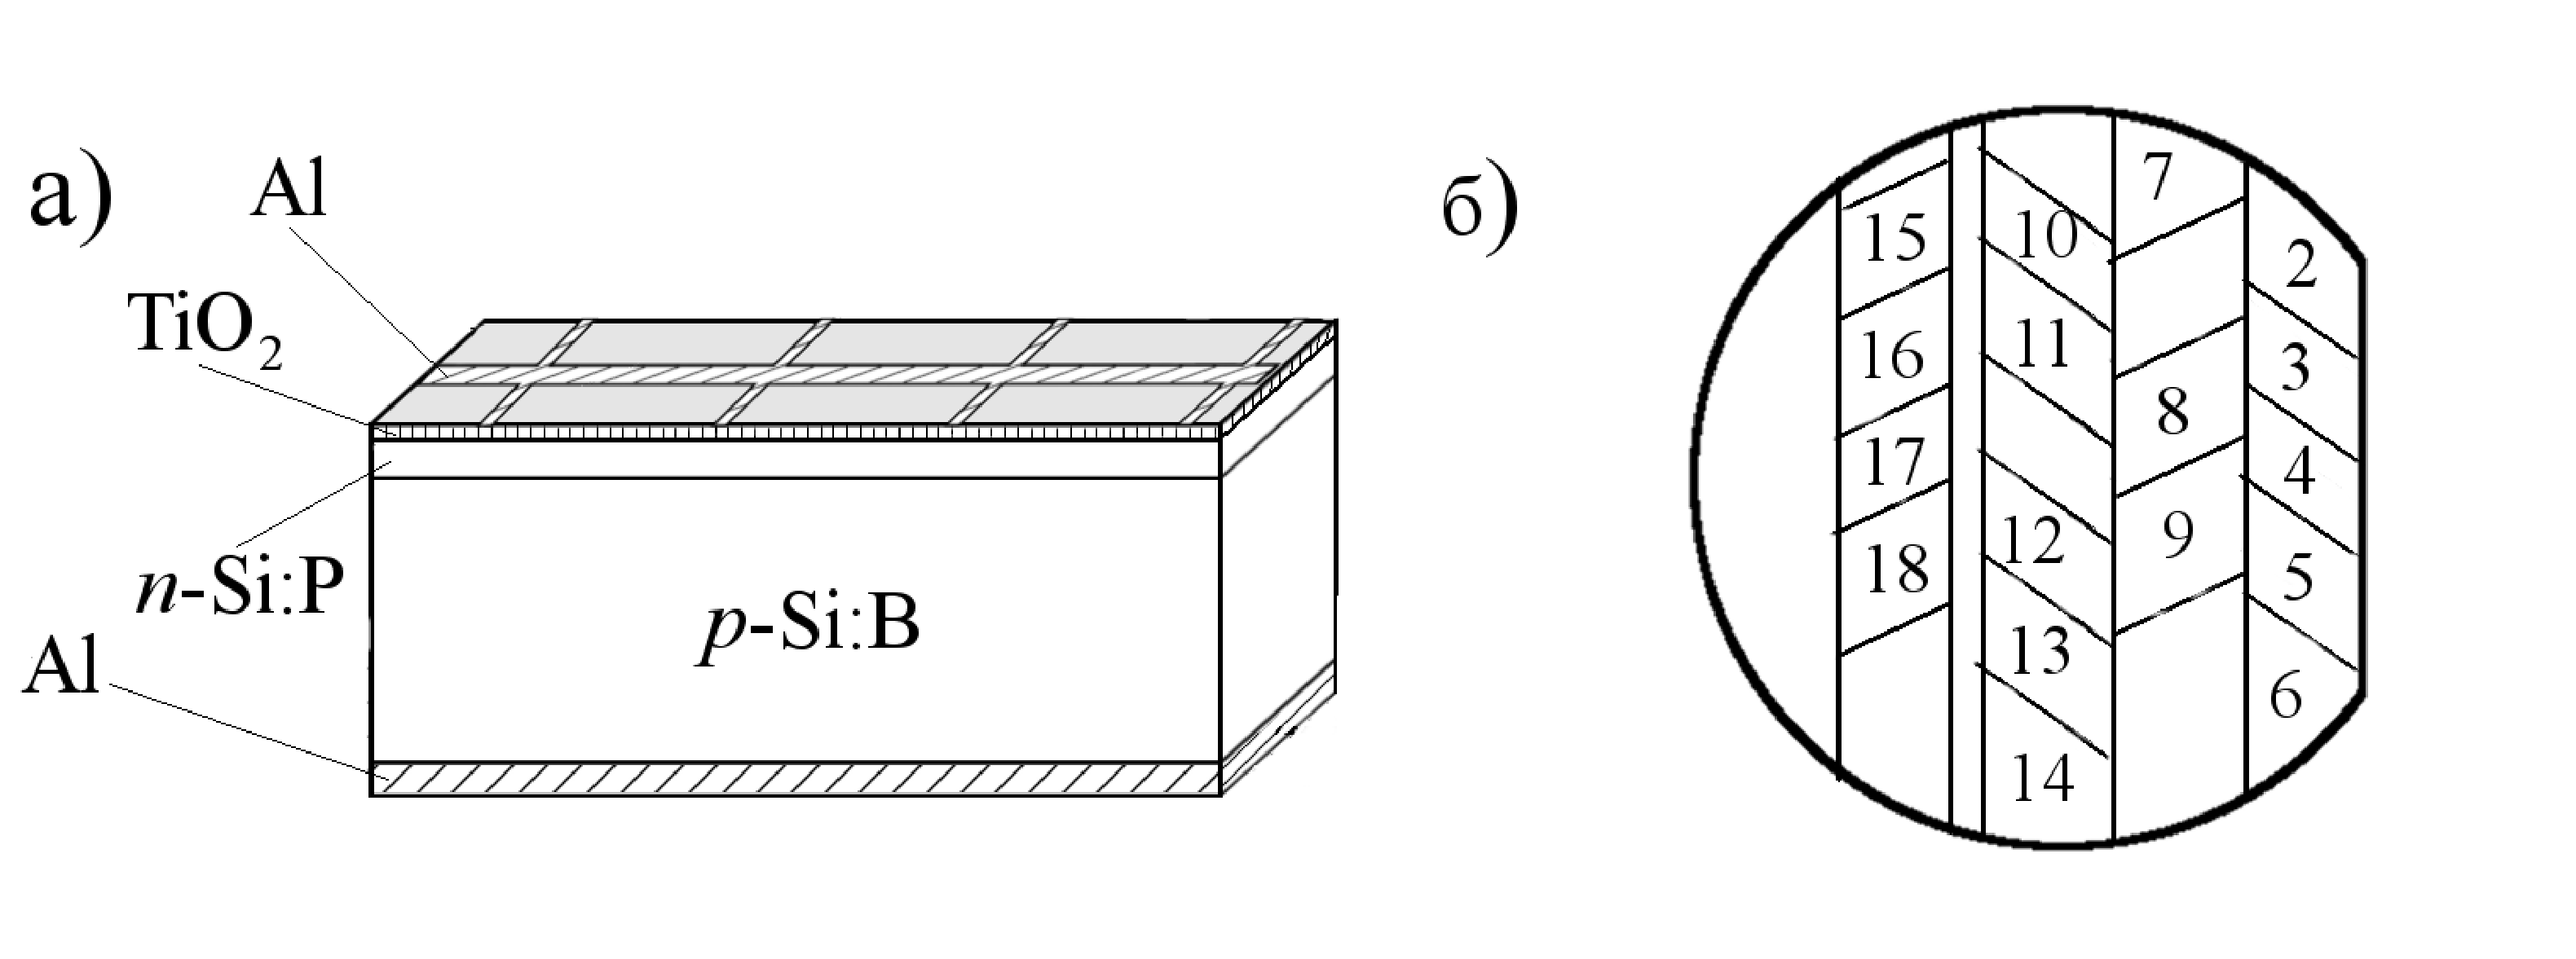
\includegraphics[width=1.0\textwidth]{SSC}%
\caption{\label{figSSC}
Структура кремнієвих сонячних елементів (а) та місце розташування зразків (б).
}
\end{figure}


\begin{table}[b]
\caption{\label{tabSSCSample}Параметри опромінених кремнієвих сонячних елементів.
}
\begin{tabular}{|c|c|c|c|c|c|}
%\begin{tabularx}{\textwidth}{|>{\centering\arraybackslash}X|
%                             >{\centering\arraybackslash}X|
%                            >{\centering\arraybackslash}X|
%                            >{\centering\arraybackslash}X|
%                            >{\centering\arraybackslash}X|
%                            >{\centering\arraybackslash}X|
%                            }
\hline
\multirow{2}{*}{Зразок} &Тип&$D$,&$\Psi$, &NIEL,& $D_d$,  \\
&опромінення& рад& см$^{-2}$&MеВ~см$^2$/г& MеВ/г \\
\hline
nSC4&нейтрони&4,5$\cdot$10$^3$&4$\cdot$10$^{11}$&2,04$\cdot$10$^{-3}$&8,2$\cdot$10$^{8}$\\ \hline
g6SC8&$\gamma$--$^{60}$Co&1$\cdot$10$^6$&1,6$\cdot$10$^{15}$&1,07$\cdot$10$^{-7}$\cite{NIEL:Akkerman}&$(1,7\div2,1)\cdot 10^{8}$\\
\cline{1-4}
\cline{6-6}
g7SC12&$\gamma$--$^{60}$Co&1$\cdot$10$^7$&1,6$\cdot$10$^{16}$&1,31$\cdot$10$^{-7}$\cite{NIEL:Messenger}&$(1,7\div2,1)\cdot 10^9$\\ \hline
\end{tabular}
%\end{tabularx}
\end{table}

Частина зразків, використаних для досліджень, була опромінена або реакторними нейтронами, або гамма--квантами $^{60}$Co.
Флюєнс $\Psi$ нейтронного опромінення складав $4\cdot10^{11}$~см$^{-2}$,
для позначення нейтронно опромінених зразків використовується префікс <<n>> (наприклад <<nSC4>>).
Доза $D$ опромінення гамма-квантами дорівнювала $10^6$ або $10^7$~рад, для позначення відповідних зразків використовуються префікси <<g6>> та <<g7>>, відповідно.

Значення доз та флюєнсів наведено в Таблиці~\ref{tabSSCSample}.
Для визначення кореляцій між $D$ та $\Psi$ для нейтронного та $\gamma-^{60}$Co опромінення використовувалися дані робіт \cite{NIEL:Akkerman,Brauning}.
У цій таблиці також наведено дані щодо величини NIEL (non--ionizing energy losses, енергетичні втрати, не пов'язані з іонізацією) при поширенні нейтронів та гамма--квантів $^{60}$Co в кристалах кремнію.
NIEL характеризує втрати енергії налітаючої частинки на одиницю довжини шляху, пов'язані зі зміщенням атомів ґратки \cite{NIEL:Huhtinen,NIEL:Messenger}, тобто, фактично, процеси радіаційного дефектоутворення.
Зокрема, вважається що радіаційне ушкодження кристалів характеризується такою величиною, як $D_d=\Psi\cdot \mbox{NIEL}$ (displacement damage dose) \cite{NIEL:Messenger}.
Величини $D_d$ для досліджених структур також розміщені у Таблиці~\ref{tabSSCSample}.
З наведених даних видно, що як при використанні нейтронів, так і $\gamma$--квантів очікуване пошкодження кристалічної структури є близьким.
Проте, як відомо,  опромінення різного типу викликає появу різних за структурою дефектів.
Зокрема, $\gamma$--промені викликають появу, переважно, А--центрів \cite{NIEL:Jafari,Gamma:Prabhakara,NIEL:Moll}, тоді як нейтрони призводять до появи вакансійних кластерів\cite{Rew:Srour,Junkes}, областей розупорядкування  \cite{Neutron:Arutyunov} та комплексів C$_i$O$_i$ \cite{NIEL:Moll,neutron:Londos}.
Більш детально це питання розглянуте у розділі~\ref{Rad_SSC}.

Відомо \cite{RadBook}, що після радіаційного опромінення, особливо нейтронного, \cite{NIEL:Moll,Rew:Srour} у кристалах кремнію відбуваються довготривалі перехідні процеси, пов'язані з утворенням вторинних радіаційних дефектів (РД).
Для того, щоб уникнути впливу подібних процесів зразки після опромінення перед початком досліджень, результати який наведено далі, зберігались протягом п'яти років при кімнатній температурі.




\section{Режими ультразвукового навантаження кристалічних кремнієвих сонячних елементів\label{SC:USL}}
Схема акустичного навантаження зразків наведено на Рис.~\ref{figUSL:SC}.
Акустичний контакт створювався за допомогою вакуумного масла при використанні повздовжніх хвиль та клею БФ6 --- для поперечних.

\begin{figure}
\center
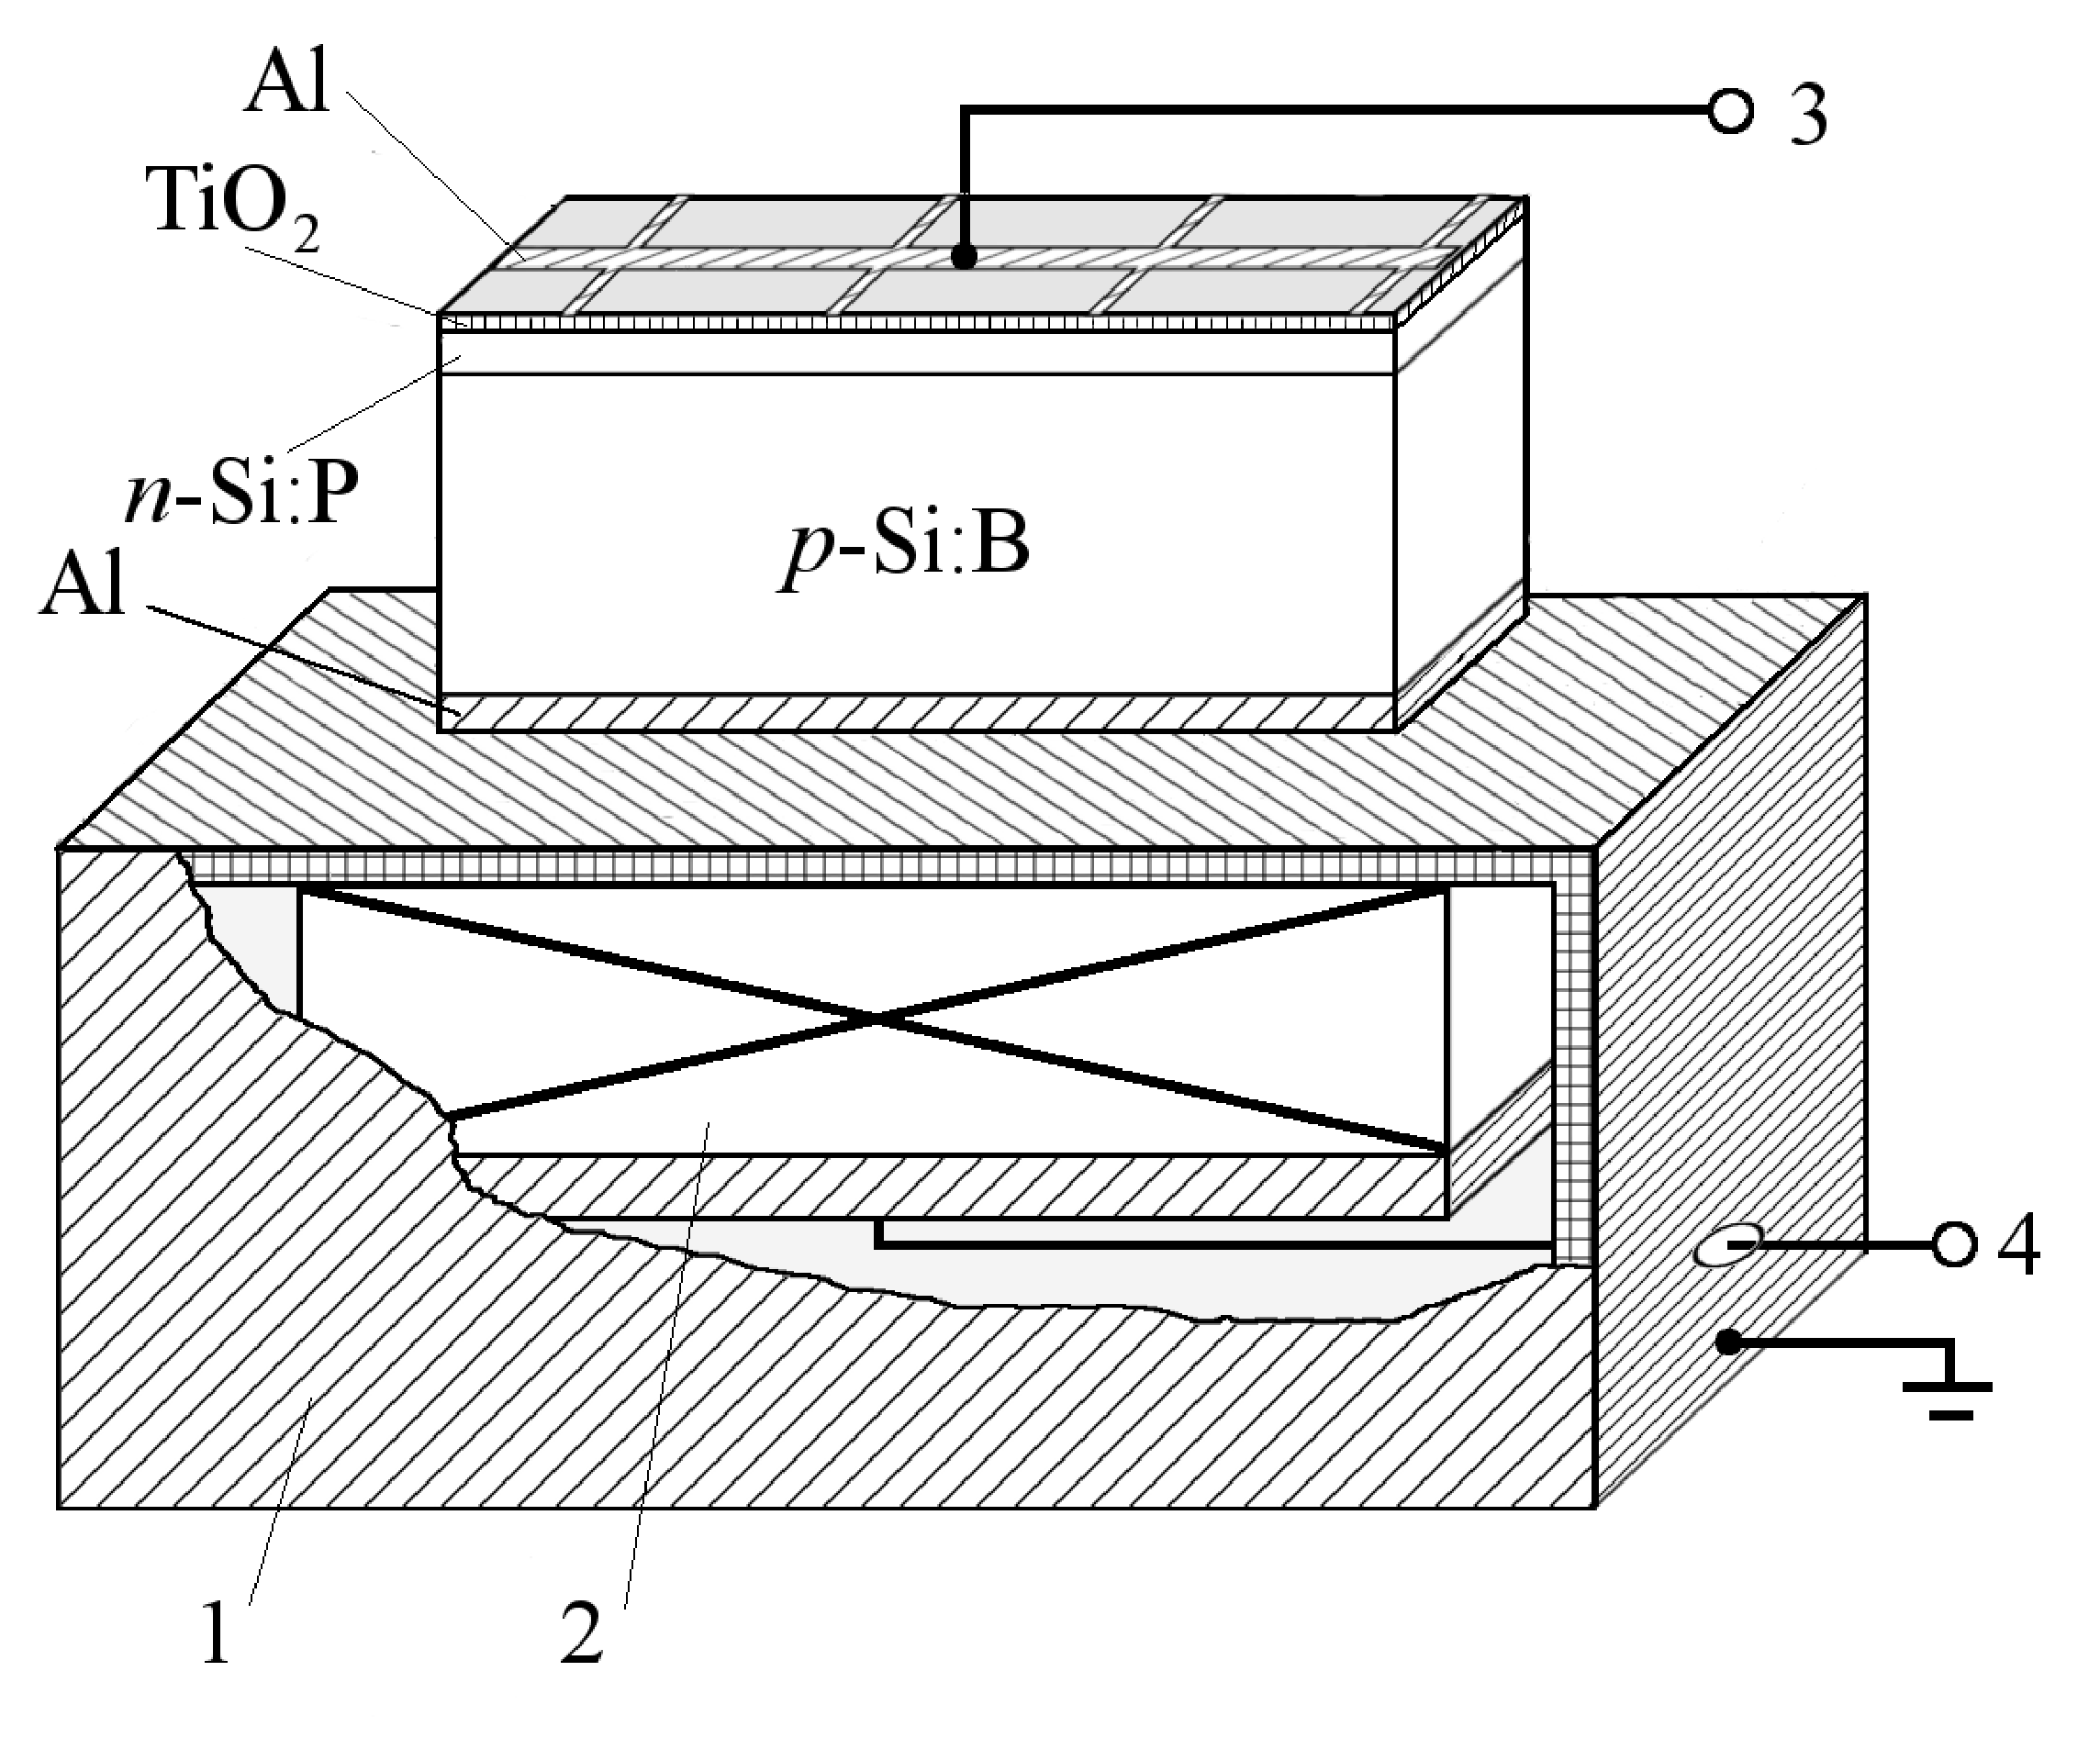
\includegraphics[width=0.6\textwidth]{USL_SC}%
\caption{\label{figUSL:SC}
Cхема УЗН кремнієвих сонячних елементів.
1 --  екран (алюмінієва фольга, товщина 0,012 мм);
2 --- п'єзоелектричний перетворювач (LiNbO$_3$);
3 --- контакти для вимірювання ВАХ;
4 --- контакти для збудження УЗ.
}
\end{figure}


Для оцінки інтенсивності АХ введеної у кремнієву структуру використовувалася формула плоского п’єзоперетворювача \cite{WusBook}:
 \begin{equation}
 \label{eqWus}
 W_\mathtt{US}=4K_\mathtt{LNO}^2C_\mathtt{LNO}f_r\frac{\rho_\mathtt{LNO}\,\upsilon_\mathtt{LNO}}{\rho_\mathtt{Si}\,\upsilon_\mathtt{Si}}\frac{V_\mathtt{RF}^2}{A_\mathtt{LNO}M_0},
 \end{equation}
де
$K_\mathtt{LNO}$ --- коефіцієнт електромеханічного зв'язку,
$C_\mathtt{LNO}$ та $A_\mathtt{LNO}$ --- статична ємність закріпленого перетворювача та його площа, відповідно;
для використаних в роботі перетворювачів ємність складала $(1\div3)\cdot10^{-10}$~Ф залежно від площі та товщини;
$f_r$ --- резонансна частота;
$\rho_\mathtt{LNO}$ та $\rho_\mathtt{Si}$ --- густина LiNbO$_3$ та кремнію, відповідно;
$\upsilon_\mathtt{LNO}$ та $\upsilon_\mathtt{Si}$ --- швидкості поширення звуку в ніобаті літію та Si, відповідно;
$V_\mathtt{RF}$ --- амплітуда високочастотної напруги, прикладеної до перетворювача,
а коефіцієнт $M_0$ розраховується за допомогою співвідношення
 \begin{equation}
 \label{eqM0}
 M_0=\frac{\left[\cos\left(\pi\frac{f_\mathtt{US}}{f_r}\right)\right]^2+\left[\frac{\rho_\mathtt{LNO}\,\upsilon_\mathtt{LNO}}{\rho_\mathtt{Si}\,\upsilon_\mathtt{Si}}\sin\left(\pi\frac{f_\mathtt{US}}{f_r}\right)\right]^2}
 {\left[\sin\left(\frac{\pi}{2}\frac{f_\mathtt{US}}{f_r}\right)\right]^4}.
 \end{equation}
При цьому при поширенні АХ має місце відносна деформація
 \begin{equation}
 \label{eqDefUS}
 \xi_{\mathtt{US}}=\sqrt{\frac{2W_\mathtt{US}}{\rho_\mathtt{Si}\,\upsilon_\mathtt{Si}^3}},
 \end{equation}
а амплітуда зміщень атомів
 \begin{equation}
 \label{eqAmpUS}
 u_{\mathtt{US}}=\sqrt{\frac{W_\mathtt{US}}{2\,\pi^2\,f_\mathtt{US}^2\,\rho_\mathtt{Si}\,\upsilon_\mathtt{Si}}}.
 \end{equation}

Параметри, які використовувалися при розрахунках, наведено в Таблиці~\ref{tabLNO}.


\begin{table}
\caption{\label{tabLNO}Деякі параметри ніобату літію та кремнію при кімнатній температурі \cite{WusBook,ShackBook}.
}
%\begin{tabular}{|l|l|c|}
%\begin{tabularx}{\textwidth}{|>{\raggedright\arraybackslash}X|>{\centering\arraybackslash}X|>{\centering\arraybackslash}X|}
\begin{tabularx}{\textwidth}{|l|>{\centering\arraybackslash}X|>{\centering\arraybackslash}X|}
\hline
$K_\mathtt{LNO}^2$&зріз $(Y\!+\!36^\circ)$&0,24\\
\cline{2-3}
&зріз $(Y\!+\!163^\circ)$&0,46\\
\hline
$\upsilon_\mathtt{LNO}$,&повздовжні хвилі&7340\\
\cline{2-3}
м/с&поперечні хвилі&4560\\
\hline
&повздовжні хвилі, $[100]$&8430\\
\cline{2-3}
&повздовжні хвилі, $[111]$&9850\\
\cline{2-3}
$\upsilon_\mathtt{Si}$,&повздовжні хвилі, $[110]$&9130\\
\cline{2-3}
м/с&поперечні хвилі, $[110]\,/\,[1\bar{1}0]$&4670\\
\cline{2-3}
&поперечні хвилі, $[110]\,/\,[001]$&5840\\
\cline{2-3}
&поперечні хвилі, $[111]\,/\,$довіл.&5090\\
\hline
\multicolumn{2}{|l|}{$\rho_\mathtt{LNO}$, кг/м$^3$}&4700\\
\hline
\multicolumn{2}{|l|}{$\rho_\mathtt{Si}$, кг/м$^3$}&2328\\
\hline
%\end{tabular}
\end{tabularx}
\end{table}

Дослідження проводились у достатньо вузькому температурному діапазоні $290\div340$~К.
При цьому вважалось, що параметри п'зоелектричного перетворювача змінюються мало, сталість величини $V_\mathtt{RF}$ забезпечує незмінність $W_\mathtt{US}$  для всього діапазону температур.
Вплив металевого екрануючого прошарку на інтенсивність звуку, введеного в зразок, вважався знехтувано малим, так як їх товщина значно менша ніж половина довжини АХ.



Параметри УЗ навантажень КСЕ, їх позначення та зразки, до яких вони застосовувалися, наведено в Таблиці~\ref{tabUSL}.

\begin{table}
\caption{\label{tabUSL}Параметри ультразвукових навантажень КСЕ.
}
%\center
\begin{tabular}{|c|c|c|c|c|c|c|c|}
\hline
$f_\mathtt{US}$,&Тип&$W_{\mathtt{US}}$,&$\xi_{\mathtt{US}}$,&$u_{\mathtt{US}}$,&$T$,&УЗН&Зразок\\
МГц&хвиль&Вт/см$^2$&$10^{-6}$&нм&K&&\\
\hline
8,0&повздовжні&0,18&1,3&0,30&302$\div$333&U--L&SC11, SC17\\ \hline
4,2&поперечні&0,19&2,9&0,63&300$\div$340&U--Ts1&SC17, g7SC12\\ \hline
4,2&поперечні&0,22&3,1&0,67&295$\div$335&U--Ts2&SC11\\ \hline
4,2&поперечні&0,24&3,2&0,70&300$\div$340&U--Ts3&nSC4\\ \hline
4,2&поперечні&0,37&4,0&0,87&308$\div$340&U--Tb1&g7SC12\\ \hline
4,2&поперечні&0,38&4,1&0,89&308$\div$340&U--Tb2&g6SC8\\ \hline
4,2&поперечні&0,40&4,2&0,91&310$\div$340&U--Tb3&SC11, SC17\\
&&&&&&&nSC4\\ \hline
8,0&повздовжні&до 1,5&до 5,1&до 0,86&290$\div$330&U--L8&SC13, nSC7\\ \hline
26,1&повздовжні&до 0,26&до 1,9&до 0,1&290$\div$333&U--L26&SC13, nSC7\\ \hline
%4,1&повздовжні&0,02& 0,7& 0,19&$\sim$300&U--L4t&SC3\\ \hline
%4,1&повздовжні&0,18& 1,6& 0,52&$\sim$300&U--L4t&SC3\\ \hline
%4,1&повздовжні&0,30& 2,1& 0,68&$\sim$300&U--L4t&SC3\\ \hline
%4,1&повздовжні&0,44& 2,5& 0,82&$\sim$300&U--L4t&SC3\\ \hline
4,1&повздовжні&до 0,65&до 3,0&до 1,0&$\sim$300&U--L4t&SC3, SC11A\\ \hline
%4,1&повздовжні&0,09& 3,0& 1,0&$\sim$300&U--L4t&SC10\\ \hline
%4,1&повздовжні&0,20& 3,0& 1,0&$\sim$300&U--L4t&SC10\\ \hline
%4,1&повздовжні&0,25& 3,0& 1,0&$\sim$300&U--L4t&SC10\\ \hline
%4,1&повздовжні&0,43& 3,0& 1,0&$\sim$300&U--L4t&SC10\\ \hline
8,0&повздовжні&до 0,09&до 1,1&до 0,19&$\sim$300&U--L8t&SC11A\\ \hline
13,6&повздовжні&до 0,15&до 1,5&до 0,15&$\sim$300&U--L13t&SC3\\ \hline
26,1&повздовжні&до 0,10&до 1,2&до 0,06&$\sim$300&U--L26t& SC11A\\ \hline
\end{tabular}
\end{table}




\section{Оборотна акусто--керована деградація неопромінених кристалічних кремнієвих сонячних елементів\label{USID}}

На сьогодні КСЕ продовжують відігравати домінуючу роль у галузі фотовольтаїки, займаючи приблизно три чверті відповідного ринку.
Основними причинами є достатньо високий рівень коефіцієнта корисної дії, доступність та нетоксичність сировини,
низька ціна та високий рівень розвитку технологічних процесів, необхідних для їх виготовлення \cite{Si:Hu}.
Першочерговою задачею виробників КСЕ (як і інших напівпровідникових пристроїв) є можливість керування їх властивостями,
що, насамперед, пов'язане з розумінням причинно--наслідкових зв'язків процесів, які відбуваються під час фотогенерації та руху носіїв заряду.
Наприклад, виявлено, що зменшення ефективності роботи КСЕ може відбуватися внаслідок
\begin{enumerate}[label=\asbuk*),leftmargin=0em,itemindent=1.5em]
  \item інтенсивного освітлення --- процес, який у випадку СЕ на основі кристалічного кремнію носить назву LID (light--induced degradation) \cite{LID:SchmidtJMR,LIDRev,LIDRev2,LID:JAP2017II}, тоді як для мікрокристалічного Si широко використовується абревіатура CID (carrier-induced degradation) \cite{CID:APL,CID:PPS};
  \item прикладання високої (декілька сотень вольт і більше) напруги --- PID  (potential--induced degradation) \cite{PID:SEMSC,PID:PP,PID:2017};
  \item радіаційного опромінення ---  RID (radiation--induced degradation) \cite{Bhat,Karazhanov}.
\end{enumerate}
Причинами деградації є зміни у дефектній підсистемі кристалів.
Це може бути перебудова комплексів бор--кисень або комплексів, які містять мідь (для випадку LID),
декорування дефектів пакування позитивно зарядженими іонами, переважно, натрію, що спричинює зменшення шунтуючого опору (PID)
або утворення радіаційних рекомбінаційних центрів (RID).
Відпал деградованих КСЕ при підвищених температурах нерідко дозволяє повністю (або частково) відновити ефективність.

В той же час, УЗ також здатний ефективно взаємодіяти з дефектами в кремнії.
Наприклад, було експериментально показано що УЗ викликає трансформацію домішкових та радіаційних дефектів \cite{Korotchenkov1995,Ostapenko1995,UST:Medvid,YOlikh:SupMicr},
модифікацію спектру \cite{Zaver:2008} та густини \cite{Mirsagatov} поверхневих станів,
зміну дифузійної довжини електронів \cite{Ostapenko1999,Ostrovskii2001}
та впливає на проходження струму у бар'єрних структурах \cite{Davletova2009,Davletova2008,YOlikh2005}.
Детальніше ці ефекти описані в розділі~\ref{Oglyad}.
Тобто, цілком очікуваним є те, що внаслідок поширення АХ в КСЕ може виникати ефект акусто--індукованої деградації (USID, ultrasound--induced degradation).
При використанні УЗ не надто високої інтенсивності, параметри матеріалу після припинення поширення АХ повертаються до вихідних значень \cite{Ostapenko1999,Ostrovskii2001,Korotchenkov1995} навіть без застосування відпалу.
Тому очікується, що USID має бути оборотною при кімнатних температурах на відміну від деградацій інших типів.
Представлені у даному параграфі результати отримані в результаті експериментального дослідження АІ змін фото--електричних параметрів КСЕ.

\subsection{Особливості визначення параметрів КСЕ\label{sbSSCMethod}}
Для визначення параметрів КСЕ проводилось вимірювання у режимі постійного струму прямих ділянок ВАХ зразків у темряві та при освітленні.
Вимірювання проводились в температурному інтервалі  290--340~K як за умов УЗН, так і без нього.
Приклад декількох залежностей наведено на Рис.~\ref{figSSCIV}.

\begin{figure}
\center
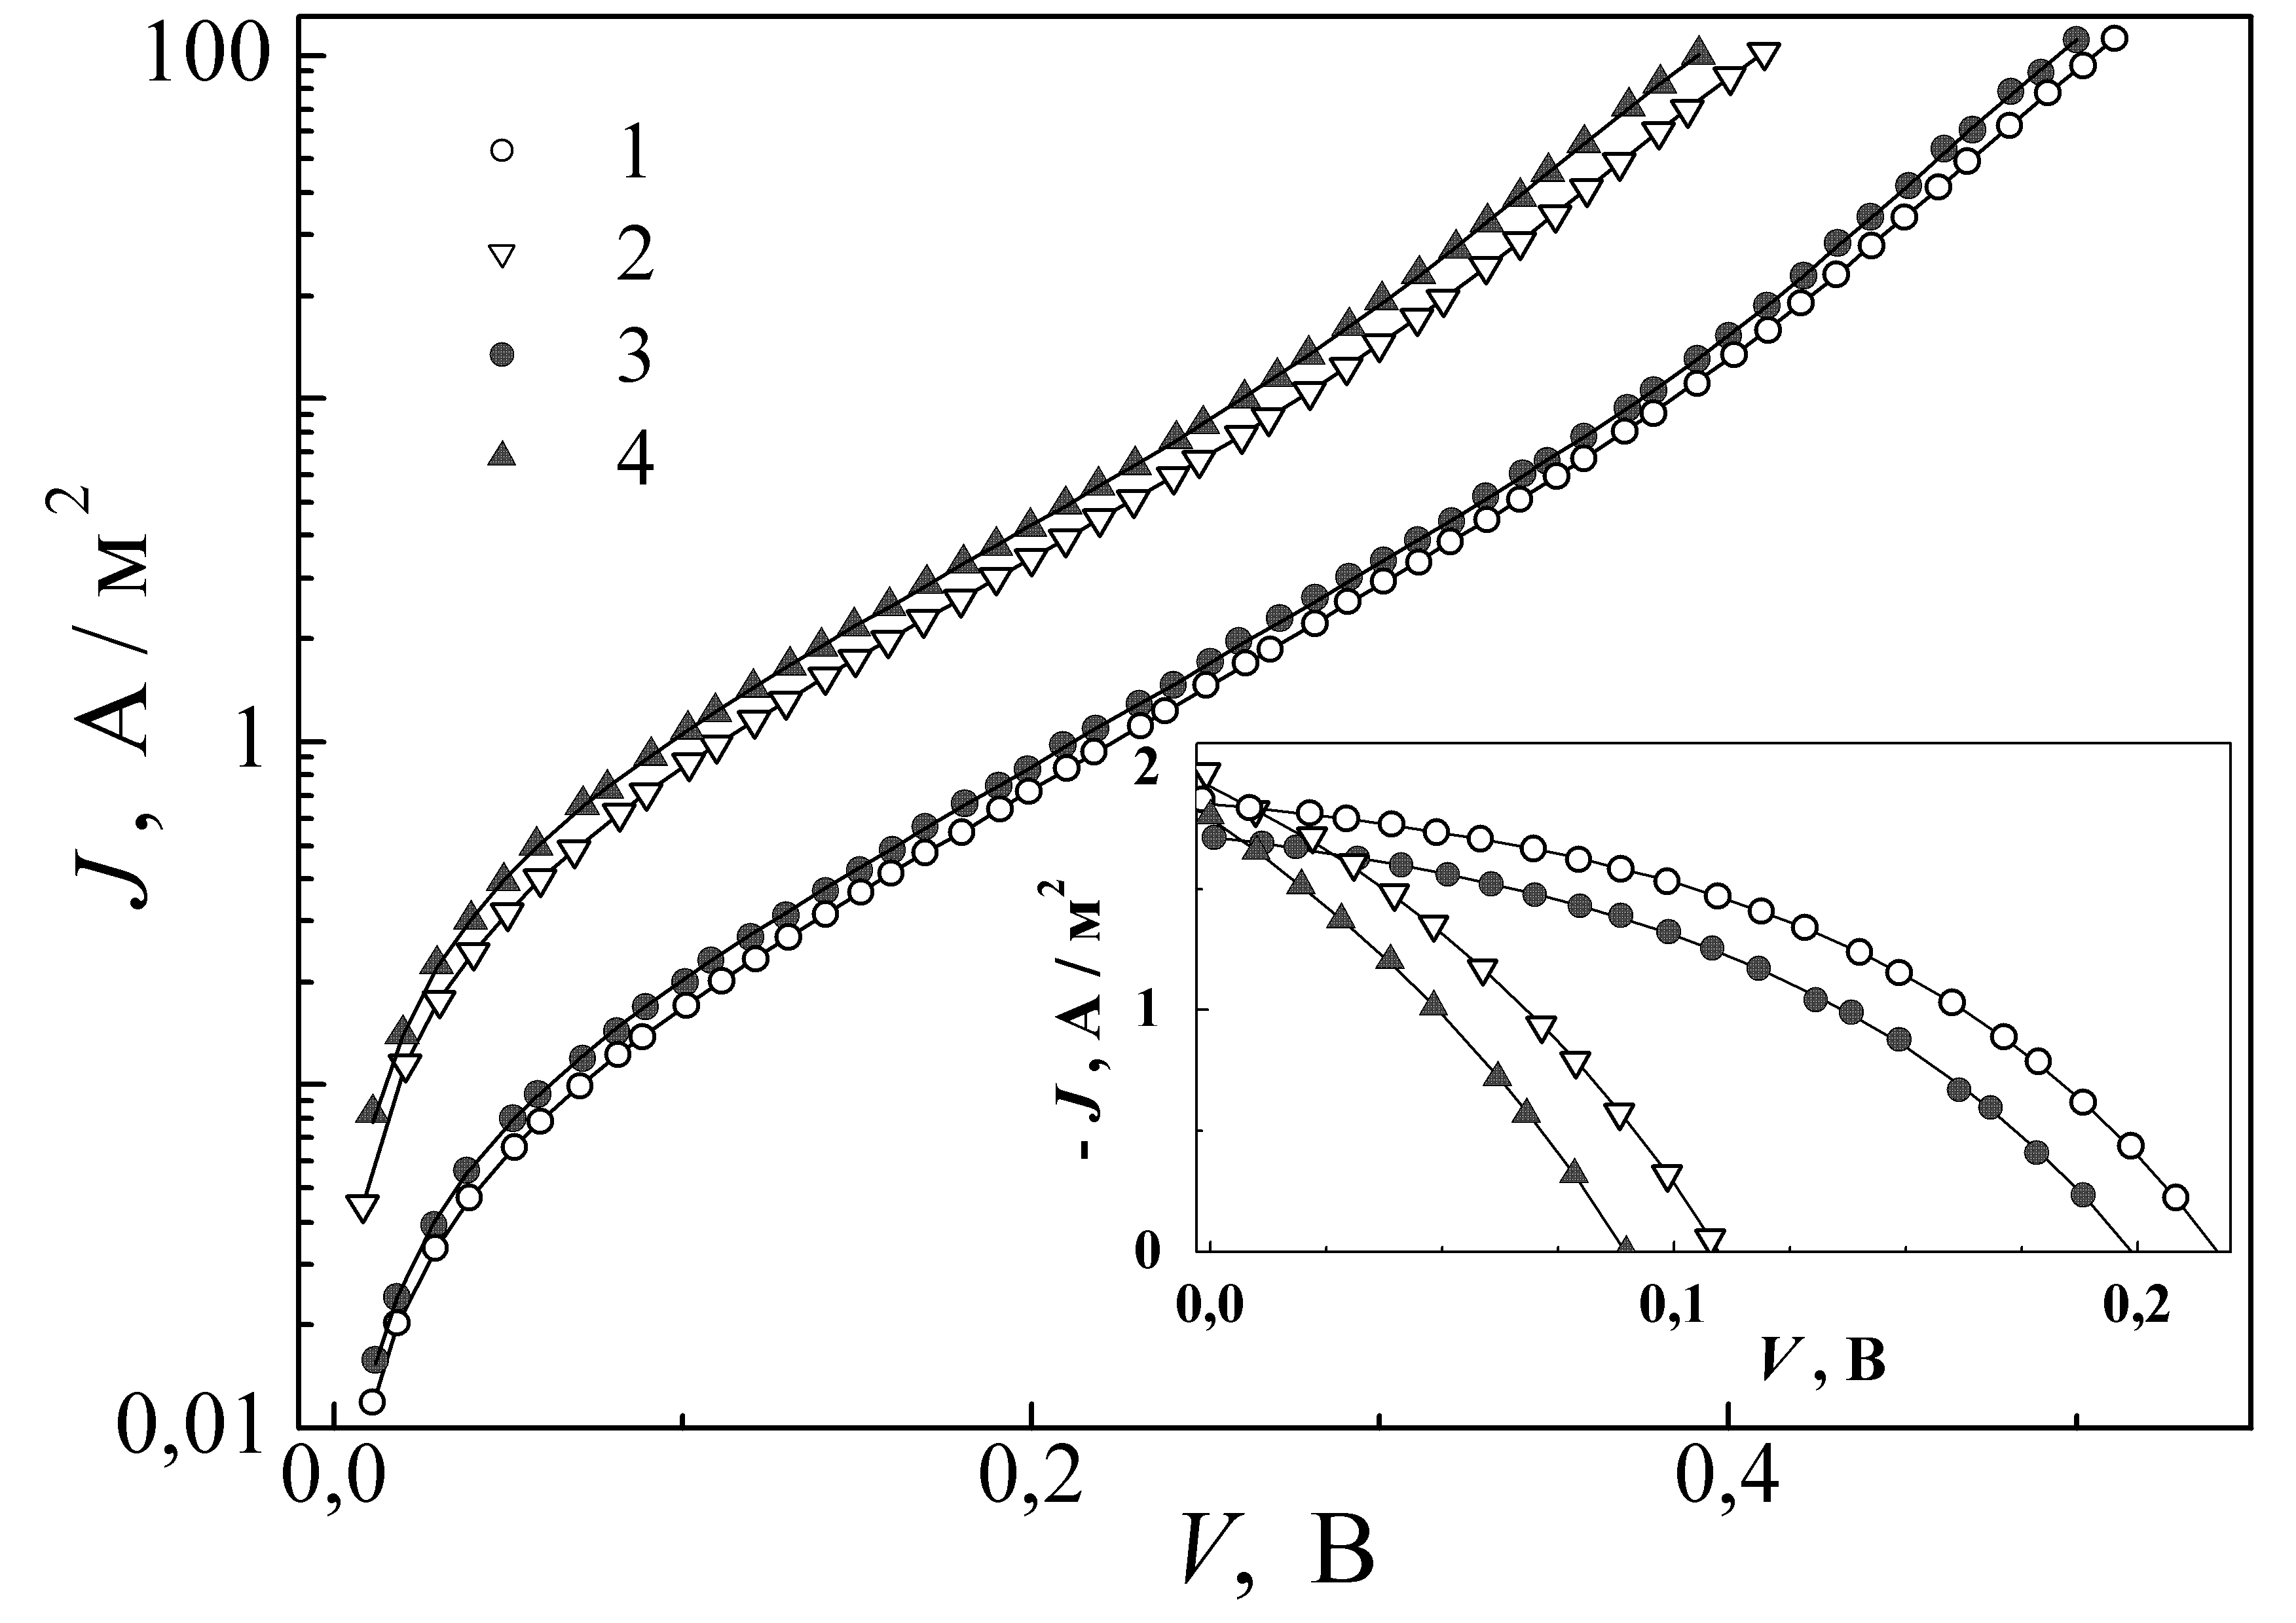
\includegraphics[width=0.9\textwidth]{figSSCIV}%
\caption{\label{figSSCIV}
Темнові ВАХ, виміряні при температурах 301~K (криві 1 та 2, кола) та 341~K (криві 2 та 4, трикутники)
за умов УЗН (U--Tb3, криві 2, 4, заповнені точки) та для ненавантаженого зразка (криві 1 та 3, порожні точки)
На вставці наведено частину ВАХ при освітлені в діапазоні прямих зміщень від 0 до $V_{oc}$.
Точки відображають результати вимірів, лінії отримані шляхом апроксимації за формулами (\ref{eqSSCIV}) та (\ref{eqW}).
%(\labelcref{eqSSCIV,eqW}) \ref{eqW}.
}%
\end{figure}

Густина струму короткого замикання $J_{sc}$, напруга холостого ходу $V_{oc}$ та фактор форми $F\!F$ визначалися з ВАХ, отриманих при освітленні,
традиційним способом за перетином експериментальної кривої з координатними осями  та по розташуванню максимуму потужності.

В рамках моделі подвійного діоду залежність густини струму $J$ від прикладеної напруги $V$ для  n$^+$--p сонячного елементу має описуватися
наступним виразом \cite{2Diod:Ishaque,2Diod:Buhler}:

\begin{eqnarray}
\label{eqSSCIV}
\nonumber J(V,\,T)&=&\left(I_{SCR}+I_{base}+I_{sh}\right)/A=\\
\nonumber &=&-J_{ph}+\frac{qn_id}{2\tau_{g}}\left\{\exp \left[\frac{q(V-JR_s)}{n_\mathrm{id}kT}\right]-1\right\}+\\
&&+\frac{qn_i^2}{p_p}\sqrt{\frac{\mu_nkT}{\tau_n}}\left\{\exp \left[\frac{q(V-JR_s)}{kT}\right]-1\right\}+\frac{V-JR_s}{R_{sh}}\,,
\end{eqnarray}
де
$I_{SCR}$ описує загальну рекомбінацію в області просторового заряду (ОПЗ)
$I_{base}$ пов'язане з процесами рекомбінації у квазі--нейтральній області (КНО),
$I_{sh}$ --- шунтуючий струм,
$A$ --- площа діоду,
$T$ --- абсолютна температура,
$J_{ph}$ --- густина фотогенерованого струму,
$q$ --- елементарний заряд,
$n_i$ --- концентрація власних носіїв заряду,
$\tau_{g}$  --- ефективний час життя носіїв заряду в ОПЗ,
$d$ --- товщина ОПЗ:
\begin{equation}
\label{eqW}
    d(V,\,T)=\sqrt{\frac{2 \varepsilon \varepsilon_0(p_p+n_n)}{q p_p n_n}\left[\frac{E_g}{q}-\frac{kT}{q}\ln\left(\frac{N_vN_c}{p_pn_n}\right)-\frac{2kT}{q}-V\right]} \,,
\end{equation}
$\varepsilon_0$ --- діелектрична стала,
$\varepsilon$ --- діелектрична проникність матеріалу (для Si $\varepsilon=11,7$),
$p_p$ та $n_n$ --- концентрація основних носіїв заряду в $p$-- та $n$--області, відповідно;
$E_g$ --- ширина забороненої зони напівпровідника,
$N_c$ та $N_v$ --- ефективна густина станів поблизу дна зони провідності та вершини валентної зони, відповідно;
$n_\mathrm{id}$ --- фактор неідеальності
$R_s$ та $R_{sh}$ --- послідовний та шунтуючий опори, відповідно;
$\mu_n$ та $\tau_n$ --- рухливість та час життя електронів (неосновних носіїв) в базі діоду.
Тобто,
рівняння ВАХ, яке моделює поведінку сонячного елементу за допомогою еквівалентної електричної схеми,
містить ряд параметрів, що безпосередньо стосуються фізичних процесів, які відбуваються у пристрої.
%Зокрема вважається, що
%$J_{0base}=(qn_i^2/n_n)\sqrt{\mu_nkT/\tau_n}$ пов'язане з процесами рекомбінації у квазі--нейтральній області (КНО), тоді як
%$J_{0SCR}=(qdn_i/2\tau_{g})$ описує загальну рекомбінацію в ОПЗ.

Формули (\ref{eqSSCIV})--(\ref{eqW}) були використані для апроксимації експериментальних даних, причому
невідомими величинами вважалися $\tau_g$, $\tau_n$, $n_{\mathrm{id}}$, $R_{sh}$, $R_s$ та  $J_{ph}$ (остання лише для ВАХ при освітленні).
При цьому вважалося, що
$n_i(T)=1,64\cdot10^{15}\,T^{1,706}\exp(-E_g/2kT)$~см$^{-3}$ \cite{ni:Green}, $N_c(T)=2,86\cdot10^{19}(T/300)^{1,58}$~см$^{-3}$, $N_v(T)=3,10\cdot10^{19}(T/300)^{1,85}$~см$^{-3}$
\cite{Nc:Green},
а температурні залежності забороненої зони та рухливості електронів описуються формулами Varshni та Caughey--Thomas, відповідно:
\begin{equation}
\label{eqEg}
 E_g(T) = E_g(0) - \frac{\beta_1 T^2}{(T + \beta_2)}\,,
\end{equation}
де
$E_g(0)=1,169$~еВ,
$\beta_1=7,021\cdot10^{-4}$~еВ/К$^2$,
$\beta_2=1108$~K \cite{Schroder2006,Markvart} та
\begin{equation}
\label{eqMu}
\mu_n(T) = \mu_{min}+\frac{\mu_0}{1+(p_p/N_{ref})^{\zeta}}\,.
\end{equation}
де
$\mu_{min}=92\cdot(T/300)^{-0,57}$~см$^2$/(В$\cdot$с),
$\mu_0=1268\cdot(T/300)^{-2,33}$~см$^2$/(В$\cdot$с),
$N_{ref}=1,3\cdot10^{17}\cdot(T/300)^{2,4}$~см$^{-3}$,
$\zeta=0,91\cdot(T/300)^{-0,146}$ \cite[с.~505, Table~A8.2]{Schroder2006}.
Апроксимація проводилась з використанням методу диференційної еволюції\cite{DE:Sun,DEWang,DEModif}, який більш детально описано в параграфі~\ref{subEA}.
Приклади результуючих апроксимуючих кривих наведено  на Рис.~\ref{figSSCIV}.
Видно, що вони досить добре апроксимують експериментальні дані.

Відомо \cite{2Diod:Buhler}, що $J_{sc}\approx J_{ph}R_{sh}/(R_{sh}+R_{s})$.
Для всіх досліджених зразків величина $R_s$ приблизно дорівнювала 2~Ом$\cdot$см$^2$, тоді як значення $R_{sh}$ суттєво залежала від температури та конкретного зразка, проте для
розглянутого температурного інтервалу не було меншим  4~кОм$\cdot$см$^2$.
Отже, очікується, що в нашому випадку має бути $J_{sc}\approx J_{ph}$.
І дійсно, подібне співвідношення спостерігається між величиною $J_{ph}$, отриманою шляхом багатопараметричної апроксимації
повної залежності густини струму від напруги, та значенням $J_{sc}$, яке відображає ординату перетину ВАХ з віссю струмів.

Для освітлення КСЕ використовувалося монохроматичне (довжина хвилі $\lambda=900$~нм) світло з низькою інтенсивністю.
Відомо, що освітлення з інтенсивністю $W_{ph}$ більше 5~Вт/см$^2$ викликає дисоціацію пар залізо--бор \cite{LID:CuII},
а при $W_{ph}>0.01$~suns (1~sun$=1000$~Вт/м$^2$) в кремнії р--типу утворення дефектів можуть утворюватись дефекти \cite{BO:Halam2016}.
Ці процеси впливають на час життя носіїв заряду, а так як метою роботи було дослідження АІ ефектів,
то з метою запобігання будь--яких світло--індукованих деградаційних процесів було використане
освітлення з інтенсивністю $W_{ph}=(8\pm4)$~Вт/м$^2$.
Монохроматичність світла дозволила спростити аналіз причин АІ змін струму короткого замикання.
А саме, для використаної довжини хвилі фотогенерований струм пов'язаний, переважно, з утворенням електронно--діркових пар в $p$--області.
У випадку, якщо база СКЕ перевищує у декілька разів довжину дифузії неосновних носіїв $L_n=\sqrt{\mu_nkT\tau_n/q}$, то
для $J_{sc}$ справедливий вираз \cite{Markvart,Razeghi,Faren}:
\begin{equation}
\label{eqIph}
J_{sc} = \frac{W_{ph}(1-R_{ph})q\beta\lambda}{hc}\frac{\alpha L_n}{1+ \alpha L_n}\,,
\end{equation}
де
$\alpha$ --- коефіцієнт поглинання світла,
$R_{ph}$ --- коефіцієнт відбивання,
$\beta$ --- коефіцієнт квантового виходу.

Формулу~(\ref{eqIph}) було використано для апроксимації експериментальної залежності $J_{sc}(T)$,
при чому $L_n$ розглядалась як невідомий параметр.
Під час розрахунків вважалося, що $R_{ph}$ та $\beta$ не змінюються (згідно з \cite{Gaman}, для кремнію
при використаній довжині хвилі $\beta=1$),
а температурна залежність $\alpha$ описується виразом \cite{Markvart,Si:Absorb}
\begin{eqnarray}
\label{eqAlpha}
\nonumber \alpha(\lambda,\,T)&=&\sum_{\substack{i=1,2\\j=1,2}}\!C_iA_j\left\{\frac{[hc/\lambda-E_{gj}(T)+E_{p\,i}]^2}{\exp(E_{p\,i}/kT)-1}\:+
\frac{[hc/\lambda-E_{gj}(T)-E_{p\,i}]^2}{1-\exp(-E_{p\,i}/kT)}\right\}+\\
&&+A_d\left[hc/\lambda-E_{gd}(T)\right]^{1/2}\,,
\end{eqnarray}
де
$h$ --- стала Планка,
$c$ --- швидкість світла,
$E_{p\,1}=1,827\cdot10^{-2}$~еВ,
$E_{p\,2}=5,773\cdot10^{-2}$~еВ --- частоти Дебая поперечних
оптичних та акустичних фононів, відповідно;
константи $C_1=5,5$,
$C_2=4,0$,
$A_1=3,231\cdot10^2$~см$^{-1}$еВ$^{-2}$,
$A_2=7,237\cdot10^3$ см$^{-1}$еВ$^{-2}$,
$A_d=1,052\cdot10^6$ см$^{-1}$еВ$^{-2}$;
температурна залежність $E_{g1}$, $E_{g2}$ та $E_{gd}$ описується виразом \ref{eqEg}),
причому $E_{g1}(0)=1,169$~еВ, $E_{g2}(0)=2,5$~еВ та $E_{gd}(0)=3,2$~еВ.
Крім того, припускалося що $L_n\sim T^{0.5}$.
Основою для цього були результати, отримані при апроксимації окремих ВАХ (детальніше див. параграф~\ref{sbQNR}).

Таким чином, визначення $L_n$ та $\tau_n$ проводилось як в результаті аналізу окремої ВАХ, так і з апроксимації
температурної залежності $J_{sc}$.
Надалі, щоб відрізнити величини, отримані другим шляхом, використовується верхній індекс <<$ph$>>: $L_n^{ph}$, $\tau_n^{ph}$, $\varepsilon_{\tau n}^{ph}$ тощо.

Ще раз підкреслимо, що всі АІ ефекти, описані у цьому розділі є оборотними.
Тобто, величини $J_{sc}$, $V_{oc}$, $F\!F$ та інших параметрів повертаються до своїх вихідних значень
після припинення УЗН  та витримки зразків при кімнатній температурі протягом доби.
Оборотність АІ ефектів ілюструє Рис.~\ref{figReverse}.
Часовий інтервал між початком УЗН та вимірами, результати яких представлені з позначкою <<під час УЗН>>
перевищує 60~хв, проміжок часу між закінченням УЗН та вимірами <<після УЗН>> --- близько 24~год.
На рисунку представлені дані лише для двох зразків, але ці результати є типовими і для інших.
Оборотність ефектів, зокрема, свідчить про те, що УЗ не спричинює ні дифузію дефектів,
ні зміну їх концентрації.

\begin{figure}
\center
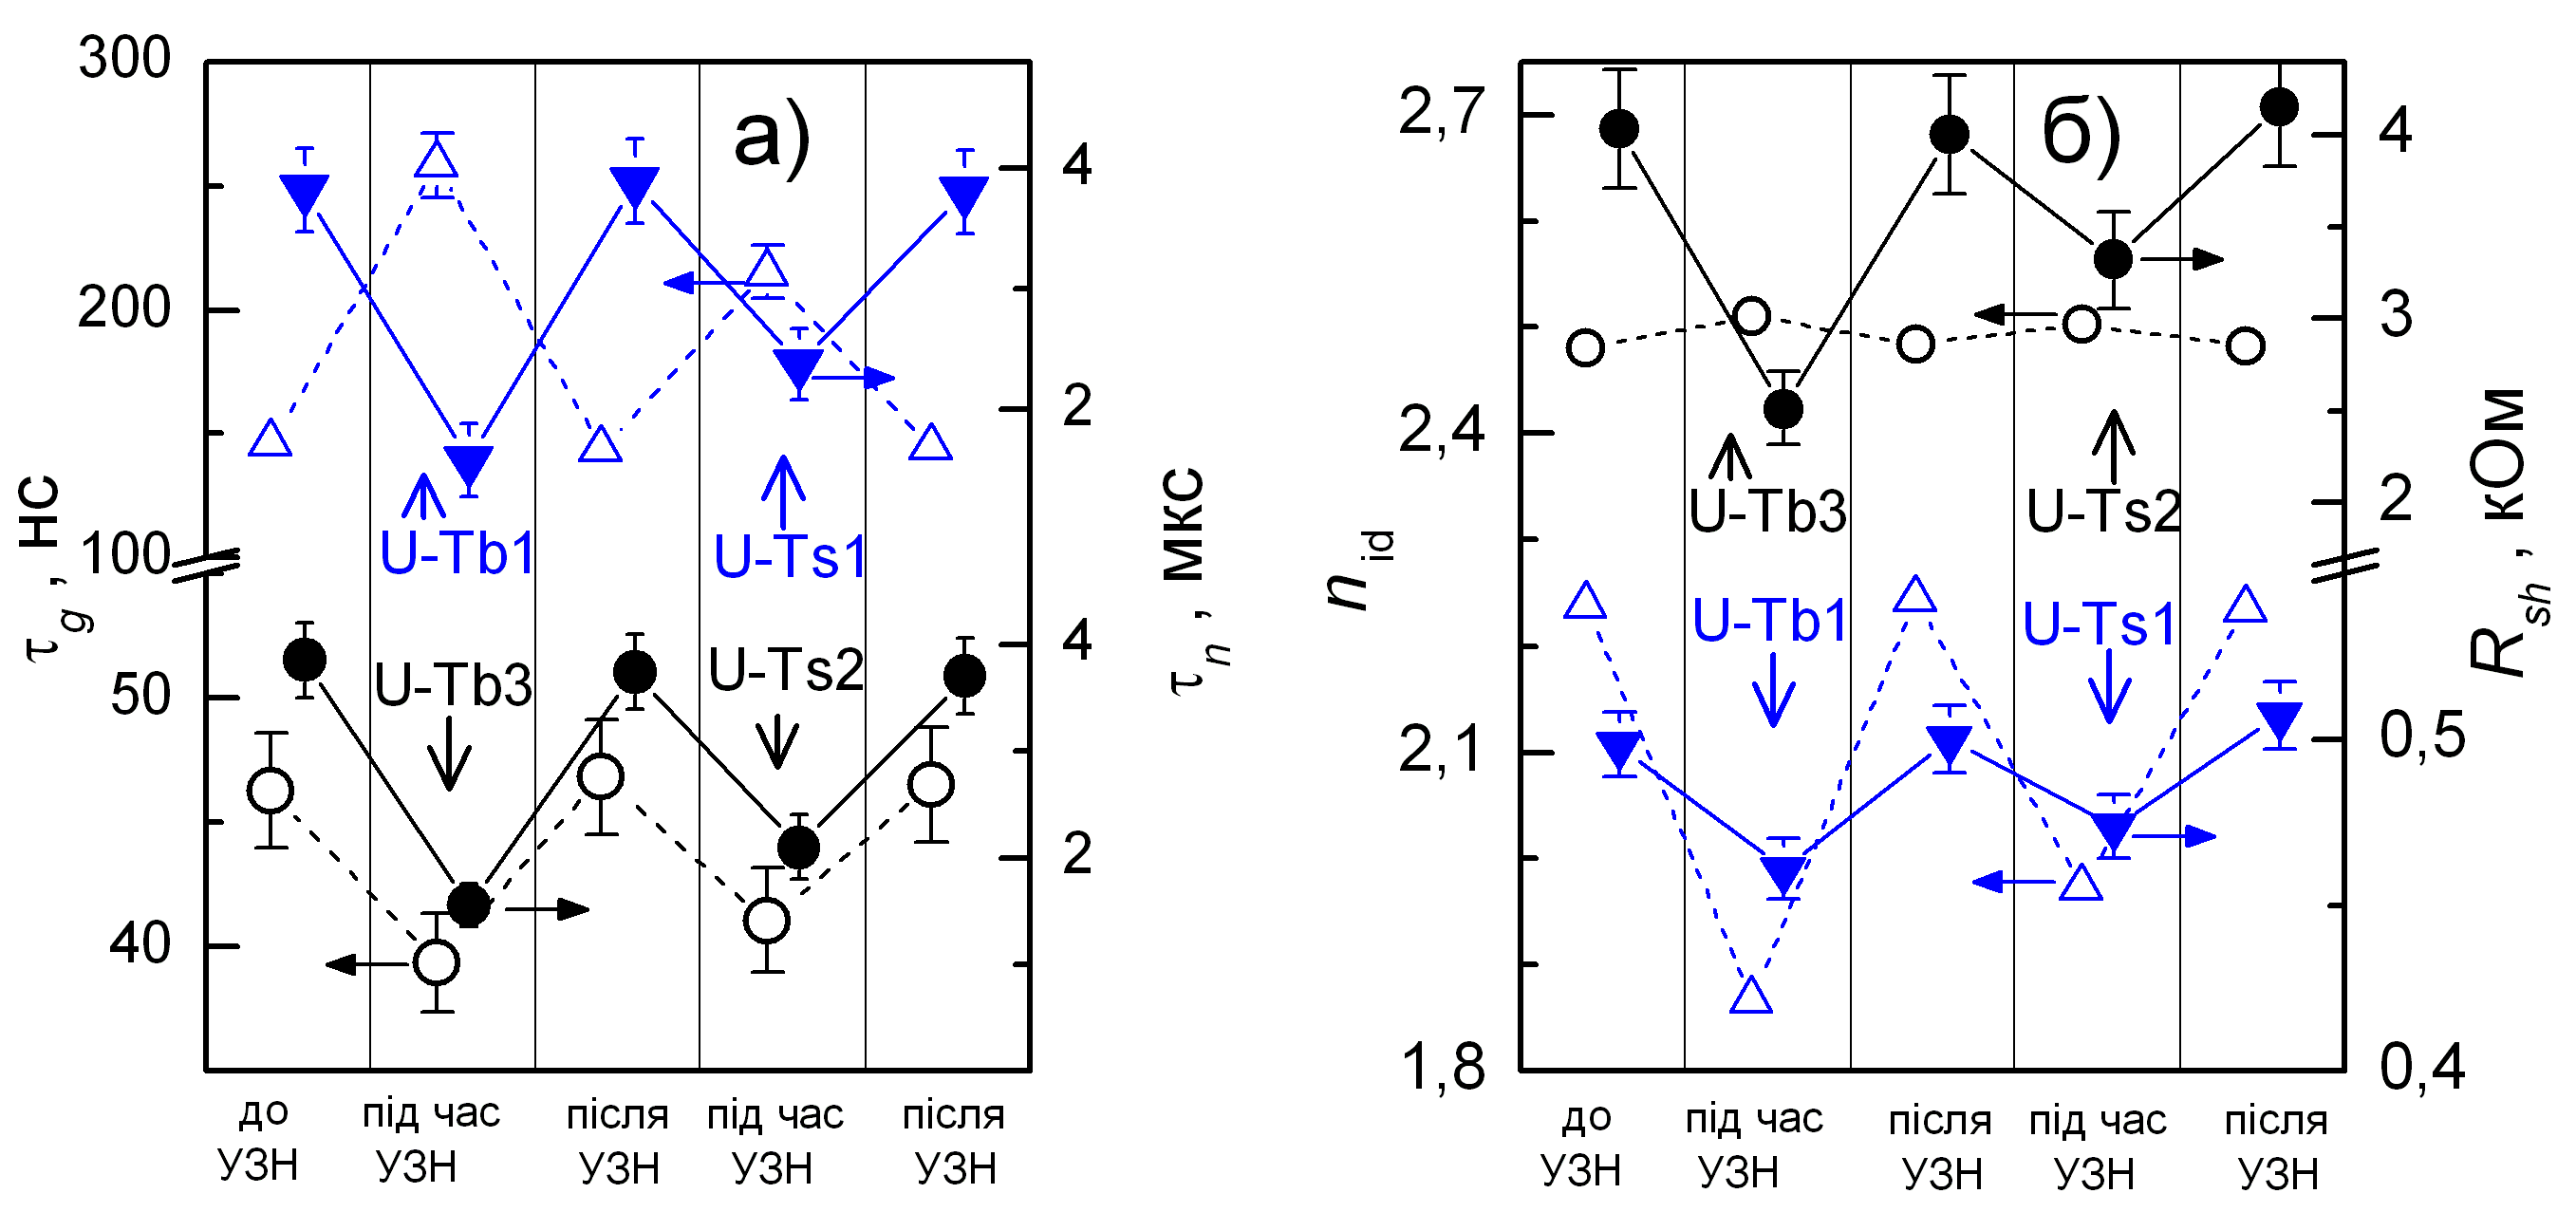
\includegraphics[width=1\textwidth]{figReverse}%
\caption{\label{figReverse}
Значення часу життя в ОПЗ (a, ліва вісь, незаповнені точки)
та КНО (a, права вісь, заповнені точки),
фактору неідеальності (б, ліва вісь, незаповнені точки) та
шунтуючого опору (б, права вісь, заповнені точки),
отримані до, під час та після УЗН при температурі 330~K.
Представлені дані для зразків SC11 (кола) та g7SC12 (трикутники).
}%
\end{figure}


Зауважимо, що величини параметрів ($\tau_g$, $\tau_n$, $n_{\mathrm{id}}$, $R_{sh}$ та $R_s$) отримані з ВАХ, які виміряні у темряві та при освітленні за однакової температури
та в ідентичних умовах УЗН, практично збігаються.


Відомо, що дефекти розподіляються по площі напівпровідникових пластин нерівномірно (див., наприклад, \cite{Oxide:Chen,Oxide_Schon}),
а отже, нерівномірним є і розподіл фізичних параметрів.
В нашому випадку також спостерігався розкид величин визначених параметрів зразків, вирізаних з різних частин вихідної пластини (див. Рис.~\ref{figSSC},б).
Проте характер АІ змін цих параметрів для всіх зразків був подібний.
Тому з усього набору досліджених структур (5 зразків) надалі в цьому параграфі представлено типові результати переважно лише для двох (SC11 та SC17),
вихідні параметри яких відрізнялися найбільше.



\subsection{Вплив ультразвукового навантаження на фотоелектричне перетворення в КСЕ}

Отримані температурні залежності густини струму короткого замикання, напруги холостого ходу та фактору форми наведено на Рис.~\ref{figDUSIsc}.
Значення параметрів при температурі 320~K представлені в Таблиці~\ref{tabSSCParam}.
Необхідно зауважити, що не тільки $J_{sc}$ та $V_{oc}$, але й коефіцієнт корисної дії, $F\!F$ та час життя неосновних носіїв
заряду зменшуються за умов низько-інтенсивного освітлення \cite{LI:Ruhle,LI:Reich,LI:lifetime}.
А отже, дані на Рис.~\ref{figDUSIsc} та в Таблиці~\ref{tabSSCParam} не є еквівалентними тим, що
можуть бути отримані за стандартних умов (STC, standard test condition, інтенсивність освітлення 1000~Вт/м$^2$,
температура $25^{\circ}$C, спектр AM1.5G).
Проте вони ілюструють АІ ефекти.


%\begin{figure}[b]
\begin{figure}
\center
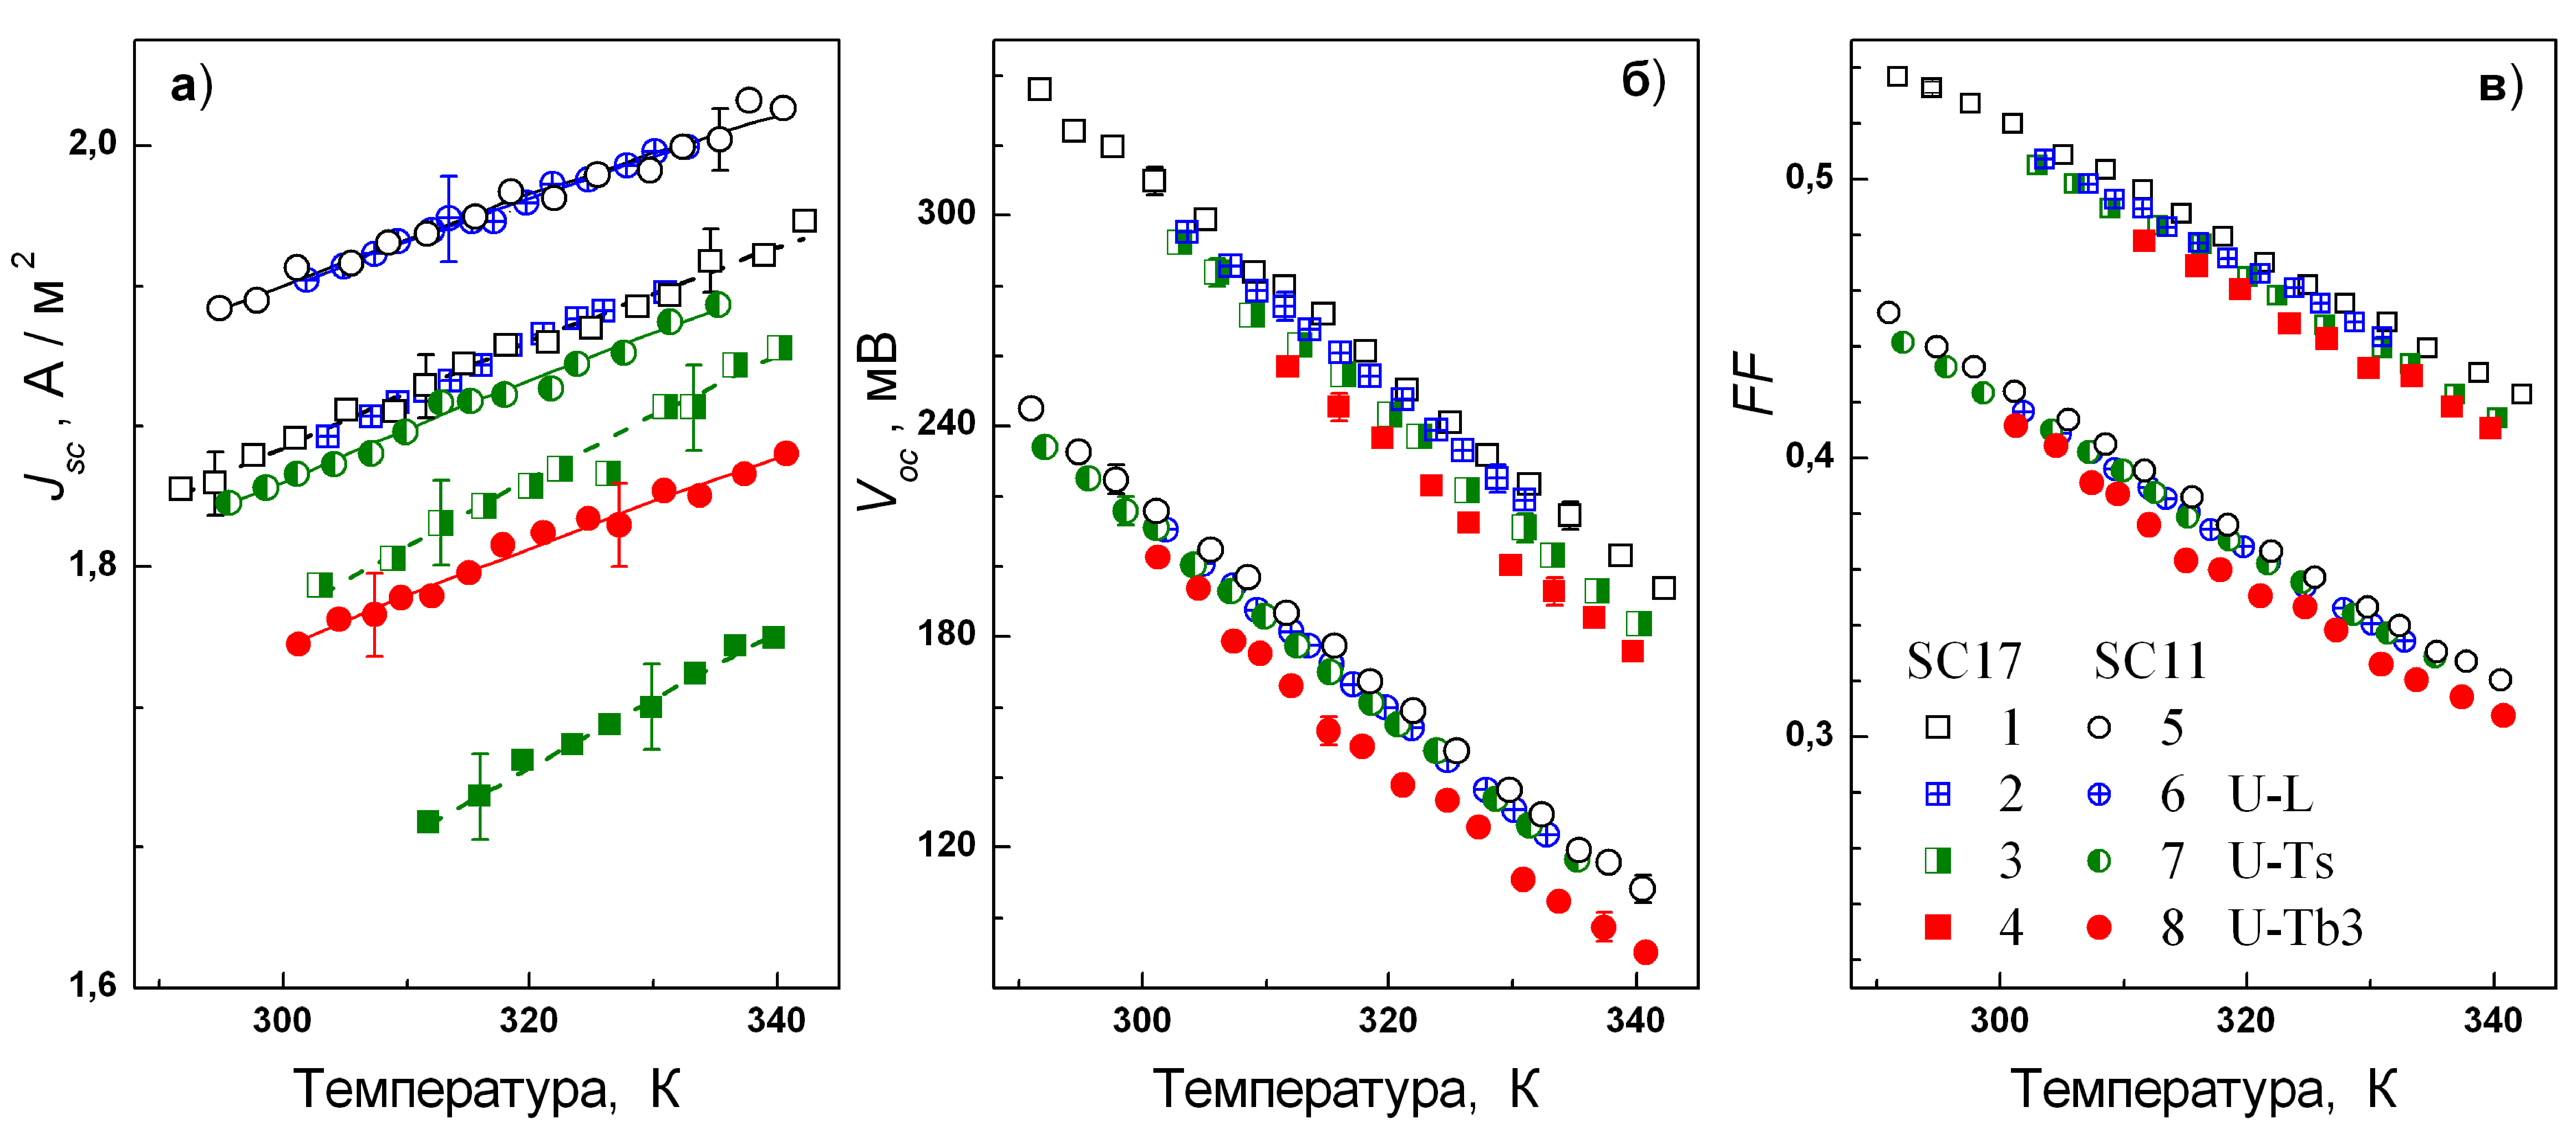
\includegraphics[width=1\textwidth]{figDUSIsc}%
\caption{\label{figDUSIsc}
Температурна залежність густини струму короткого замикання (а),
напруги холостого ходу (б) та
фактору форми (в)
для структур SC17 (квадрати) and SC11 (кола).
\FigCaptionSSC
%Криві 1 та 5 (незаповнені символи) отримані без УЗН,
%решта --- під час УЗН: U--L (криві 2 та 6),
%U--Ts1 (3),  U--Ts2 (7) та U--Tb3 (4 та 8).
Точки відповідають експериментально отриманим результатам,
лінії --- результати апроксимації згідно з формулою~(\ref{eqIph}).
}%
\end{figure}


\begin{table}
\caption{\label{tabSSCParam}Визначені параметри КСЕ ($T=320$~K).
}
\small
\begin{tabular}{|l|c|c|c|c|c|c|c|c|}
\hline
&\multicolumn{4}{c|}{SC17}&\multicolumn{4}{|c|}{SC11}\\
Параметр&\multicolumn{4}{c|}{УЗН}&\multicolumn{4}{|c|}{УЗН}\\ \cline{2-9}
&---&U--L&U--Ts1&U--Tb3&---&U--L&U--Ts2&U--Tb3\\
%\hline
\hhline{|=========|}
$J_{sc}$, 0.01A/м$^2$&191$\pm$2&191$\pm$2&184$\pm$2&171$\pm$2&198$\pm$2&198$\pm$2&189$\pm$2&181$\pm$2\\ \hline
$V_{oc}$, мВ&256$\pm$4&250$\pm$4&243$\pm$4&233$\pm$4&164$\pm$4&159$\pm$4&157$\pm$4&141$\pm$4\\ \hline
$F\!F$, $10^{-3}$&475$\pm$2&468$\pm$2&463$\pm$2&458$\pm$2&372$\pm$2&366$\pm$2&366$\pm$2&353$\pm$2\\ \hline
$L_n^{ph}$, мкм&99$\pm$5&92$\pm$5&67$\pm$4&55$\pm$3&125$\pm$6&124$\pm$6&103$\pm$5&98$\pm$5\\ \hline
$L_n$, мкм&93$\pm$5&82$\pm$4&47$\pm$3&34$\pm$2&106$\pm$5&99$\pm$5&80$\pm$4&69$\pm$4\\ \hline
$\tau_n^{ph}$, $10^{-7}$ с$^*$&31$\pm$3&26$\pm$3&14$\pm$2&9$\pm$1&49$\pm$5&48$\pm$5&33$\pm$4&30$\pm$3\\ \hline
$\tau_n$, $10^{-7}$ с&26$\pm$3&21$\pm$3&7$\pm$2&3.5$\pm$0.7&35$\pm$3&31$\pm$3&20$\pm$3&15$\pm$2\\ \hline
$\tau_g$, $10^{-9}$ с&70$\pm$4&66$\pm$3&57$\pm$3&48$\pm$2&35$\pm$2&31$\pm$2&30$\pm$2&29$\pm$2\\ \hline
$E_{\tau g}$, меВ&242$\pm$7&237$\pm$5&234$\pm$5&234$\pm$5&245$\pm$6&234$\pm$5&241$\pm$5&243$\pm$5\\ \hline
$n_\mathrm{id}$, $\pm$0.01&2.59&2.60&2.61&2.63&2.51&2.52&2.53&2.54\\ \hline
$T_\mathrm{id}$, K&226$\pm$8&215$\pm$10&243$\pm$15&233$\pm$15&327$\pm$10&319$\pm$15&308$\pm$20&358$\pm$25\\ \hline
$K_\mathtt{US}$, м$^{-2}$с$^{-1}$&\multicolumn{4}{c|}{(3.3$\pm$0.5)$\times10^{24}$}&\multicolumn{4}{|c|}{(5.0$\pm$0.2)$\times10^{23}$}\\ \hline
$R_{sh}$, кОм$\cdot$см$^2$&$>10^{12}$&$>10^{12}$&$>10^{12}$&$>10^{12}$&12$\pm$1&13$\pm$1&10$\pm$1&8$\pm$1\\ \hline
%\multicolumn{9}{l}{$^*$ determined by using the whole temperature range}
\end{tabular}
\end{table}

Так, Рис.~\ref{figDUSIsc} показує, що має місце акусто--керована деградація як струму короткого замикання, так і напруги холостого ходу та
фактора форми.
Відносні АІ зміни  параметрів наведено в Таблиці~\ref{tabAIEfect}.
Зауважимо, величина АІ змін слабко залежить від температури у розглянутому температурному діапазоні практично для всіх параметрів, які розглядались в роботі.


\begin{table}
\caption{\label{tabAIEfect}Акусто--індуковані зміни параметрів КСЕ.
}
\center
%\begin{tabular}{|c|c|c|c|c|c|c|}
\begin{tabularx}{\textwidth}{| >{\centering\arraybackslash}X|
                              >{\centering\arraybackslash}X|
                              >{\centering\arraybackslash}X|
                              >{\centering\arraybackslash}X|
                              >{\centering\arraybackslash}X|
                              >{\centering\arraybackslash}X|
                              >{\centering\arraybackslash}X|
  }
\hline
&\multicolumn{3}{c|}{SC17}&\multicolumn{3}{|c|}{SC11}\\
Параметр&\multicolumn{3}{c|}{УЗН}&\multicolumn{3}{|c|}{УЗН}\\ \cline{2-7}
&U--L&U--Ts1&U--Tb3&U--L&U--Ts2&U--Tb3\\
%\hline
\hhline{|=======|}
%&\multicolumn{3}{|c|}{SC17}&\multicolumn{3}{c|}{SC11}\\  \hline
%Параметр&U--L&U--Ts1&U--Tb3&U--L&U--Ts2&U--Tb3\\ \hline
$\varepsilon_{Jsc}$, \%&0$\pm$1&4$\pm$1&10$\pm$1&0$\pm$1&5$\pm$1&9$\pm$1\\ \hline
$\varepsilon_{Voc}$, \%&2$\pm$2&5$\pm$2&9$\pm$2&3$\pm$2&4$\pm$2&14$\pm$2\\ \hline
$\varepsilon_{F\!F}$, \%&2$\pm$1&3$\pm$1&4$\pm$1&2$\pm$1&2$\pm$1&5$\pm$1\\ \hline
$\varepsilon_{Ln}^{ph}$, \%&7$\pm$7&32$\pm$7&44$\pm$7&1$\pm$7&18$\pm$7&22$\pm$7\\ \hline
$\varepsilon_{Ln}$, \%&12$\pm$6&49$\pm$6&63$\pm$6&6$\pm$6&25$\pm$6&35$\pm$6\\ \hline
$\varepsilon_{\tau n}^{ph}$, \%&16$\pm$15&55$\pm$15&70$\pm$15&2$\pm$15&33$\pm$15&39$\pm$15\\ \hline
$\varepsilon_{\tau n}$, \%&19$\pm$12&73$\pm$12&87$\pm$12&11$\pm$12&43$\pm$12&57$\pm$12\\ \hline
$\varepsilon_{\tau g}$, \%&6$\pm$5&19$\pm$5&31$\pm$5&9$\pm$5&14$\pm$5&17$\pm$5\\ \hline
-$\Delta n_\mathrm{id}$, $10^{-2}$&1$\pm$1&2$\pm$1&4$\pm$1&1$\pm$1&2$\pm$1&3$\pm$1\\ \hline
$\varepsilon_{R sh}$, \%&&&&-8$\pm$10&17$\pm$10&33$\pm$10\\ \hline
%\end{tabular}
\end{tabularx}
\end{table}

Значення інтенсивності АХ під час УЗН U--L, U--Ts1 та U--Ts2 близькі (див. Таблицю~\ref{tabUSL}).
Проте наведені дані свідчать, що $J_{sc}$ та $V_{oc}$ більше змінюються під час U--Ts1 та U--Ts2, тобто при використанні поперечних хвиль.
В той же час, U--L та U--Ts відрізняються значеннями $f_\mathtt{US}$ та $u_\mathtt{US}$ ($\xi_\mathtt{US}$).
Проте раніше \cite{Olikh:FTP2011,Olikh:Ultras2016} було показано, що збільшенні частоти УЗН ефективність впливу ультразвуку
на кремнієві структури зростає.
Отже, ефективність УЗ дії на КСЕ визначається насамперед зміщенням атомів (деформацією ґратки),
а не інтенсивністю АХ (загальною енергією коливань, енергією яку отримує кристал під час УЗН).
З цієї точки зору поперечні АХ є більш ефективним інструментом впливу, ніж повздовжні,
так як за однакових енергетичних затрат дозволяють досягти більшого ефекту.

Рівняння (\ref{eqIph}) показує, $J_{sc}$ суттєво залежить від довжини дифузії неосновних носіїв.
Визначені шляхом апроксимації експериментальних залежностей значення $L_n^{ph}$ та розраховані на їх основі величини $\tau_n^{ph}$,
а також їх зміни в умовах УЗН наведено в Таблицях~\ref{tabSSCParam} та \ref{tabAIEfect}.
Лінії Рис.~\ref{figDUSIsc},a відображають результати апроксимації.
Отримані результати показують, що УЗ впливає на час життя неосновних носіїв і саме цим можна пояснити виявлені зміни струму короткого замикання в ультразвуковому полі.

На жаль, аналітичних виразів для $V_{oc}$ та $F\!F$ у випадку моделі подвійного діоду у літературі не запропоновано.
В той же час аналіз виразів на кшталт

\begin{eqnarray}
\label{eqSSCVoc}
 J_{sc}&=&\frac{qn_id}{2\tau_{g}}\left(e^{\frac{qV_{oc}}{n_\mathrm{id}kT}}-1\right)
+\frac{qn_i^2}{p_p}\sqrt{\frac{\mu_nkT}{\tau_n}}\left(e^{\frac{qV_{oc}}{kT}}-1\right)+\frac{V_{oc}}{R_{sh}}\,,\\
J_{sc}\left(2+\frac{R_s}{R_{sh}}\right)&=&\frac{qn_id}{2\tau_{g}}\left(e^{-\frac{qJ_{sc}R_s)}{n_\mathrm{id}kT}}-1\right)
+\frac{qn_i^2}{p_p}\sqrt{\frac{\mu_nkT}{\tau_n}}\left(e^{-\frac{qJ_{sc}R_s}{kT}}-1\right)
\end{eqnarray}
з одного боку дещо утруднений, проте з іншого показує напруга холостого ходу та фактор форми
залежать від $\tau_n$, $n_\mathrm{id}$, $\tau_g$, та $R_{sh}$.
У наступному параграфі розглянуто вплив УЗ на ці параметри.
Причини змін $V_{oc}$ та  $F\!F$ обговорені в параграфі~\ref{sbVocSim}.


\subsection{Особливості акустичного керування рекомбінацією в КСЕ\label{sbQNR}}

Традиційно, під час аналізу процесів, які відбуваються у структурах з $p-n$--переходом окремо розглядаються рекомбінацію в ОПЗ та в КНО.
Зокрема, вплив рекомбінації в ОПЗ є суттєвим для КСЕ (особливо з тиловою металізацією зокрема), які працюють в області низьких
освітленостей та при вимірах малосигнальних значень фото--ерс \cite{Sach:UPJ2016} --- тобто за умов, які відповідають нашим експериментам.


Параметрами ВАХ, які пов'язані з процесами в області просторового заряду є $n_{\mathrm{id}}$ та $J_{0SCR}=(qdn_i/2\tau_{g})$.
Під час аналізу отриманих результатів вважалося, що УЗ з невисокою інтенсивністю, використаний в роботі, не
викликає зміни параметрів напівпровідника, які визначаються основною ґраткою (тобто  $E_g$, $N_c$, $N_v$ тощо).
Тому замість розгляду величини $J_{0SCR}$ як цілого, основна увага була приділена $\tau_{g}$.
Отримані температурні залежності часу життя носіїв в ОПЗ та фактору неідеальності наведені на Рис.\ref{figDUS},a та Рис.~\ref{figDUS},б, відповідно.
Виявлено, що експериментальна температурна залежність $\tau_{g}$ цілком задовільно описується виразом
\begin{equation}
\label{eq_TAUgT}
    \tau_{g}(T)=\tau_{g0}\exp\left(-\frac{E_{\tau g}}{kT}\right)\:.
\end{equation}

\begin{figure}
\center
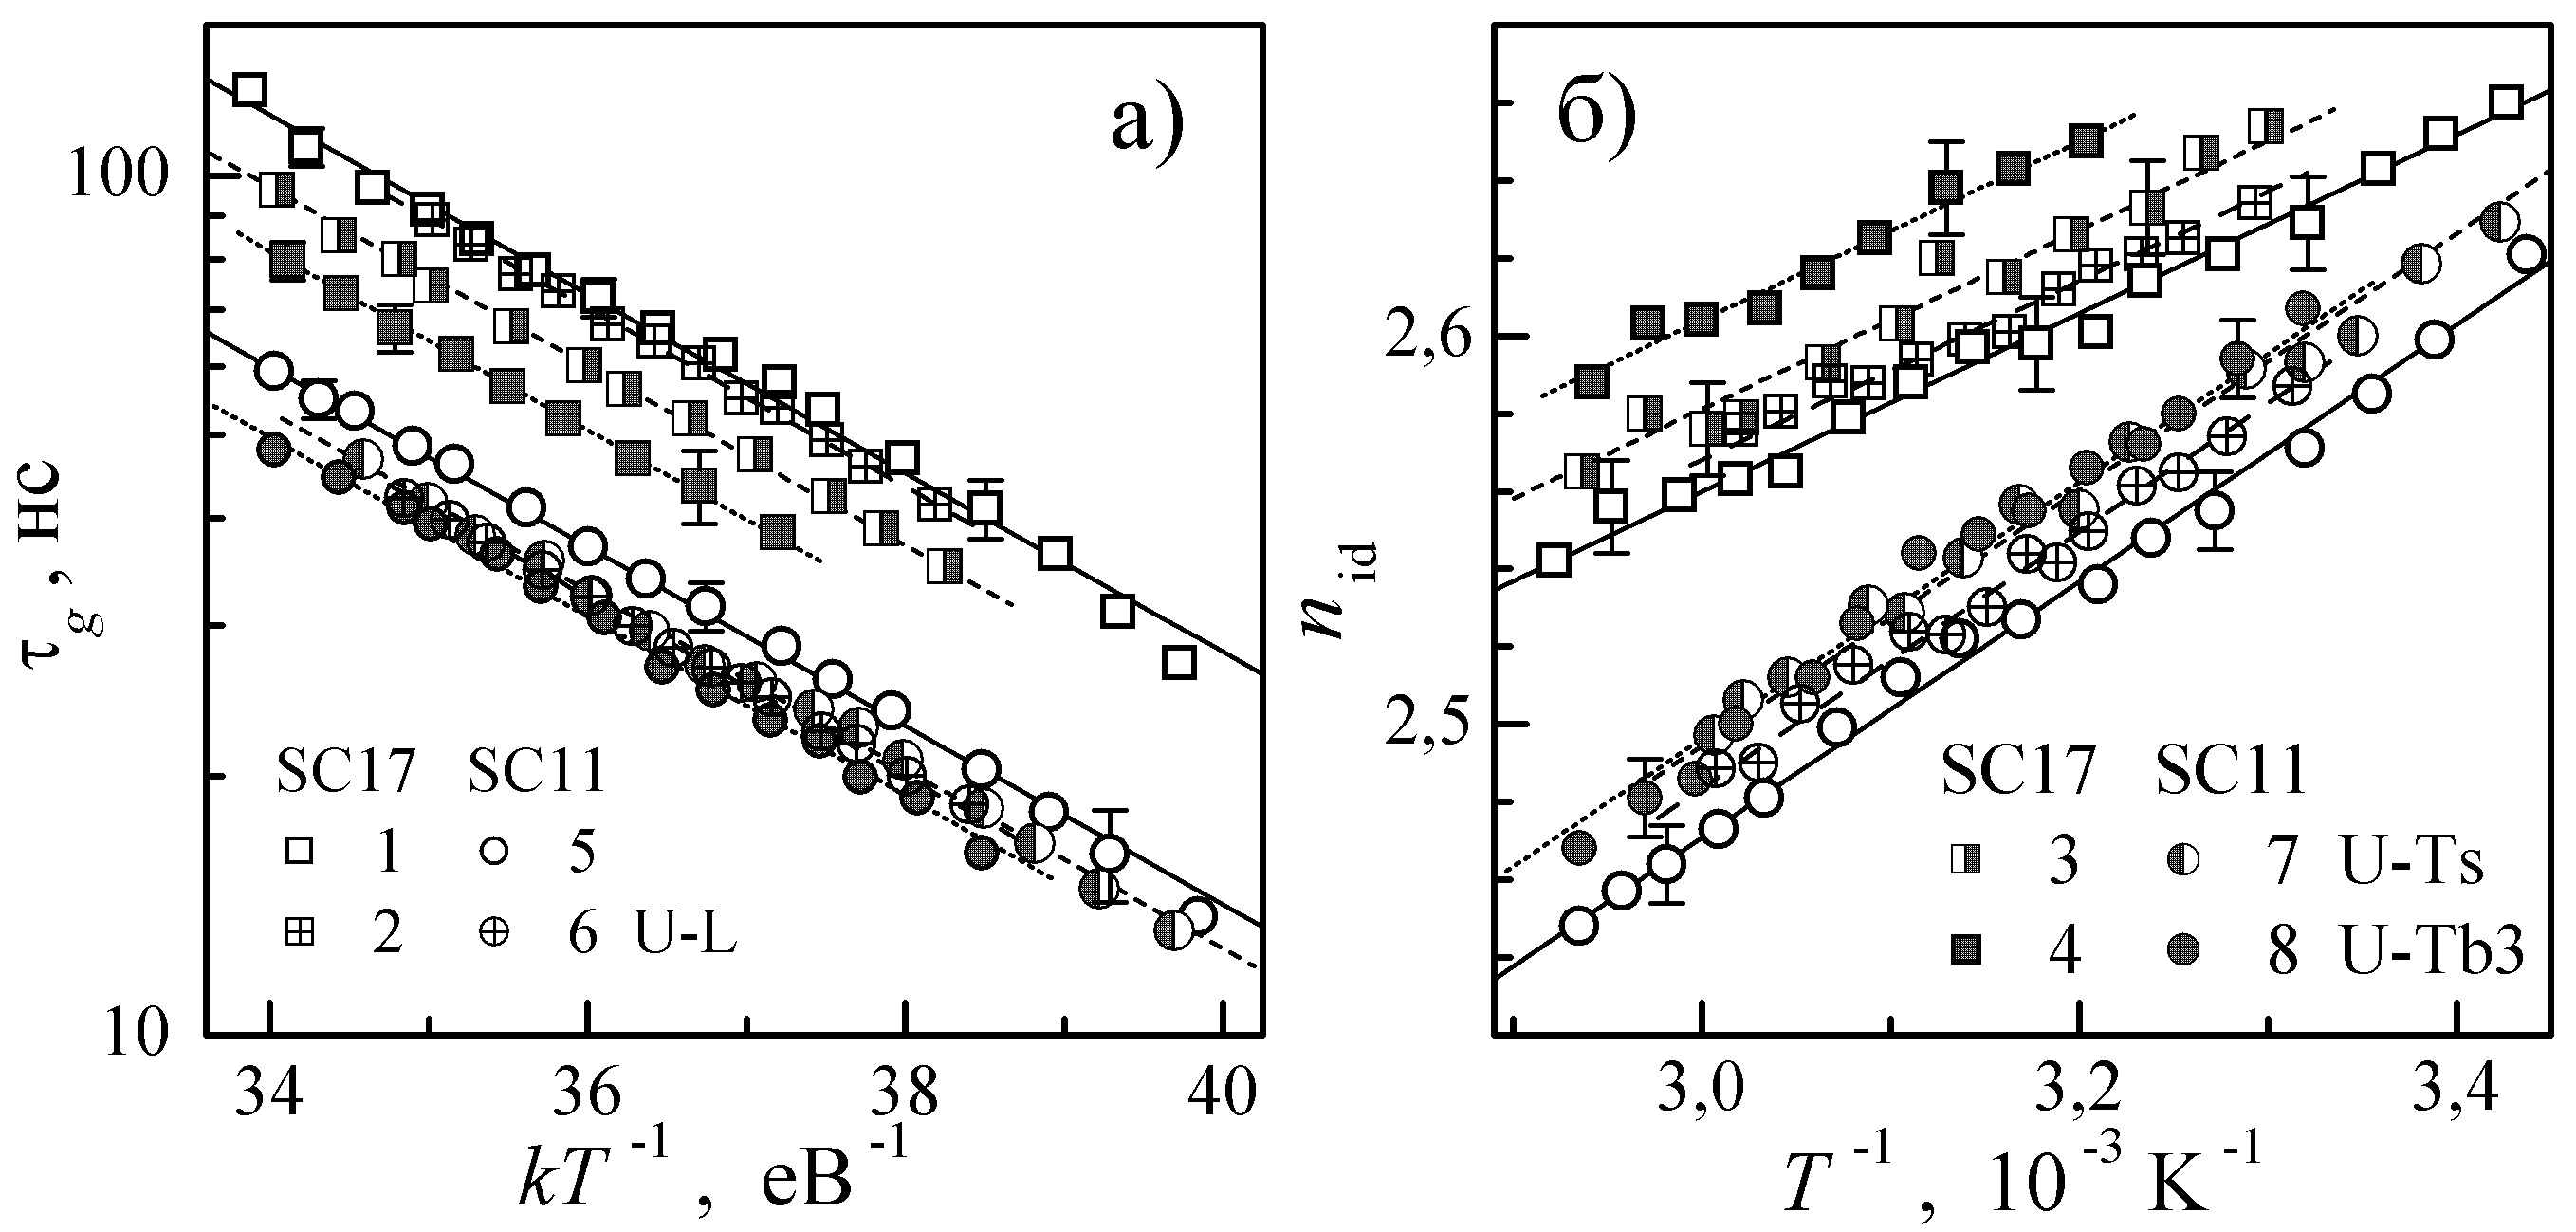
\includegraphics[width=1\textwidth]{figDUS}%
\caption{\label{figDUS}
Температурні залежності часу життя носіїв в ОПЗ (а) та фактору неідеальності (б)
для зразків SC17 (криві 1--4, квадрати) та SC11 (5--8, кола).
\FigCaptionSSC
Точки --- експеримент,
лінії -- результат апроксимації з використанням виразу~(\ref{eq_TAUgT}) і $E_{\tau g}=0.24$~eV (a) та
формули~(\ref{eq_nT}) і $T_\mathrm{id}=330$ або 230~K (б).
}%
\end{figure}

Як показано на Рис.~\ref{figDUS},б, фактор неідеальності зменшується зі зростанням температури, а залежність
$n_{\mathrm{id}}$ від $1/T$  близька до лінійної.
Таким чином, залежність $n_{\mathrm{id}}(T)$ може бути описана наступним чином
\begin{equation}
\label{eq_nT}
    n_{\mathrm{id}}(T)=n_{\mathrm{id},\infty}+T_{\mathrm{id}}/T\:.
\end{equation}
Величини $T_{\mathrm{id}}$ та $E_{\tau g}$, обчислені для зразків в умовах УЗН та без нього, наведено в Таблиці~\ref{tabSSCParam}.


Як видно з наведених на Рис.~\ref{figDUS} та в Таблиці~\ref{tabSSCParam} даних
\begin{enumerate}[label=\asbuk*),leftmargin=0em,itemindent=1.5em]
%\begin{enumerate}[label=\asbuk*),labelindent=0em,itemindent=1.5em]
\item УЗН призводить збільшення $n\mathrm{id}$ та зменшення $\tau_{g}$;
   величини АІ змін показано в Таблиці~\ref{tabAIEfect};
\item $\tau_{g}$ та $n\mathrm{id}$ змінюються більш ефективно при використанні поперечних АХ;
\item $\varepsilon_{\tau g}$ та $\Delta n_\mathrm{id}$ збільшуються при використанні УЗ з більшими значеннями $W_{\mathtt{US}}$;
\item УЗН не впливає на $E_{\tau g}$ та $T_\mathrm{id}$;
 $E_{\tau g}=0.24\pm0.01$~еВ для всіх досліджених зразків,
 тоді як характерна температура фактору неідеальності залежить від місця розташування зразка на пластині: $T_\mathrm{id}=330\pm30$~K для SC11 та $T_\mathrm{id}=230\pm20$~K для SC17.
\end{enumerate}

Для проведення аналізу отриманих результатів важливо визначити механізм рекомбінації в ОПЗ досліджених зразків.
При цьому необхідно звернути увагу, насамперед, на велике значення  $n_{\mathrm{id}}$ та малі значення $\tau_g$.

Відповідно до класичної теорії Шоклі--Ріда--Хола (ШРХ),
фактор неідеальності має бути не більшим ніж 2, а температурна залежність $\tau_g$ має описуватися виразом \cite{TAUg:Schroder,TAUg:Aharoni}:
\begin{equation}
  \tau_g\simeq2\,\tau_n\sqrt{\frac{\sigma_n}{\sigma_p}}\cosh\left(\frac{E_t-E_i}{kT}\right)
\end{equation}
де
$\sigma_n$ та $\sigma_p$ --- поперечні перерізи захоплення (ППЗ) електронів та дірок, відповідно,
рекомбінаційним центром;
$E_t$ --- положення енергетичного рівня, зв'язаного з цим центром,
$E_i$  --- положення рівня Фермі у власному напівпровіднику.
В нашому випадку значення $n_{\mathrm{id}}$ більші ніж 2,
а $\tau_g$ експоненційно зростає з підвищенням температури.
Тобто теорія ШРХ не є застосовною.

В літературі для пояснення великих значень фактору неідеальності, які нерідко зустрічаються на практиці,
запропоновано декілька моделей.
Наприклад, згідно з \cite{Heide}, неоднорідність фронтального металізованого контакту може викликати появу значних величин $n_\mathrm{id}$.
Проте це модель передбачає, що фактор неідеальності має залежати від інтенсивності освітлення, тоді як в нашому випадку змін $n_\mathrm{id}$ для різних
значень $W_{ph}$ не спостерігалося.
Beier та Voss \cite{Beier} пояснюють великі можливі значення $n_\mathrm{id}$ ефектами насичення (пов'язаними з наявністю декількох
рекомбінаційних центрів) в рамках моделі ШРХ.
Проте це теорія не здатна пояснити величини $J_{0SCR}$, які в нашому випадку значно перевищують очікувані, згідно з теорією ШРХ, значення для кремнію.
Крім того, значні величини фактору неідеальності також пов'язуються з тунелюванням за участю глибоких рівнів (ГР)\cite{Shah,Kaminski_n}.
Проте при такому підході $n_\mathrm{id}$ не має залежати від температури.

В той же час, всі експериментально спостережені особливості рекомбінації в ОПЗ можуть бути пояснені в рамках
моделі рекомбінації у системі спарених рівнів дефектів (CDLR, coupled defect level recombination).
Цей механізм передбачає швидкі переходи носіїв заряду безпосередньо між рівнями, які належать різним дефектам,
розташованим поблизу один одного.
Це явище спочатку було виявлене експериментально \cite{DAPR:Chen1991,DAPR:Chen1994},
а потім використане для пояснення процесів, які відбуваються у напівпровідникових діодах \cite{CDLR:JAP1995,CDLR:JAP,CDLR:SSP}.
На початкових етапах розвитку моделі вважалося \cite{CDLR:JAP1995}, що щонайменше один з рівнів має бути
мілким.
Надалі було запропоновано, що такі процеси можуть проходити і за участю дефектів, рівні яких не розташовані близько до границь дозволених зон;
проте темп рекомбінації буде максимальним, якщо дефект акцепторного типу утворює пару з дефектом донорного типу \cite{CDLR:JAP}.
Надалі, для скорочення замість термінів <<дефект акцепторного типу>> та <<дефект донорного типу>>
будемо використовувати <<акцептор>> та <<донор>>, не маючи на увазі, що завдяки цим дефектом суттєво змінюється провідність кристалу.
Зазначимо, що в цьому випадку мова не йде про утворення стійкої конфігурації на кшталт комплексного точкового дефекту (ТД),
між компонентами якого виникає високоінтенсивний зв'язок.
У запропонованій парі (acceptor--like defect is coupled with donor-like defect) складові взаємодіють
між собою лише внаслідок того, що електрон з рівня однієї (наприклад, донора) може переходити на рівень іншої (наприклад, акцептора).

Принагідно зауважимо, що це не єдина модель, згідно з якою у рекомбінації приймає участь два
дефектні рівні.
Так нещодавно \cite{TwoLevelRecomb} був запропонованих механізм, який передбачає, що рівень, поблизу дна зони провідності
на який ефективно захоплюються електрони і рівень недалеко від вершини валентної зони, який ефективно захоплює дірки,
належать одному дефекту, що може перебувати у двох конфігураціях залежно від зарядового стану.
Процеси захоплення носіїв із зон супроводжуються швидкою структурною трансформацією дефекту між стабільною та метастабільною конфігураціями.

Повертаючись до CDLR, наголосимо, що
у спрощеному випадку, коли відсутні переходи між рівнем донора $E_t^{\mathtt{D}}$ та валентною зоною
і між рівнем акцептора $E_t^{\mathtt{A}}$ та зоною провідності,
темп рекомбінації $R$ може бути описаний наступним виразом \cite{CDLR:JAP1995}:
\begin{eqnarray}
R&=&\frac{R_{12}-\sqrt{R_{12}^{\,2}-4\tau_{n}^{\mathtt{D}}\tau_{p}^{\mathtt{A}}(np-n_i^2)(1-\epsilon)}}{2\tau_{n}^{\mathtt{D}}\tau_{p}^{\mathtt{A}}(1-\epsilon)}\;,\label{eqR}\\
R_{12}&=&\frac{(n+n_{\mathtt{D}})(p+p_{\mathtt{A}})}{R_{\mathtt{DA}}}+
\tau_{n}^{\mathtt{D}}(p+p_{\mathtt{D}})+\tau_{p}^{\mathtt{A}}(n+n_{\mathtt{A}}),\label{eqR12}\\
\tau_{n}^{\mathtt{D}}&=&(N_{\mathtt{D}}\,\sigma_{n}^{\mathtt{D}}\,\upsilon_{\mathrm{th},n})^{-1},\,\,\,\,
\tau_{p}^{\mathtt{A}}=(N_{\mathtt{A}}\,\sigma_{p}^{\mathtt{A}}\,\upsilon_{\mathrm{th},p})^{-1},\label{eqTAU}
\end{eqnarray}
де
$R_{\mathtt{DA}}$ --- так званий параметр зв'язку,
$N_{\mathtt{D}}$ та $N_{\mathtt{A}}$ --- густини донорів та акцепторів, відповідно;
$\sigma_{n}^{\mathtt{D}}$ та $\sigma_{p}^{\mathtt{A}}$ --- ППЗ електронів донором та дірок акцептором, відповідно;
$\upsilon_{\mathrm{th},n}$ та $\upsilon_{\mathrm{th},p}$ --- теплові швидкості електронів та дірок, відповідно;
$n_{\mathtt{D,A}}$, $p_{\,\mathtt{D,A}}$ та $\epsilon$ залежать від $E_t^{\mathtt{D}}$, $E_t^{\mathtt{A}}$ та факторів виродження рівнів.

Відповідно до \cite{CDLR:JAP},
ППЗ для дефекту в парі відрізняється від значення, характерного для ізольованого дефекту, і залежить від відстані $r$ між донором та акцептором
\begin{equation}
\label{eqSigma}
\sigma_{n,p}^{\mathtt{D,A}}(r)=C_{n,p}^{\mathtt{D,A}}\,r^2\,,
\end{equation}
де $C_{n}^{\mathtt{D}}$ та $C_{p}^{\mathtt{A}}$ --- певні константи.
Величина $R_{\mathtt{DA}}$ також залежить від $r$ та пропорційна інтегралу перекриття хвильових функцій дефектів.
Зокрема, якщо і донор, і акцептор характеризується водне--подібними хвильовими функціями і однаковим радіусом Бора $a_B$, то \cite{CDLR:JAP}
\begin{equation}
\label{eqRda}
R_{\mathtt{DA}} (r) \sim N_{\mathtt{D}}N_{\mathtt{A}}\left[1+\frac{r}{a_B}+\frac{1}{3}\left(\frac{r}{a_B}\right)^2\right]
   e^{-r/a_0}\,.
\end{equation}

На жаль, вираз, який би дозволяв аналітично описати взаємозв'язок між параметрами ВАХ (наприклад, $n_{\mathrm{id}}$ та $\tau_g$)
і характеристиками дефектів, які беруть участь У CDLR, відсутній.
Однак, показано \cite{CDLR:JAP1995,CDLR:SSP} що $n_{\mathrm{id}}$ збільшується зі зменшенням $R_{\mathtt{DA}}$.
Так як $\tau_g\sim R^{-1}$,
то видається цілком очікуваним, що $n_{\mathtt{D,A}}$, $p_{\,\mathtt{D,A}}$ та $\epsilon$ забезпечують термоактиваційний характер часу життя носіїв в ОПЗ.
На нашу думку, величина $E_{\tau g}$ насамперед визначається енергетичними рівнями зв'язаних дефектів, тобто
залежить від їх типу та конфігурації.
В той же час, значення $T_\mathrm{id}$ залежить також і від $N_\mathtt{D}$ та $N_\mathtt{A}$.
Таким чином, отримані результати свідчать, що
\begin{enumerate}[label=\asbuk*),leftmargin=0em,itemindent=1.5em]
\item у рекомбінаційних процесах як в SC11, так і в SC17 приймають участь однакові дефекти, так як значення $E_{\tau g}$ збігається;
\item концентрація рекомбінаційно--активних дефектів у зразках різна, про що свідчать неоднакові значення $T_\mathrm{id}$, $\tau_{g,in}$ та $n_{\mathrm{id},in}$;
\item УЗН не призводить до змін енергетичних рівнів та концентрацій дефектів, так як  $E_{\tau g}$ та $T_\mathrm{id}$ в умовах поширення АХ не міняються.
\end{enumerate}


Величина $J_{0base}=(qn_i^2/n_n)\sqrt{\mu_nkT/\tau_n}$ відображає процеси, що відбуваються в КНО сонячного елементу.
Під час аналізу  вважалося, що $n_n$ та $\mu_n$ не залежать від УЗН.
Підставами для цього бути
а)~експериментально виявлена незалежність послідовного опору від УЗН;
б)~загальновідомий факт, що для дослідженого температурного діапазону рухливість визначається насамперед розсіянням на атомах ґратки.
У зв'язку з цим основна увага була приділена $\tau_n$, температурна поведінка якого показана на Рис.~\ref{figDUSTau}.
Як і очікувалось відповідно до літературних даних, час життя неосновних носіїв збільшується з підвищенням температури.
Визначені шляхом апроксимації експериментальних залежностей значення $\tau_n$ та розраховані на їх основі величини $L_n$,
а також їх зміни в умовах УЗН наведено в Таблицях~\ref{tabSSCParam} та \ref{tabAIEfect}.
Наведені результати показують, що УЗН призводить до зменшення $\tau_n$, причому ефект достатньо значний:
при поширення АХ значення часу життя може зменшуватись до 20~\% вихідної значення.

Отримані таким чином величини $L_{n,in}$ цілком співрозмірні зі значеннями $L_{n,in}^{ph}$, отримані на основі аналізу залежностей $J_{sc}(T)$.
Невеликі кількісні відмінності між $\varepsilon_{L n}^{ph}$ та $\varepsilon_{L n}$,
на нашу думку, пов'язані з певною АІ зміною температурної залежності довжини дифузії (див. Рис.\ref{figDUSTau}),
яка не враховувалася під час апроксимації температурної залежності струму короткого замикання.


\begin{figure}
\center
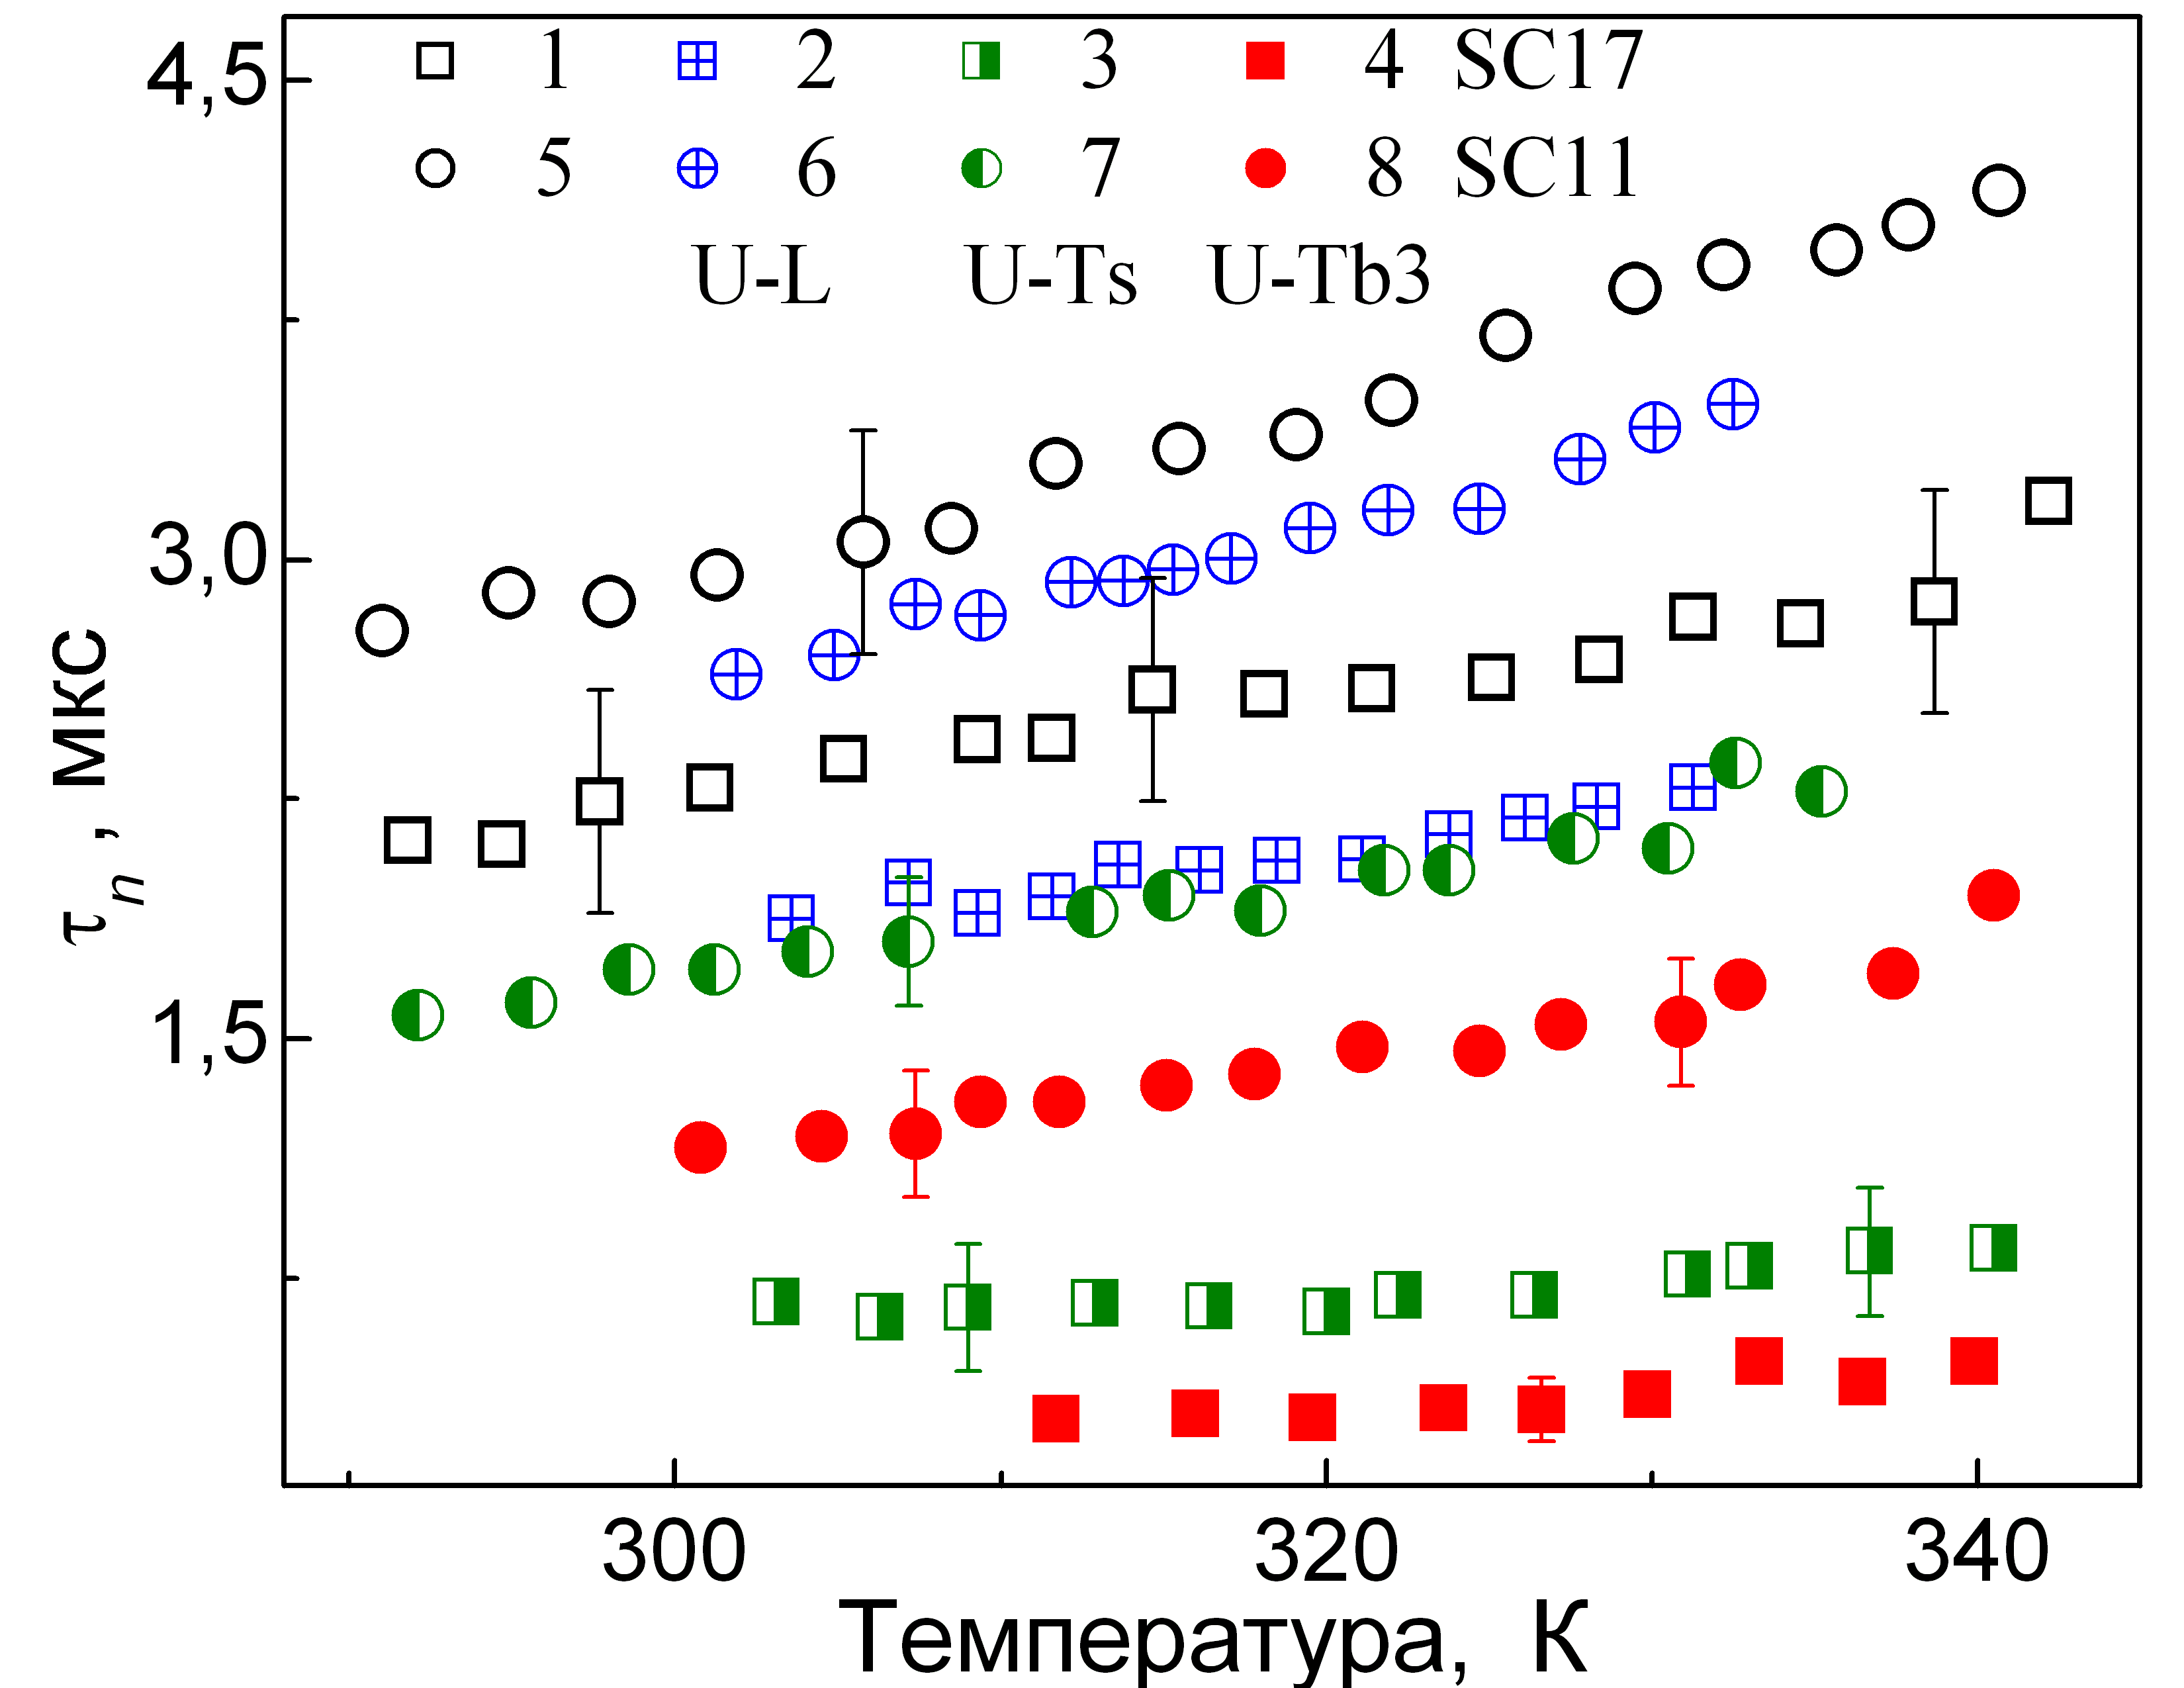
\includegraphics[width=0.7\textwidth]{figDUSTau}%
\caption{\label{figDUSTau}
Температурні залежності часу життя неосновних носіїв в КНО
для зразків SC17 (криві 1--4, квадрати) та SC11 (5--8, кола).
\FigCaptionSSC
}%
\end{figure}

Час життя неосновних носіїв в загальному випадку описується наступним чином \cite{MurphyJAP2011}:
\begin{equation}
\label{eqTAUsum}
\tau_n^{-1}=\tau_\mathtt{bb}^{-1}+\tau_\mathtt{CE\,Auger}^{-1}+\tau_\mathtt{SRH}^{-1}\,,
\end{equation}
де
$\tau_\mathtt{bb}$ --- час життя, пов'язаний з випромінювальною міжзонною рекомбінацією
\begin{equation}
\label{eqTAUbb}
\tau_\mathtt{bb}^{-1}=B(p_p+n_p+\Delta n)\,,
\end{equation}
$B$ --- коефіцієнт міжзонної рекомбінації, $B=1\cdot10^{-14}$~см$^3$c$^{-1}$ \cite{Si:TAUbb,MurphyJAP2011},
$\Delta n$ --- концентрація нерівноважних електронів,
$\tau_\mathtt{CE\,Auger}$ визначається Оже--рекомбінацією, підсиленою внаслідок кулонівської взаємодії  \cite{Si:TAUAuger}
\begin{equation}
\label{eqTAAuger}
\tau_\mathtt{CE\,Auger}=\frac{\Delta n}{np\left(1,8\cdot10^{-24}n_p^{0,65}+6\cdot10^{-25}p_p^{0,65}+3\cdot10{-27}\Delta n^{0.8}\right)}\,,
\end{equation}
$n$ та $p$ --- концентрації електронів та дірок, відповідно;
$\tau_\mathtt{SRH}$ --- час рекомбінації ШРХ.
В наших дослідах $\Delta n$ не перевищувала $8\cdot10^{13}$~см$^{-3}$.
Як наслідок, розрахунки показали, що $\tau_\mathtt{bb}^{-1}\leq14$~с$^{-1}$, $\tau_\mathtt{CE\,Auger}^{-1}\leq6$~с$^{-1}$.
А отже, міжзонною рекомбінацією та рекомбінацією Оже можна знехтувати, $\tau_n=\tau_\mathtt{SRH}$.

За умови низького рівня інжекції якщо в кристалі присутні декілька рекомбінаційних центрів $\tau_\mathtt{SRH}$ описується виразом

\begin{equation}
\label{eqTAUSHRsum}
\tau_n^{-1}=\sum_i^{M_d}\tau_{n,i}^{-1}=\sum_i^{M_d}N_{d,i}\,\sigma_{n,i}\,\upsilon_{\mathrm{th},n}\,,
\end{equation}
де
$M_d$ --- загальна кількість типів центрів,
$\tau_{n,i}$ описує час життя при рекомбінації лише за участю дефектів $i$--го типу,
які характеризуються концентрацією $N_{d,i}$ та ППЗ електронів $\sigma_{n,i}$.

На Рис.~\ref{figKus} наведено залежність оберненого часу життя в ОПЗ від параметрів УЗН,
причому в одному випадку таким параметром вибрана $W_{U\!S}$, а в другому ---$u_\mathtt{US}^2$.
Видно, що $\tau_n^{-1}$ лінійно зростає з підвищенням інтенсивності введеного УЗ,
тобто АІ зміни часу життя можна записати у вигляді

\begin{figure}
\center
%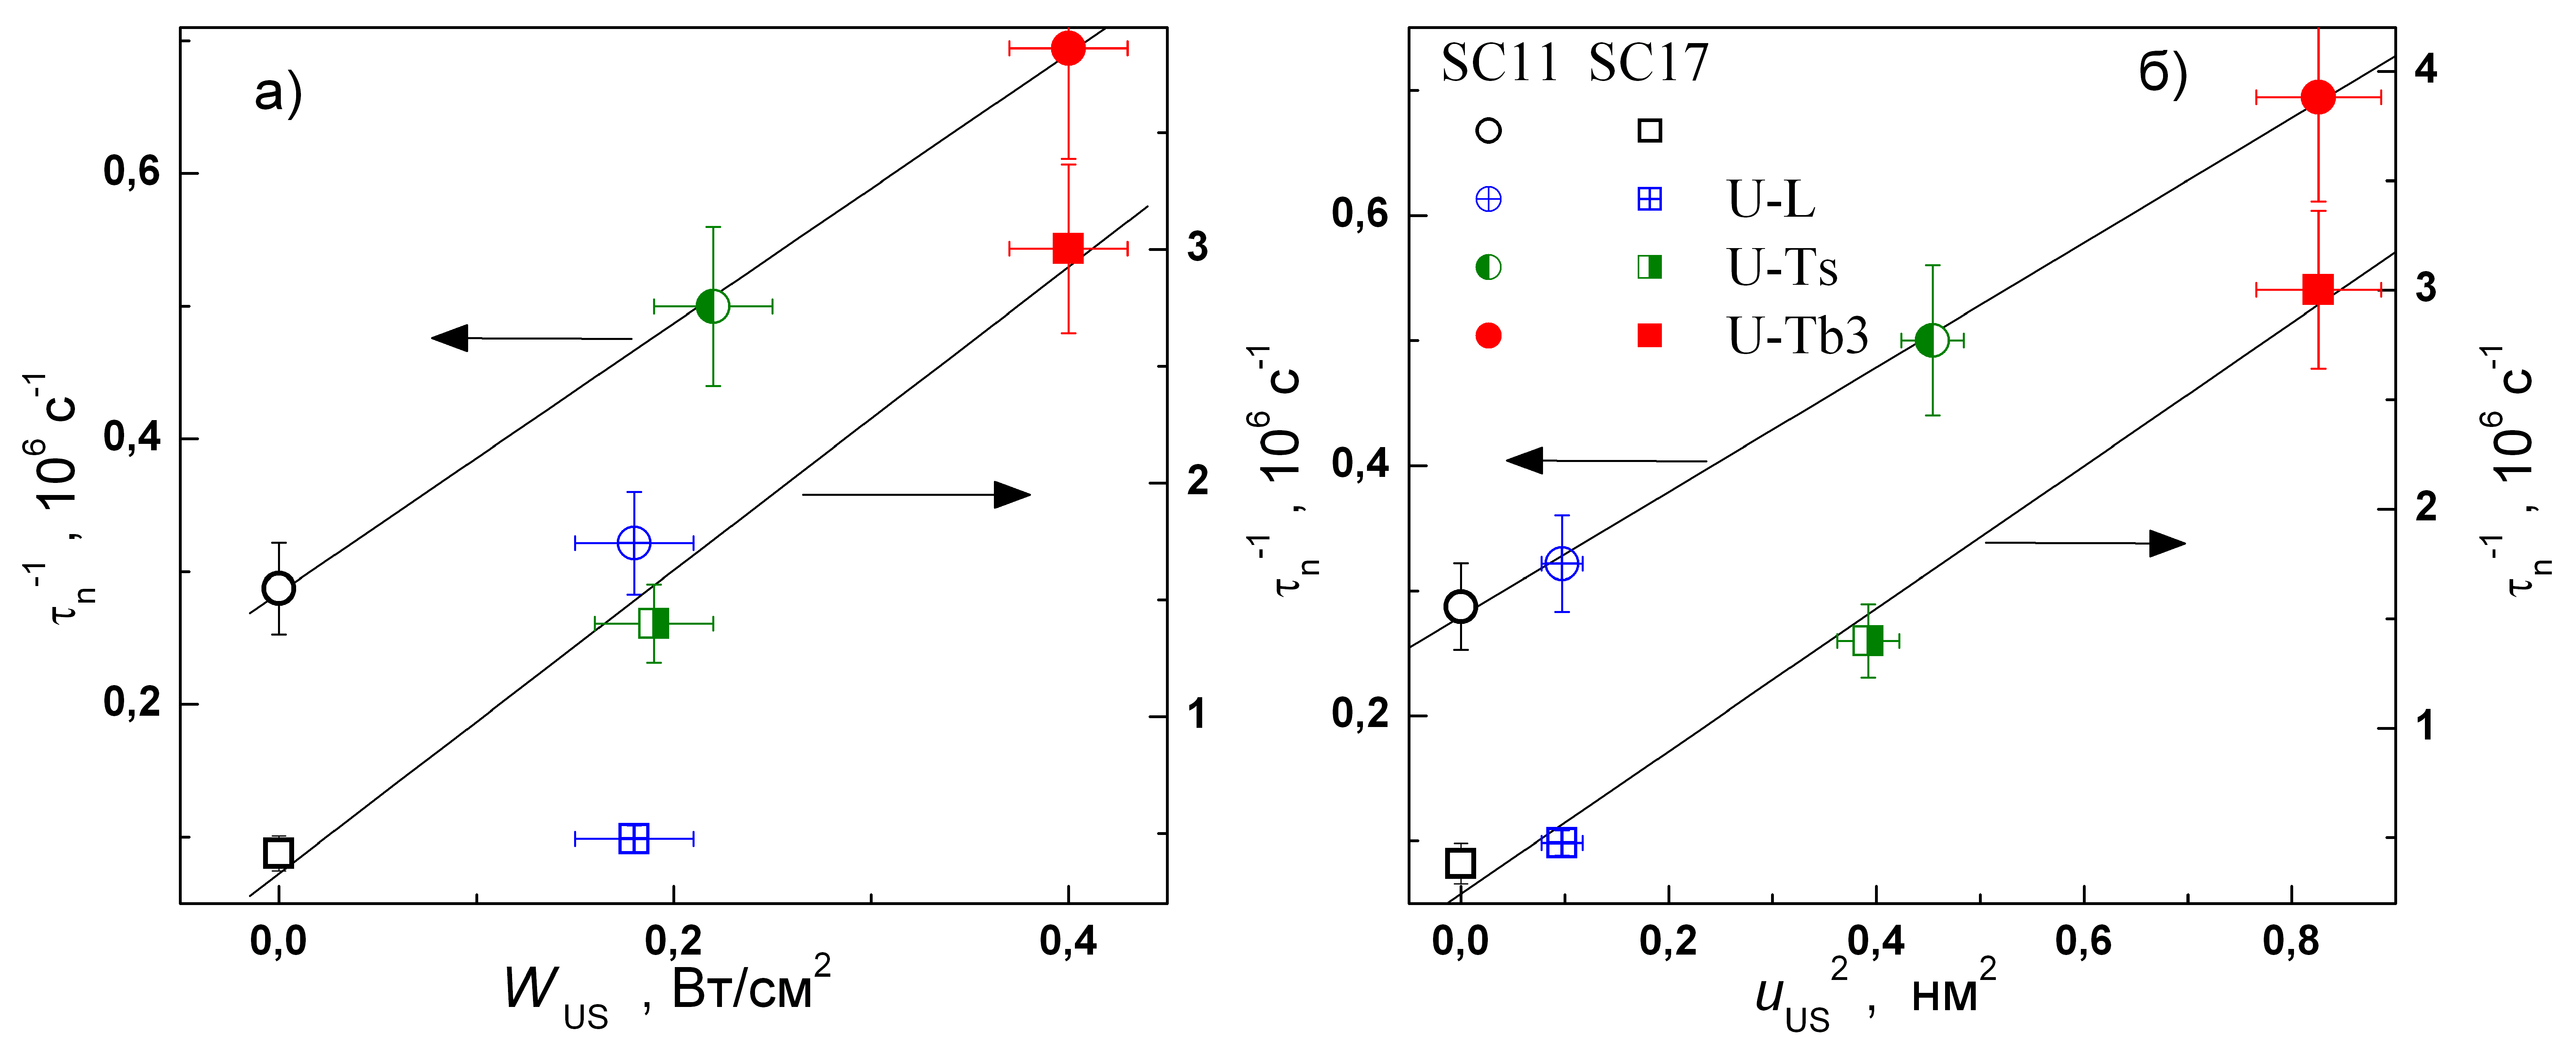
\includegraphics[width=1\textwidth]{figKus}%
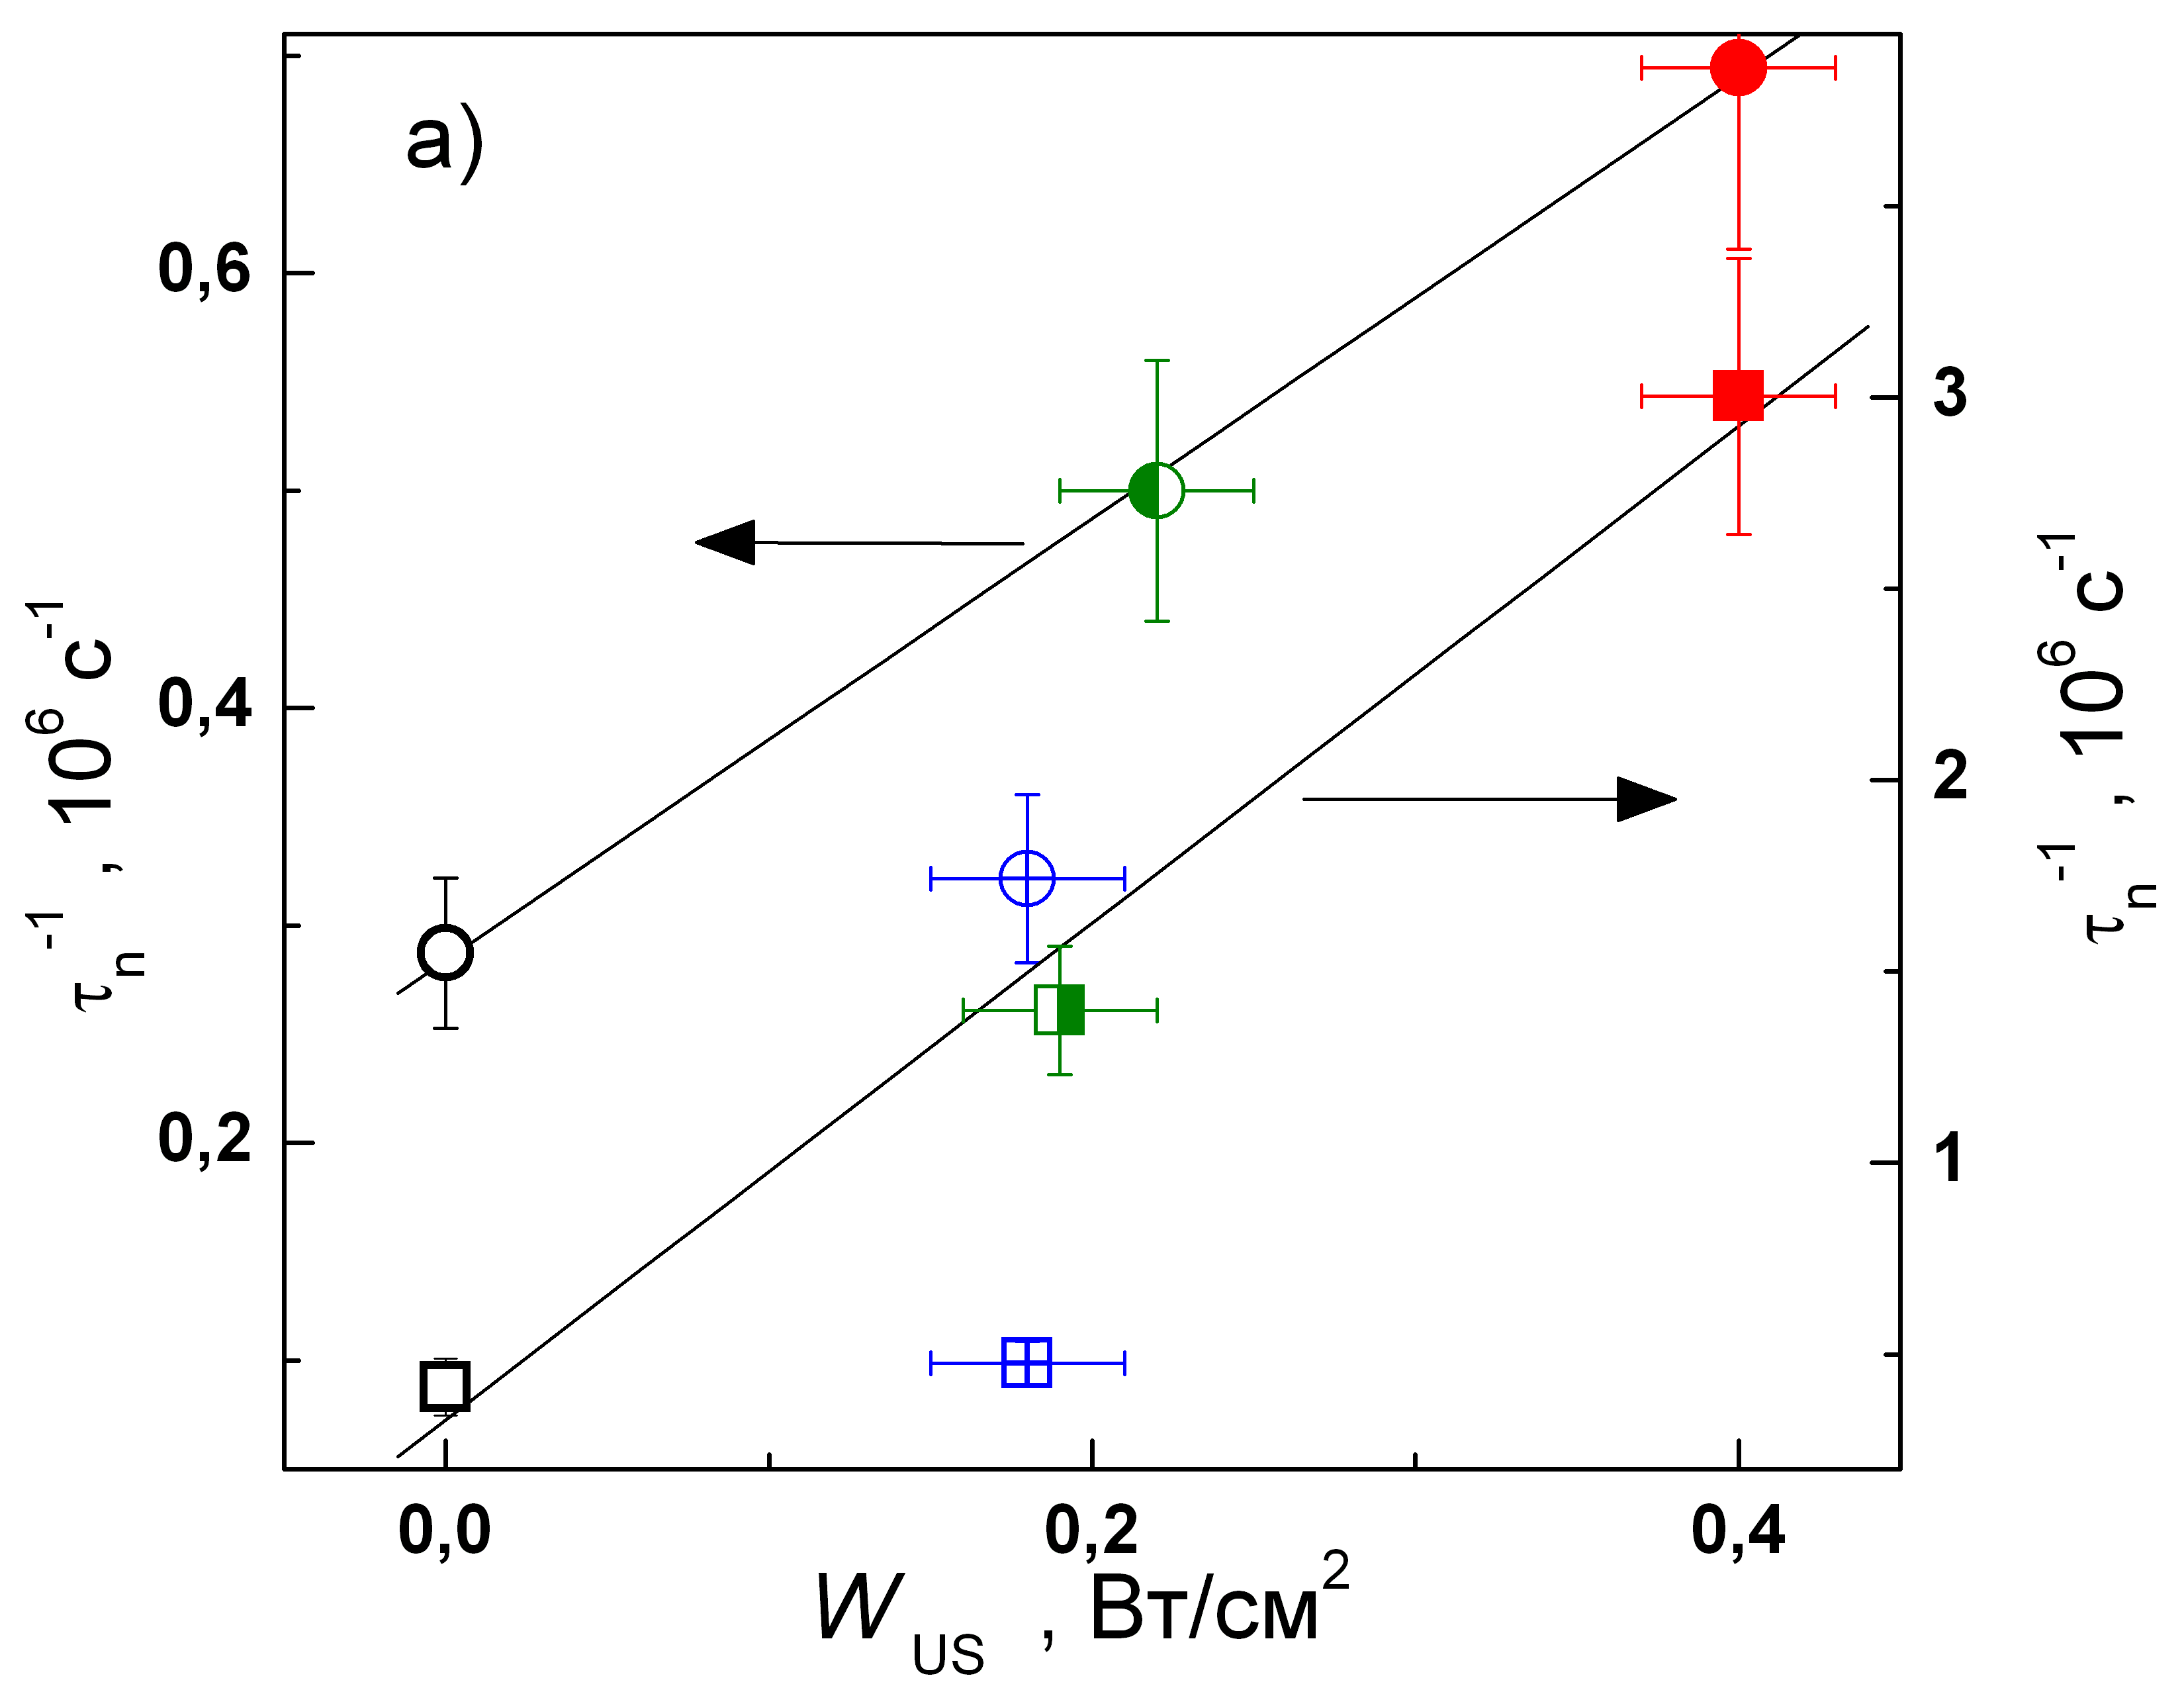
\includegraphics[width=0.49\textwidth]{figKus_a} \hfill
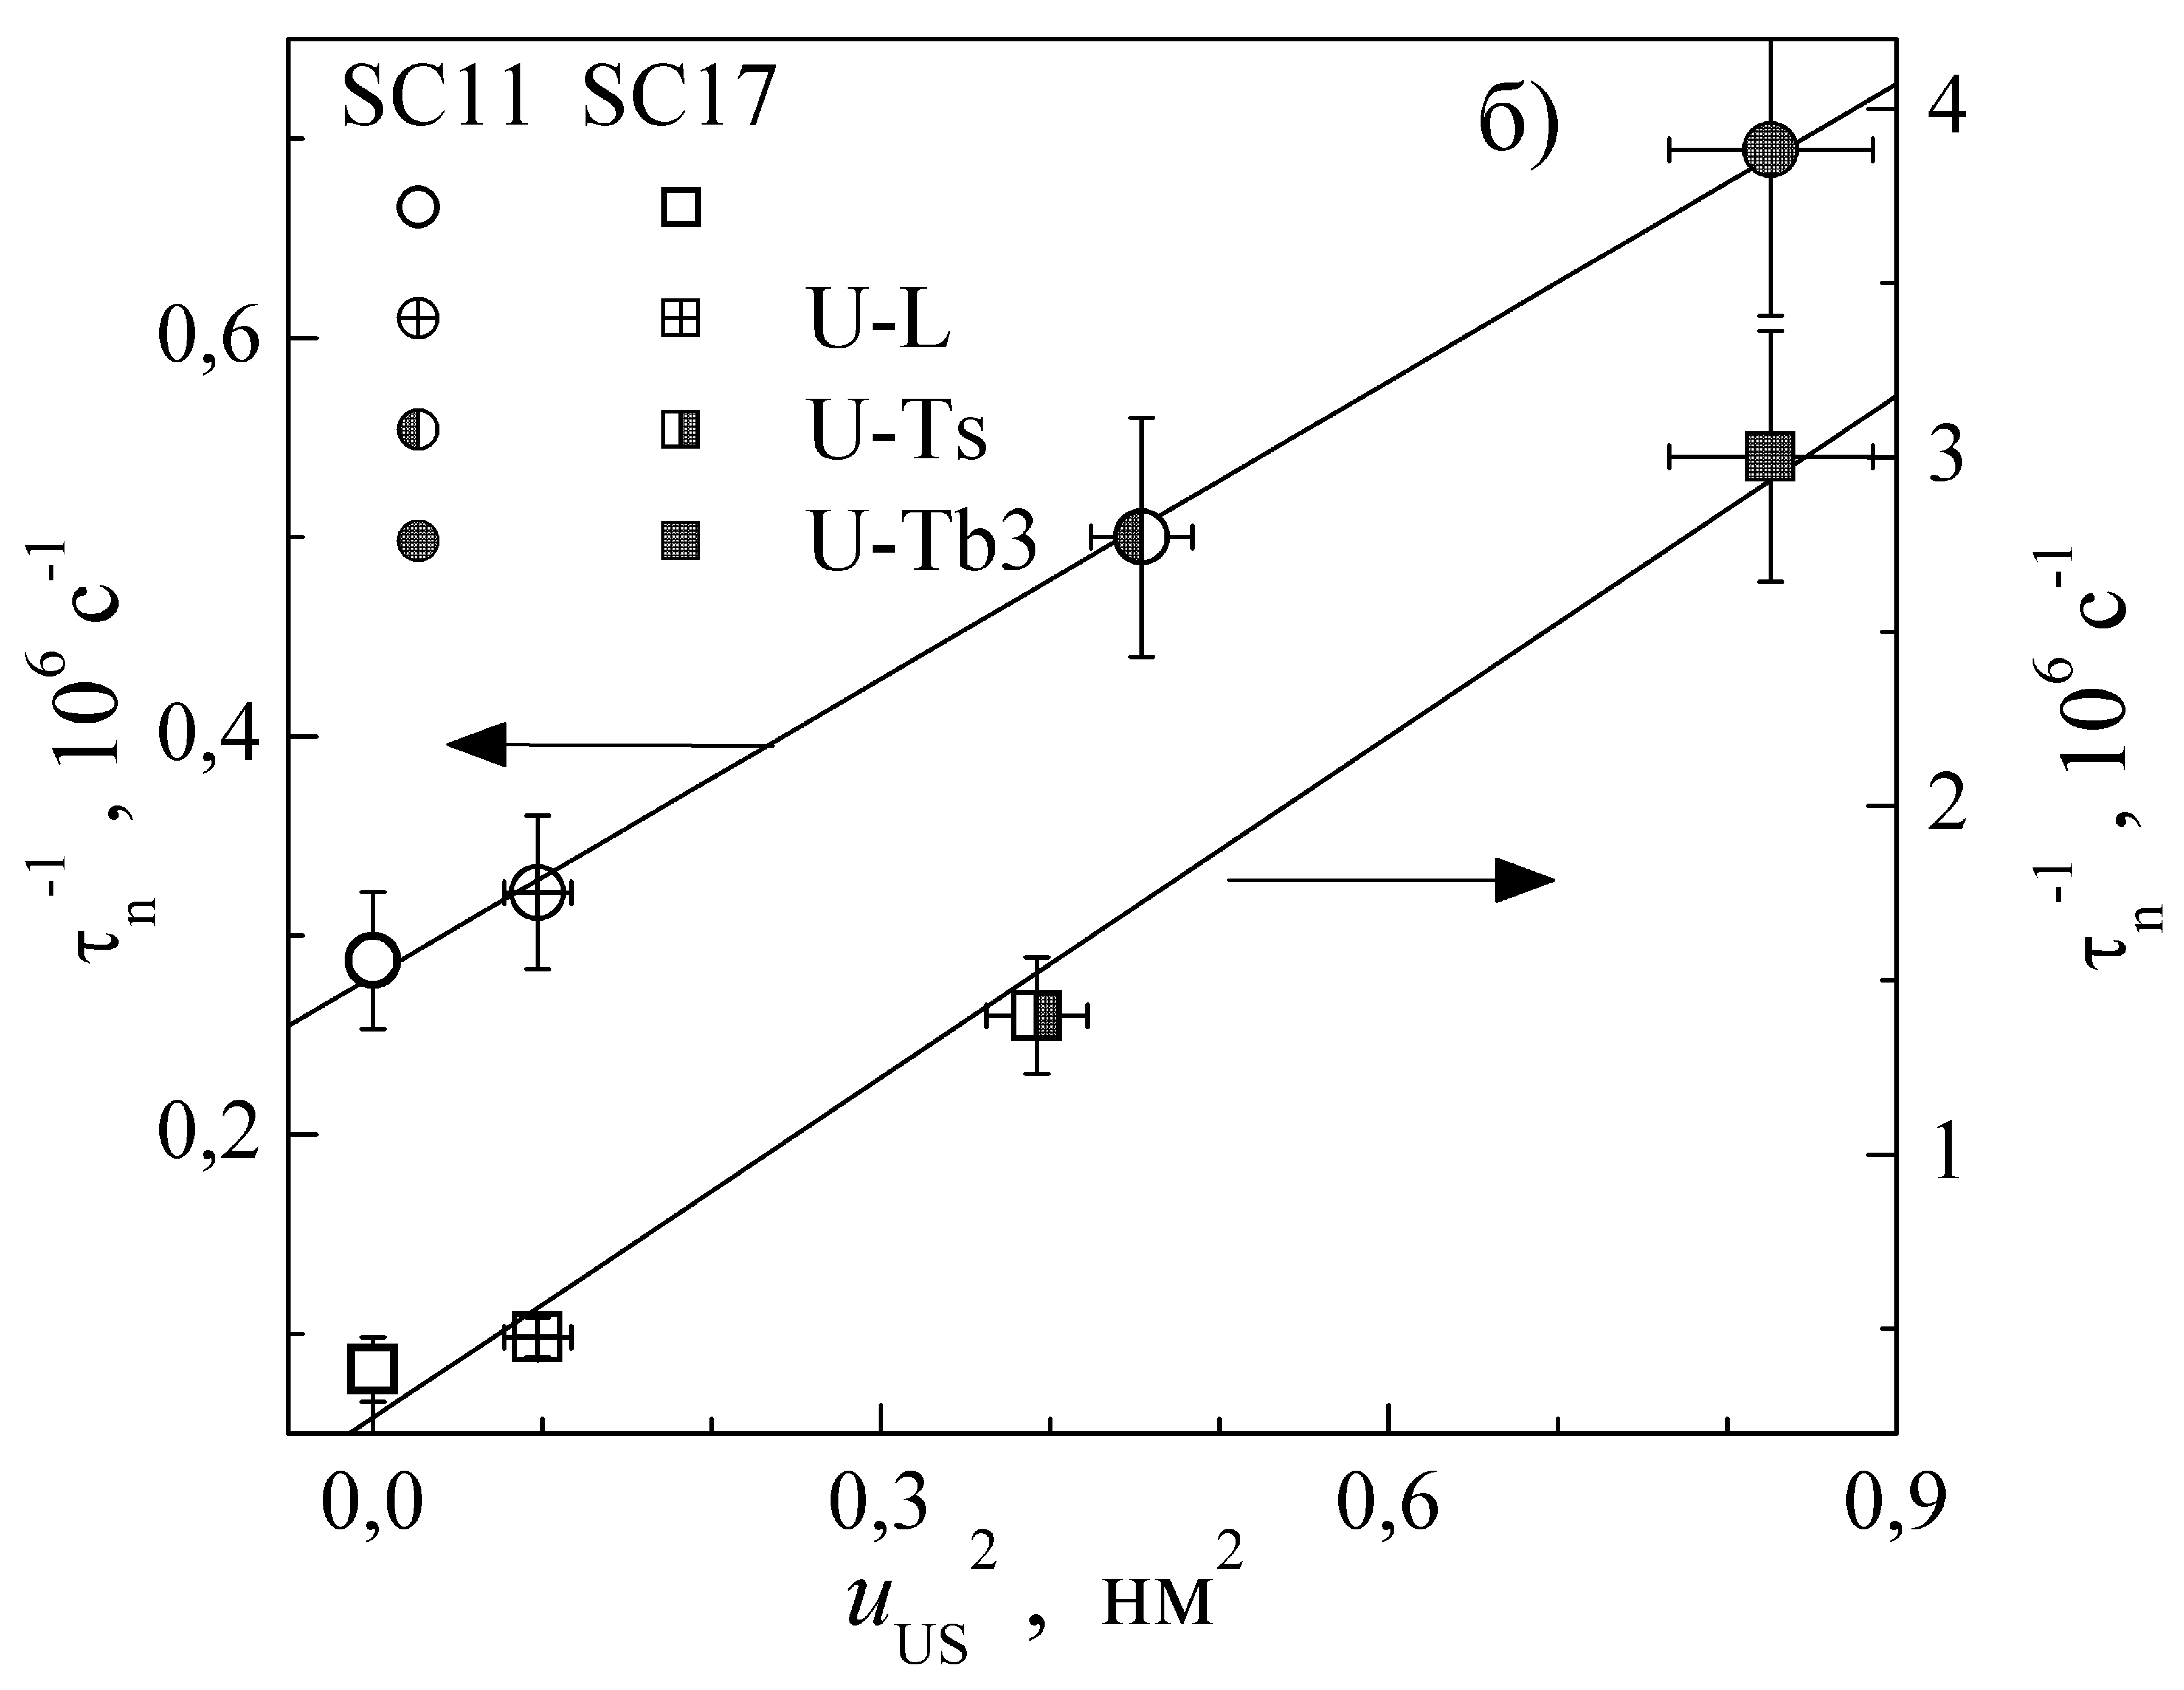
\includegraphics[width=0.49\textwidth]{figKus_b}
\caption{\label{figKus}
Залежність оберненого часу життя в ОПЗ від інтенсивності введеного звуку (а)
та від квадрату амплітуди АІ зміщень атомів для SC17 (квадрати, праві осі обох графіків)
та SCR11 (кола, ліві осі) при 320~K.
Заповнення точок залежить від УЗН і збігається з наведеним на Рис.~\ref{figDUSTau}.
Прямі - лінійна апроксимація (для а - лише даних, отриманих при використанні поперечних хвиль.
}%
\end{figure}

\begin{equation}
\label{eqMS_UsW}
\tau_n^{-1}=\tau_{n,in}^{-1}+K_\mathtt{US}^{*}\,W_\mathtt{US}\,,
\end{equation}
або
\begin{equation}
\label{eqMS_Us}
\tau_{n,\mathtt{US}}^{-1}=\tau_{n,in}^{-1}+K_\mathtt{US}\,u_\mathtt{US}^2 \,,
\end{equation}
де $K_\mathtt{US}^{*}$ та $K_\mathtt{US}$ характеризують акусто--дефектну взаємодію (АДВ) і залежать від властивостей дефекту та характеристик кристалу.
Проте використання  другого виразу є більш доцільним, так як $K_\mathtt{US}^{*}$ залежить також і від типу збуджених хвиль,
тоді як $K_\mathtt{US}$ визначається лише АДВ.
Іншими словами, саме зміщення атомів (а не інтенсивність АХ) є основним фактором впливу УЗН на рекомбінацію носіїв заряду.
Зауважимо, що вирази (\ref{eqMS_UsW}) та (\ref{eqMS_Us}) за формую схожі з добре відомою формулою Messenger–-Spratt \cite{Markvart},
яка описує зміни часу життя внаслідок радіаційного опромінення, причому роль флюєнса відіграє $u_\mathtt{US}^2$ ($W_\mathtt{US}$).

Визначені величини $K_\mathtt{US}$ наведено в Таблиці~\ref{tabSSCParam}.

\begin{figure}
\center
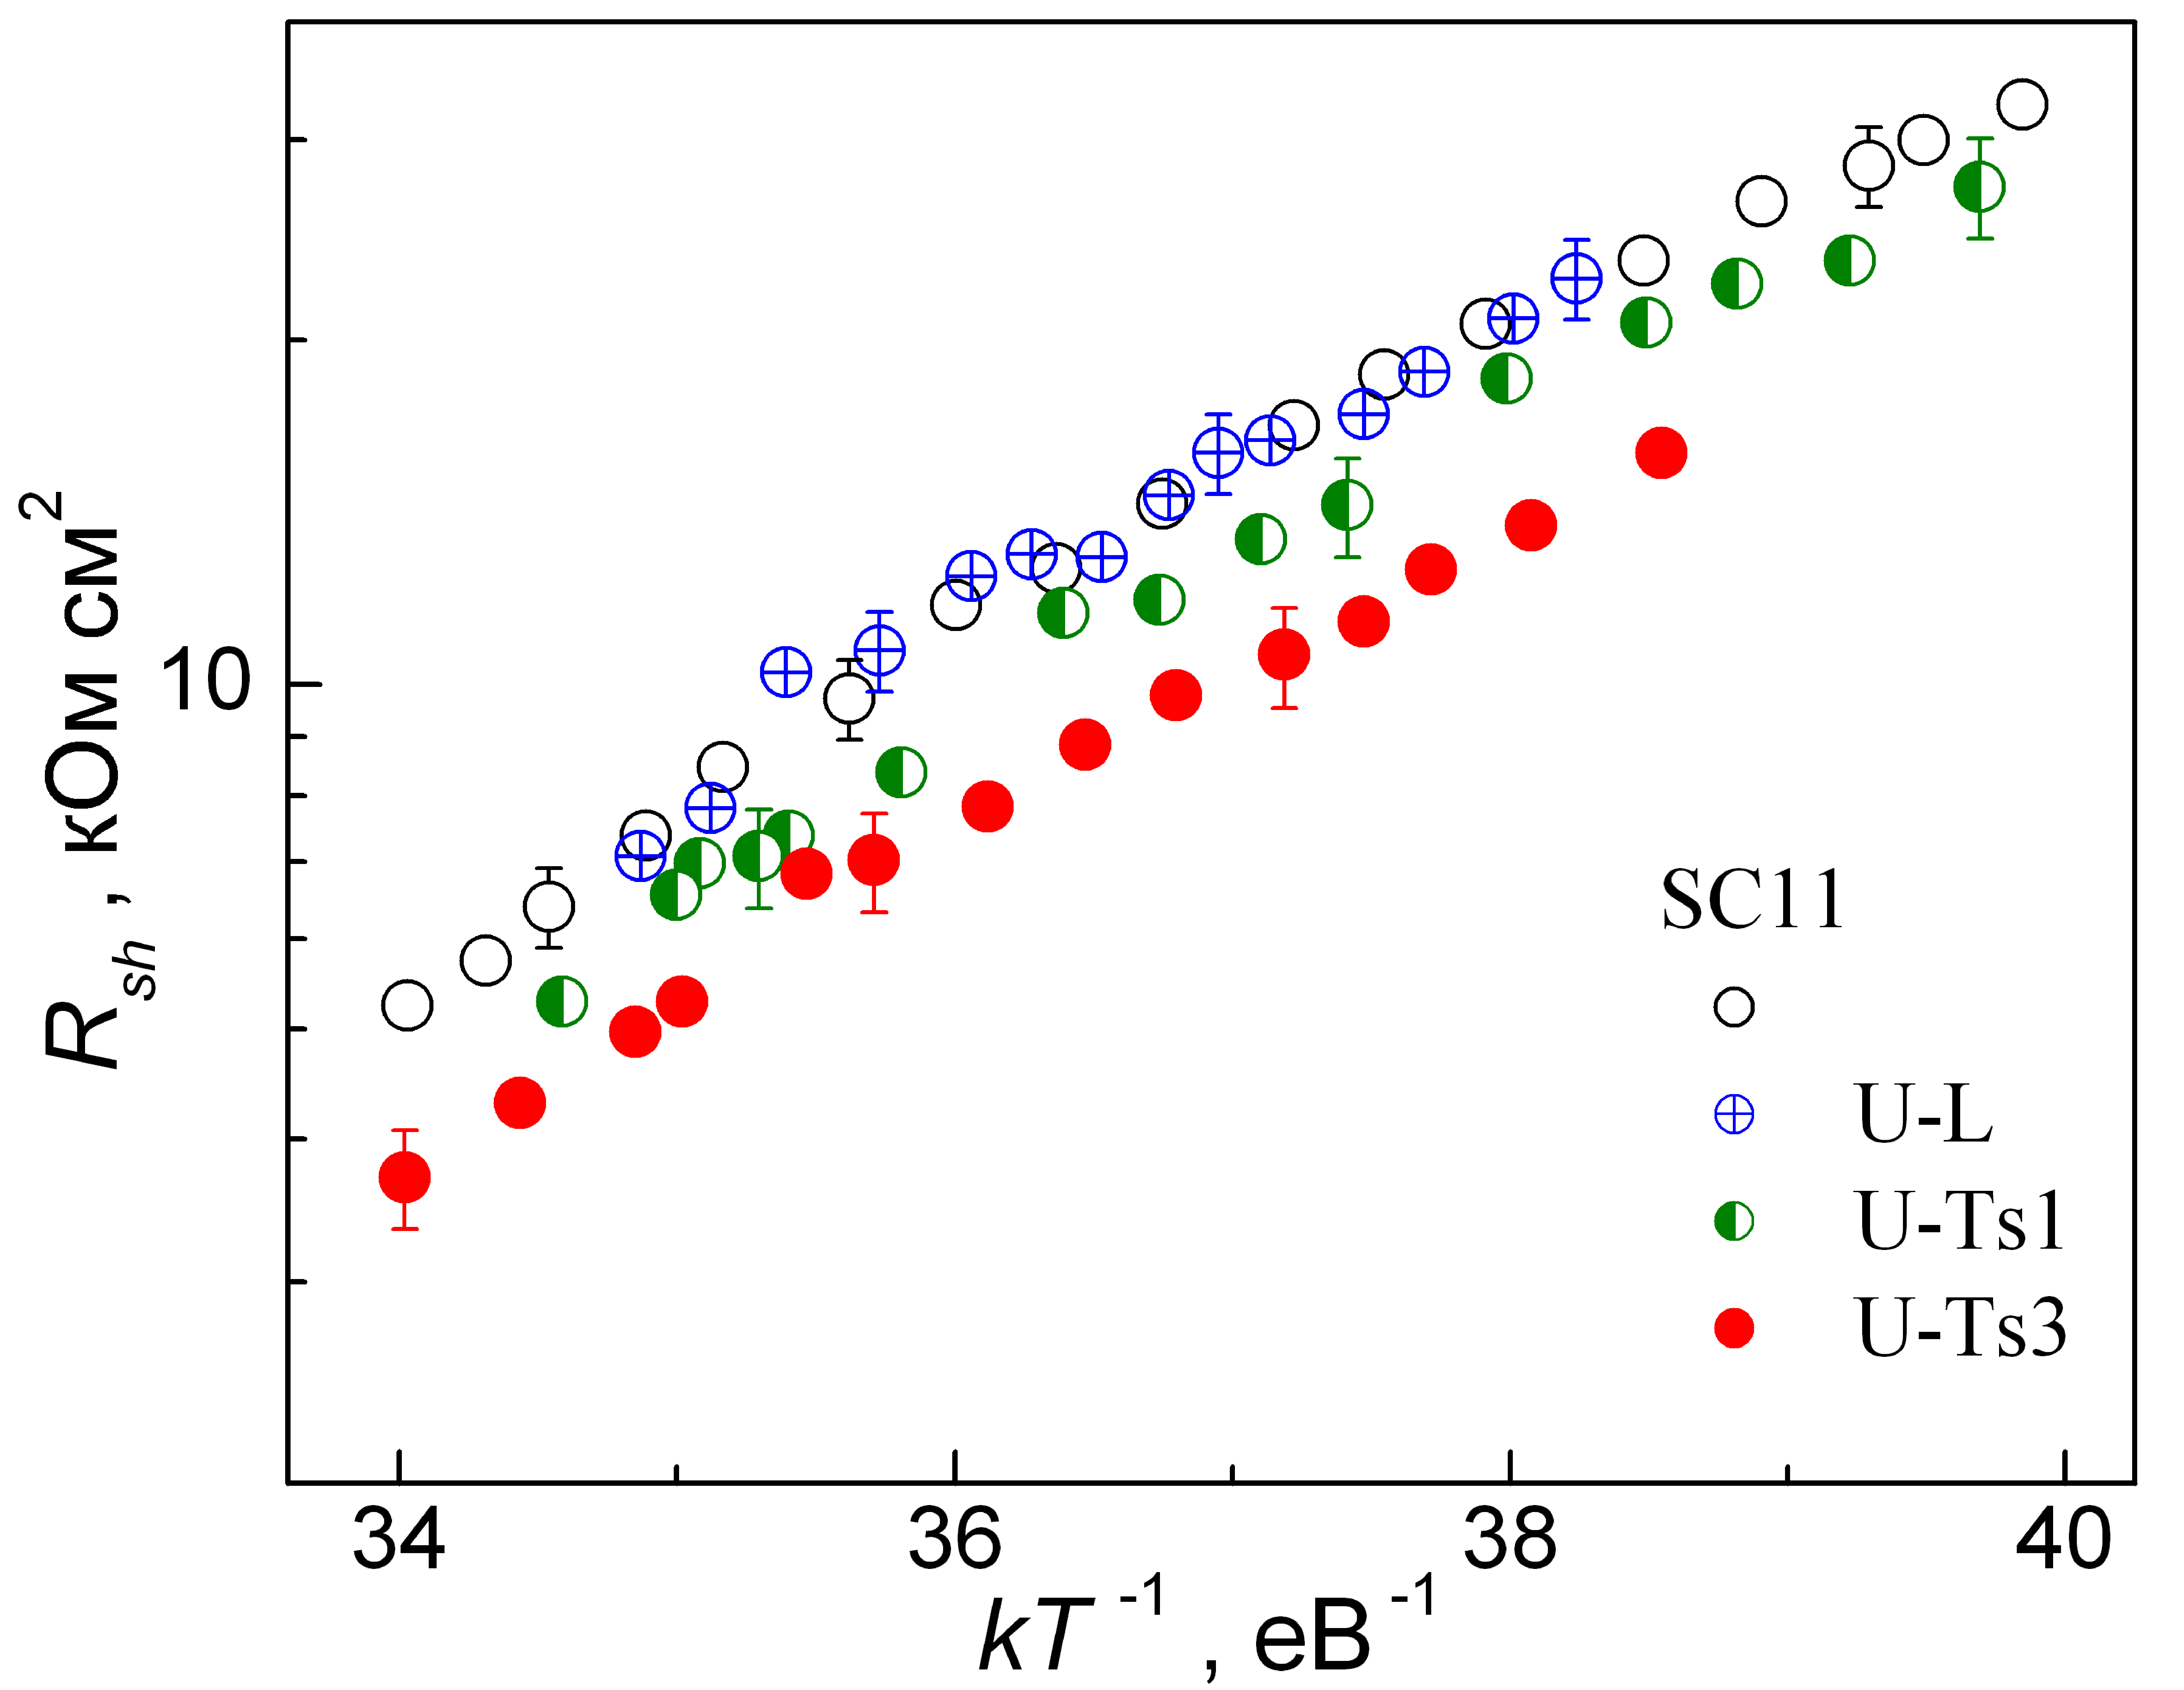
\includegraphics[width=0.7\textwidth]{figDUS_Rsh}%
\caption{\label{figDUS_Rsh}
Температурні залежності шунтуючого опору SC11, отримані за умов УЗН та без нього (порожні кола).
}%
\end{figure}

На Рис.~\ref{figDUS_Rsh} показана температурна залежність шунтуючого опору зразка SC11.
Зауважимо, що для SC17 $R_{sh}>10^{15}$~Ом$\cdot$см$^2$ незалежно від температури та УЗН і
шунтуючий опір не впливав на ВАХ.
З усього дослідженого набору зразків лише цей мав подібну особливість.
З рисунка видно, що УЗН з використанням поперечних хвиль викликає зменшення $R_{sh}$,
тоді як повздовжні хвилі практично не впливають на величину шунтуючого опору.
Розраховані величини як $R_{sh}$, так і його АІ змін наведені в Таблицях~\ref{tabSSCParam} та \ref{tabAIEfect}.
Детальний розгляд можливих причин виникнення $R_{sh}$ та впливу на нього УЗН наведено у параграфі~\ref{sbRsh}.

\subsection{Модель акусто--активного комплексного дефекту\label{sbAEDefect}}

Для пояснення взаємодії пружних хвиль з дефектами у неп'єзоелектричних кристалах
запропоновано чимало механізмів.
Зокрема вважається, що в умовах УЗН може відбуватися
\begin{enumerate}[label=\asbuk*),leftmargin=0em,itemindent=1.5em]
\item зміна заселеності коливних рівнів, зв'язаних з домішками \cite{Pavlovich};
\item зміщення домішкових атомів порівняно з їх оточенням \cite{Korotchenkov1995,MirzadeJAP2011,PELESHCHAK:UPJ2016};
\item зменшення енергії активації дифузії дефектів \cite{Krevchik};
\item локальне підвищення температури в області кластерів точкових дефектів  \cite{MirzadeJAP2005};
\item поглинання УЗ дислокаціями \cite{Davletova2008,OstrovKor92};
\end{enumerate}
тощо.
Проте повна теорія АДВ в кремнії ще не побудована, причиною чого, зокрема, є недостатня
кількість експериментальних досліджень, сфокусованих на вивчення АІ ефектів.

На нашу думку, виявлені оборотні АІ зміни рекомбінаційних параметрів КСЕ можна пояснити зміною
відстані між компонентами дефектного комплексу в умовах УЗН.
Зокрема, якщо мова йде про АІ модифікацію $n_{\mathrm{id}}$ та $\tau_g$,
то відбувається зміна відстані між донором та акцептором, які приймають участь у CDLR.

Дійсно, з літератури \cite{MirzadeJAP2011,PELESHCHAK:UPJ2016} відомо, що для сили $F_d$, яка діє на точковий дефект під час УЗН,
є справедливим вираз
\begin{equation}
\label{eqFd}
F_d=\chi\,\Delta\Omega_d\frac{\partial \xi(z,t)}{\partial z}\,,
\end{equation}
де
$\chi$ --- об'ємний модуль пружності,
$\Delta\Omega_d$ --- зміна об'єму кристалу, що припадає на один дефект
(для міжвузлових атомів та домішок заміщення з іонним радіусом, що перевищує радіус атома матриці $\Delta\Omega_d > 0$,
тоді як для вакансій та домішок заміщення з меншим іонним радіусом $\Delta\Omega_d < 0$);
$\xi$ --- деформація кристалічної ґратки;
при цьому вважається, що АХ поширюється в напрямі осі $Z$;
$\partial \xi(z,t)/\partial z\sim \xi_{\mathtt{US}}\sim u_\mathtt{US} \sim \sqrt{W_\mathtt{US}}$.
Таким чином, під час УЗН точковий дефект здійснює коливання, причому їх амплітуда та фаза визначаються як параметрами самого ТД, так і інтенсивністю АХ.


\begin{figure}
\center
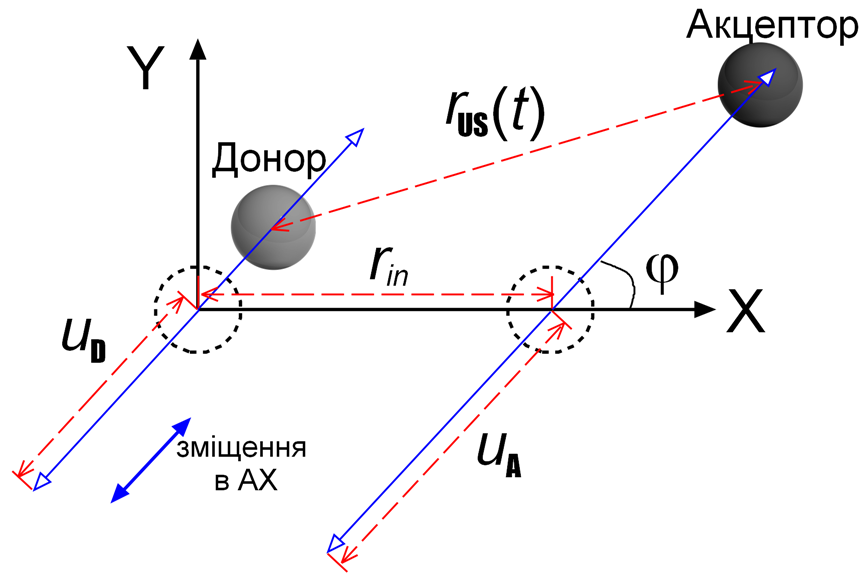
\includegraphics[width=0.7\textwidth]{fig_Model}
\caption{\label{fig_Model}
Модель поведінки дефектного комплексу в умовах УЗН.
}%
\end{figure}

На Рис.~\ref{fig_Model} показана спрощена якісна модель поведінки дефектного комплексу, який містить дві складові,
в умовах поширення АХ.
У вихідному стані, до УЗН, донор та акцептор перебувають на відстані $r_{in}$ один від одного,
вісь $X$ спрямована вздовж прямої, яка з'єднує дефекти.
В умовах УЗН дефекти коливаються з амплітудами $u_\mathtt{D}$ та $u_\mathtt{A}$.
Напрям коливань збігається з напрямом зміщень в АХ та утворює кут $\varphi$ з віссю $X$.
$u_\mathtt{D}$ та $u_\mathtt{A}$ залежать від $\xi_{U\!S}$, пружних полів дефекту (значень $\Delta\Omega_d^\mathtt{D}$ та $\Delta\Omega_d^\mathtt{A}$,
пов'язаних з кожною окремою складовою), енергії зв'язку комплексу і можуть відрізнятися між собою.
Відповідно, відстань між донором та акцептором за умов УЗН залежить від часу $t$:
\begin{multline}
\label{eqrUS}
r_\mathtt{US}(t)=\left\{[r_{in}+u_\mathtt{A}\cos(\omega_\mathtt{US}t+\delta)-u_\mathtt{D}\cos(\omega_\mathtt{US}t)]^2\cos^2\varphi \right.\\
    \left.+ [u_\mathtt{A}\cos(\omega_\mathtt{US}t+\delta)-u_\mathtt{D}\cos(\omega_\mathtt{US}t)]^2\sin^2\varphi\right\}^{0.5}\,,
\end{multline}
де
$\omega_\mathtt{US}$ --- циклічна частота УЗ, а
$\delta$ --- зсув фаз між коливаннями донора та акцептора.

Зміна відстані між компонентами комплексу, згідно з моделлю CDLR, має викликати зміни
ППЗ носіїв та величини $R_\mathtt{DA}$.
Використовуючи формули (\ref{eqSigma}) and (\ref{eqRda}), були проведені розрахунки
АІ відносних змін поперечного перерізу захоплення
$\varepsilon_\sigma=[\sigma_{\mathtt{US}}-\sigma(r_{in})]/\sigma(r_{in})$
та параметру зв'язку
$\varepsilon_{\mathtt{RDA}}=[R_{\mathtt{DA,US}}-R_\mathtt{DA}(r_{in})]/R_\mathtt{DA}(r_{in})$,
де $\sigma_{\mathtt{US}}$ та $R_{\mathtt{DA,US}}$ були усереднені по періоду АХ $T_\mathtt{US}$:
\begin{equation}
\label{eqAverSigma}
\sigma_{\mathtt{US}}=\frac{1}{T_\mathtt{US}}\int^{T_\mathtt{US}}_0\!\!\!\!\!\!\sigma(r_\mathtt{US}(t))dt\,,
\end{equation}
\begin{equation}
\label{eqAverRda}
R_{\mathtt{DA,US}}=\frac{1}{T_\mathtt{US}}\int^{T_\mathtt{US}}_0\!\!\!\!\!\!R_{\mathtt{DA}}(r_\mathtt{US}(t))dt\,.
\end{equation}


\begin{figure}
\center
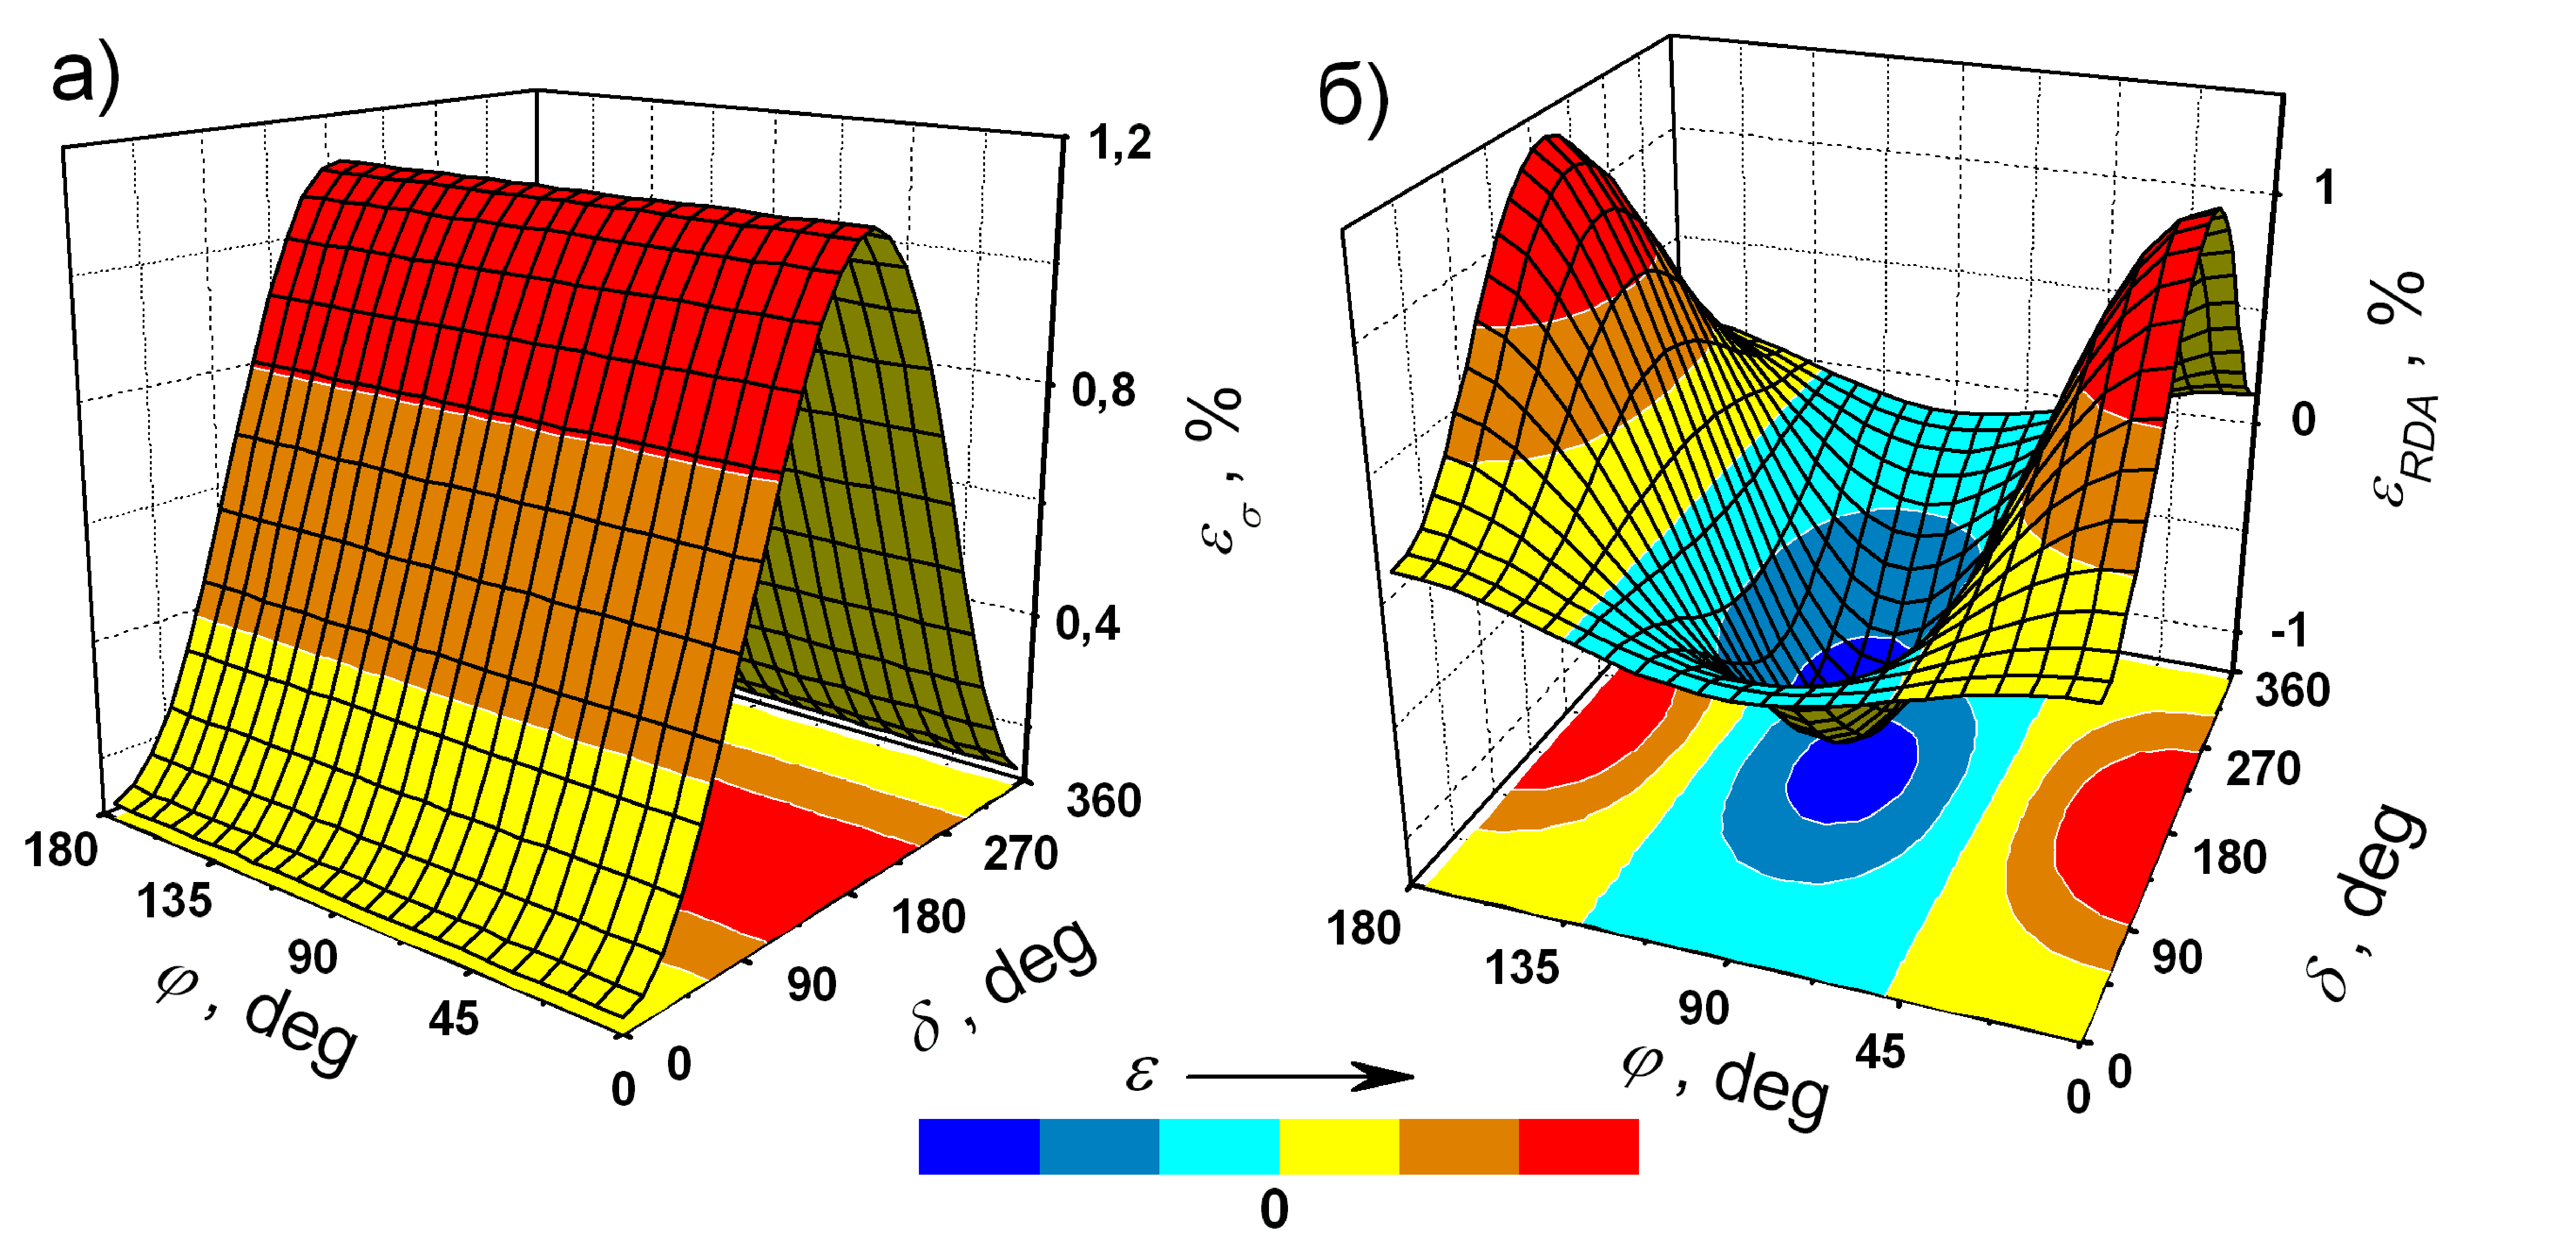
\includegraphics[width=0.95\textwidth]{figR2L}
\caption{\label{figR2L}
Розраховані залежності  АІ змін поперечного перерізу захоплення носіїв (а) та параметру зв'язку (б) від зсуву фаз між коливаннями та від взаємного
розташування вісі комплексу та напряму зміщень в АХ.
При розрахунках вважалося, що $a_B=3.23$~нм, $r_{in}=10$~нм, $u_A=1$~нм та $u_D=0.5$~нм.
}%
\end{figure}

\begin{figure}
\center
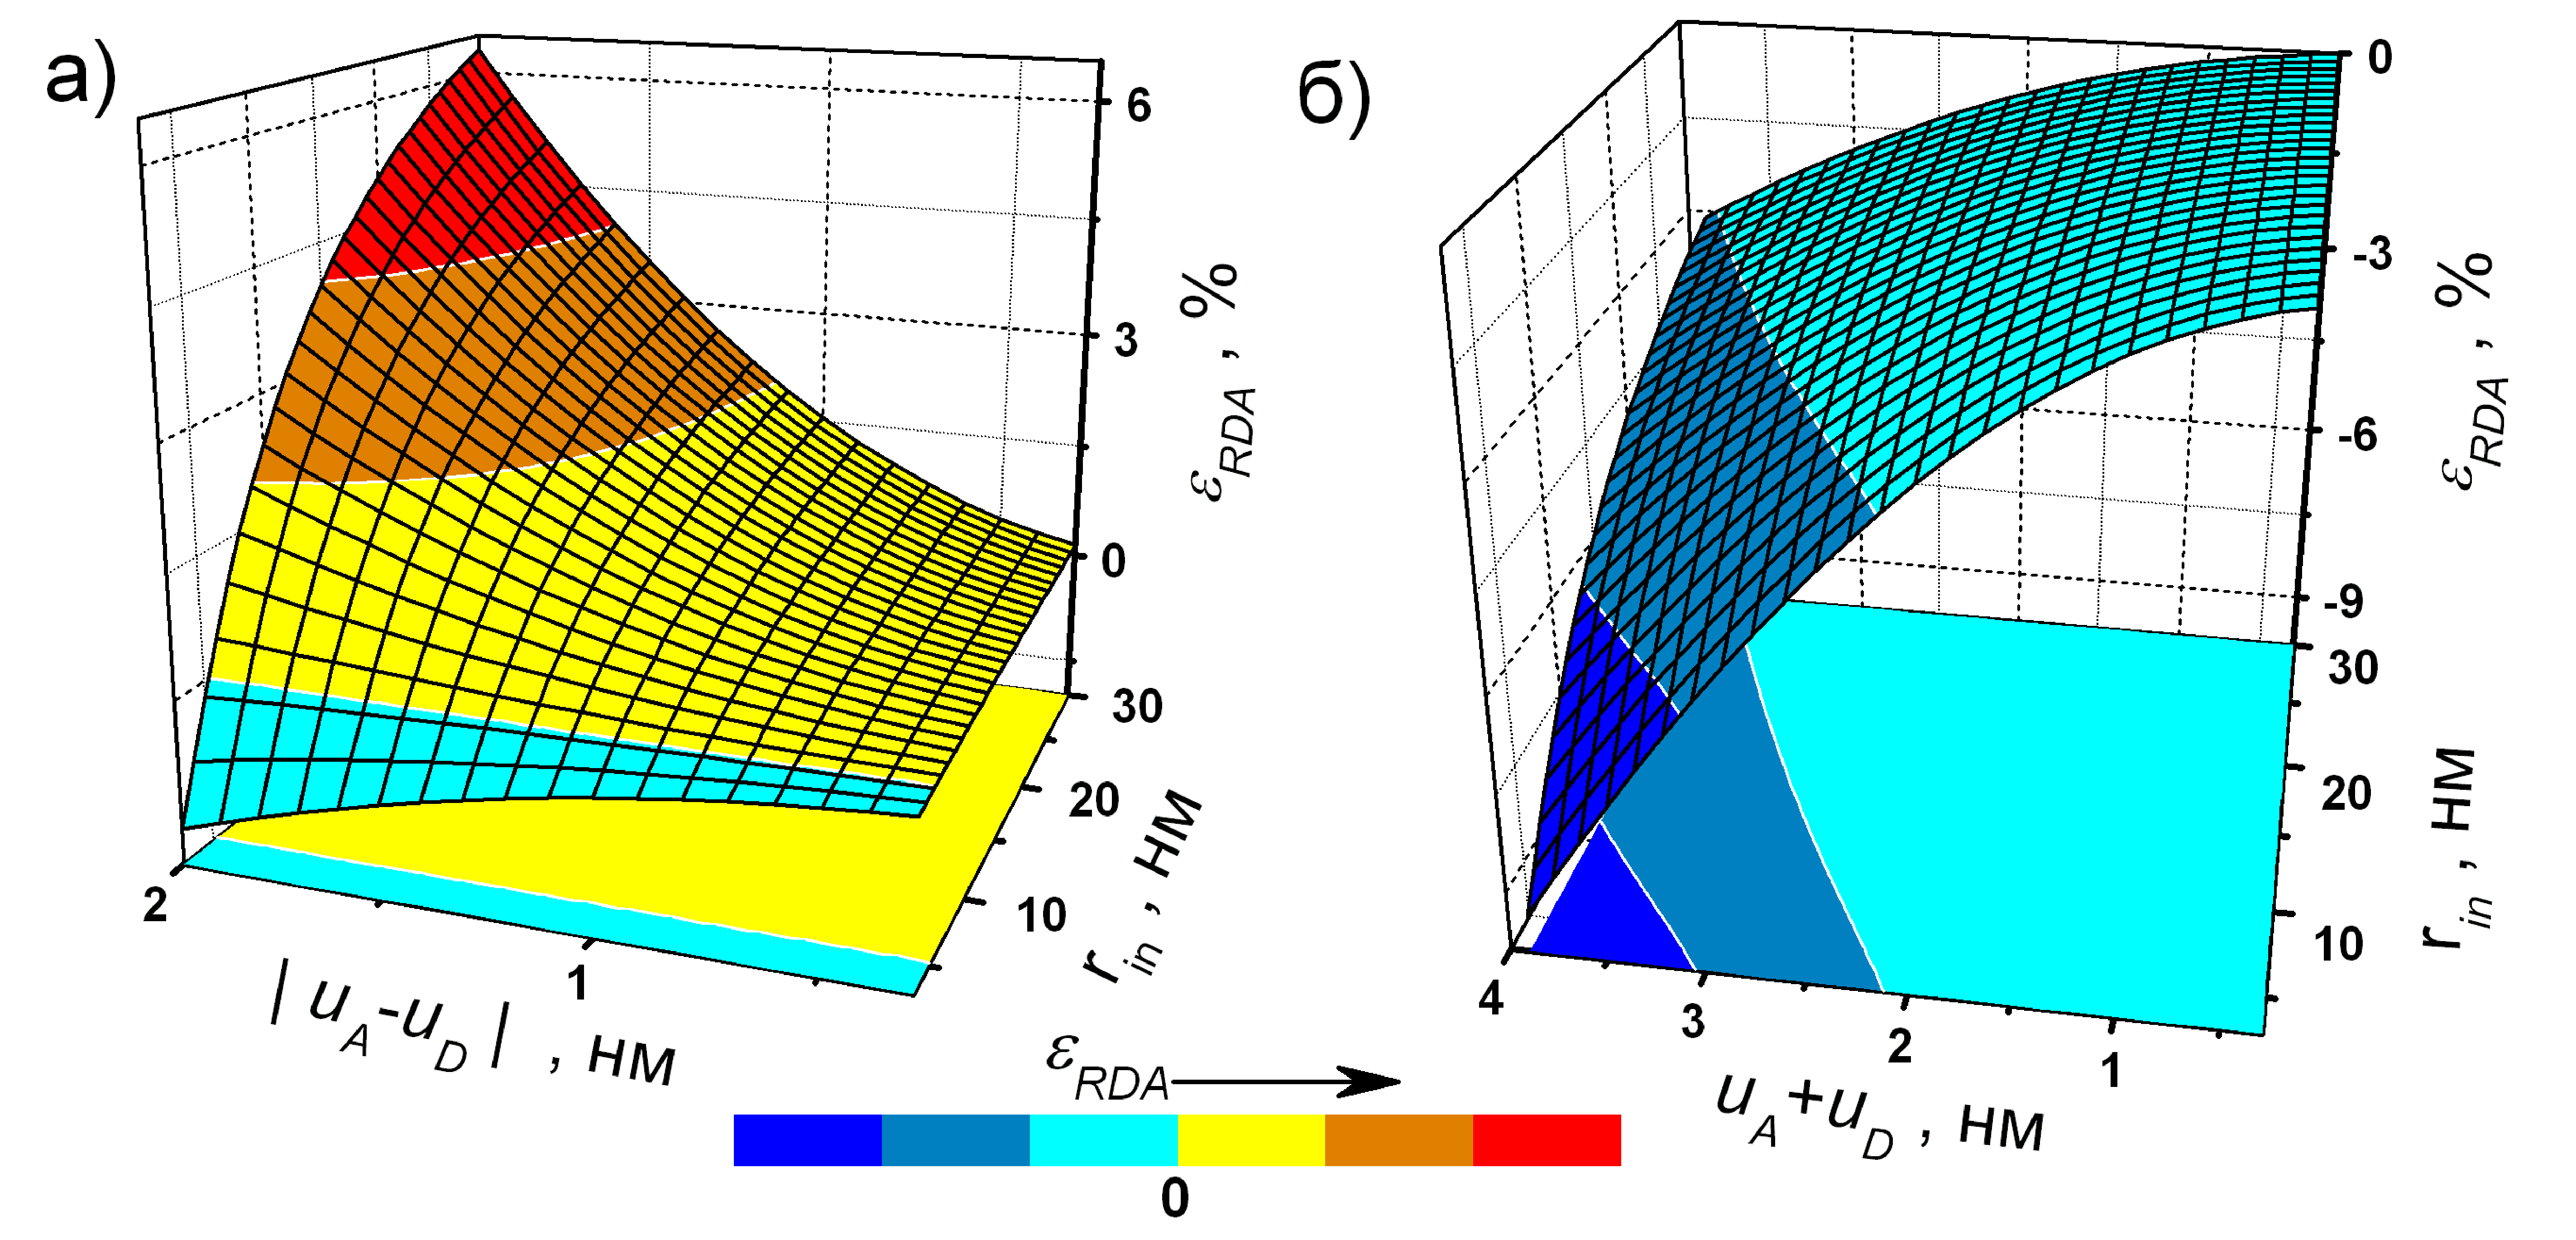
\includegraphics[width=0.95\textwidth]{figLnew}
\caption{\label{figLnew}
Розраховані залежності  АІ змін параметру зв'язку від амплітуди коливань та початкової відстані між компонентами.
При розрахунках вважалося, що $\varphi=0^\circ$, $\delta=0^\circ$ (a) та $\varphi=90^\circ$, $\delta=180^\circ$ (б).
}%
\end{figure}

Декілька типових прикладів результатів розрахунків показано на Рис.~\ref{figR2L} та Рис.~\ref{figLnew}.
Під час їх проведення вважалося, що
\begin{enumerate}[label=\asbuk*),leftmargin=0em,itemindent=1.5em]
\item характерний час релаксації в CDLR--підсистемі набагато менший, ніж $T_\mathtt{US}$;
\item $a_B=3.23$~нм ---значення, яке раніше використовувалося в літературі \cite{CDLR:JAP};
\item значення $u_\mathtt{D}$ та $u_\mathtt{A}$ співрозмірні з $u_\mathtt{US}$;
   проте при цьому потрібно взяти до уваги, що зміщення домішкових атомів, які не утворюють ковалентних зв'язків з оточенням, може перевищувати
   зміщення атомів, які утворюють кристалічну ґратку.
\end{enumerate}

Як видно з Рис.~\ref{figR2L},a, УЗН викликає збільшення ППЗ.
Залежності АІ змін параметру зв'язку більш складні і не монотонні -- див. Рис.Fig.~\ref{figR2L},б.
Зокрема, очікується  зменшення $R_{\mathtt{DA}}$ якщо $\varphi\approx90^\circ$ (тобто вісь комплексу перпендикулярна до напрямку зміщень в АХ, див. Рис.~\ref{figLnew},б)
або при малих значеннях $r_{in}/a_B$ (див. Рис.~\ref{figLnew},а).
До речі, в останньому випадку передбачається \cite{CDLR:JAP1995,CDLR:JAP}, що процеси CDLR будуть відбуватися найбільш інтенсивно.

Якщо припустити, що на дефектах не відбувається дисипація енергії УЗ, то в такому спрощеному випадку
$\delta$ може бути рівним або $0^\circ$ (якщо $(\Delta\Omega_d^\mathtt{D}\cdot\Delta\Omega_d^\mathtt{A})>0$)
або $180^\circ$ (якщо $(\Delta\Omega_d^\mathtt{D}\cdot\Delta\Omega_d^\mathtt{A})<0$).
Виявляється, що при цьому величина $\varepsilon_{\mathtt{RDA}}$ не залежить від абсолютних значень $u_\mathtt{A}$ та $u_\mathtt{D}$,
а визначається лише їх сумою $|u_\mathtt{D}+u_\mathtt{A}|$ (при $\delta=180^\circ$)
або модулем їх різниці $|u_\mathtt{D}-u_\mathtt{A}|$ (при $\delta=0^\circ$).
Більше того, ці залежності (від $|u_\mathtt{D}+u_\mathtt{A}|$ або від $|u_\mathtt{D}-u_\mathtt{A}|$) однакові в обох випадках
(при $\delta=180^\circ$ і при $\delta=0^\circ$).
Декілька прикладів таких розрахованих залежностей наведено на Рис.~\ref{fig_Erda}.

\begin{figure}
\center
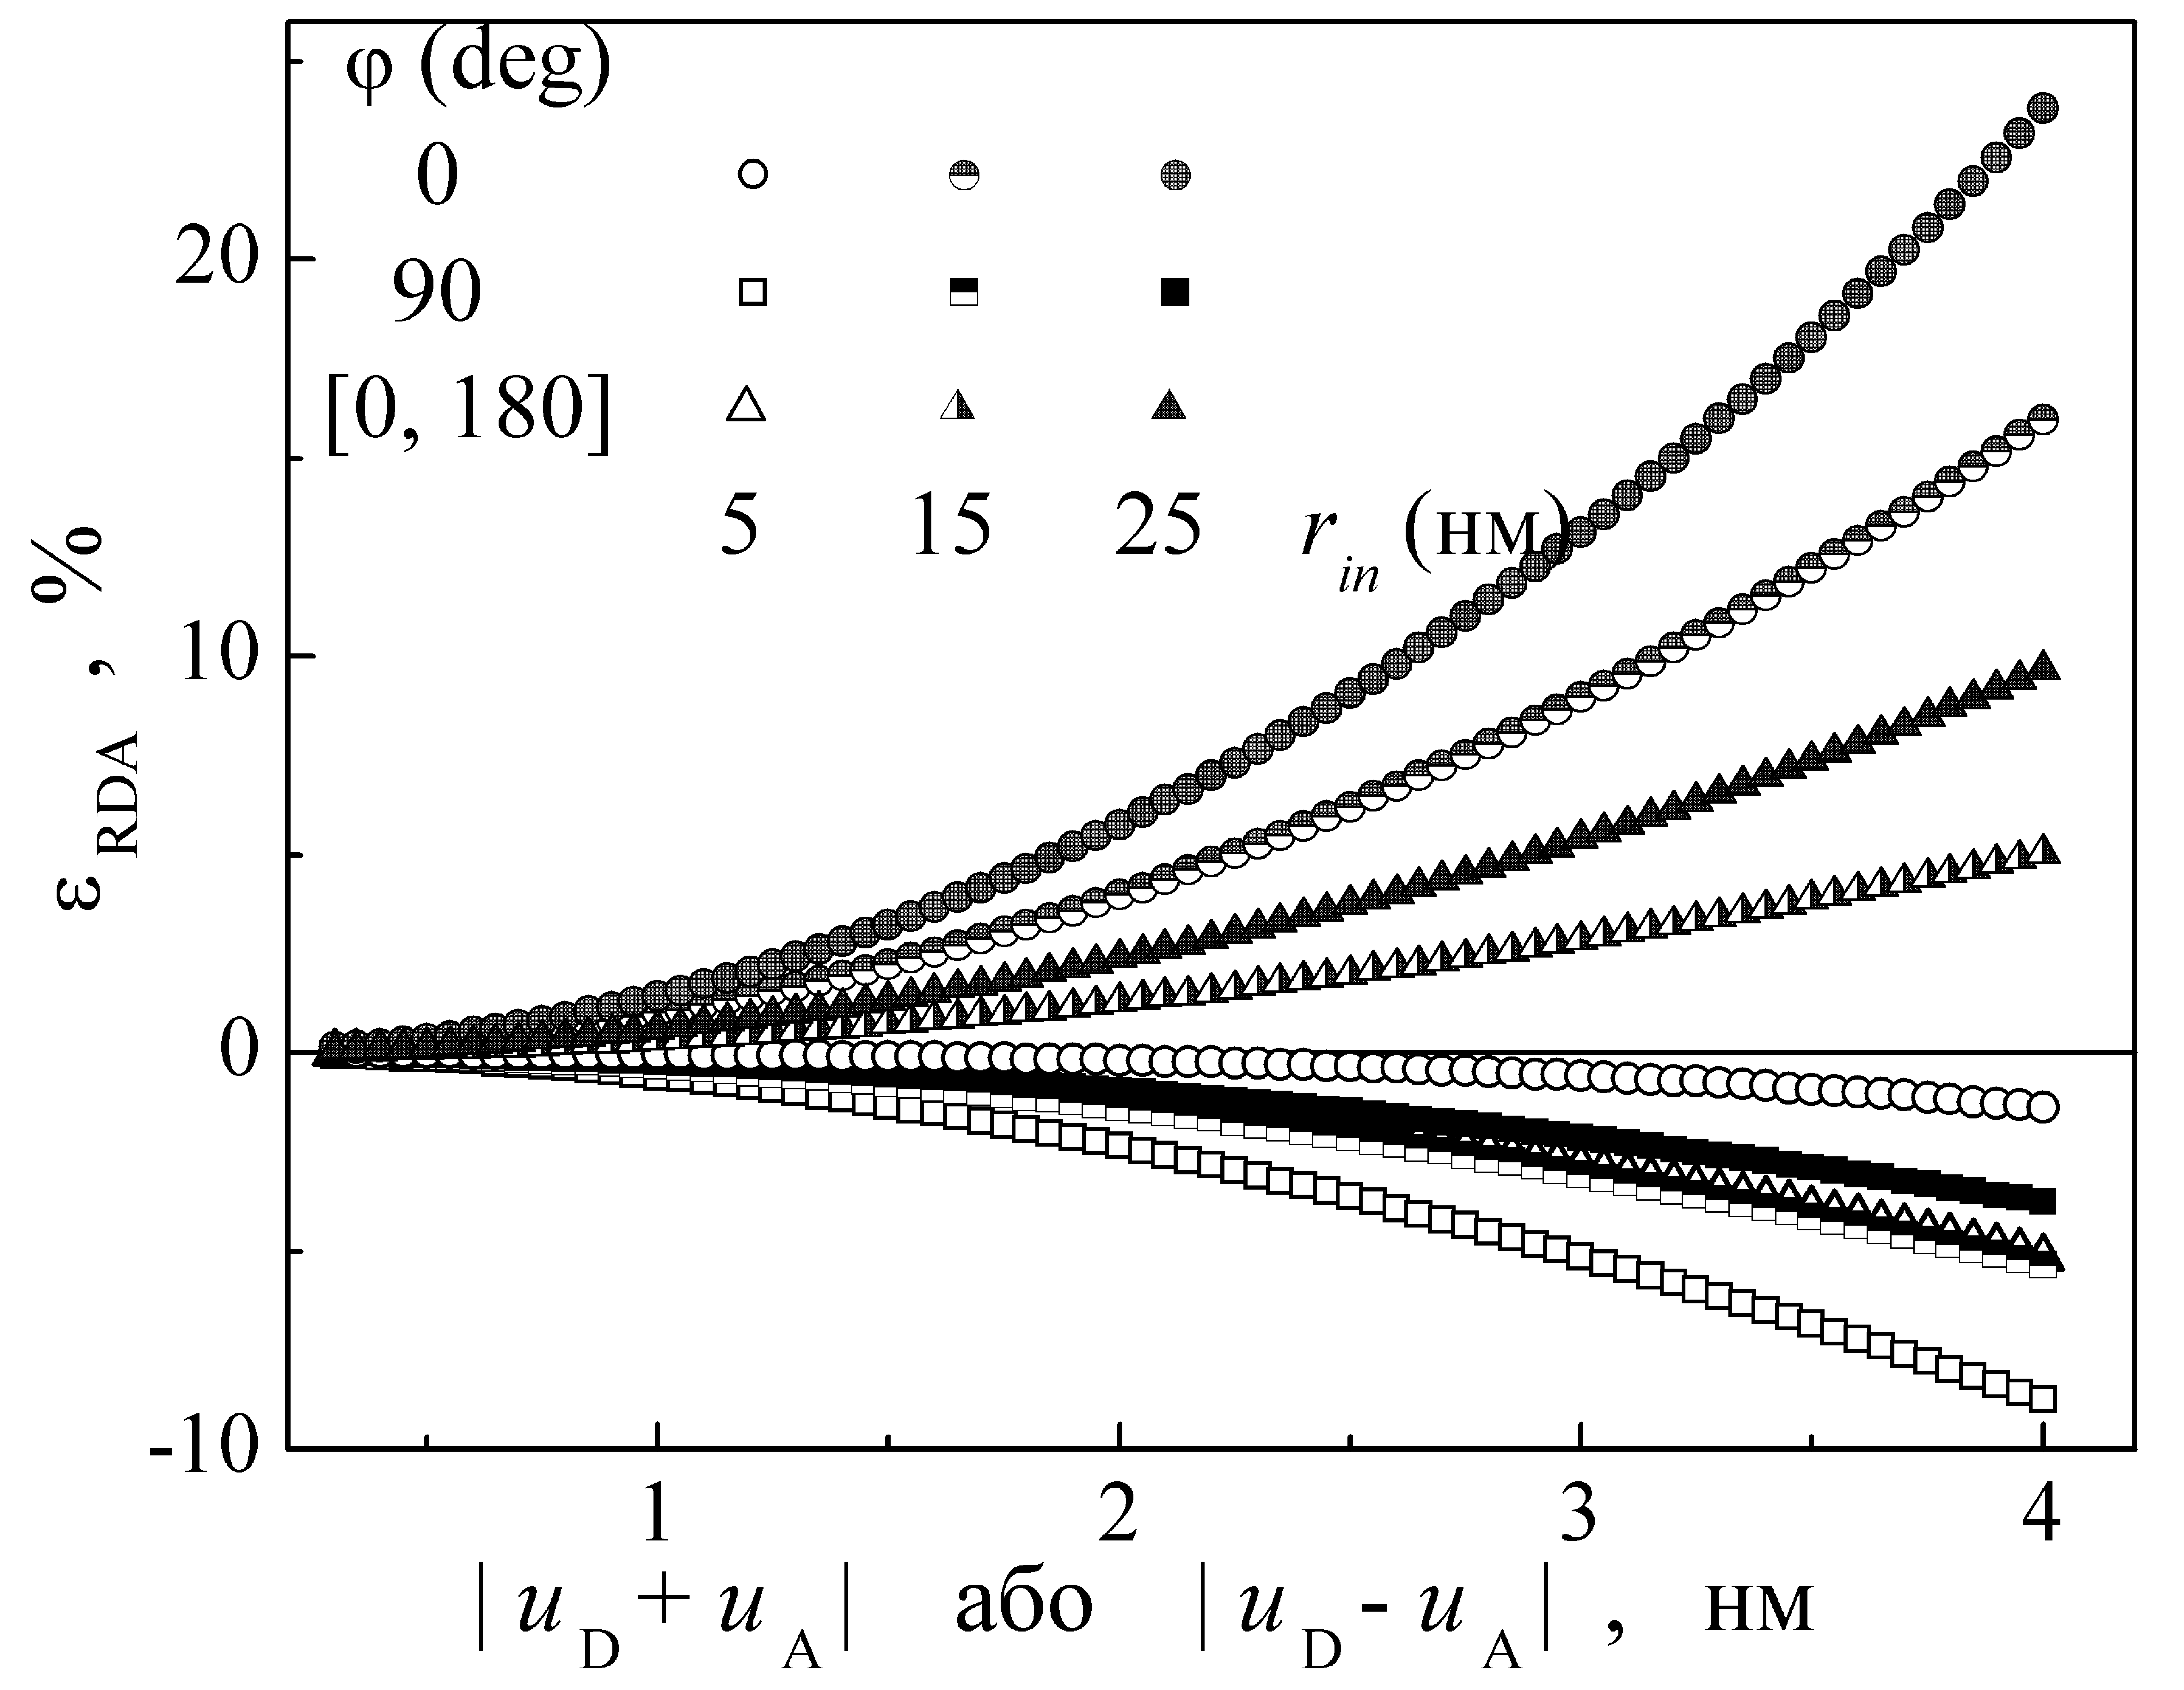
\includegraphics[width=0.75\textwidth]{fig_Erda}
\caption{\label{fig_Erda}
Розраховані залежності АІ змін параметру зв'язку від амплітуди коливань.
По горизонталі відкладено $|u_\mathtt{D}-u_\mathtt{A}|$ для випадків $\delta=0^\circ$ та
$|u_\mathtt{D}+u_\mathtt{A}|$ при $\delta=180^\circ$.
При розрахунках вважалося, що
$a_B=3.23$~нм,
$r_{in}=5$~нм (незаповнені точки), $15$~нм (напів--заповнені точки) та $25$~нм (заповнені точки),
$\varphi=0^\circ$ (кола), $90^\circ$ (квадрати).
Трикутники відповідають середнім значенням $\varepsilon_{\mathtt{RDA}}$,
обчисленим для діапазону $\varphi$ від $[0^\circ$ до $180^\circ]$.
}%
\end{figure}

Залежність відносної зміни ППЗ від амплітуди коливань має подібний характер, більше того
вона не залежить від $\varphi$:
\begin{equation}
\label{eqEpsSig}
\varepsilon_{\sigma}=\frac{(u_\mathtt{D}\pm u_\mathtt{A})^2}{2\,r_{in}^2}\,,
\end{equation}
де
знаки <<$+$>> та <<$-$>> відповідають випадкам $\delta=180^\circ$ та $\delta=0^\circ$, відповідно.
Тобто, при $(\Delta\Omega_d^\mathtt{D}\cdot\Delta\Omega_d^\mathtt{A}<0)$ ефективність впливу УЗ має бути більшою,
так як в цьому випадку вона визначається сумою зміщень компонент пари,
тоді як в протилежному --- їх різницею


Враховуючи, що $u_\mathtt{D},u_\mathtt{A}\sim \xi_\mathtt{US}\sim u_\mathtt{US}\sim \sqrt{W_\mathtt{US}}$,
остання формула може бути записана у вигляді
\begin{equation}
\label{eqEpsSigUS}
\varepsilon_{\sigma}=K_\mathtt{US}^\mathtt{DA}\,\,u_{\mathtt{US}}^2=K_\mathtt{US}^\mathtt{DA*}\,\,W_{\mathtt{US}}\,,
\end{equation}
де $K_\mathtt{US}^\mathtt{DA}$ ($K_\mathtt{US}^\mathtt{DA*}$) характеризує взаємодію УЗ з парою донор--акцептор
та залежить від властивостей дефектів та кристалічної ґратки (і ще й від типу хвиль для $K_\mathtt{US}^\mathtt{DA*}$).

Звичайно, можлива орієнтація пари зумовлена мінімізацією її повної енергії, а отже існують визначається кристалографічними осями.
Проте, з одного боку, врахуємо що кристали кремнію характеризуються кубічною симетрією і містять достатньо велику кількість еквівалентних напрямів.
З  іншого боку, необхідно врахувати,
що струм, пов'язаний з CDLR процесами протікає переважно в околі протяжних дефектів \cite{CDLR:JAP,CDLR:SSP}.
Нарешті, дислокації в ОПЗ нерідко розташовуються перпендикулярно площині $p-n$ переходу
і досліджені структури не є винятком (див. параграф~\ref{sbRsh}).
Якщо дефектна пара та дислокація розташовані поблизу один одного, то дислокація з крайовою компонентою буде впливати на просторове розташування пари.
Як наслідок, у ідеальному випадку пара донор--акцептор з  $(\Delta\Omega_d^\mathtt{D}\cdot\Delta\Omega_d^\mathtt{A}>0)$ переважно будуть орієнтовані
паралельно дислокаційній лінії,
тоді як вісь спарених дефектів з $(\Delta\Omega_d^\mathtt{D}\cdot\Delta\Omega_d^\mathtt{A}<0)$ має утворювати з дислокаційною лінією прямий кут.
При цьому, при поширенні УЗ перпендикулярно площині $p-n$ переходу (як в експериментах)
%використанні поперечних хвиль (зміщення паралельні площині $p-n$ переходу)
найбільш цікавими будуть наступні випадки

\noindent при  $\delta=0^\circ$ (випадок $\Delta\Omega_d^\mathtt{D}\cdot\Delta\Omega_d^\mathtt{A}>0$):
\begin{center}
\noindent   $\varphi=90^\circ$ (поперечні хвилі)  та $\varphi=0^\circ$ (повздовжні хвилі)
\end{center}

\noindent при  $\delta=180^\circ$ (випадок $\Delta\Omega_d^\mathtt{D}\cdot\Delta\Omega_d^\mathtt{A}<0$):
\begin{center}
\noindent   $\varphi\in[0^\circ\div 180^\circ]$ (поперечні хвилі)  та $\varphi=90^\circ$ (повздовжні хвилі).
\end{center}

Іншими словами,
якщо зміна об'єму кристалу, пов'язана з донором, протилежна за знаком зміні об'єму кристалу, пов'язаній з акцептором, то
при поширенні поперечних хвиль можуть реалізуватися випадки, які відповідають всім кривим на Рис.~\ref{fig_Erda}.
Якщо ж $\Delta\Omega_d^\mathtt{D}\cdot\Delta\Omega_d^\mathtt{A}>0$, то потрібно брати до уваги лише криві, для позначення
яких використано квадрати.


Таким чином, в рамках запропонованої моделі очікується, що УЗН спричинює зміну відстані між донором та акцептором,
що стає причиною появи $\varepsilon_{\sigma}$ та $\varepsilon_{\mathtt{RDA}}$, величина яких переважно визначається АІ зміщенням атомів.
Згідно з CDLR теорією,
збільшення ППЗ та зменшення параметру зв'язку має викликати зменшення часу життя носіїв та збільшення фактору неідеальності,
що і спостерігається на експерименті.


Запропонована модель може бути використана і для пояснень впливу УЗ на процеси рекомбінації в КНО (див. Рис.~\ref{figDUSTau}).
Так як АІ зміни оборотні, то зміна часу життя, згідно з (\ref{eqTAUSHRsum}), може бути пов'язана лише зі збільшенням
$\sigma_n$ в умовах УЗН.
Відомо, що переважна більшість рекомбінаційних центрів у кремнії є комплексними ТД,
причому компоненти комплексу не еквівалентні між собою.
Зокрема, нерідко вони характеризуються протилежним електричним зарядом.
В літературі \cite{CDLR:R2} запропоновано, що для подібних ТД також має виконуватись емпіричне співвідношення~(\ref{eqSigma}),
причому в такому випадку $r$ визначається відстанню між компонентами комплексного ТД, яка  менша, ніж відстань між донором та акцептором в CDLR.
В цьому випадку, згідно з описаною моделлю, УЗН також викликає зміну $r$ та $\sigma_n$ відповідно до виразу (\ref{eqEpsSigUS}).
Проте якщо для випадку CDLR зміна ППЗ носіїв донором (і/або акцептором) доповнюється зміною параметру зв'язку,
то при АІ варіація часу життя в КНО визначається лише модифікацією поперечного перерізу захоплення.

Ефективність АДВ залежить від типу дефекту та його структури \cite{UST:Medvid}
і не всі дефекти в кремнії є акусто активними (ААД).
Якщо $M_d^\mathtt{AA}$ та $M_d^\mathtt{nonAA}$ --- загальна кількість типів ААД та не акусто активних (non--AA) центрів,
то вираз (\ref{eqTAUSHRsum}) для $\tau_{n}^{-1}$ в умовах УЗН та без нього може бути записаний у вигляді
\begin{eqnarray}
\tau_{n,in}^{-1}&=&\sum_j^{M_d^\mathtt{AA}}N_{d,j}\,\sigma_{n,j}^{in}\,\upsilon_{\mathrm{th},n}+
\sum_l^{M_d^\mathtt{nonAA}}N_{d,l}\,\sigma_{n,l}\,\upsilon_{\mathrm{th},n}\,,\\
\tau_{n,\mathtt{US}}^{-1}&=&\sum_j^{M_d^\mathtt{AA}}N_{d,j}\,\sigma_{n,j}^\mathtt{US}\,\upsilon_{\mathrm{th},n}+
\sum_l^{M_d^\mathtt{nonAA}}N_{d,l}\,\sigma_{n,l}\,\upsilon_{\mathrm{th},n}\,.
\end{eqnarray}
Враховуючи, що $\sigma_{n,j}^\mathtt{US}=(\varepsilon_{\sigma,j}+1)\sigma_{n,j}^{in}$ останнє співвідношення може бути записано
у вигляді
\begin{eqnarray}
\label{eqEpsSigUSA}
\tau_{n,\mathtt{US}}^{-1}&=&\sum_j^{M_d^\mathtt{AA}}N_{d,j}\,\sigma_{n,j}^{in}\,\upsilon_{\mathrm{th},n}+
\sum_j^{M_d^\mathtt{AA}}N_{d,j}\,\sigma_{n,j}^{in}\,\varepsilon_{\sigma,j}\,\upsilon_{\mathrm{th},n}+
\sum_l^{M_d^\mathtt{nonAA}}N_{d,l}\,\sigma_{n,l}\,\upsilon_{\mathrm{th},n}=\nonumber\\
&=&\tau_{n,in}^{-1}+\sum_j^{M_d^\mathtt{AA}}N_{d,j}\,\sigma_{n,j}^{in}\,\varepsilon_{\sigma,j}\,\upsilon_{\mathrm{th},n}\,.
\end{eqnarray}
Взявши до уваги (\ref{eqEpsSigUS}), отримуємо
\begin{eqnarray}
\tau_{n,\mathtt{US}}^{-1}&=&\tau_{n,in}^{-1}+
\sum_j^{M_d^\mathtt{AA}}N_{d,j}\,\sigma_{n,j}^{in}\,K_\mathtt{US,j}\,\,u_{\mathtt{US}}^2\,\upsilon_{\mathrm{th},n}=\nonumber\\
&=&\tau_{n,in}^{-1}+u_{\mathtt{US}}^2\,\sum_j^{M_d^\mathtt{AA}}N_{d,j}\,\sigma_{n,j}^{in}\,K_\mathtt{US,j}\,\upsilon_{\mathrm{th},n}\,,
\end{eqnarray}
де $K_\mathtt{US,j}$ описує взаємодію УЗ з дефектом $j$--го типу.
Порівнявши з (\ref{eqMS_Us}) можемо сказати, що параметр $K_\mathtt{US}$, який кількісно описує експериментально виявлений вплив УЗ на час життя неосновних носіїв в базі КСЕ,
залежить від кількості АА дефектів та їх концентрації:
\begin{equation}
\label{eqKUS}
K_\mathtt{US}=\sum_j^{M_d^\mathtt{AA}}N_{d,j}\,\sigma_{n,j}^{in}\,K_\mathtt{US,j}\,\upsilon_{\mathrm{th},n}=\sum_j^{M_d^\mathtt{AA}}\frac{K_\mathtt{US,j}}{\tau_{n,j}^{in}}\,.
\end{equation}
Більше значення $K_\mathtt{US}$, отримане для SC17 (див. Таблицю~\ref{tabSSCParam}), свідчить про наявність у цьому зразку більшої кількості ААД та/або більшої їх концентрації.

Виявлена лінійність залежності зворотного часу життя від амплітуди атомних зміщень (див. Рис.~\ref{figKus},б) підтверджує
справедливість запропонованої моделі.
Крім того, зауважимо що так як початкова відстані $r_{in}$ між компонентами комплексного ТД, яка  менша, ніж початкова відстань між донором та акцептором в CDLR,
то, згідно з формулою~(\ref{eqEpsSig}), очікується що УЗ має більш ефективно впливати в першому випадку.
Саме таке співвідношення ($\varepsilon_{\tau n}>\varepsilon_{\tau g}$) і спостерігається на експерименті --- див. Таблицю~\ref{tabAIEfect}.


\subsection{Чисельний розрахунок залежностей напруги холостого ходу та фактора форми\label{sbVocSim}}

Як вже згадувалося раніше,
аналітичні вирази, які б відображали залежність напруги холостого ходу та фактора форми сонячного елементу
від $\tau_g$, $\tau_n$, $n_{\mathrm{id}}$ та $R_{sh}$ в рамках  моделі подвійного діода відсутні.
З метою візуалізації подібних залежностей були проведені чисельні розрахунки.
Вони полягали в тому, то використовуючи
формули (\ref{eqSSCIV})--(\ref{eqAlpha}) був синтезований набір ВАХ, які відповідали різним
значенням параметрів.
При цьому використовувалися значення параметрів, що були близькі до тих, якими характеризувалися досліджені КСЕ.
Після цього з штучних ВАХ використовуючи традиційний спосіб були визначені $V_{oc}$ та $F\!F$.
Типові приклади результатів обчислень, які відповідають температурі 320~K, наведено на Рис.~\ref{figVoc} та Рис.~\ref{figFF}.


\begin{figure}
\center
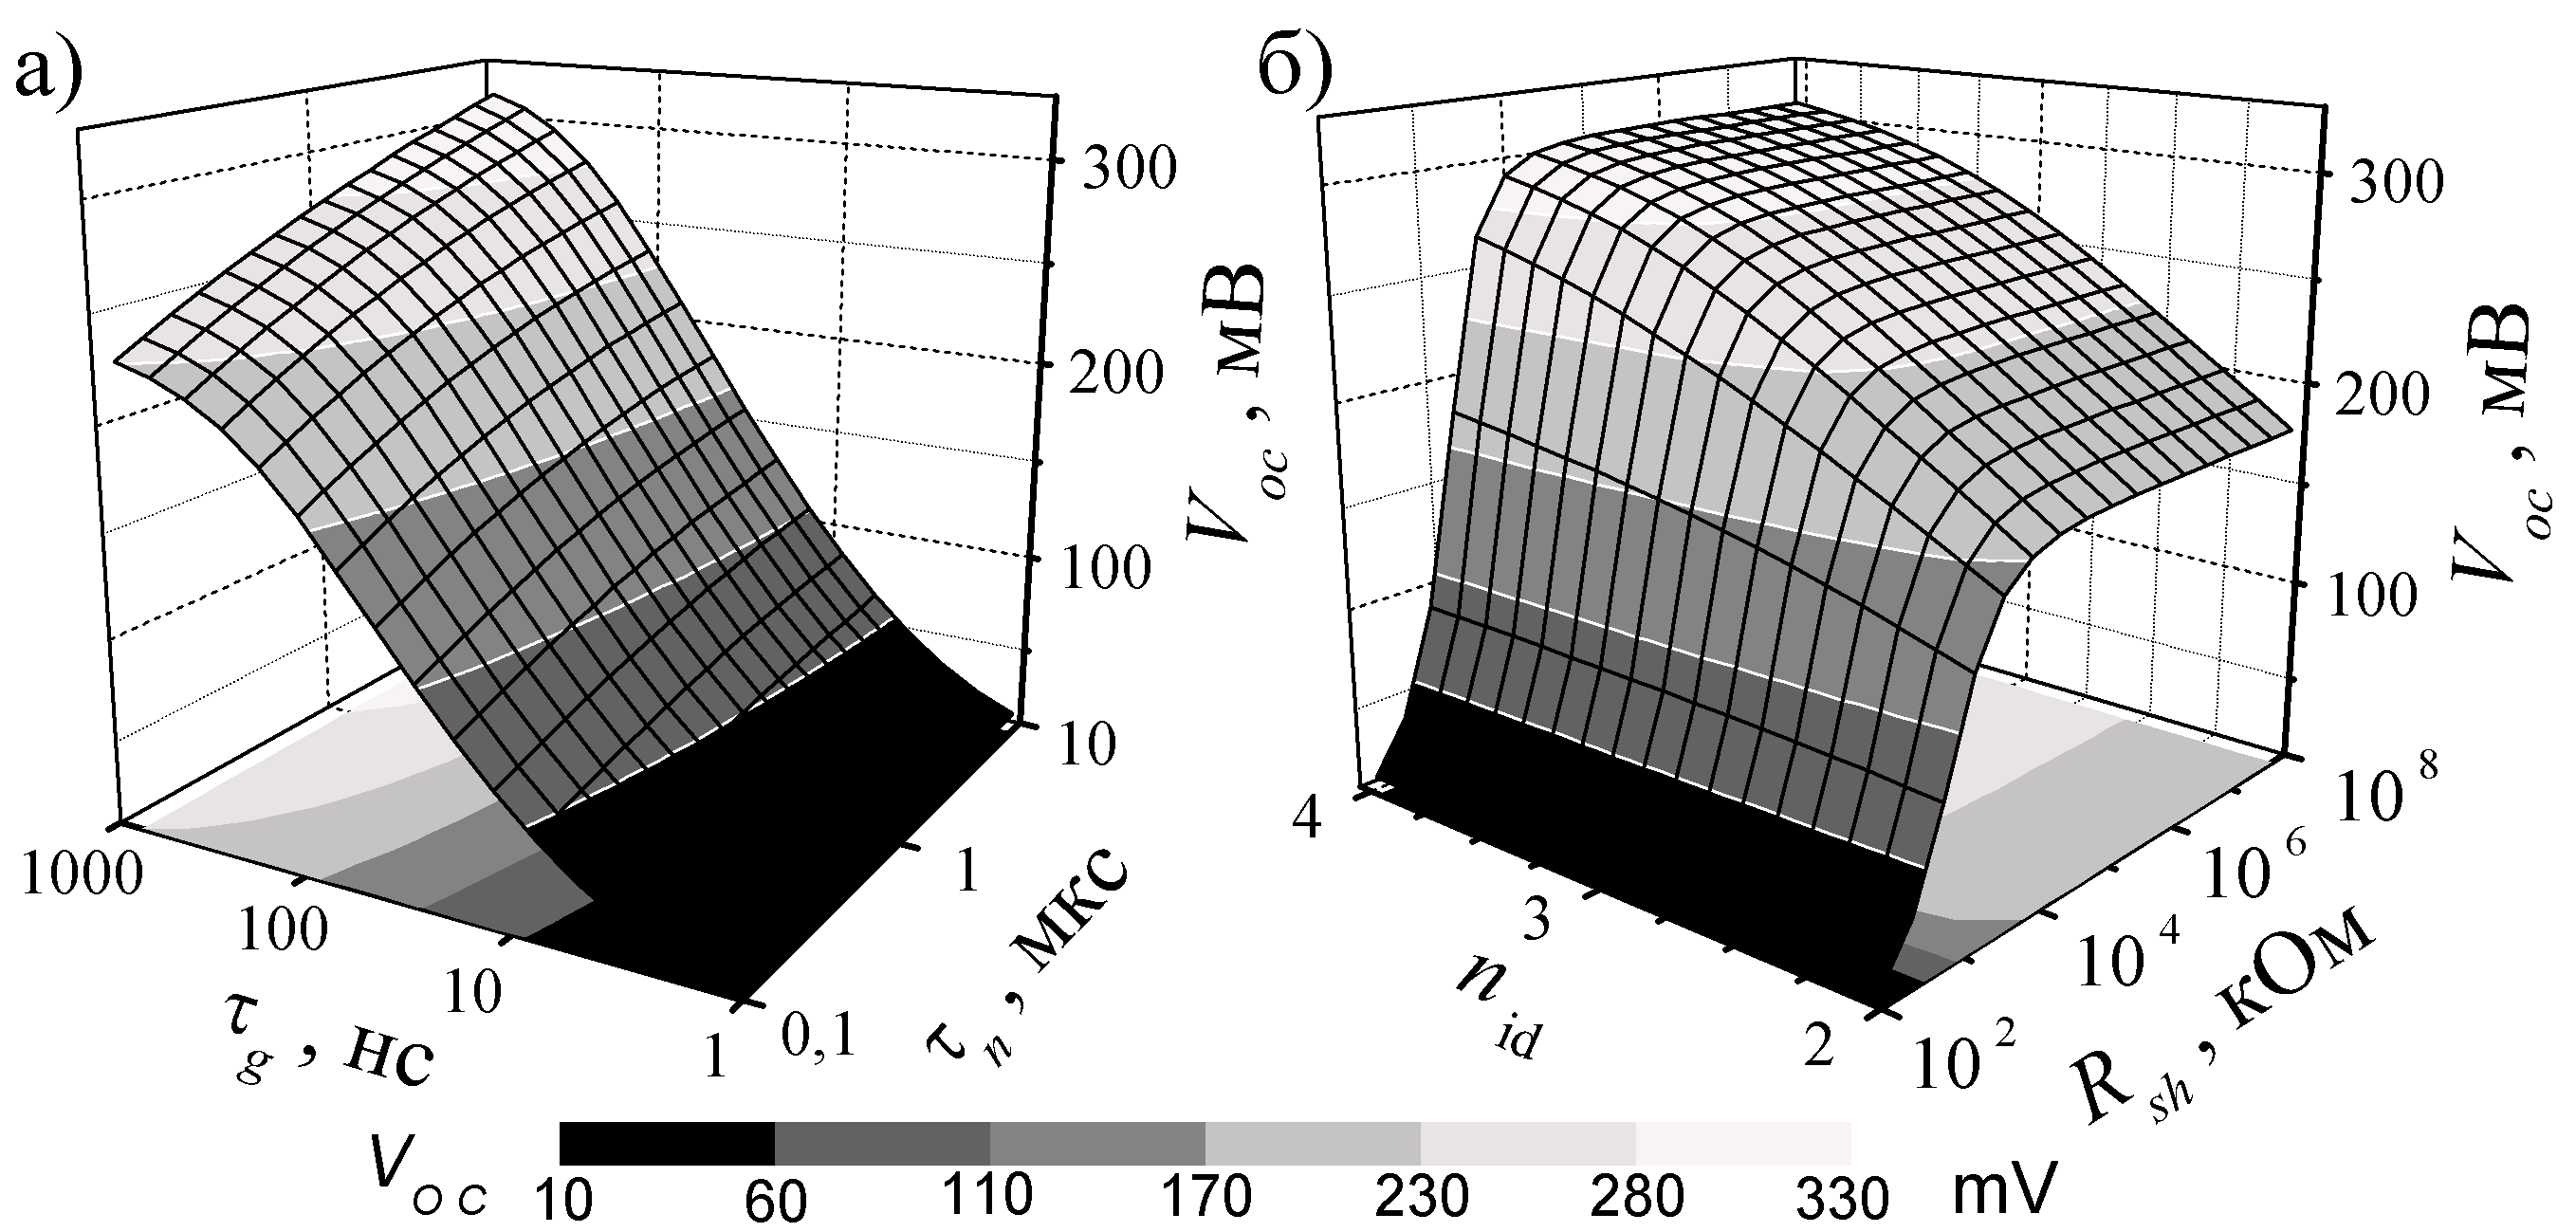
\includegraphics[width=0.95\textwidth]{figVoc}
\caption{\label{figVoc}
Результати моделювання в рамках моделі подвійного діоду залежності напруги холостого ходу КСЕ від часу життя носіїв заряду в ОПЗ та КНО (а) і
фактору неідеальності та шунтуючого опору (б).
При розрахунках вважалося, що $n_\mathrm{id}=2.55$ (a), $R_{sh}=5\times10^3$~Ом (a), $\tau_n=3\times10^{-6}$~с (б), $\tau_g=5\times10^{-8}$~с (б), $T=320$~K,
освітлення монохроматичне ($\lambda=900$~нм) та низькоінтенсивне ($W_{ph}=8$~Вт/м$^2$).
}%
\end{figure}


\begin{figure}
\center
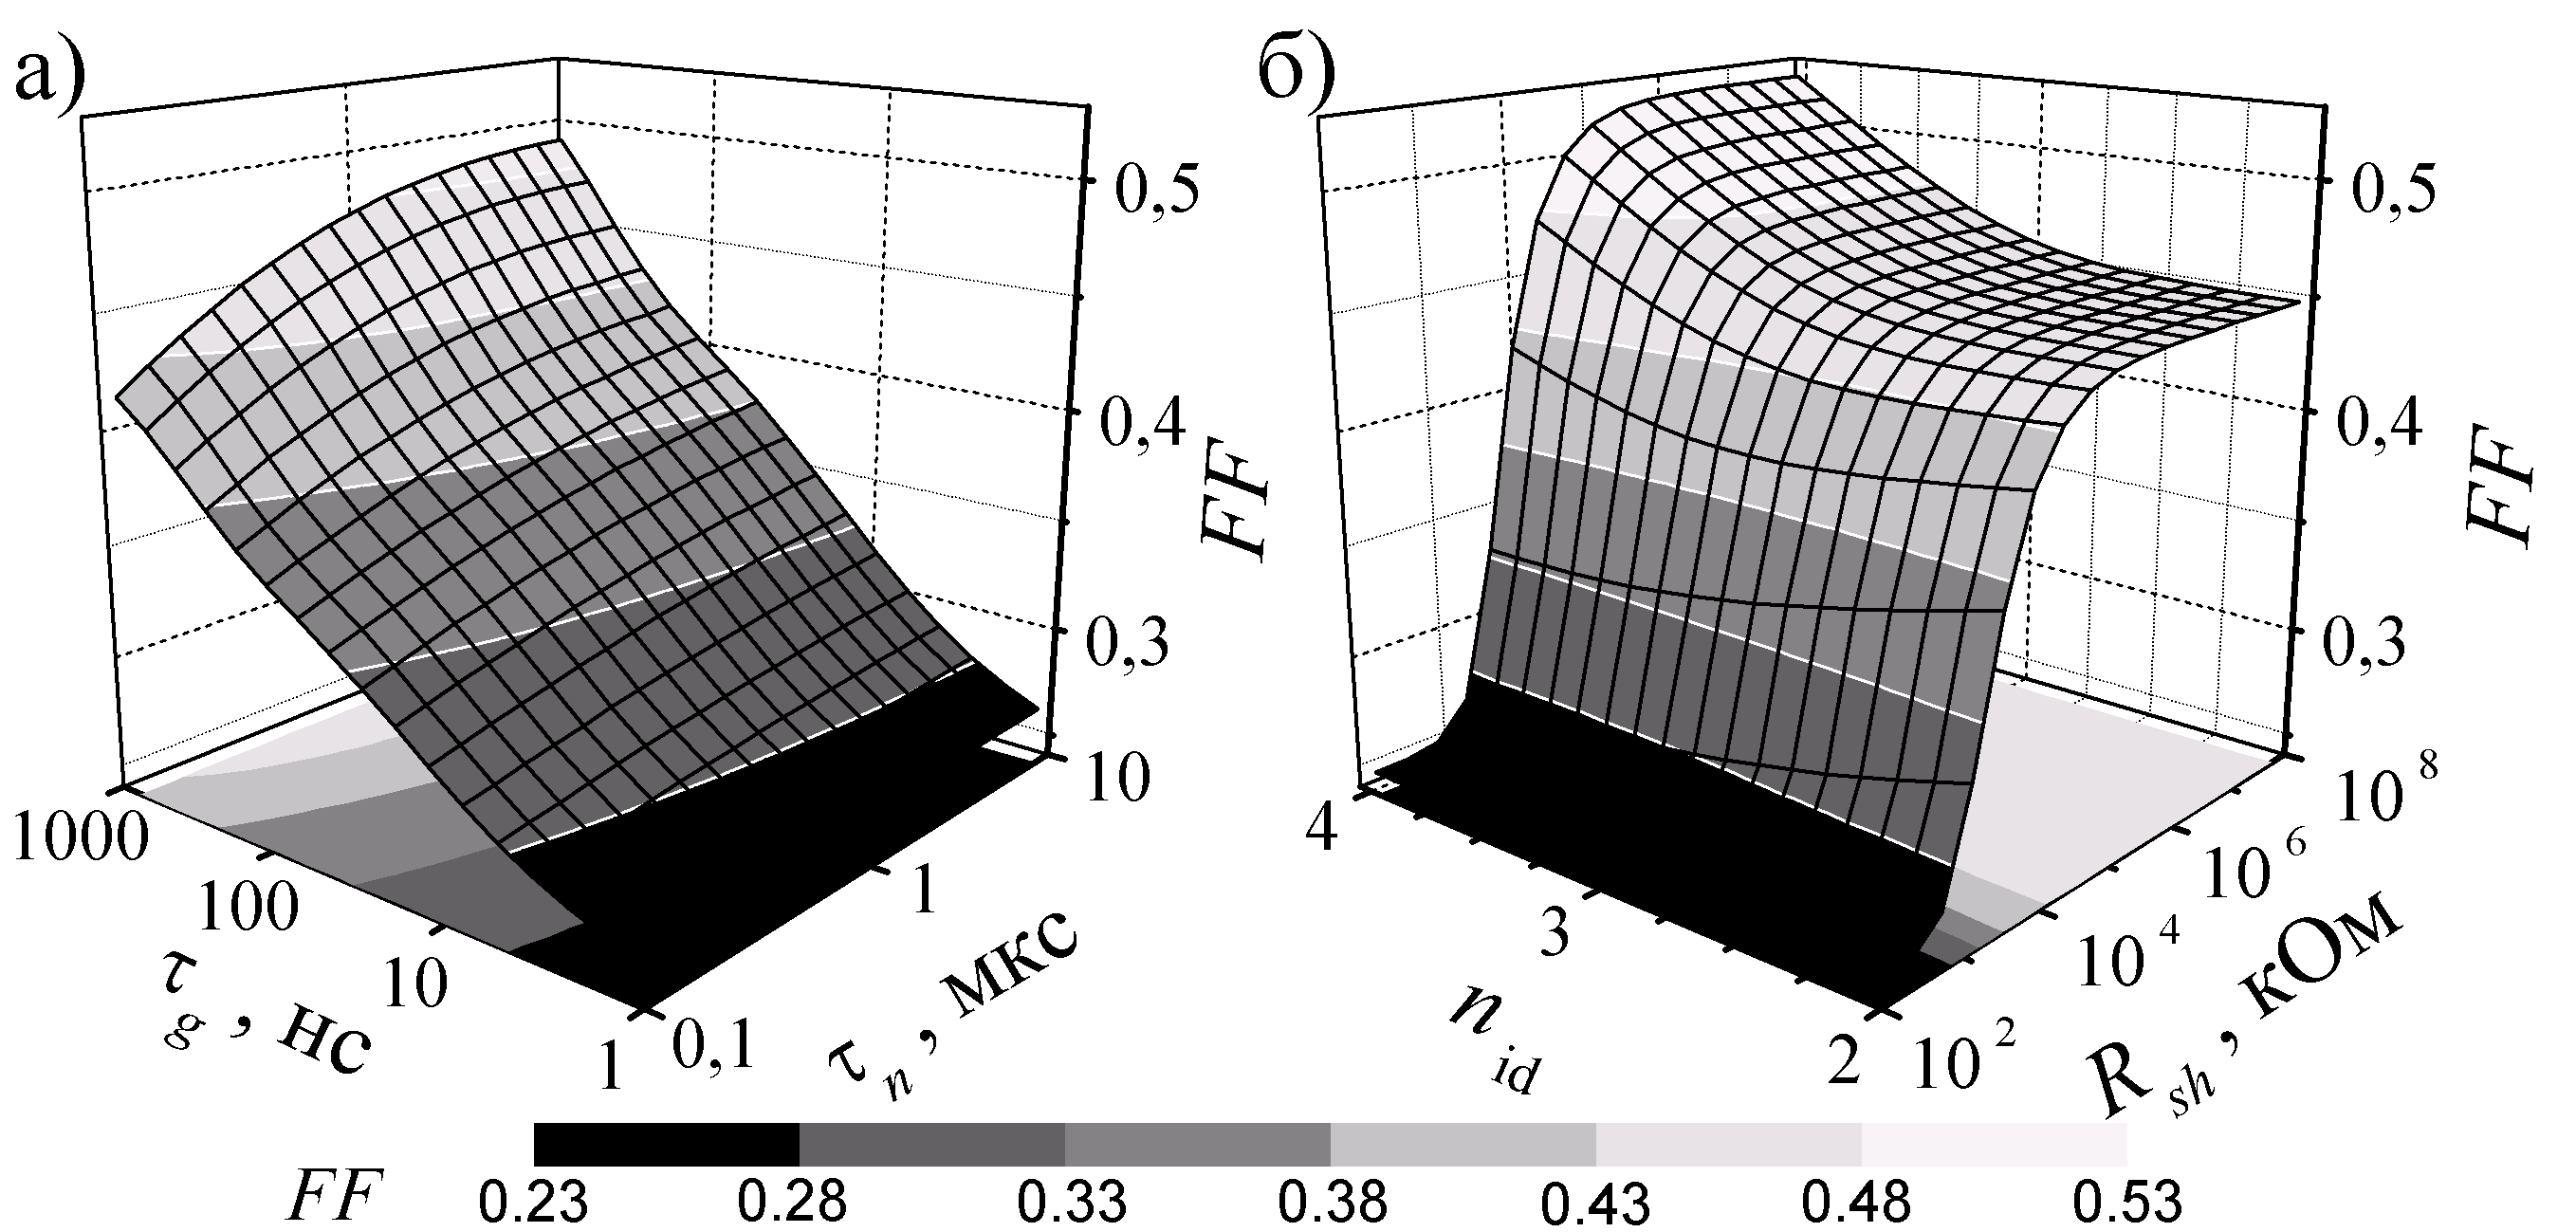
\includegraphics[width=0.95\textwidth]{figFF}
\caption{\label{figFF}
Результати моделювання в рамках моделі подвійного діоду залежності фактору форми СЕ від часу життя носіїв заряду в ОПЗ та КНО (а) і
фактору неідеальності та шунтуючого опору (б).
При розрахунках вважалося, що $n_\mathrm{id}=2.55$ (a), $R_{sh}=5\times10^3$~Ом (a), $\tau_n=3\times10^{-6}$~с (б), $\tau_g=5\times10^{-8}$~с (б), $T=320$~K,
освітлення монохроматичне ($\lambda=900$~нм) та низькоінтенсивне ($W_{ph}=8$~Вт/м$^2$).
}%
\end{figure}

Як видно з Рис.~\ref{figVoc},а та Рис.~\ref{figFF},а, зменшення $\tau_g$ викликає зменшення як $V_{oc}$, так і $F\!F$.
Водночас, для досліджених КСЕ напруга холостого ходу та фактор форми слабко залежать від
часу життя неосновних носіїв в КНО.

В свою чергу, Рис.~\ref{figVoc},б та Рис.~\ref{figFF},б показують,
що на величину $V_{oc}$ та $F\!F$ загалом впливає як $n_\mathrm{id}$, так і $R_{sh}$,
проте ступінь цих залежностей суттєво визначається величиною шунтуючого опору.
Наприклад, при $R_{sh}>10^5$~Ом (що відповідає випадку зразка SC17),
а)~$V_{oc}$ зростає з підвищенням величини фактора неідеальності;
б)~$V_{oc}$ та $FF$ практично не залежать від значення $R_{sh}$.
В той же час, при $R_{sh}\leq10^4$~Ом (випадок зразка SCR11),
а)~напруга холостого ходу та фактор форми зменшуються зі зменшенням шунтуючого опору;
б)~лише $F\!F$ слабко залежить від $n_\mathrm{id}$.

Таким чином, розглянута у параграфі \ref{sbQNR} зменшення $\tau_g$ викликає АІ деградацію як напруги
холостого ходу, так і фактора форми.
Цей ефект деградації підсилюється в SC11 внаслідок АІ зменшення $R_{sh}$ та частково компенсується в SC15
через АІ збільшення $n_\mathrm{id}$, що і пояснює відмінність величин $\varepsilon_{Voc}$ та $\varepsilon_{FF}$ в Таблиці~\ref{tabAIEfect}.




\subsection{Вплив інтенсивного освітлення на параметри КСЕ\label{sbDefectType}}
Раніше не було висловлено ніяких припущень, щодо того, які саме дефекти впливають на час життя
носіїв заряду та беруть участь у АДВ.
Даний параграф присвячений розгляду саме цього питання.

Відомо, що основними дефектами, які суттєво зменшують час життя носіїв в кремнії, вирощеному
за методом Чохральського та легованому бором, є
\begin{enumerate}[label=\asbuk*),leftmargin=0em,itemindent=1.5em]
\item  комплекси, що містять бор та кисень (так звані BO дефекти) \cite{LIDRev,LIDRev2};
\item пари залізо--бор \cite{MurphyJAP2011,FeB:Vahanissi,FeB:Schmidt} (або інші залізовмісні пастки, виявлені в $n^+-p$ переходах \cite{TeimurazPSS,TeimurazJAP});
\item кисневмісні преципітати \cite{MurphySC2014,Oxide_Schon,MurphyJAP2011,MurphyJAP2012,Oxide:Chen,Oxide:Porrini}.
\end{enumerate}
Дефекти перших двох типів чутливі до інтенсивного освітлення при кімнатних температурах.
З метою виокремлення впливу окремих дефектів на процеси, що відбуваються у досліджених КСЕ,
після закінчення дослідження впливу УЗ на їх параметри
була застосована наступна експериментальна процедура.

Для інтенсивного освітлення зразків була використана галогенова лампа (інтенсивністю близько 2~Suns).
Освітлення проводилось при температурі близько 305~K,
час одного освітлення вар'ювався в інтервалі від 1 до 8~год.
Після освітлення зразки знаходилися в темряві при кімнатній температурі.
Протягом перших 5~год після закінчення освітлення проводилось вимірювання темнових ВАХ з інтервалом часу $10\div15$~хв.
Метод цих вимірів було визначення кінетики можливих оборотних змін параметрів КСЕ, викликаних освітленням.
Для оцінки величини необоротних змін, також було проведено вимірювання ВАХ та визначення параметрів через 48~год
після освітлення.
Після того, як сумарний час інтенсивного освітлення досягав величини порядку 15~год,
проводився відпал зразків у темряві при температурі 200~$^\circ$C тривалістю 10~хв,
після якого при кімнатній температурі знову проводилось визначення параметрів.
Після цього цикли освітлення--відпал повторювався.

Відомо \cite{LIDRev,LIDRev2}, що інтенсивне освітлення викликає перетворення BO дефектів, що, в свою
чергу, призводить до суттєвого (до 10~\% від вихідного значення при тривалому освітленні) зменшення часу життя неосновних носіїв.
При кімнатній температурі ці зміни є залишковими, ВО дефекти не повертаються до вихідної конфігурації.
Проте десяти--хвилинний відпал при 200~$^\circ$C відновлює рекомбінаційні параметри кристалу, причому
якщо відпал відбувався у темряві, то дефекти повертаються до початкової конфігурації і знову можуть деградувати під
дією світла \cite{BO:Halam2016,LIDRev2,Kim}.

Таким чином, якщо якийсь з параметрів ($\tau_g$, $\tau_n$, $n_{\mathrm{id}}$ чи $R_{sh}$) визначається ВО дефектами,
то внаслідок вибраної експериментальної процедури мають спостерігатися його необоротні зміни після інтенсивного освітлення і відновлення
величини після відпалу.
Якщо припустити, що в досліджених КСЕ конфігурація ВО дефектів одразу відповідала деградованому стану,
то описані в попередньому реченні перетворення мають спостерігатися після першого відпалу.

На Рис.~\ref{figLight} показані стаціонарні значення параметрів зразків після освітлень та відпалів.
Як видно з наведених даних, для різних зразків були використані різноманітні режими.
Проте в будь--якому випадку, освітлення не викликає змін ні $\tau_g$, ні $\tau_n$, ні $n_{\mathrm{id}}$ як до
відпалу так і після.
Отже, можна виключити вплив комплексів, які містять бор та кисень, на рекомбінаційні процеси
як в ОПЗ, так і в базі діоду.

\begin{figure}
\center
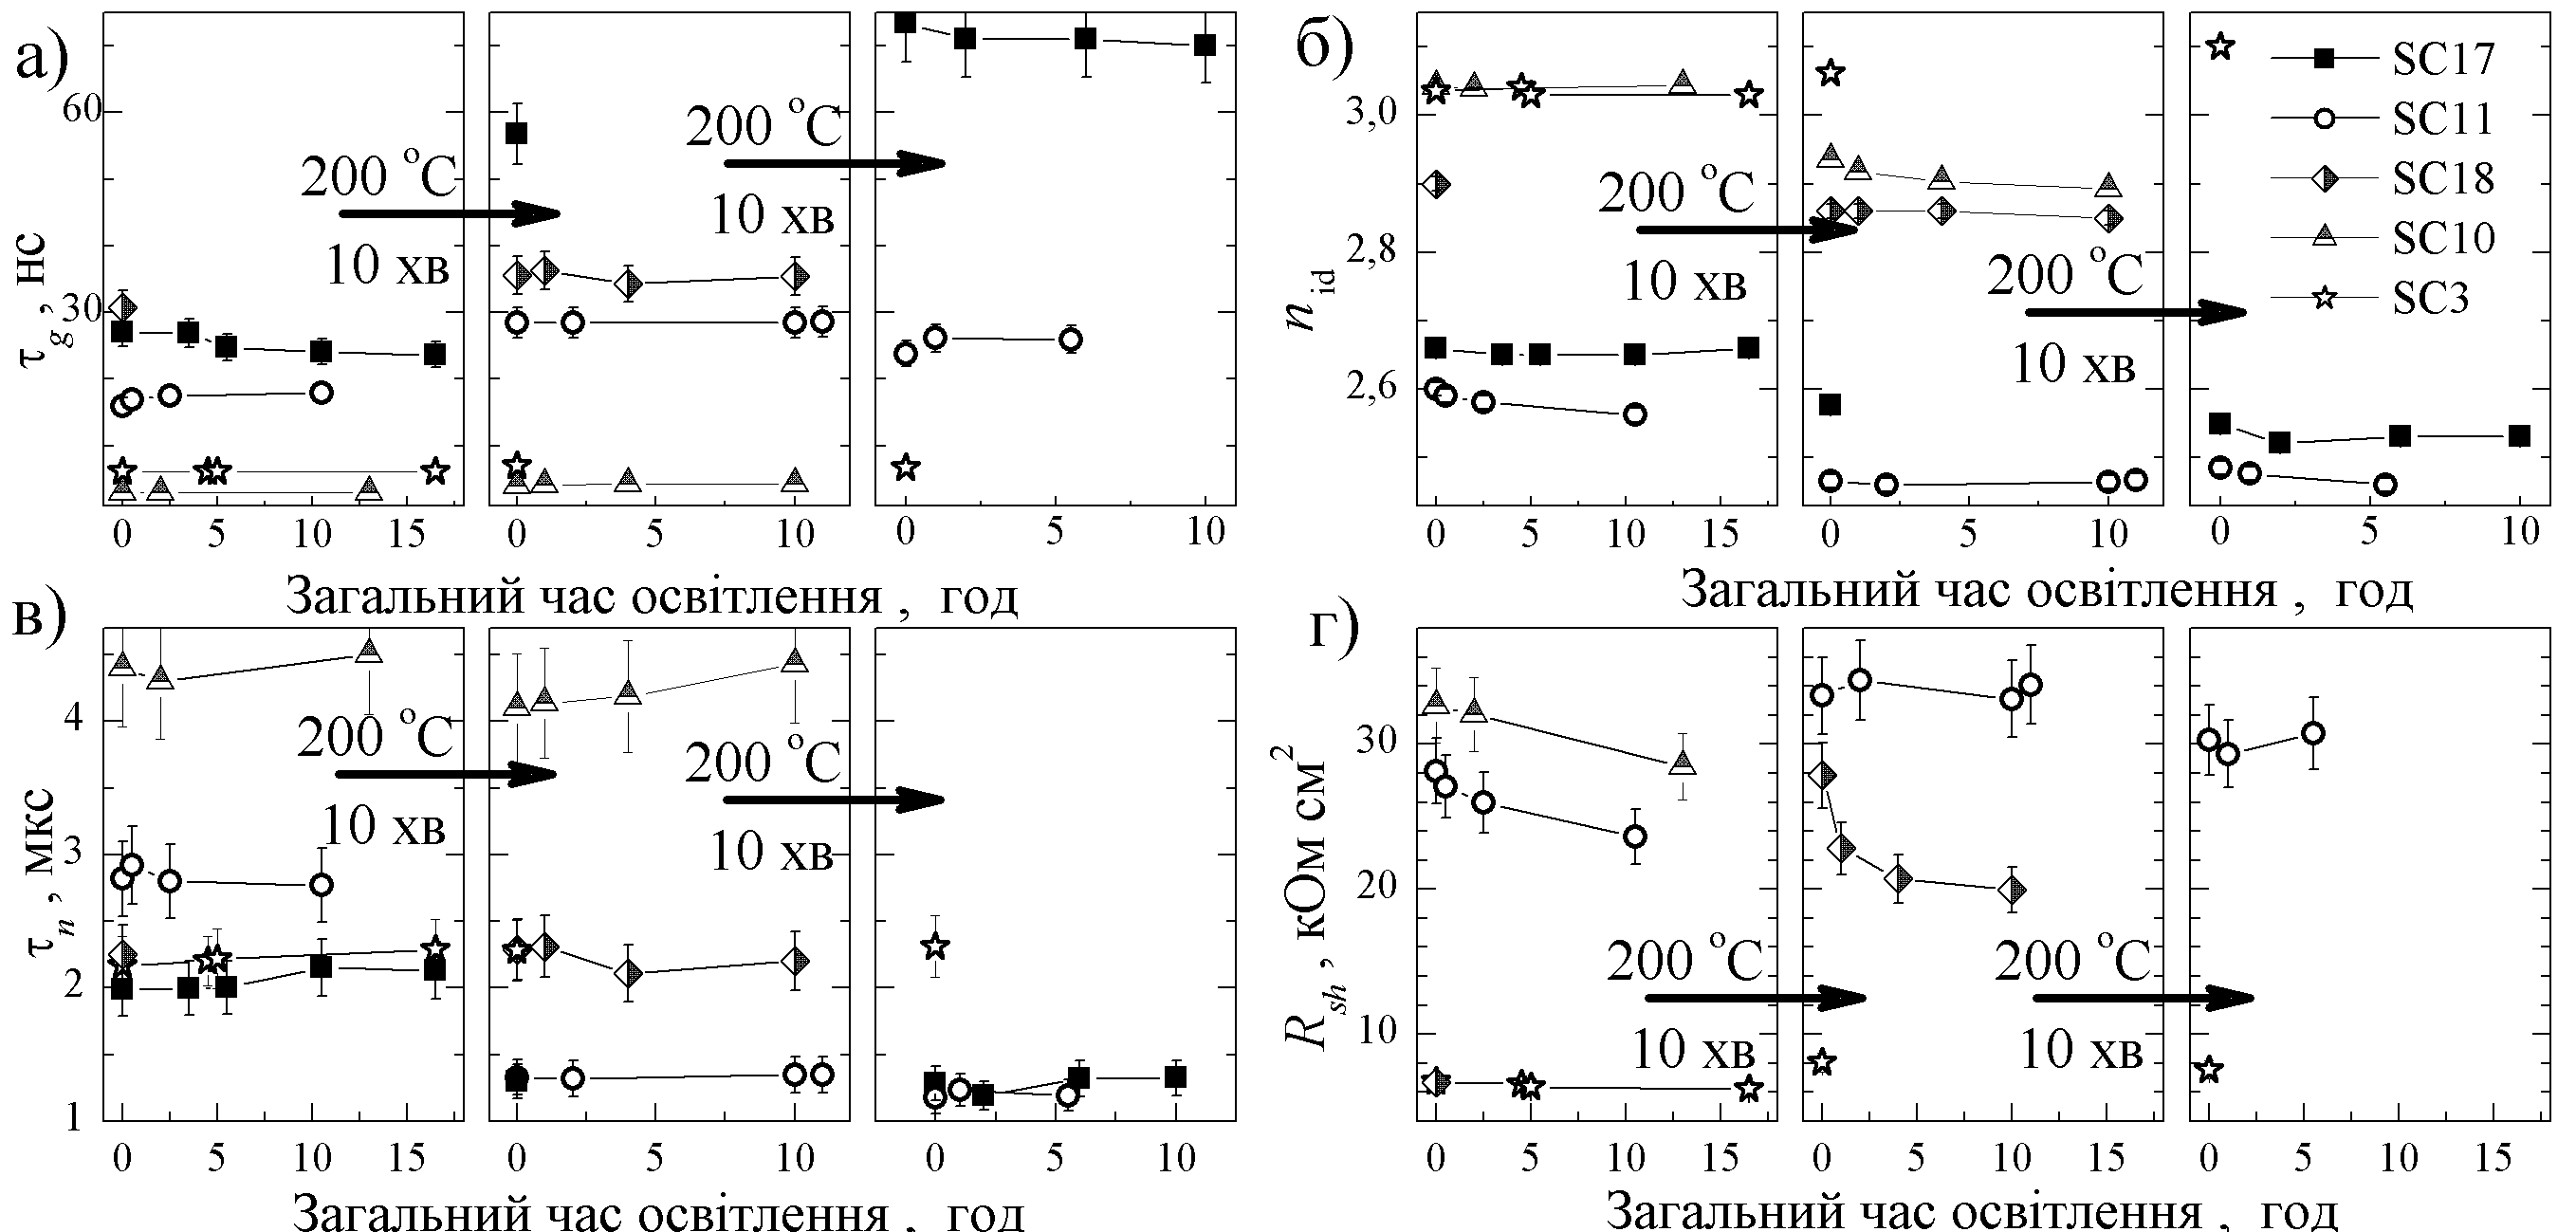
\includegraphics[width=1.0\textwidth]{figLight}
\caption{\label{figLight}
Залежності стаціонарних величин часу життя в ОПЗ (а),  фактору неідеальності (б), часу життя в КНО (в) та шунтуючого опору (г) від
повної тривалості високоінтенсивного освітлення та відпалу.
Лінії наведено лише для зручності.
Для зразка SC10 після першого відпалу значення $R_{sh}>10^{12}$~Ом$\cdot$см$^2$.
}%
\end{figure}


В Si:B переважна кількість домішкових атомів заліза утворює пари з бором.
Водночас пара Fe$_i$B$_s$ достатньо легко дисоціює і звільнені таким чином міжвузольні атоми заліза
викликають зменшення часу життя, яке залежить від рівня легування та концентрації надлишкових носіїв заряду \cite{FeB:Schmidt}.
Після припинення освітлення, в темряві, пари Fe$_i$B$_s$ відновлюються, при цьому
зменшення концентрації Fe$_i$ має описуватися виразом \cite{MurphyJAP2011,Wijaranakula}
\begin{equation}
\label{eqFeB}
N_{Fe}(t)=(N_{Fe,\,0}-N_{Fe,\,eq})\exp\left[-\frac{t}{\tau_{\mathtt{rep}}}\right]+N_{Fe,\,eq}\,,
\end{equation}
де
$N_{Fe,\,0}$ --- концентрація міжвузольних атомів безпосередньо після освітлення,
$N_{Fe,\,eq}$ --- рівноважна концентрація, яка досягається після тривалого перебування кристалу у темряві.
При цьому характерний час утворення пари $\tau_{\mathtt{rep}}$ залежить як від температури, так і від
рівня легування:
\begin{equation}
\label{eqTrep}
\tau_{\mathtt{rep}}=770\cdot p_p^{\,-2/3}\exp\left(\frac{E_{\mathtt{D,\,Fe}}}{kT}\right)\,,
\end{equation}
де
$E_{\mathtt{D,\,Fe}}=0,68$~еВ --- енергія активації дифузії Fe$_i$.


\begin{figure}
\center
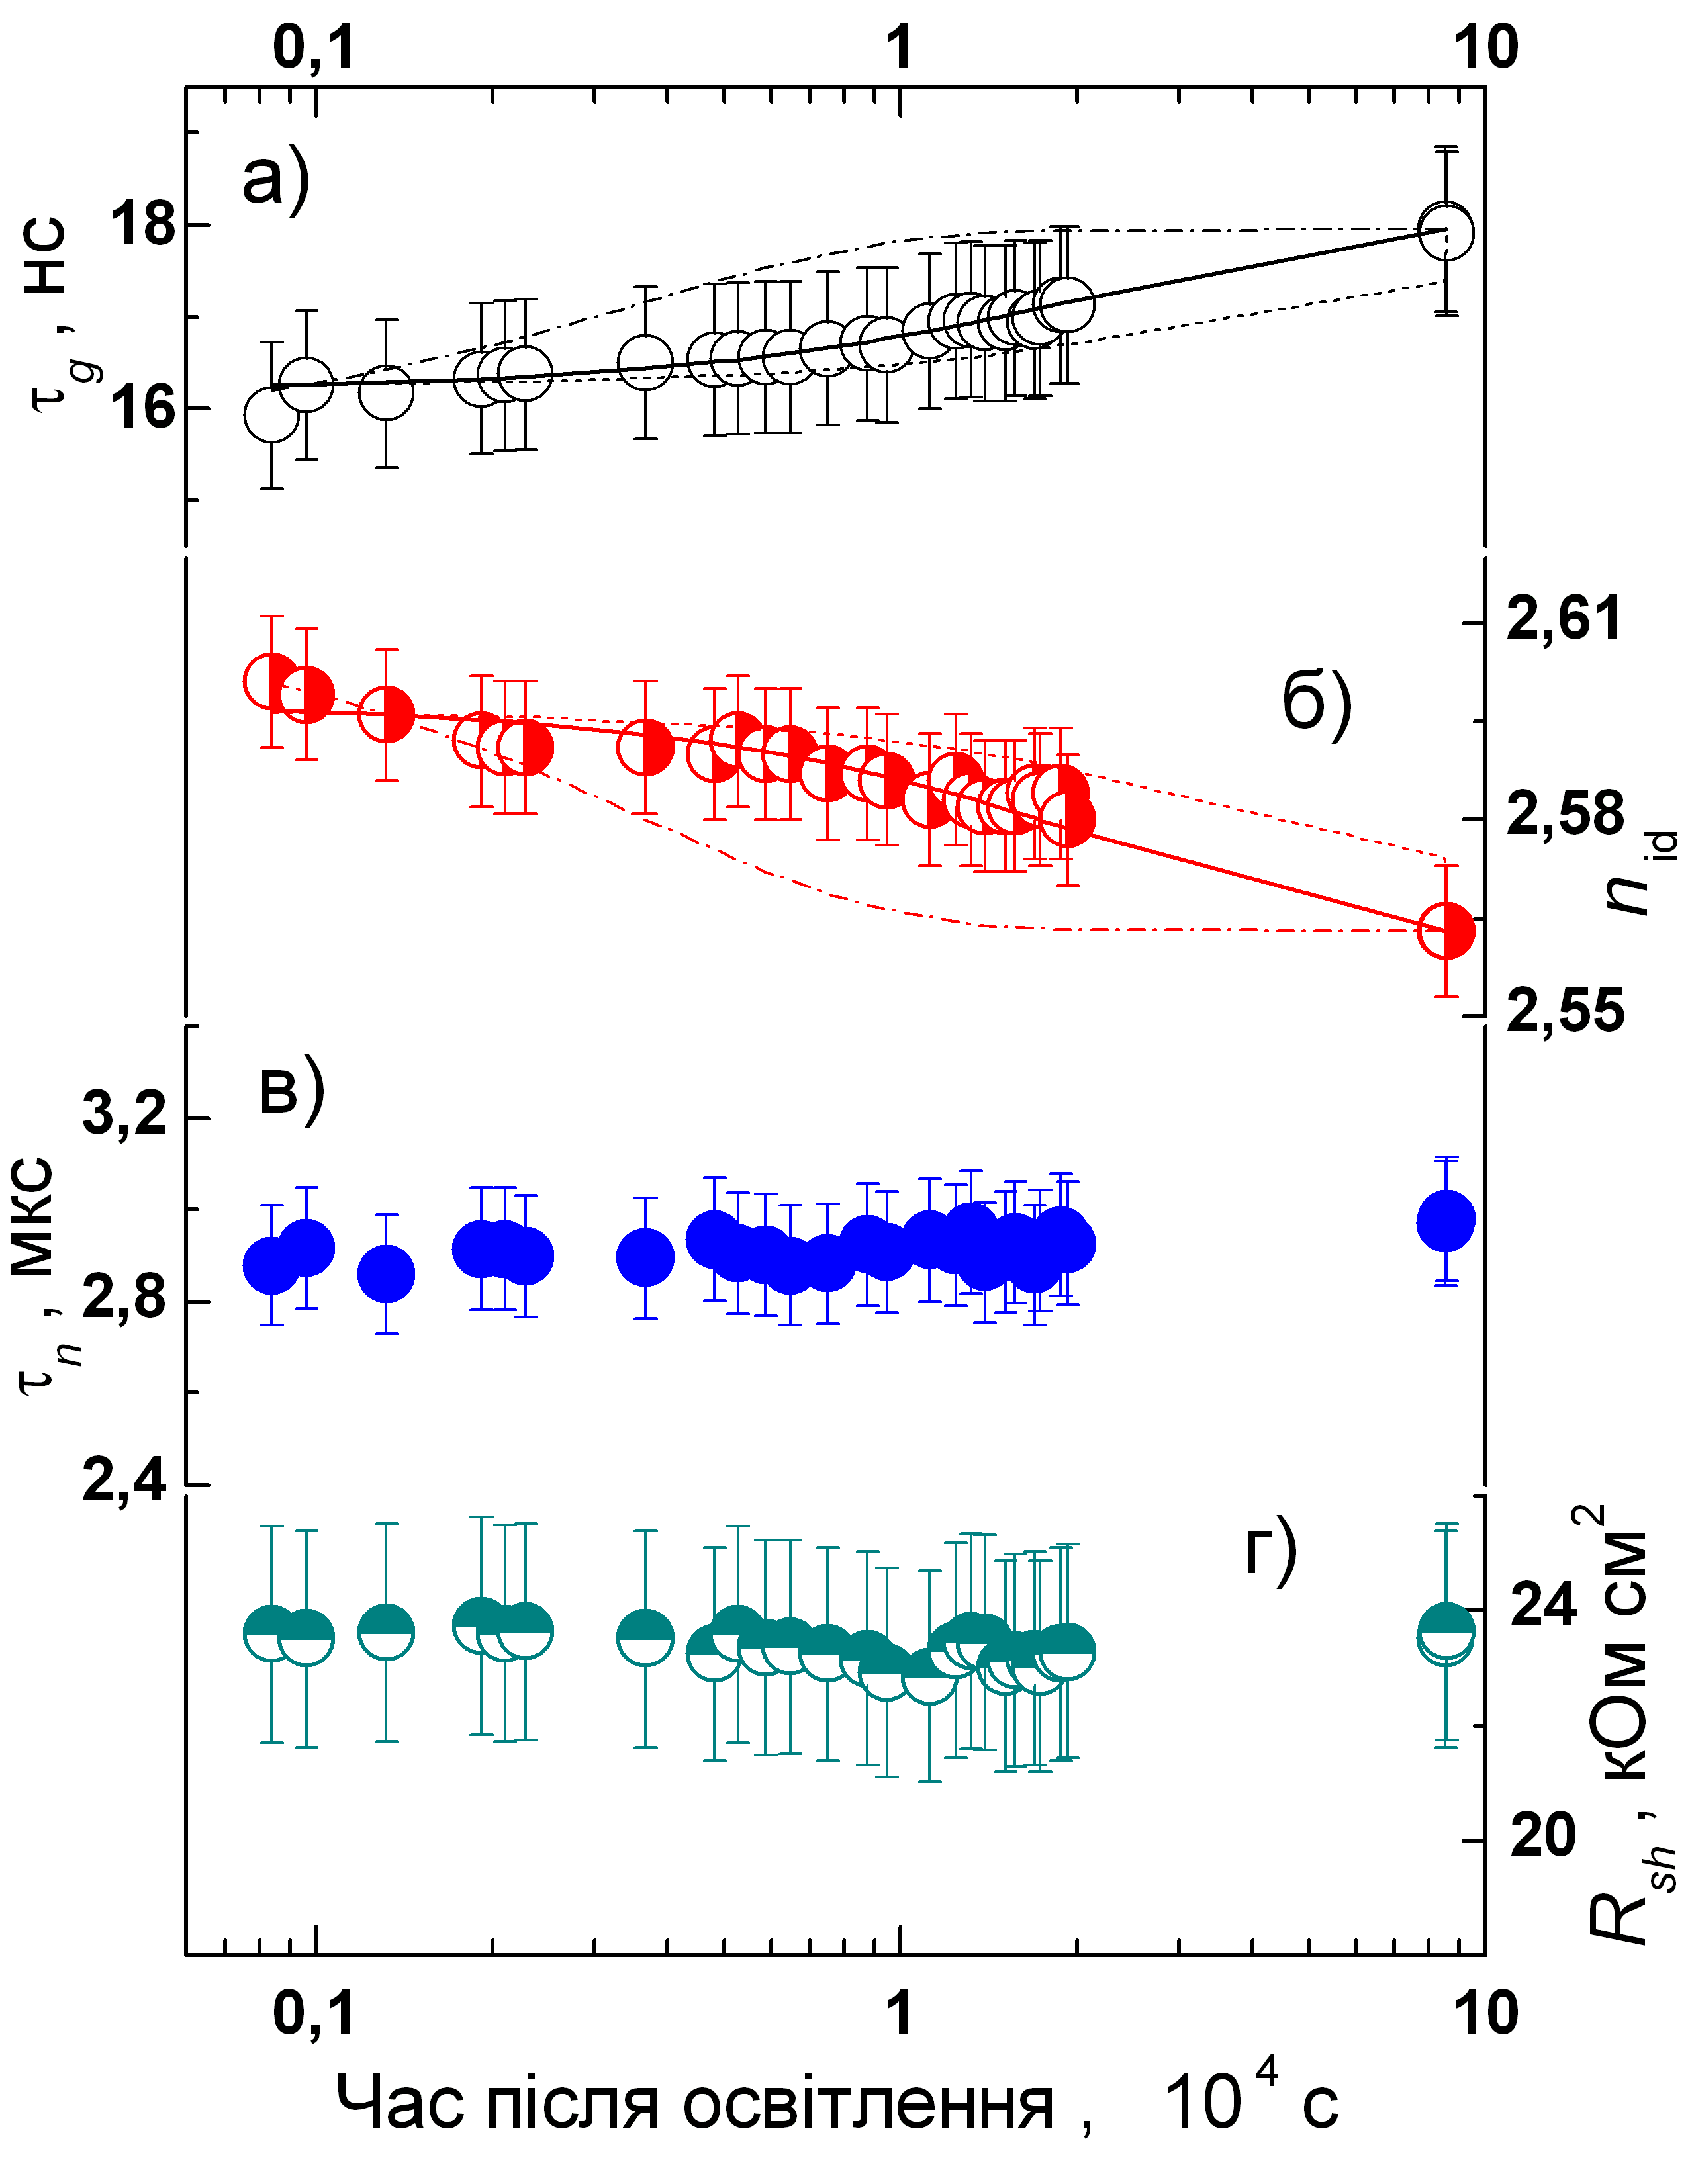
\includegraphics[width=0.65\textwidth]{figAfter}
\caption{\label{figAfter}
Залежність часу життя в ОПЗ (а),  фактору неідеальності (б), часу життя в КНО (в) та шунтуючого опору (г) від часу, що пройшов
після припинення освітлення.
Зразок SC11, $T=295$~K.
Точки --- результати вимірів,
лінії --- апроксимація з використанням формул (\ref{eqFeB}) та (\ref{eqTrep})
і $E_{\mathtt{D,Fe}}=0,63$~еВ (штрих--пунктирна лінія), 0,68~еВ (суцільна лінія) та 0,73~еВ (штрихова лінія).
}%
\end{figure}

Типова релаксаційна залежність зміни параметрів КСЕ після інтенсивного освітлення показана на Рис.~\ref{figAfter}.
Так як $\tau_n$ не змінюється після освітлення (див. Рис.~\ref{figAfter},в), то можна зробити висновок про те, що
пари Fe$_i$B$_s$ суттєво не впливають на час час життя в ОПЗ.

З іншого боку, виявлено збільшення $n_{\mathrm{id}}$ (приблизно на 0.03) та зменшення $\tau_g$ (приблизно на 10~\%) безпосередньо після освітлення
--- див. Рис.~\ref{figAfter},а та Рис.~\ref{figAfter},б.
В темряві ці зміни поступово зникають.
Було зроблено припущення, що еволюція $\tau_g$ та $n_{\mathrm{id}}$ може бути описана виразом, подібним до (\ref{eqFeB}).
При використанні величини $\tau_{\mathtt{rep}}=\left[1,3\cdot10^{-3}(1,4\times10^{15})^{\,2/3}\exp\left(-\frac{0,68}{295k}\right)\right]^{-1}=2,53\cdot10^4$~с,
яка очікується для відомого значення $E_{\mathtt{D,Fe}}=0,63$~еВ, апроксимуюча крива достатньо добре збігається з експериментальними даними
(суцільні лінії на Рис.~\ref{figAfter},a та б).
В той же час застосування іншої величина для $E_{\mathtt{D,Fe}}$ викликає суттєві відмінності між розрахованими та виміряними величинами
(штриховані лінії на цьому ж рисунку).
Отримані результати свідчать на користь того, що пара залізо--бор впливає
на рекомбінацію в ОПЗ.
Заряд пари в основному стані дорівнює <<+1>>, а отже у CDLR процесах має відігравати роль донора.
%, а її акцепторний рівень $E_c-0.26$~еВ \cite{MurphyJAP2011} приймає участь у CDLR процесах.
%При цьому
З одного боку, пара Fe$_i$B$_s$ є непоганим кандидатом на роль ААД:
бор є домішкою заміщення з іонним радіусом, який менший ніж для Si ($\Delta\Omega_d (\mbox{B}_s)<0$),
тоді як для міжвузольного заліза $\Delta\Omega_d (\mbox{Fe}_i)>0$.
Більше того,  в літературі \cite{Ostapenko1995,OlikhFTT} представлені результати впливу УЗН на цей дефект.
Проте з іншого боку, ППЗ електронів та дірок для Fe$_i$ та Fe$_i$B$_s$ відрізняються досить суттєво, в 1,7 та 0,04 рази, відповідно \cite{MurphyJAP2011}.
А так як, $\tau_g$ змінюється під дією світла незначним чином (приблизно на 10~\%, що навіть менше ніж в умовах УЗН), то це свідчить про
неосновну роль пари як у рекомбінаційних процесах в ОПЗ, так і в АДВ у цій області.


Таким чином, можна зробити висновок, що рекомбінація як в ОПЗ, так і в КНО відбувається, переважно,
завдяки кисневмісним преципітатам (КП).
За своєю будовою  це скупчення SiO$x$ ($1\leq x\leq2$), які утворюються всередині кристалу кремнію при підвищених температурах.
Розмір цих утворень коливається від декількох десятків до декількох сотень ангстрем залежно від режиму обробки.
При їх утворенні у загалом бездислокаційному Cz--Si виникають лінійні дефекти та дефекти пакування \cite{SiO:Hwang,SiO:Vanhell}.
Наявність КП суттєво впливає на час життя носіїв як в ОПЗ, так і в КНО.
наприклад, у кристалах з високою концентрацією преципітатів довжина дифузії неосновних носіїв може зменшуватись до декількох мікрон \cite{SiO:Hwang}.
Водночас КП виконують роль гетерів для домішкових атомів металів, які неминуче потрапляють у кристал під час виробництва
інтегральних схем і відіграють згубну роль для їх властивостей \cite{APR:Oxigen,MSER74}.
Цей процес гетерування є дуже важливим з точки зору збільшення відсотку виходу придатної мікроелектронної продукції.
Проте за наявності надмірної кількості КП та супроводжуючих їх появу дислокації
спостерігається зменшення механічної міцності Cz--Si \cite{MSER74}.


В досліджуваних зразках утворення певної кількості цих дефектів, і, відповідно, зменшення $\tau _n$ могло відбутися під час відпалу,
який застосовувався для переведення імплантованих іонів фосфору у електрично--активний стан.
Подібні процеси відомі з літератури.
Наприклад, в роботі \cite{SiO:Miyagi} показано, що відпал при температурі 750--850$^\circ$C
може викликати збільшення концентрації КП та зменшення часу життя.

З точки зору моделі CDLR це також цілком придатні об'єкти.
Дійсно, згідно з результатами, представленими в \cite{MurphySC2014,MurphyJAP2012},
рекомбінацію на SiO$x$ не можна пояснити використовуючи наближення одного дефекту, якому відповідає два рівні у забороненій зоні,
необхідно розглядати щонайменше два незалежних дефекти.
Цим дефектам відповідають рівні $E_v+0.22$~еВ та $E_c-0.08$~еВ, причому для них $\sigma_n/\sigma_p=157$ та $\sigma_p/\sigma_n=1200$ \cite{MurphyJAP2012}.
Тобто, ці дефекти цілком можуть виконувати роль донора та акцептора в моделі CDLR.
Як вже згадувалось, очікується, що процеси CDLR відбуваються переважно в околі лінійних дефектів \cite{CDLR:JAP,CDLR:SSP}.
Водночас, в літературі \cite{MurphySC2014,MurphyJAP2011,MurphyJAP2012} показано, що дислокації та дефекти пакування,
які оточують КП, можуть змінювати ППЗ та збільшувати концентрації двох вищеназваних дефектів,
проте не викликають появу  нових рівнів у забороненій зоні.

В літературі \cite{MurphyJAP2011} також показано, що ефективний коефіцієнт захоплення носіїв кисневмісними
преципітатами збільшується в декілька разів за умов перебування дефекту в полі механічних напруг.
В нашому випадку додатковим джерелом подібних напруг, поряд
з оточуючими КП дислокаціями та дефектами пакування, є УЗ і тому зменшення
часу життя носіїв може бути викликано і цією причиною також.

Скупчення SiO$x$, як правило, нерівномірно розподілені по площі пластини  Cz--Si \cite{Oxide_Schon} або сонячних елементів \cite{Oxide:Chen}.
Це може бути причиною зміни параметрів від зразка до зразка.
Нарешті,  стан КП залежить від обробки кристалу при підвищеній температурі.
В досліджених структурах відпал, на відміну від освітлення, викликає певні зміни параметрів (див. Рис.\ref{figLight}).
Виявлені зростання $\tau_g$ і $R_{sh}$ та спад $\tau_n$ і $n_\mathrm{id}$, на нашу думку, пов'язані саме з видозміною КП.

З іншого боку, дефекти різного типу зустрічаються в кремнієвих структурах одночасно.
Наприклад, у роботі \cite{BO:Fe} показано, що значна частина експериментальних особливостей зміни часу життя
внаслідок утворення ВО--дефектів може бути пояснена наявністю (та світло--індукованим розпадом) пар  Fe$_i$B$_s$.
А саме, визначальними для величини $\tau_n$ є комплекси, що містять бор та кисень, проте
наявність домішкового заліза впливає на процеси визначення параметрів кристалу.
Подібна супутникова роль пар Fe$_i$B$_s$ спостерігається і в нашому випадку.

Таким чином, на підставі зазначених вище даних, можна зробити висновок,
що дефектами, які приймають участь як у рекомбінаційних процесах, так і у акусто--дефектній взаємодії є, переважно,
кисневмісні преципітати.
Крім того, певний внесок у ці процеси пов'язаний з парами Fe$_i$B$_s$.

\section{Зміна активності рекомбінаційних центрів у кремнієвих $p$--$n$ структурах за умов ультразвукового навантаження\label{sBulyrMethod}}

\subsection{Метод визначення енергетичного положення рівнів в ОПЗ}

Методи нерівноважної модифікації дефектно--домішкової підсистеми з метою отримання нових властивостей напівпровідникових
кристалів, структур чи приладів, тобто методи так званої <<інженерії дефектів>> викликають все більшу зацікавленість дослідників \cite{Smirnov}.
Це зумовлено перспективами  створення за допомогою подібних методів елементної бази твердотільної
електроніки нового покоління за рахунок контрольованого формування та видозміни активних центрів або нанокластерів.
Безумовні, лідерами цієї галузі є радіаційні методи --- див., наприклад, \cite{Kozlovs,DefImplan}.
Проте цікаві результати отримані і при дослідженнях альтернативних способів впливу на дефектну підсистему напівпровідників,
зокрема при використанні з цією метою АХ.
Наприклад, УЗО стимулює перегрупування дефектів \cite{ZobovFTP2008}, розпад \cite{PodolHivr} та утворення \cite{YOlikh2006TPLr} різноманітних комплексів,
формування наночастинок \cite{Roman:2006JAP} в об'ємі напівпровідника,
зміну концентрації дефектних центрів на границі розділу окис--напівпровідник \cite{Parchinskii2006r}.
Однією з переваг використання УЗ є можливість перебудовувати дефекти оборотним чином, що відкриває
перспективи створення функціональних електронних пристроїв з динамічним керуванням характеристиками.

В цьому параграфі представлені результати експериментального дослідження впливу УЗН на енергетичне положення в забороненій зоні та
рекомбінаційну активність електронних станів, пов'язаних з дефектами в кремнієвих $p$--$n$ структурах.
Для досліджень використовувалися зразки, вирізані як з центральної частини платини, так і з області поблизу її краю (SC11A та SC3, див. Рис.~\ref{SSC}).
Подібний вибір викликаний тим, що розподіл дефектів по площі напівпровідникової пластини неоднорідний і, відповідно, можна було очікувати
певну відмінність у впливі УЗ.

Параметри ГР визначалися згідно з методикою, яка запропонована в \cite{Bulyar}.
Вона базується на вивченні диференційного показника нахилу ВАХ $\zeta$:
\begin{equation}\label{BetaVAX}
  \zeta=\frac{qI}{kT}\left(\frac{\partial I}{\partial V}\right)^{-1}\,.
\end{equation}
Кількість максимумів на залежності $\partial \zeta/ \partial V = f (V)$ має відповідати кількості різних типів глибоких
рівнів у забороненій зоні напівпровідника,
які ефективно приймають участь у рекомбінації носіїв заряду.
При цьому енергія термічної активації $i$--го ГР $E_c-E_{t,i}$ визначається абсцисою
відповідного максимуму $V_{0,i}$:
\begin{equation}\label{eqBulEt}
  E_c-E_{t,i}\approx \frac{E_g-q V_{0,i}}{2}\,.
\end{equation}
Формула~(\ref{eqBulEt}) справедлива з точністю до систематичної похибки $\delta_{Et}$,
що залежить від матеріалу і властивостей ГР.
Так, для випадку рівнів, розташованих у верхній половині забороненої зони вона визначається виразом
$\delta_{Et}=\frac{kT}{2}\ln\left(\frac{c_n N_c}{c_p N_V}\right)$
(де $c_n$ та $c_p$ --- усереднені по всім станам коефіцієнти захоплення електрону та дірки цим центром).
Проведені оцінки показали, що для кремнію при $c_n/c_p=10$ та кімнатній температурі $\delta_{Et}\approx0,02$~еВ.
Амплітуда кожного з максимумів визначається внеском у рекомбінацію того чи іншого центру \cite{Bulyar}.

Була використана наступна процедура.
Виміряна ВАХ коректувалася з врахуванням величини шунтуючого опору і на її основі будувалася залежність $\partial \zeta/ \partial V = f (V)$.
Після цього проводилася апроксимація отриманої залежності сумою гаусових кривих,
кількість яких визначалась кількістю максимумів.
Використовуючи знайдені таким чином $V_{0,i}$ за допомогою Формули~(\ref{eqBulEt}) були розраховані
значення $E_c-E_{t,i}$ для кожного ГР.
При цьому також проводилась оцінка відносного внеску $\eta_i$ кожного з максимумів у загальну площу
\begin{equation}\label{eqBulEta}
  \eta_i=\frac{S_i}{S_\Sigma}\,,
\end{equation}
де
$S_i$ --- площа під гаусіаною, яка описує $i$--ий максимум,
$S_\Sigma$ --- загальна площа під всією апроксимуючою кривою.
Надалі величина $\eta_i$ розглядалась як показних питомого внеску у загальну рекомбінацію
кожного з ГР.

\subsection{Виявлені рівні та їх можлива ідентифікація}

На Рис.~\ref{figBul1},а наведена виявлена залежність $\partial \zeta/ \partial V $ для зразка SC11A.
На ній спостерігається три максимуми, що, згідно з \cite{Bulyar}, свідчить про наявність
трьох типів рівнів, що визначають генераційно--рекомбінаційні процеси під час проходження струму.
Ці рівні надалі позначені Е1, Е2 та Е3.
Абсциси максимумів дорівнюють, відповідно, 0,14, 0,21 та 0,28~В.
Розрахунок за формулою~(\ref{eqBulEt}) показав,
що  $E_c-E_{t,i}$ для рівнів  Е1, Е2 та Е3 складає величини $(0,48\pm0,01)$, $(0,44\pm0,01)$ та $0,40\pm0,01)$~еВ, відповідно --- див. Таблицю~\ref{tabBulEtUSL}.
З наведеної на Рис.~\ref{figBul1},а видно, що за відсутності УЗН максимальний внесок у рекомбінацію робить найбільш глибокий рівень.


\begin{figure}
\center
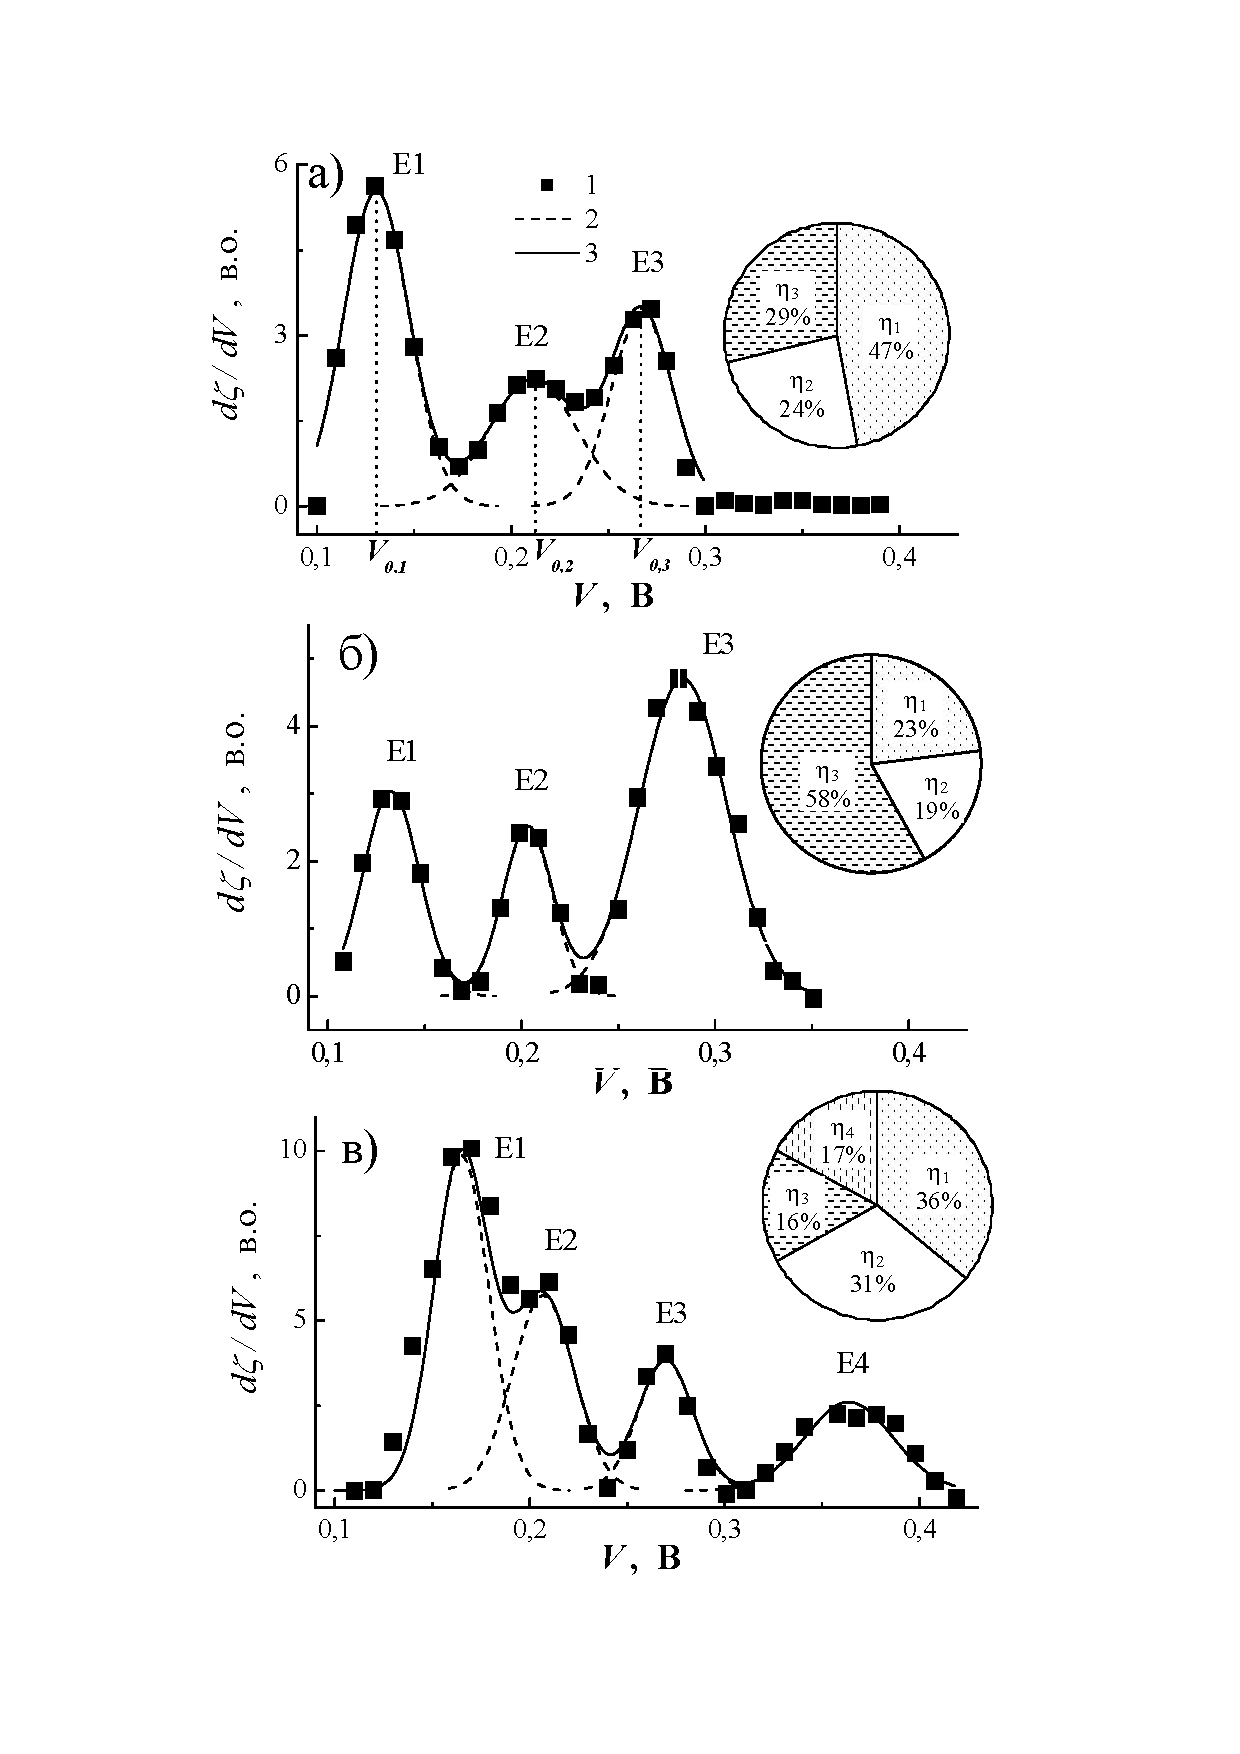
\includegraphics[width=0.6\textwidth]{figBul1}
\caption{\label{figBul1}
Польова залежність похідної диференційного показника нахилу ВАХ за відсутності УЗН (а)
та за його наявності (U--L26t, $W_\mathtt{US}=0,1$~Вт/см$^2$ та U--L4t,  $W_\mathtt{US}=0,25$~Вт/см$^2$ для б та в, відповідно).
1 --- точки, отримані після диференціювання експериментальних ВАХ,
2 --- гаусіани, якими апроксимувалися максимуми,
3 --- сума всіх гаусіан.
Зразок SC11A.
Справа біля кривих наведено діаграми питомих внесків $\eta_i$ кожного з максимумів у загальну криву.
}%
\end{figure}


\begin{table}
\caption{\label{tabBulEtUSL}Порівняння отриманих значень енергій активації глибоких рівнів та літературних даних.
}
\center
\begin{tabular}{|c|c|c|c|c|c|c|c|}
\hline
\multicolumn{5}{|c|}{Отримані результати}&\multicolumn{3}{c|}{Літературні дані}\\ \hline
&\multicolumn{2}{c|}{SC11A}&\multicolumn{2}{c|}{SC3}&&&\\ \cline{2-5}
Рівень&без УЗ&УЗН&без УЗ&УЗН&$E_c-E_t$,&Тип&Джерело\\ \cline{2-5}
&\multicolumn{4}{c|}{$(E_c-E_t)$, $\pm0,01$~еВ}&еВ&дефекту&\\
\hhline{========}
Е1&0,48&0,47&0,48&0,48&0,475&COV$_2$&\cite{Lugakov}\\\cline{6-8}
&&&&&0,50--0,52&дисл.&\cite{Edis:Ogawa,Edis:Omling,Kittler2003}\\ \hline
Е11&---&---&0,46&0,46&0,46&V$_3$&\cite{V3:PRB2012,V3:Markevich}\\ \cline{6-8}
&&&&&0,46&V$_2$O&\cite{V2:JAP2014}\\ \cline{6-8}
&&&&&0,46&V$_3$O&\cite{V3:Markevich}\\ \hline
Е2&0,44&0,425&0,43&0,42&0,42--0,46&VP$_s$&\cite{VI:Luc,Kuchinskii,Karazh,Ecentre:2005}\\ \cline{6-8}
&&&&&0,43&дисл.&\cite{SiO:Vanhell}\\ \cline{6-8}
&&&&&0,43--0,44&V$_2$&\cite{V2:JAP2014,V2:PRB2002}\\ \cline{6-8}
&&&&&0,43&Fe$_i$B$_s$$^\mathtt{orth}$&\cite{FeB:PhysRevB49,Istratov1999}\\ \cline{6-8}
&&&&&0,45&Fe$_i$O$_i$&\cite{FeO}\\ \cline{6-8}
&&&&&0,43--0,44&Si$_i$&\cite{VI:Luc,Si:Sii}\\ \hline
Е3&0,40&0,40&0,40&0,39&0,41&BO$_\mathtt{SRC}$&\cite{LIDRev,LIDRev2,Rein,LID:SchmidtJMR}\\ \cline{6-8}
&&&&&0,41--0,43&SiO$_x$&\cite{SiO:Mchedlidze,SiO:Vanhell,SiO:Chan}\\ \cline{6-8}
&&&&&0,39&V&\cite{MSER55}\\ \hline
Е4&---&0,37&0,37&0,355&0,36--0,38&BO$_\mathtt{FRC}$& \cite{LIDRev2,BOSingle:SEMSS2017}\\ \cline{6-8}
&&&&&0,37&B$_i$&\cite{Lugakov}\\ \cline{6-8}
&&&&&0,34--0,36&V$_3$&\cite{V3:PRB2012,V3:Markevich}\\ \cline{6-8}
&&&&&0,34&V$_3$O&\cite{V3:Markevich}\\ \cline{6-8}
&&&&&0,37--0,39&дисл.&\cite{PhysRevB56:10208,kveder2008,SiO:Hwang,disl10:Isakova,Kittler2003}\\ \cline{6-8}
&&&&&0,36; 0,39&Si$_i$&\cite{MSER55,Si:Sii}\\ \hline
\end{tabular}
\end{table}



Під час УЗН картина максимумів змінюється --- див. Рис.~\ref{figBul1},б та Рис.~\ref{figBul1},в.
А саме, змінюються співвідношення площ під максимумами (внески в рекомбінацію різних ГР),
відбувається незначний зсув положення максимумів (зміна енергії активації ГР),
змінюється кількість максимумів (проявляються новий ГР).
Зокрема, при U--L4t та U--L8t з'являється сигнал ще від одного ГР,
позначеного Е4, для якого $E_c-E_{t,i}=(0,37\pm0,01)$~еВ.
Більш детально АІ зміни розглянуті в параграфі~\ref{sbBul3}.


Результати, отримані для SC3, наведено на Рис.~\ref{figBul2} та в Таблиці~\ref{tabBulEtUSL}.
Видно, що в цьому випадку картина більш складна, ніж для SC11A:
навіть за відсутності УЗН присутній максимум Е4 та, крім того,
спостерігається ще один максимум, позначений Е11, який пов'язаний з рівнем $E_c-E_{t,i}=(0,46\pm0,01)$~еВ.
Характер АІ змін для SC3, загалом, збігається з виявленими в SC11A ефектами.




\begin{figure}
\center
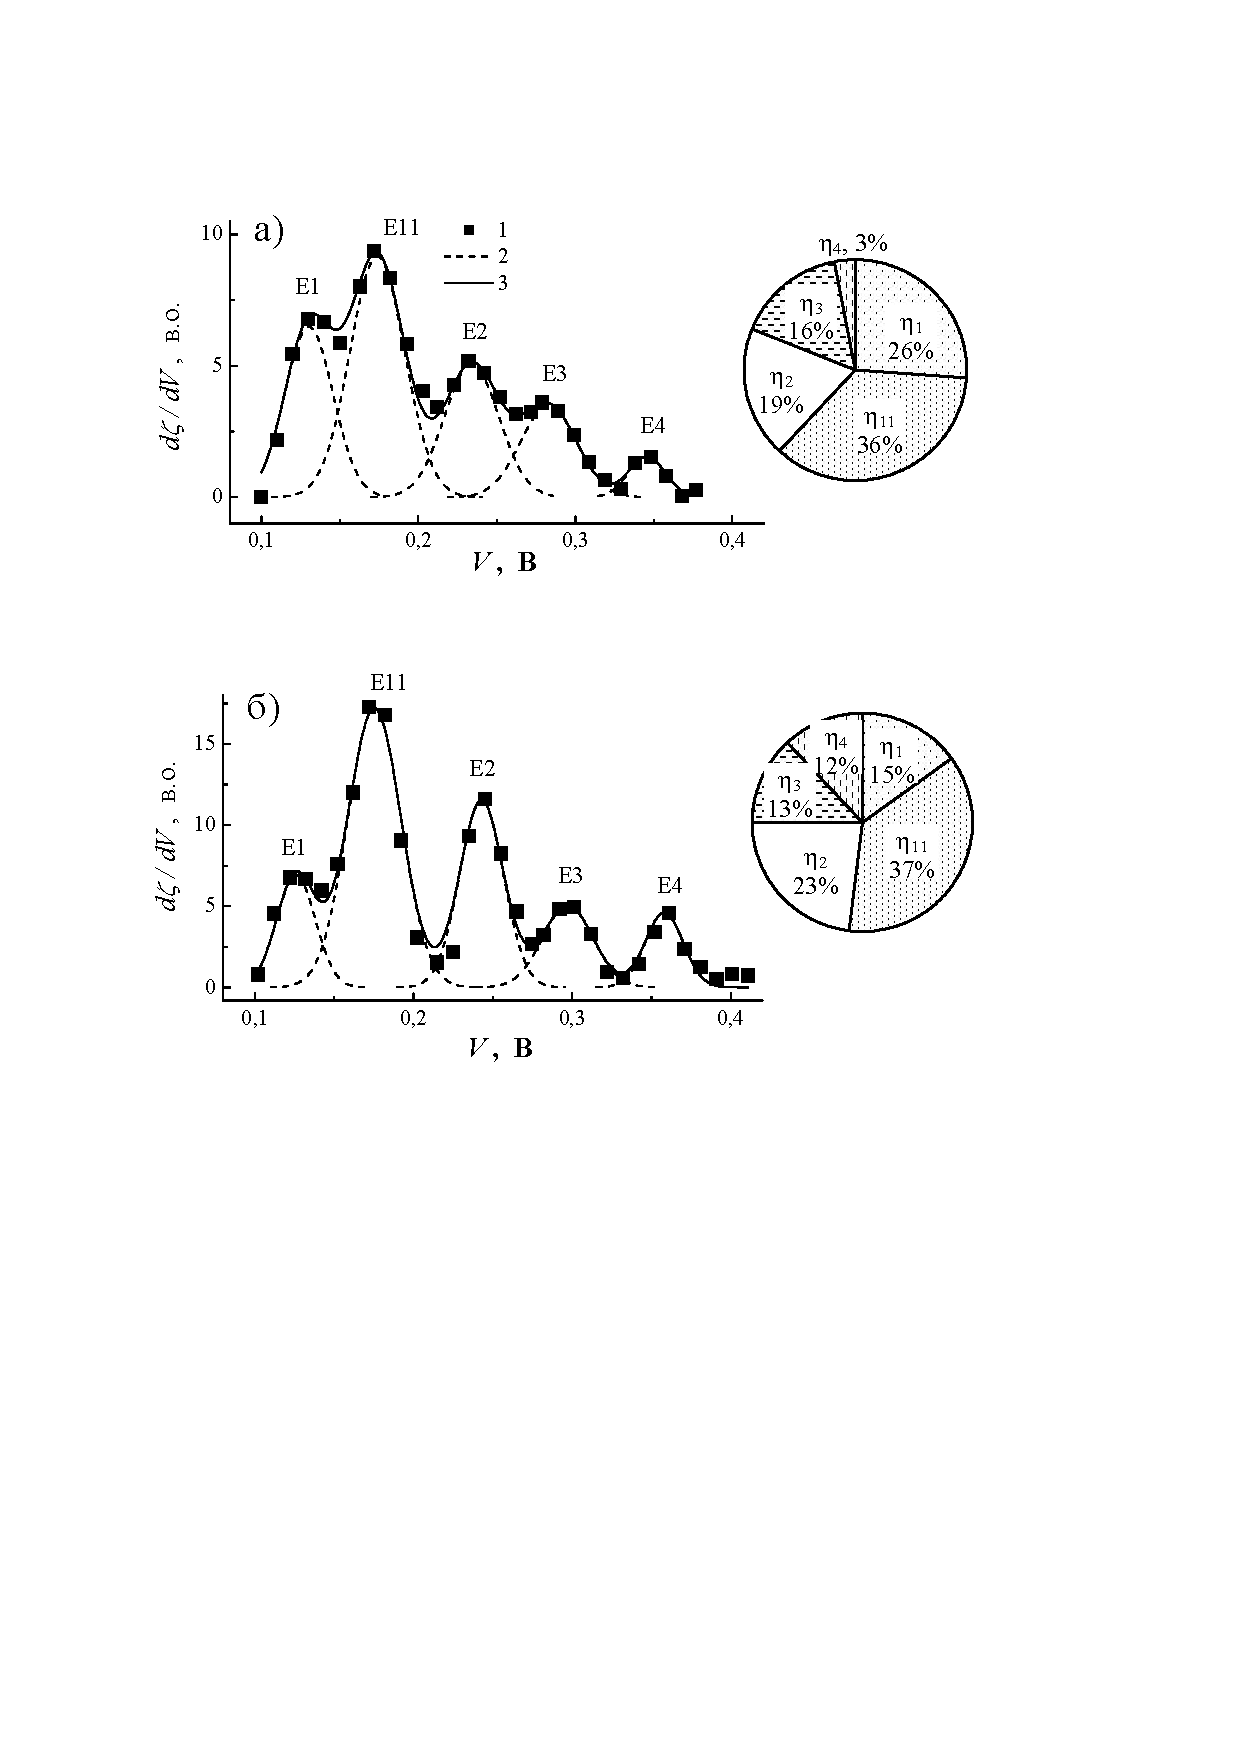
\includegraphics[width=1.0\textwidth]{figBul2}
\caption{\label{figBul2}
Польова залежність похідної диференційного показника нахилу ВАХ за відсутності УЗН (а)
та за його наявності (U--L4t,  $W_\mathtt{US}=0,60$~Вт/см$^2$, б).
1 --- точки, отримані після диференціювання експериментальних ВАХ,
2 --- гаусіани, якими апроксимувалися максимуми,
3 --- сума всіх гаусіан.
Зразок SC3.
Справа біля кривих наведено діаграми питомих внесків $\eta_i$ кожного з максимумів у загальну криву.
}%
\end{figure}

Загалом, в літературі відомо чимало дефектів в кристалах кремнію, енергетичні рівні яких знаходяться на відстані
$0,35\div0,50$~еВ від дна зони провідності.
Відомі значення енергій активації та відповідні конфігурації дефектів наведено в правій частині Таблиці~\ref{tabBulEtUSL}.
Спираючись на отримані величини $E_c-E_t$, технологію виготовлення зразків та літературні дані
визначемо, які конкретні дефекти можуть бути співставлені рівням Е1--Е4.

Досліджені структури містять несиметричний $n^+$--$p$ перехід і ОПЗ знаходиться практично повністю в області з дірковою провідністю.
Отже, переважно рекомбінація буде відбуватися за участю тих центрів, які мають донорний характер.
Як вже згадувалося, легування $n$--шару здійснювалось шляхом іонної імплантації фосфору.
В таких структурах, як в $n$--, так і в $p$--областях, можуть часто зустрічатися так званий Е--центр,
тобто комплекс вакансії та заміщуючого атома фосфору VP$_s$.
Цьому дефекту відповідає  рівень з енергетичним положенням $E_t=E_c-(0,42\div0,46)$~еВ \cite{VI:Luc,Karazh,Kuchinskii,Ecentre:2005}, що близько до параметрів центру Е2.
Проте відомо \cite{Kuchinskii,Ecentre:2005}, що цей рівень є акцепторним, йому відповідає зарядовий стан  $(-/0)$ і він є рекомбінаційно--активним переважно в $n$--Si.
Тому вважаємо, що Е--центр не відповідає за появу рівня Е2.
Після імплантації та відпалу атоми фосфору не зустрічаються у складі міжвузлових комплексів \cite{ChelyadFTT} і тому подібні дефекти ми також виключимо з розгляду.

Іншими типовими дефектами, які виникають внаслідок іонного опромінення є різноманітні
вакансійні комплекси.
Наприклад, енергія активації рівня Е1 0,48~еВ достатньо близька до положення рівня
комплексу COV$_2$  $E_t=E_c-0,475$~еВ \cite{Lugakov}.
Проте цей центр спостерігався в $n$--Si, опроміненому або електронами, або $\gamma$--квантами \cite{Lugakov} і тому його поява в досліджених структурах малоймовірна.

За своїм енергетичним положенням у верхній частині
забороненої зони рівні дивакансії $(-/0)$ $E_c-(0,43\div0,44)$~еВ \cite{V2:JAP2014,V2:PRB2002},
вакансії $(2-/-)$ $E_c-0,39$~еВ \cite{MSER55},
тривакансії $(2-/-)$ $E_c-(0,34\div0,36)$~еВ та $(-/0)$ $E_c-0,46$~еВ \cite{V3:PRB2012,V3:Markevich}
можуть відповідати центрам Е2, Е3, Е4 та Е11.
Проте всі вони є акцепторними (одно-- чи двозарядними) і тому також не можуть проявлятися
в наших експериментах.
Подібна властивість, коли акцепторні рівні знаходяться у верхній половині $E_g$,
а донорні --- в нижній, характерна і для різноманітних мультивакансій V$_n$ ($n>3$) \cite{Si:multiV}.

Утворені після імплантації фосфору вакансії є достатньо рухливими і в Cz--Si
утворюють (особливо після відпалу) комплекси з киснем \cite{V2toV2O}.
Глибина залягання рівня Е4 близька до розташування стану V$_3$O $(2-/-)$ (0,34~еВ нижче дна зона провідності \cite{V3:Markevich}),
а рівня Е11 --- до станів V$_3$O $(-/0)$ ($E_c-0,46$~еВ \cite{V3:Markevich})
та V$_2$O $(2-/-)$ ($E_c-0,46$~еВ \cite{V2:JAP2014}).
Проте ці рівні також акцепторні.
Таким чином, участь комплексів, пов'язаних з вакансіями, в утворенні
піків на залежності $\partial \zeta/ \partial V $, зв'язаних з рівнями Е1--Е4 може бути виключена.

При іонній імплантації кремнію, попередньо легованого бором,
у значній кількості утворюються власні міжвузольні дефекти та B$_i$.
Положення рівня міжвузольного бору $E_c-0,37$~еВ \cite{Bi:Harris} близьке до  енергії активації Е4.
Тоді як з Si$_i$ пов'язують декілька рівнів: $E_c-0,36$~еВ \cite{MSER55},
$E_c-0,39$~еВ \cite{MSER55,Si:Sii}, $E_c-0,43$~еВ \cite{Si:Sii} та
$E_c-0,44$~еВ \cite{VI:Luc}.
Зауважимо, що перший з них є нестабільним і спостерігається лише після опромінення при низьких температурах \cite{MSER55}.
Ці характеристики близькі до енергій активацій рівнів Е2 та Е4.

Раніше, у параграфі~\ref{sbDefectType}, вже згадувалося, що
типовими порушеннями в Cz--Si:B є ВО дефекти, кисневмісні преципітати та домішки заліза.
До речі, утворення КП також супруводжується емісією Si$_i$ \cite{MSER13}:
\begin{equation*}\label{eqSiO}
  2\,x\,\mbox{O}_i+y\,\mbox{Si}_s\leftrightarrows x\,\mbox{SiO}_2+(y-x)\,\mbox{Si}_i\,.
\end{equation*}
З самими КП пов'язують рівні, розташовані на відстані 0,41--0,43~еВ від дна зони провідності \cite{SiO:Mchedlidze,SiO:Vanhell,SiO:Chan}, що, враховуючи  $\delta_{Et}$, достатньо близько до енергії активації Е3.

Подібне розташування ($E_t=E_c-0,41$~еВ, \cite{LIDRev,LIDRev2,BO3i,Rein,LID:SchmidtJMR}) характерне і для ВО--дефекту.
Як відомо, ці центри утворюються внаслідок інжекції носіїв,
їх конфігурація визначена не точно, зокрема в літературі пропонується,
що це можуть бути комплекси B$_i$B$_s$O$_i$, B$_s$Si$_i$\cite{LIDRev} або
B$_i$O$_{3i}$ \cite{BO3i}.
Проте серед ВО виділяють дефекти,
що утворюються швидко (FRC, fast--formed recombination center)
та повільно (SRC, slow--formed recombination center).
Означений вище рівень відносять до SRC--форми,
тоді як  BO$_\mathtt{FRC}$ характеризується рівнем $E_c-(0,36\div0,38)$~еВ \cite{LIDRev2,BOSingle:SEMSS2017}, який
також потрапляє у діапазон, що нас цікавить (рівень Е4).

При утворенні КП, окрім власних міжвузольних атомів, для зняття механічних напруг також утворюються дислокації та дефекти пакування.
Серед останніх виділяють так звані OSFR--дефекти (oxidization induced stacking--faults ring), оточені кільцевими частковими дислокаціями \cite{MSER74,MSER28}.

З дислокаціями в кремнії пов'язують цілий ряд енергетичних рівнів, зокрема
$E_c-(0,37\div0,39)$~еВ \cite{PhysRevB56:10208,kveder2008,SiO:Hwang,disl10:Isakova,Kittler2003},
$E_c-0,43$~еВ \cite{PhysRevB56:10208,SiO:Vanhell}
$E_c-(0,50\div0,52)$~еВ \cite{Edis:Ogawa,Edis:Omling,Kittler2003},
близькі за параметрами до Е4, Е2 та Е1, відповідно.

Щодо рівнів, пов'язаних з дефектами, які містять залізо, то у діапазоні енергій, який розглядається,
знаходяться рівні $E_c-45$~еВ, пов'язаний з комплексом FeO \cite{FeO},
та $E_c-43$~еВ, що співставляється з парою Fe$_i$B$_s$, що має ромбічну симетрію \cite{FeB:PhysRevB49,Istratov1999}.
Як видно з даних Таблиці~\ref{tabBulEtUSL}, ці значення співрозмірні з енергією активації Е2.

Таким чином, серед типових дефектів у кремнієвих структурах є декілька кандидатів,
які можуть біти відповідальними за появу рівнів Е1, Е2, Е3 та Е4 та, фактично, жодного на роль Е11.
У наступному параграфі, спираючись на виявлені АІ ефекти, це коло буде звужене (розширене).

\subsection{Акусто--індуковані зміни в системі рекомбінаційних центрів\label{sbBul3}}

Як вже зазначалося, в умовах УЗН залежність $\partial \zeta/ \partial V = f (V)$ змінювалась.
Основні результати щодо впливу УЗН на рекомбінаційні рівні в SC11A та SC3 наведено
на Рис.~\ref{figEta1} та Рис.~\ref{figEta2}, відповідно.
Узагальнюючи представлені результати зазначимо, що


\begin{figure}
\center
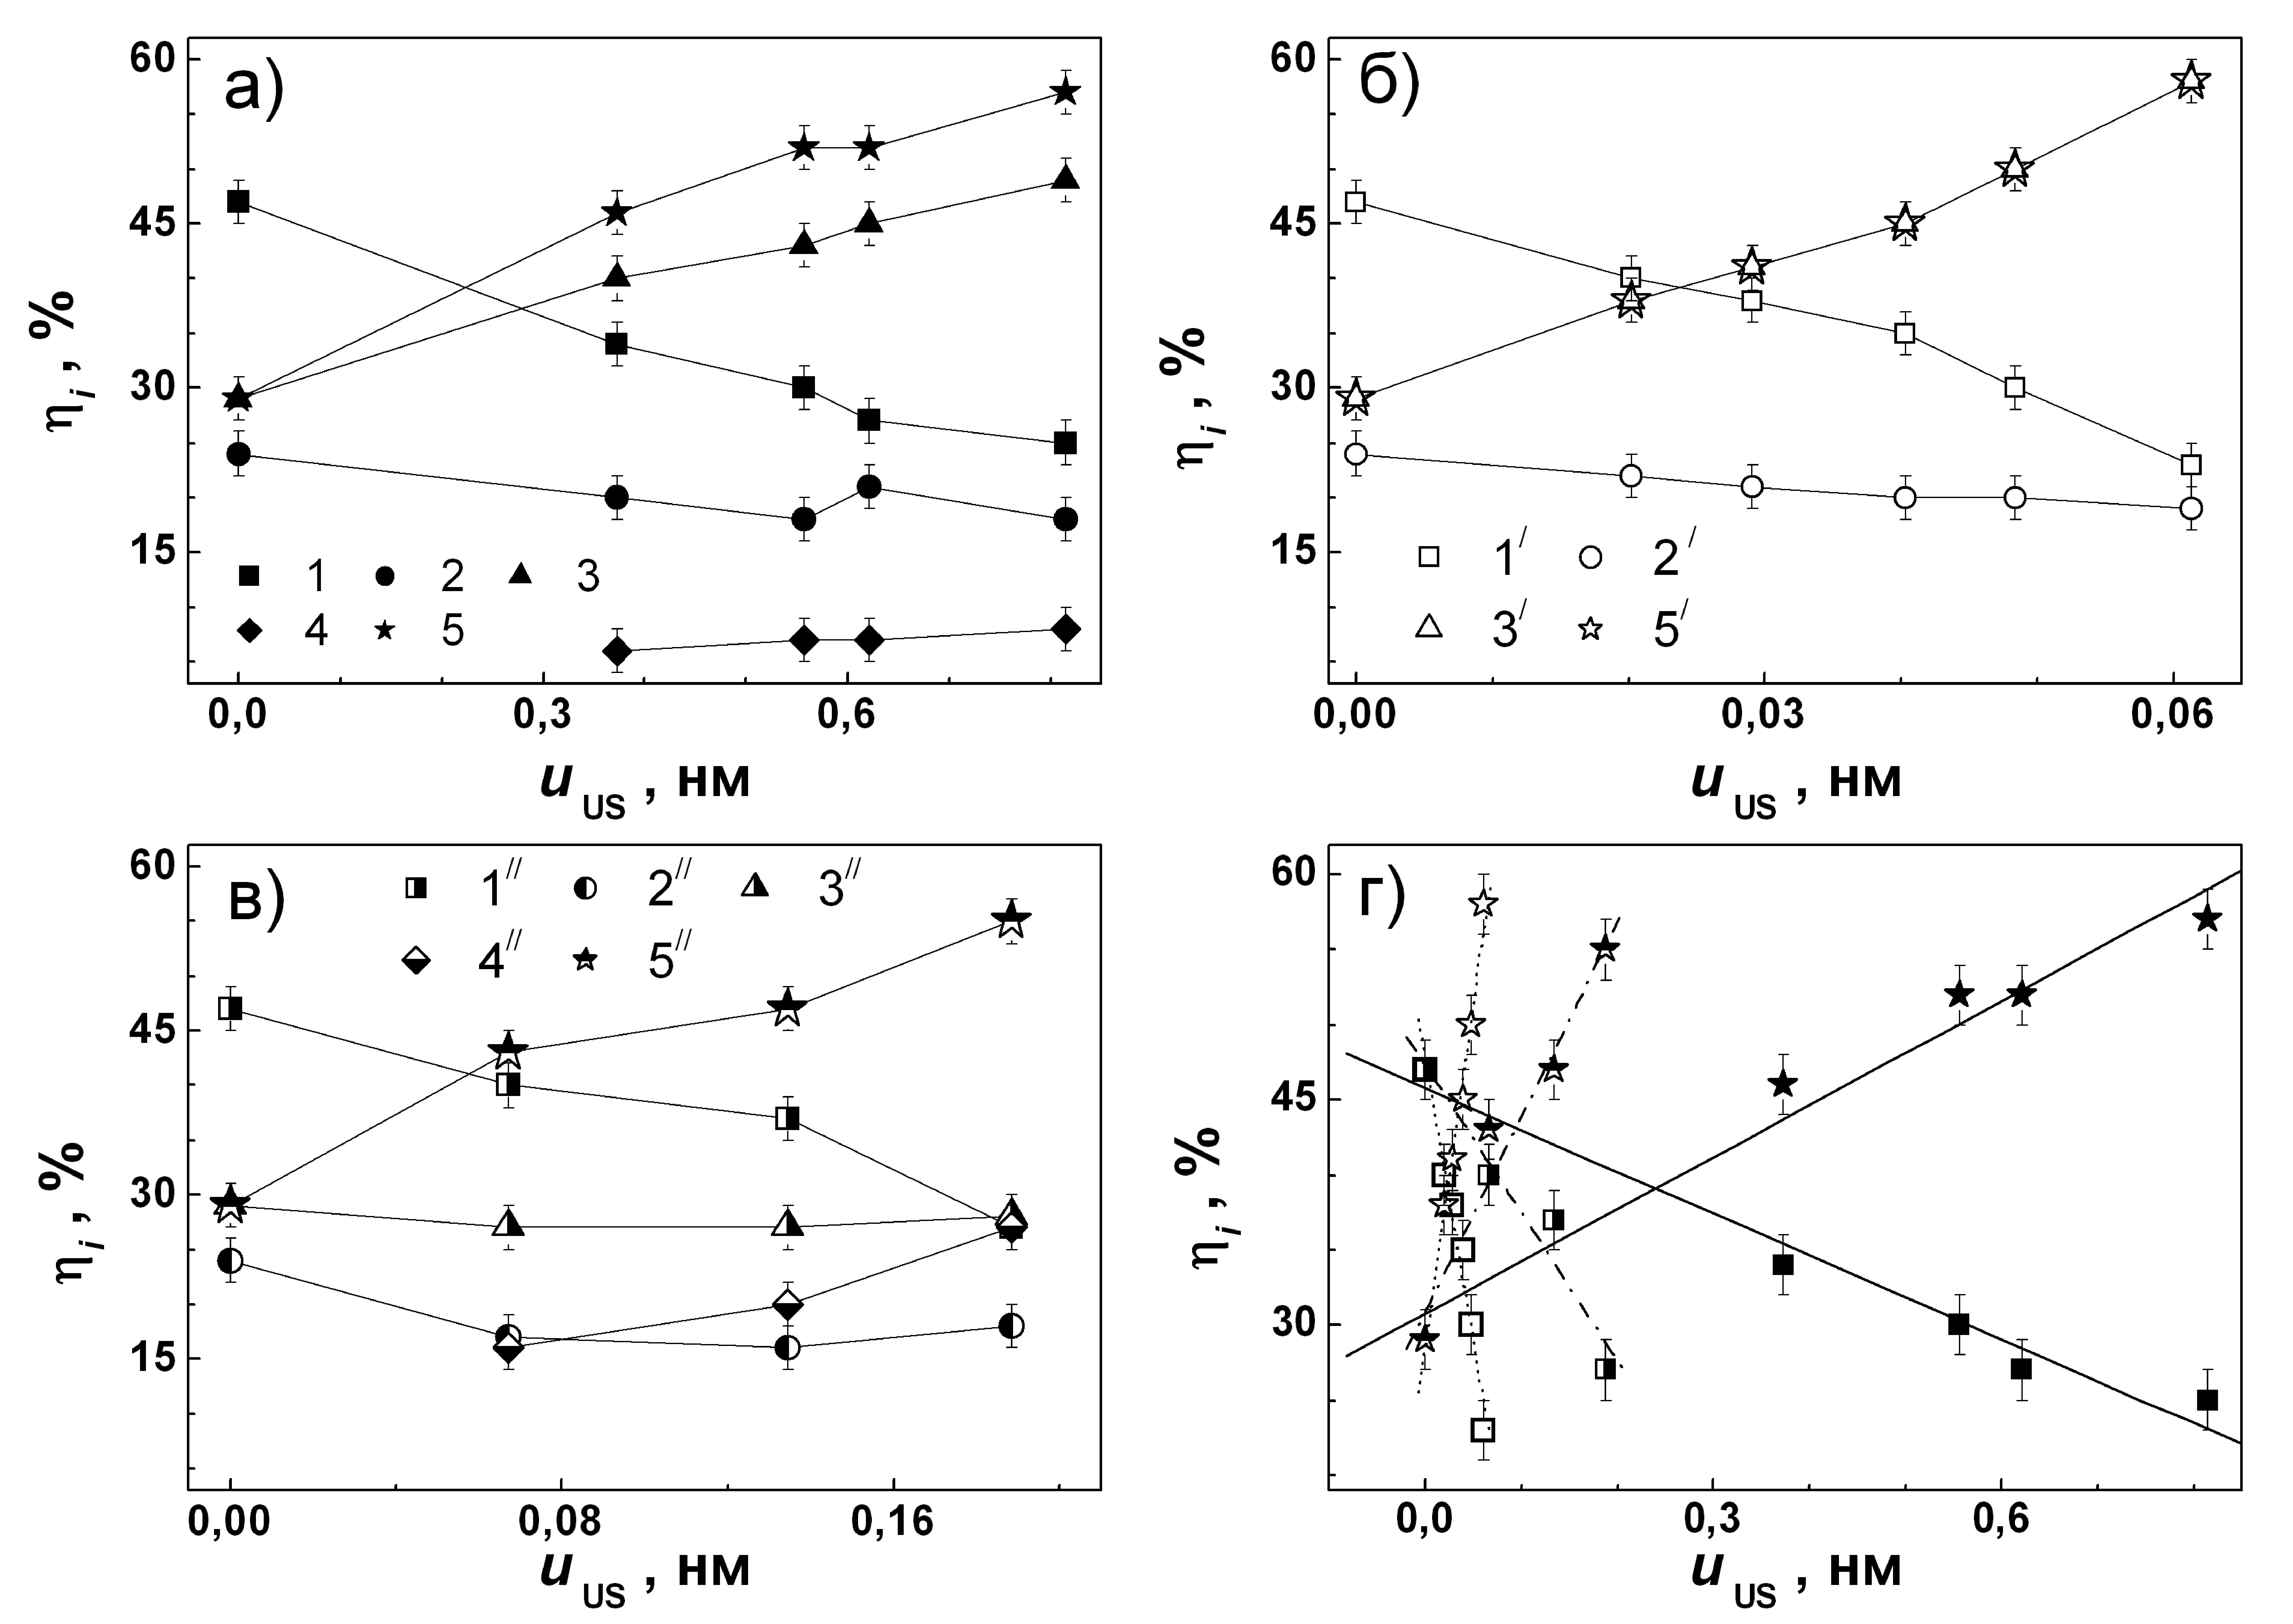
\includegraphics[width=1.0\textwidth]{figEta1}
\caption{\label{figEta1}
Залежність питомих внесків у загальну рекомбінацію рівнів
Е1 (криві 1, 1$^{\prime}$ та 1$^{\prime\prime}$, квадрати),
Е2 (криві 2, 2$^{\prime}$ та 2$^{\prime\prime}$, кола),
Е3 (криві 3, 3$^{\prime}$ та 3$^{\prime\prime}$, трикутники)
та Е4 (криві 4, та 4$^{\prime\prime}$, ромби),
а також сумарного внеску
Е3 та Е4 (криві 5, 5$^{\prime}$ та 5$^{\prime\prime}$, зірки)
від амплітуди зміщень атомів
при U--L4t (а, г, заповнені точки),
U--L26t (б, г, порожні точки),
U--L8t (в, г, напівзаповнені точки).
Зразок SC11A.
На а--в лінії наведені лише для зручності,
на г --- лінії результат лінійної апроксимації.
}%
\end{figure}

\begin{figure}
\center
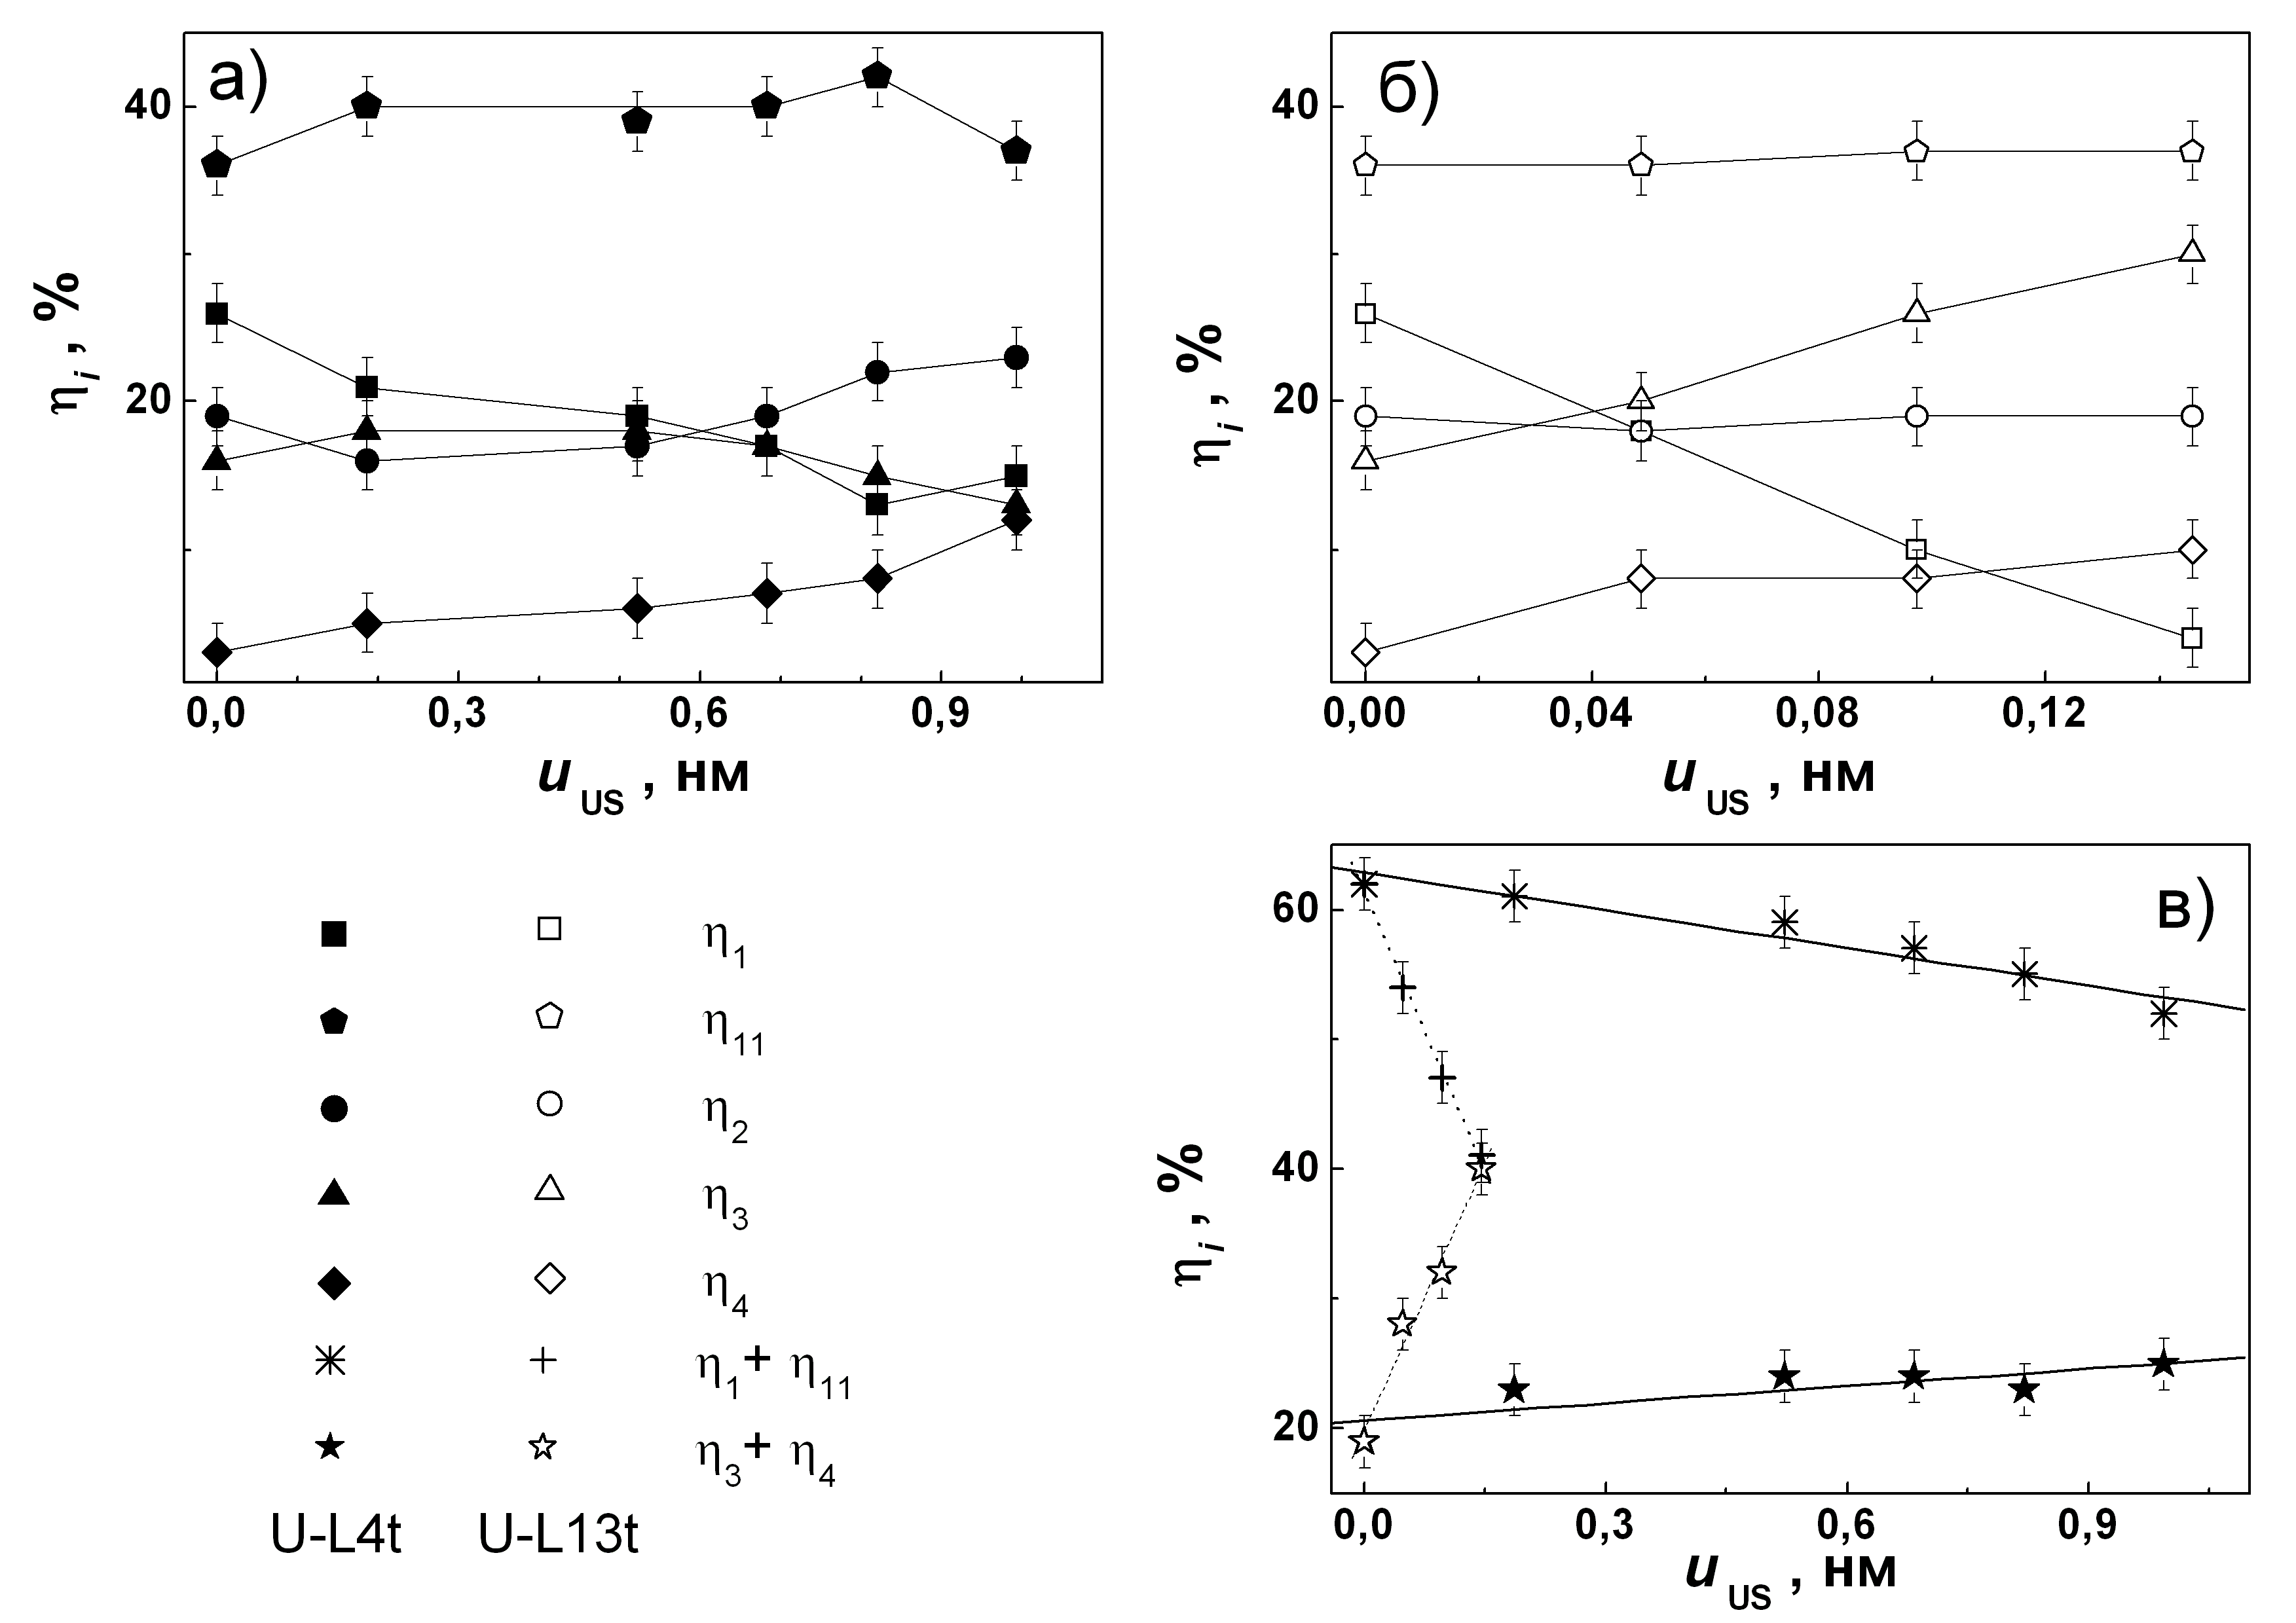
\includegraphics[width=1.0\textwidth]{figEta2}
\caption{\label{figEta2}
Залежність питомих внесків у загальну рекомбінацію рівнів
Е1 (квадрати),
Е11 (п'ятикутники),
Е2 (кола),
Е3 (трикутники)
та Е4 (ромби),
а також сумарного внеску
Е1 та Е11 (хрести) і
Е3 та Е4 (зірки)
від амплітуди зміщень атомів
при U--L4t (а, в, заповнені точки) та
U--L13t (б, в, порожні точки).
Зразок SC3.
На а--в лінії наведені лише для зручності,
на г --- лінії результат лінійної апроксимації.
}%
\end{figure}

\begin{enumerate}[label=\asbuk*),leftmargin=0em,itemindent=1.5em]
\item зі збільшенням інтенсивності УЗ збільшується роль у рекомбінаційних процесах рівнів, розташованих ближче до дня зона провідності; зокрема збільшується внесок рівня Е3 та зменшується внесок рівня Е1, причому залежності показників питомого внеску рівнів від амплітуди зміщень атомів у  АХ ($\eta_i\sim U_\mathtt{US}$);
\item АІ зміни відбуваються більш ефективно при підвищенні частоти УЗН --- див Рис.~\ref{figEta1},г та Рис.~\ref{figEta2},в;
\item в умовах УЗН в зразку SC11A з'являється сигнал від ще одного ГР (Е4), тоді як в SC3 відповідний сигнал наявний і за відсутності пружних коливань; внесок цього рівня $\eta_4$ збільшується зі зростанням $U_\mathtt{US}$;
\item спостерігається незначний, 0,010--0,015~еВ, зсув положення рівнів ближче до дна зони провідності; зауважимо що величина зсуву співрозмірна з похибкою визначення енергії активації і причиною виокремлення цього ефекту є лише постійність його знаку для всіх зразків та режимів.
\end{enumerate}

Зупинимось на причинах АІ появи рівня Е4.
У випадку, коли цей рівень пов'язаний з міжвузольним атомом бору, можна запропонувати наступним механізм цього ефекту.
При УЗН може відбуватися звільнення власних міжвузольних атомів, захоплених дислокаційними петлями поблизу $p$--$n$ переходу (можливість існування значної кількості Si$_i$ та дислокацій згадувалась у попередньому параграфі);
після цього Si$_i$ дифундують в глибину $p$--області, де витісняють легуючі атоми В з вузлів за механізмом Воткінса.
Проте
а)~при такому варіанті незрозумілим залишається зникнення сигналу від Е4 в SC11A після припинення УЗН (всі виявлені ефекти є оборотними);
б)~В$_i$ є центром з від'ємною кореляційною енергією, його донорний рівень $E_t=E_c-0,13$~еВ \cite{Bi:Harris} знаходиться ближче до $E_c$, тому ймовірність спостереження акцепторного рівня
$E_t=E_c-0,37$~еВ в $p$--Si дуже мала;
в)~дефект відпалюється вже при температурах 240--250~K, перетворюючись на комплекс B$_i$O$_i$ ($E_c-0,23$~еВ) \cite{PhysRevB94}.
Як наслідок, подібний механізм, як і те, що Е4 пов'язаний саме з В$_i$, видається малоймовірним.

Інший цікавий з точки зору АДВ варіант появи Е4 полягає в тому, що в умовах УЗН відбувається
перебудова ВО дефекту з однієї конфігурації в іншу: $\mbox{BO}_\mathtt{CRC} \rightarrow \mbox{BO}_\mathtt{FRC}$.
Тобто і Е3, і Е4 відносяться до одного й того ж ВО дефекту у різних конфігураціях,
УЗН викликає збільшення частки дефектів у конфігурації  BO$_\mathtt{FRC}$, що призводить до появи відповідного максимуму (SC11A) або його підсилення (SC3).
Те, що сигнал від Е4 присутній у SC3 і до УЗН свідчить просто про нерівномірність розподілу цих дефектів по пластині.
Якщо Е3 та Е4 відповідають двом станам ВО, то доцільно розглядати суму $\eta_3+\eta_4$ як показник внеску цього дефекту в загальну рекомбінацію, що і зроблено на рисунках.
Отримані залежності вказуються, що в цілому внесок ВО комплексу в рекомбінацію при дії пружних коливань зростає.
Як було розглянуто раніше (параграф~\ref{sbAEDefect}), згідно з моделлю акусто--активного комплексу найбільш очікуваною АДВ є для системи, складові якої характеризуються різним за знаком надлишковим об'ємом.
В цілому, ВО задовольняє цій умові для конфігурацій, що містять заміщуючий атом бору (B$_i$B$_s$O$_i$ тв B$_s$Si$_i$).
Дійсно, так як ковалентний радіус бору дорівнює 0,8~{\AA}, а кремнію -- 1,18~{\AA},
то $\Delta\Omega_d\,(\mbox{B}_s)<0$,
тоді як для міжвузольних компонент $\Delta\Omega_d>0$.

На жаль, від такої стрункої картини доведеться також відмовитися.
По--перше, з недавнього часу в літературі наводяться докази того, що не існує двох
різних конфігурацій  (двох різних дефектів) FRC та SRC \cite{BOSingle:Voronkov,BO3i,BOSingle:SEMSS2017,Kim},
а отже АІ перехід $\mbox{BO}_\mathtt{CRC} \rightarrow \mbox{BO}_\mathtt{FRC}$ неможливий.
По--друге, згідно з результатами, викладеними в параграфі~\ref{sbDefectType},
в досліджуваних зразках ВО центри не впливають на рекомбінацію,
а отже ні Е3, ні Е4 з ВО дефектами не зв'язані.


На наш погляд, правильна картина АІ появи E4 наступна.
Відомо, що на периферійних ділянках напівпровідникових пластин концентрація дефектів вища,
ніж для центральних.
В нашому випадку про це, зокрема, свідчить менше значення шунтуючого опору в ($\sim2\cdot10^{3}$~Ом при кімнатній температурі) порівняно з SC11А ($\sim2\cdot10^{4}$~Ом).
В досліджуваних структурах шунтуючий опір визначається дислокаціями, які перпендикулярні до площини $p$--$n$ переходу, причому в умовах УЗН їх рекомбінаційна активність зростає ($R_{sh}$ зменшується) --- детально це описано в параграфі~\ref{sbRsh}.
Якщо припустити, що Е4 зв'язаний з дислокаціями (див. Таблицю~\ref{tabBulEtUSL}), яких більше в SC3, то зрозумілим стає наявність відповідного максимуму в цьому зразку без УЗН і зростання $\eta_4$ при УЗН.

Щодо рівня Е3 (для якого $\eta_3$ також збільшується при поширенні АХ),
то він має бути пов'язаний з КП SiO$_x$.
Дійсно, згідно з результатами, представленими в параграфах \ref{sbQNR} та \ref{sbDefectType},
саме кисневмісні преципітати наявні в досліджених структурах і підвищують свою рекомбінаційну активність під дією УЗ.

Повертаючись до співставлення виявлених рівнів з конкретними дефектами зауважимо,
що Е1 може бути пов'язаний з OSFR та відповідними частковими дислокаціями.
Відомо, що при захопленні дислокаціями домішок, їх рекомбінаційна активність
збільшується у декілька разів \cite{disl10:Kveder,Kittler2003}.
При УЗН відбувається часткове звільнення цих захоплених атомів, що і викликає
зменшення  $\eta_1$.
Крім того, в літературі описано уширення  лінії дислокаційної люмінесценції внаслідок захоплення домішки  \cite{PhysRevB56:10208}.
Більш висока концентрація домішок в SC3, у тому числі і захоплених на дислокаційні петлі,
на нашу думку і викликає наявність в діапазоні $E_c-(0,46\div0,48)$~еВ двох рівнів (Е1 та Е11),
внесок яких в рекомбінацію суттєво вищий, ніж в SC11А --- див. Рис.~\ref{figBul1} та Рис.~\ref{figBul2}.
Отже, внесок цих рівнів в рекомбінаційні процеси також можна розглядати разом ($\eta_1+\eta_{11}$, див. Рис.~\ref{figEta2}).

В параграфі \ref{sbDefectType} також було показано, що в ОПЗ присутні також домішкові атоми заліза.
Саме з ними і пов'язаний рівень Е2.
Вибираючи між Fe$_i$B$_s$ та Fe$_i$O$_i$ (див. Таблицю~\ref{tabBulEtUSL}), врахуємо наступне.
Звичайно, найчастіше як рекомбінаційний центр розглядають пару залізо--бор,
проте в літературі показано, що в $n^+-p$ переходах активними можуть бути і інші
залізовмісні пастки \cite{TeimurazPSS,TeimurazJAP}.
Пара  Fe$_i$B$_s$ є бістабільною, може перебувати в двох конфігураціях, які відрізняються відстанню між компонентами комплексу на симетрією (тригональна або ромбічна).
Рівень, з яким ми можемо пов'язати Е2, відповідає неосновному стану Fe$_i$B$_s^\mathtt{orth}$, тобто концентрація дефектів саме в цій конфігурації за рівноважних умов досить низька.
Нарешті, Е2 фактично не змінює свою рекомбінаційну активність в умовах УЗН.
$\Delta\Omega_d\,(\mbox{B}_s)<0$, то $\Delta\Omega_d\,(\mbox{O}_i)>0$, тобто комплекс
Fe$_i$B$_s$ є потенційно акусто--активним центром, тоді як для Fe$_i$O$_i$
$\Delta\Omega_d\,(\mbox{Fe}_i)\cdot\Delta\Omega_d\,(\mbox{O}_i)>0$.
Таким чином, кращим кандидатом для Е2 виглядає комплекс Fe$_i$O$_i$.

Наприкінці зауважимо, що зменшення енергії активації в кремнієвих структурах за умов
УЗ навантаження спостерігалося і раніше як для центрів, пов'язаних з дислокаціями \cite{KorotchFTP1996}, так і з точковими дефектами \cite{Korotchenkov1995}.
Причому в останньому випадку автори пов'язували ефект зі зміщенням домішки з рівноважного положення під дією механічної напруги, яка виникає під час поширення УЗ.


Таким чином, приведені результати підтверджують практичну перспективність динамічного акустичного керування властивостями напівпровідників та характеристиками приладів на їх основі.
Необхідно зауважити, що нерівноважний стан дефектів (в нашому випадку рекомбінаційних центрів), який виникає при появі нерівноважних носіїв заряду,
є важливим фактором підвищення ефективності АДВ загалом.
Саме в такому випадку додаткова коливальна деформація зовнішнього УЗ стає більш ефективним засобом керування характеристиками приладу.
Безумовно, питання фізичного механізму акустоіндукованих перетворень структури, конфігурації, зарядового стану дефектів у напівпровідниках потребують подальших досліджень.



\section{Особливості акусто--дефектної взаємодії в радіаційно--опромінених кремнієвих структурах з p--n переходом\label{Rad_SSC}}
У цьому параграфі викладено результати дослідження впливу УЗН на параметри опромінених кристалічних КСЕ.
Зрозуміло, що властивості таких структур визначаються, насамперед, дефектним складом.
Ефективність АДВ залежить від структури дефектів \cite{UST:Medvid} і
далеко не всі дефекти кристалічної структури кремнію є акусто--активними і здатні змінювати свою конфігурацію в умовах УЗН.
Одним з найбільш поширених та вивчених способів зміни дефектної підсистеми напівпровідників є опромінення.
З точки зору АДВ, з одного боку, виявлено \cite{YOlikh2007TPLr,Parchinskii2006r,Gorb2010,Podolian2012r}, що високоінтенсивна УЗО
здатна незворотнім чином змінювати властивості опромінених кремнієвих структур.
Цей ефект пов'язаний з АІ відпалом РД, насамперед точкових.
З іншого боку, опромінення може бути причиною появи оборотних АІ явищ \cite{YOlikh2006TPLr,YOlikhTPL2011r},
яка пов'язана з формуванням акусто--активних РД.
На жаль, експериментальному  дослідженню акусто--керованих ефектів в опромінених кремнієвих структурах присвячено достатньо небагато робіт.
Представлені результати частково доповнюють картину АДВ в подібних системах.
Зокрема проведено порівняння АІ ефектів, яки виникають при використанні опромінення різного типу (нейтронів та гамма--квантів),
а отже при появі дефектів різного типу.
Так як наслідки опромінення кремнію вивчені достатньо добре, то вдалося, зокрема, вирізнити
вплив УЗ на різні за типом РД.
Зразки та деталі радіаційного впливу описані у параграфі~\ref{SSC}.

Проводилось вимірювання ВАХ зразків у темряві за умов УЗН та без нього, спираючись на які було визначено параметри КСЕ.
Загалом процедура, за винятком об'єкту безпосереднього експериментального дослідження,
збігалася з описаною у параграфі~\ref{sbSSCMethod}.
Відмінності мали місце лише при отриманні результатів, наведених у параграфі \ref{sbNIsc},
але на його початку експериментальні деталі описані окремо.
На Рис.~\ref{figSSCIV2} наведено декілька прикладів виміряних кривих, які відображають
зміну форми ВАХ внаслідок опромінення.
Крім того, на рисунку за допомогою розривних ліній показано приклад розрахованих під час апроксимації внесків $I_{SCR}$, $I_{base}$ та $I_{sh}$
(див. формулу~(\ref{eqSSCIV})) у загальний струм.
На цьому рисунку, як і надалі, проводиться порівняння результатів,
отриманих для опромінених КСЕ, з даними для неопроміненого зразка SC11, параметри якого, зокрема величина шунтуючого опору,
схожі з параметрами SC4, SC8, SC12.
Так як при вивченні АІ ефектів в опромінених структурах використовувалися лише поперечні АХ,
то для порівняння наведено результати впливу на SC11 УЗН з таким самим типом хвиль.

\begin{figure}
\center
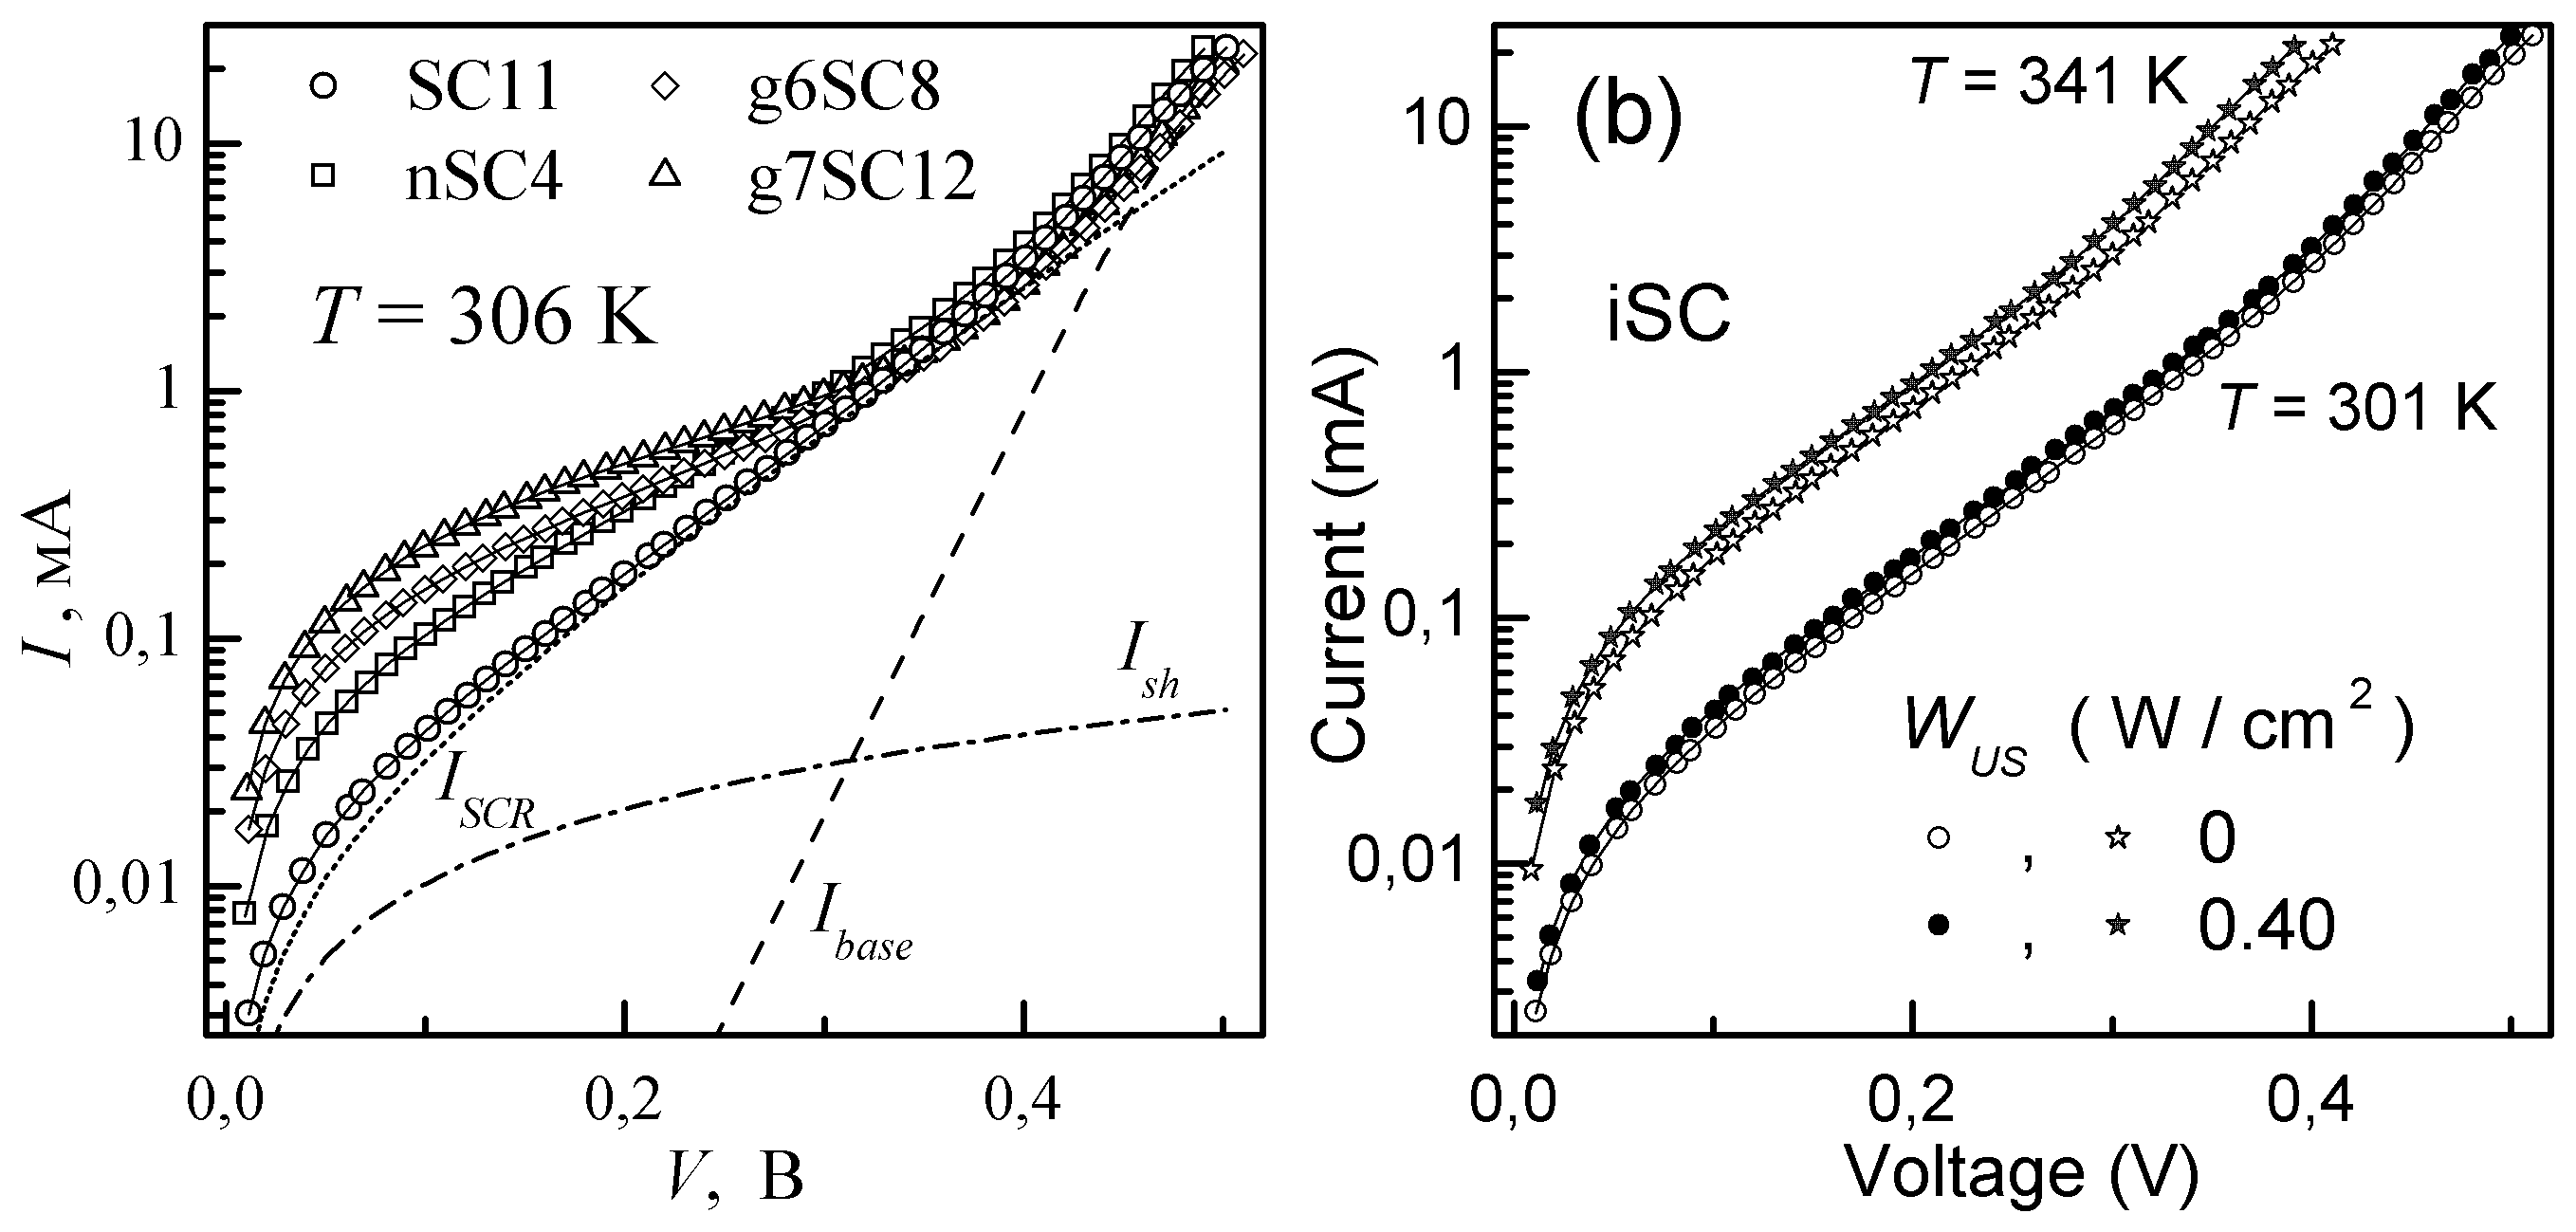
\includegraphics[width=0.6\textwidth]{figSSCIV2}%
\caption{\label{figSSCIV2}
Темнові ВАХ неопроміненого зразка (кола), нейтронно--опроміненого (квадрати) та $\gamma$-опроміненого (ромби та трикутники) виміряні при температурі 306~K без УЗН.
Точки відображають результати вимірів, лінії отримані шляхом апроксимації за формулами (\ref{eqSSCIV}) та (\ref{eqW}).
Штрихованою, пунктирною та штрих--пунктирною лініями показано розраховані складові повного струму, пов'язані з рекомбінаціяєю в КНО, в ОПЗ та шунтуючу складову, відповідно,
для неопроміненого зразка.
}%
\end{figure}



\subsection{Оцінка наслідків опромінення\label{sbRadDefCreate}}

При передбаченні структури РД, які утворюються внаслідок опромінення кристалів кремнію,
необхідно враховувати рівень та тип легування, концентрацію кисню та дозу.
В нашому випадку використовувалися зразки $p$--Si з концентрацією бору $\sim10^{15}$~cm$^{-3}$,
вирощені за методом Чохральського, зі значною концентрацією
кисню, $\sim7\times10^{17}$~см$^{-3}$ та достатньо низькі дози опромінення.
В цьому випадку очікується \cite{n:long,n:gamma,Moll:PhD}, що при нейтронному опроміненні будуть виникати
К--центри (пара міжвузольний вуглець--міжвузольний кремній, C$_i$O$_i$ ),
вакансійні кластери V$_n$ (дивакансії V$_2$, тривакансії V$_3$, ...) та
А--центри (пара вакансія--міжвузольний атом кисню, VO$_i$).
В той же час $\gamma$--промені мають викликати появу лише, переважно, C$_i$O$_i$ та VO$_i$ \cite{gamma:Stahl,Moll:PhD,gamma:Kolkr,A:Caracas}.
Відомо, що концентрація РД $N_{t,\mathtt{RD}}$ лінійно залежить від дози (флюєнсу) опромінення:
\begin{equation}
\label{eqNtRD}
    N_{t,\mathtt{RD}}=\vartheta^{D} D=\vartheta^{\Psi}\Psi \,,
\end{equation}
де $\vartheta^{D}$ ($\vartheta^{\Psi}$) --- швидкість введення (генерації) дефектів.
Запропоновані в літературі значення темпів генерації при опроміненні нейтронами $\vartheta_n$ та гамма--квантами $\vartheta_\gamma$
наведено в Таблиці~\ref{tabDefectNt}.
В цій же таблиці також наведені очікувані значення $N_{t,\mathtt{RD}}$ для досліджених зразків.

\begin{table}
\caption{\label{tabDefectNt}Швидкості введення та концентрації дефектів у досліджених зразках.
}
\center
\begin{tabular}{|c|c|c|c|c|c|c|}
\hline
Дефект&$\vartheta_n^{\Psi}$,  &$\vartheta_\gamma^{\Psi}$,&$\vartheta_\gamma^D$,&\multicolumn{3}{c|}{$N_{t,\mathtt{RD}}$, 10$^{11}$~см$^{-3}$}\\
\cline{5-7}
&см$^{-1}$ \cite{Moll:PhD}&см$^{-1}$ \cite{gamma:Kolkr}&рад$^{-1}$см$^{-3}$ \cite{gamma:Stahl}&nSC4&g6SC8&g7SC12\\
\hline
C$_i$O$_i$&1.38&4$\cdot$10$^{-4}$&6$\cdot$10$^5$&5,5&6&60\\ \hline
V$_2$&1,21&&3$\cdot$10$^4$&4,8&0,3&3\\ \hline
V$_3$&0,37&---&---&1,5&---&---\\ \hline
VO$_i$&0,52&4$\cdot$10$^{-4}$&7$\cdot$10$^5$&2&6--7&60--70\\\hline
\end{tabular}
\end{table}

У таблиці представлені дані лише для основних дефектів.
Окрім них при $\gamma$-- та нейтронному опроміненні кремнію можуть також утворюватися
а)~I$_p$ центри, пов'язані з міжвузольними атомами;
б)~бістабільні донори (BD-дефекти);
в)~пари міжвузольний бор--міжвозольний кремній (B$_i$O$_i$);
г)~пари міжвузольний вуглець--заміщуючий вуглець (C$_i$C$_s$).
Проте в досліджуваних зразках їх впливом можна знехтувати.
Так, утворення бістабільних донорів та I$_p$ центрів характеризується порівняно малою швидкістю введення.
Наприклад, як показують результати робіт \cite{n:gamma,BD:Fret}, в nSC4 та g7SC12 очікувана
концентрація BD дорівнює лише $(1\div2)\cdot10^{10}$~см$^{-3}$.
практично повна відсутність пар B$_i$O$_i$ пов'язана з невисокою концентрацією легуючого бору \cite{SiIntDef}.
Нарешті, відомо \cite{gamma:Kolkr,gamma:Stahl,n:long}, що формування комплексів C$_i$C$_s$ пригнічується у кристалах
з високою концентрацією кисню, зокрема вирощених за методом Чохральського.
Крім того  C$_i$C$_s$ не є рекомбінаційно--активним центром \cite{CiCs:Song}, а наше дослідження,
фактично, пов'язане з вивчення впливу УЗН на рекомбінаційні процеси в КСЕ.



\subsection{Область просторового заряду\label{sbSCR}}

Як вже згадувалося раніше, $n_{\mathrm{id}}$ та $\tau_{g}$ є саме тими параметрами ВАХ, які відображають рекомбінаційні процеси в
області просторового заряду.
Отримані температурні залежності фактору неідеальності та часу життя в ОПЗ наведено на Рис.~\ref{fignRD} та Fig.~\ref{figTAUgRD}, відповідно.

\begin{figure}
\center
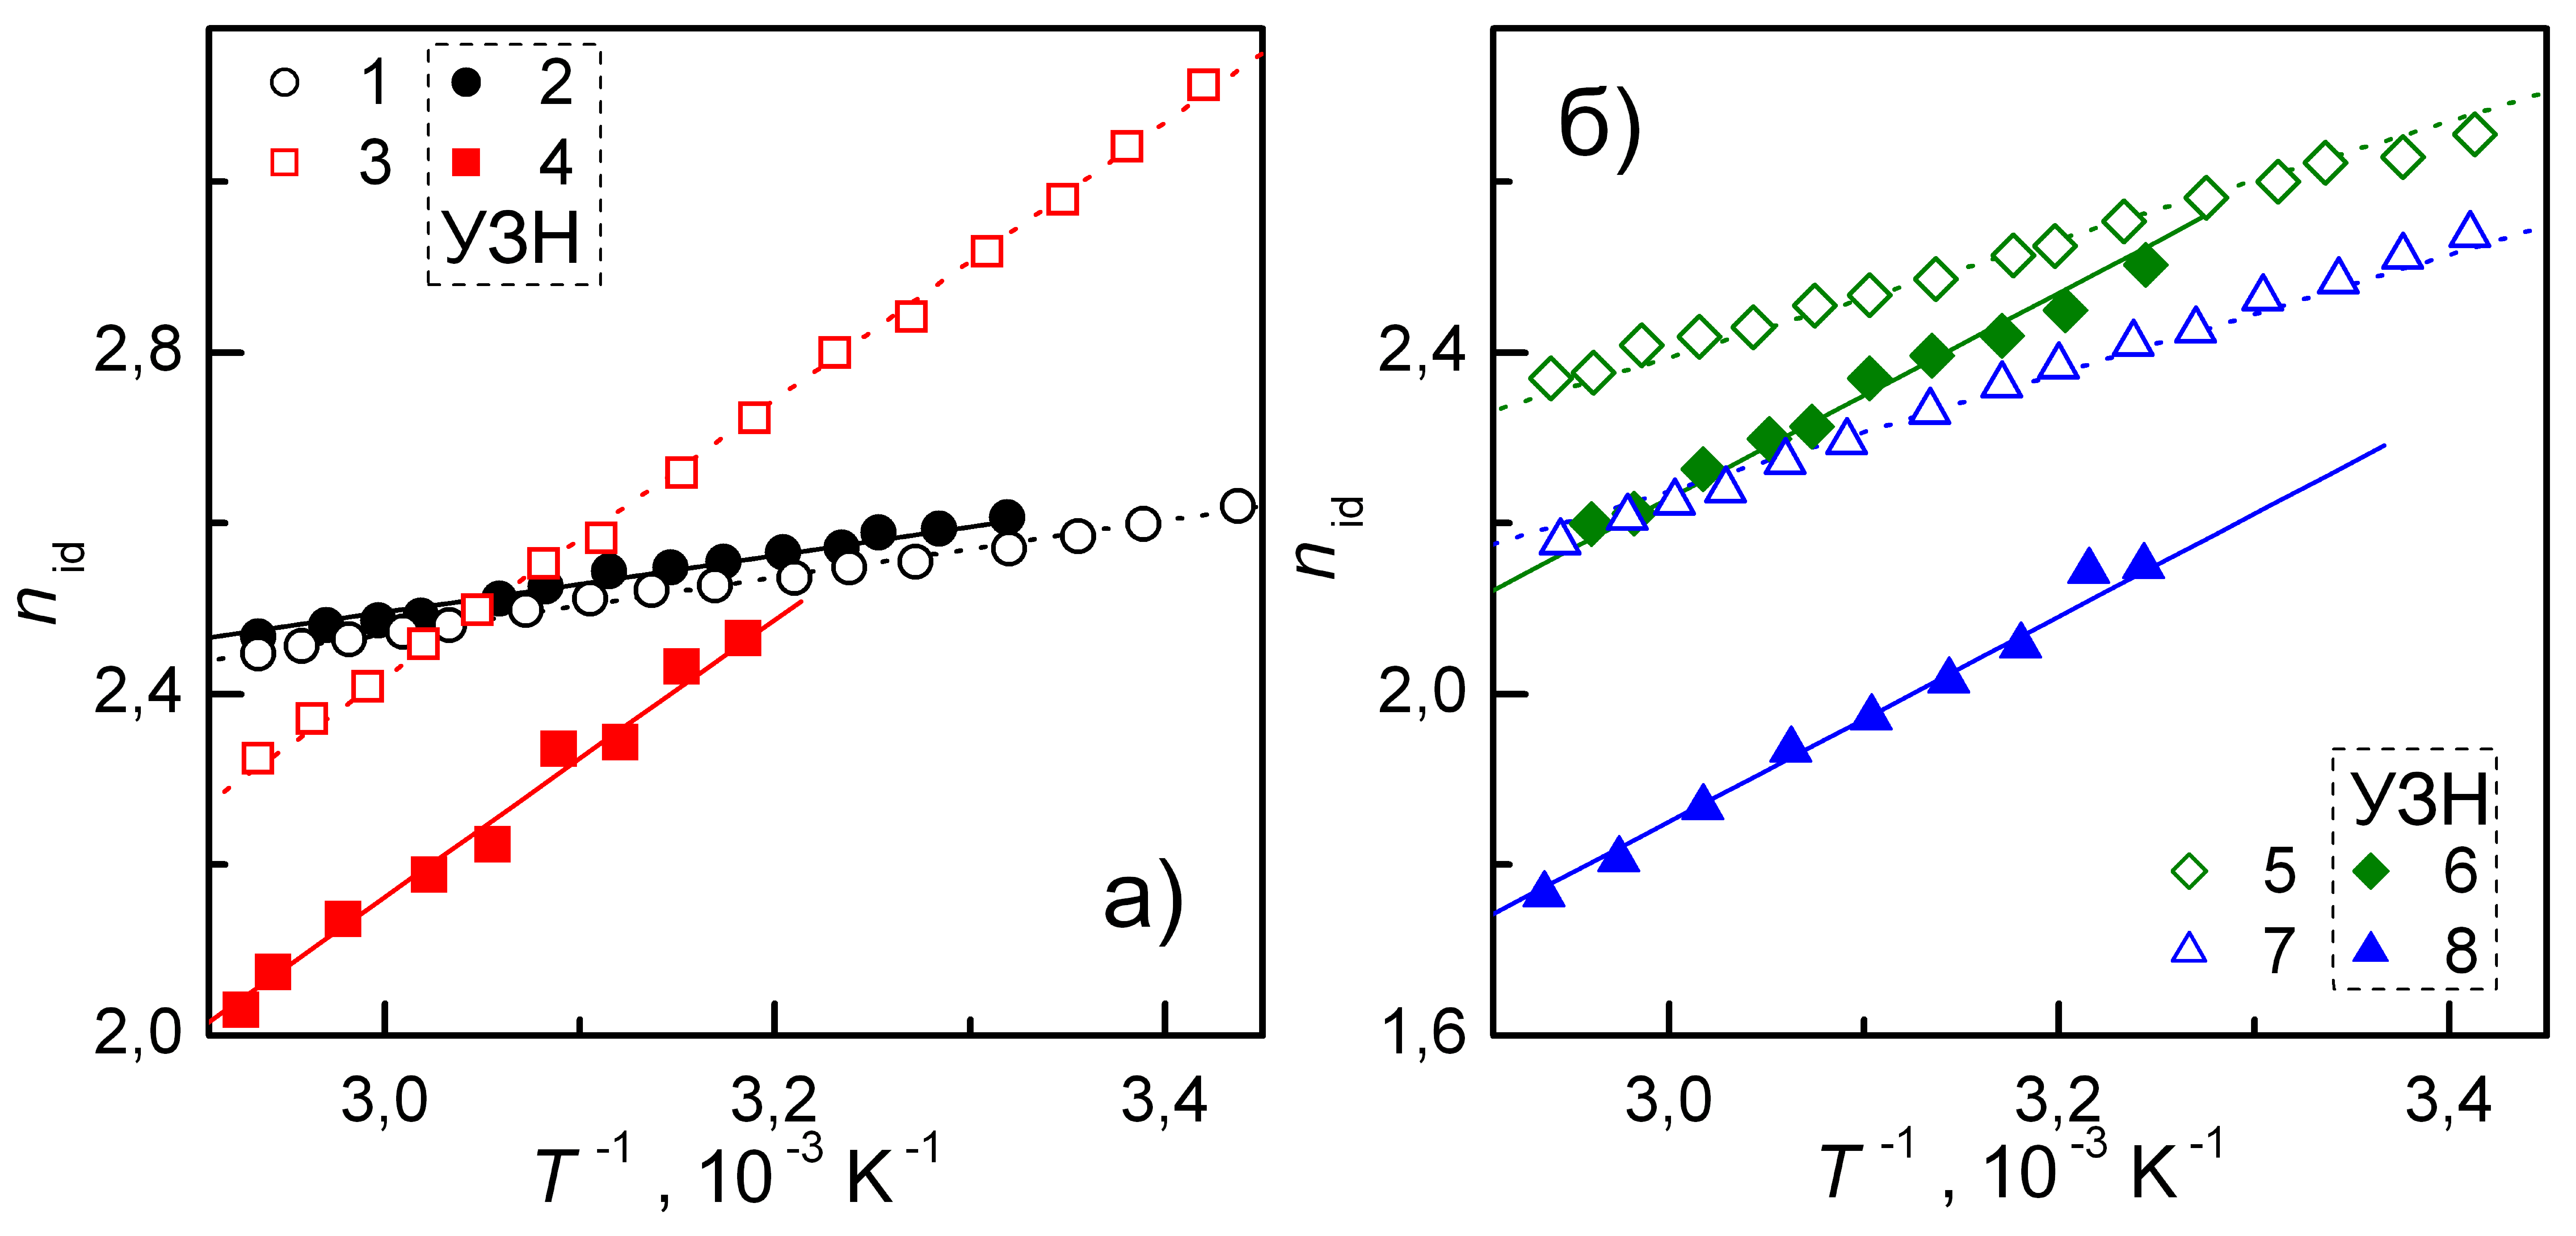
\includegraphics[width=0.95\textwidth]{fignRD}%
\caption{\label{fignRD}
Температурні залежності фактору неідеальності
\FigCaptionSSCRD
Точки --- експеримент,
лінії -- результат апроксимації з використанням формули~(\ref{eq_nT}).
}%
\end{figure}


\begin{figure}
\center
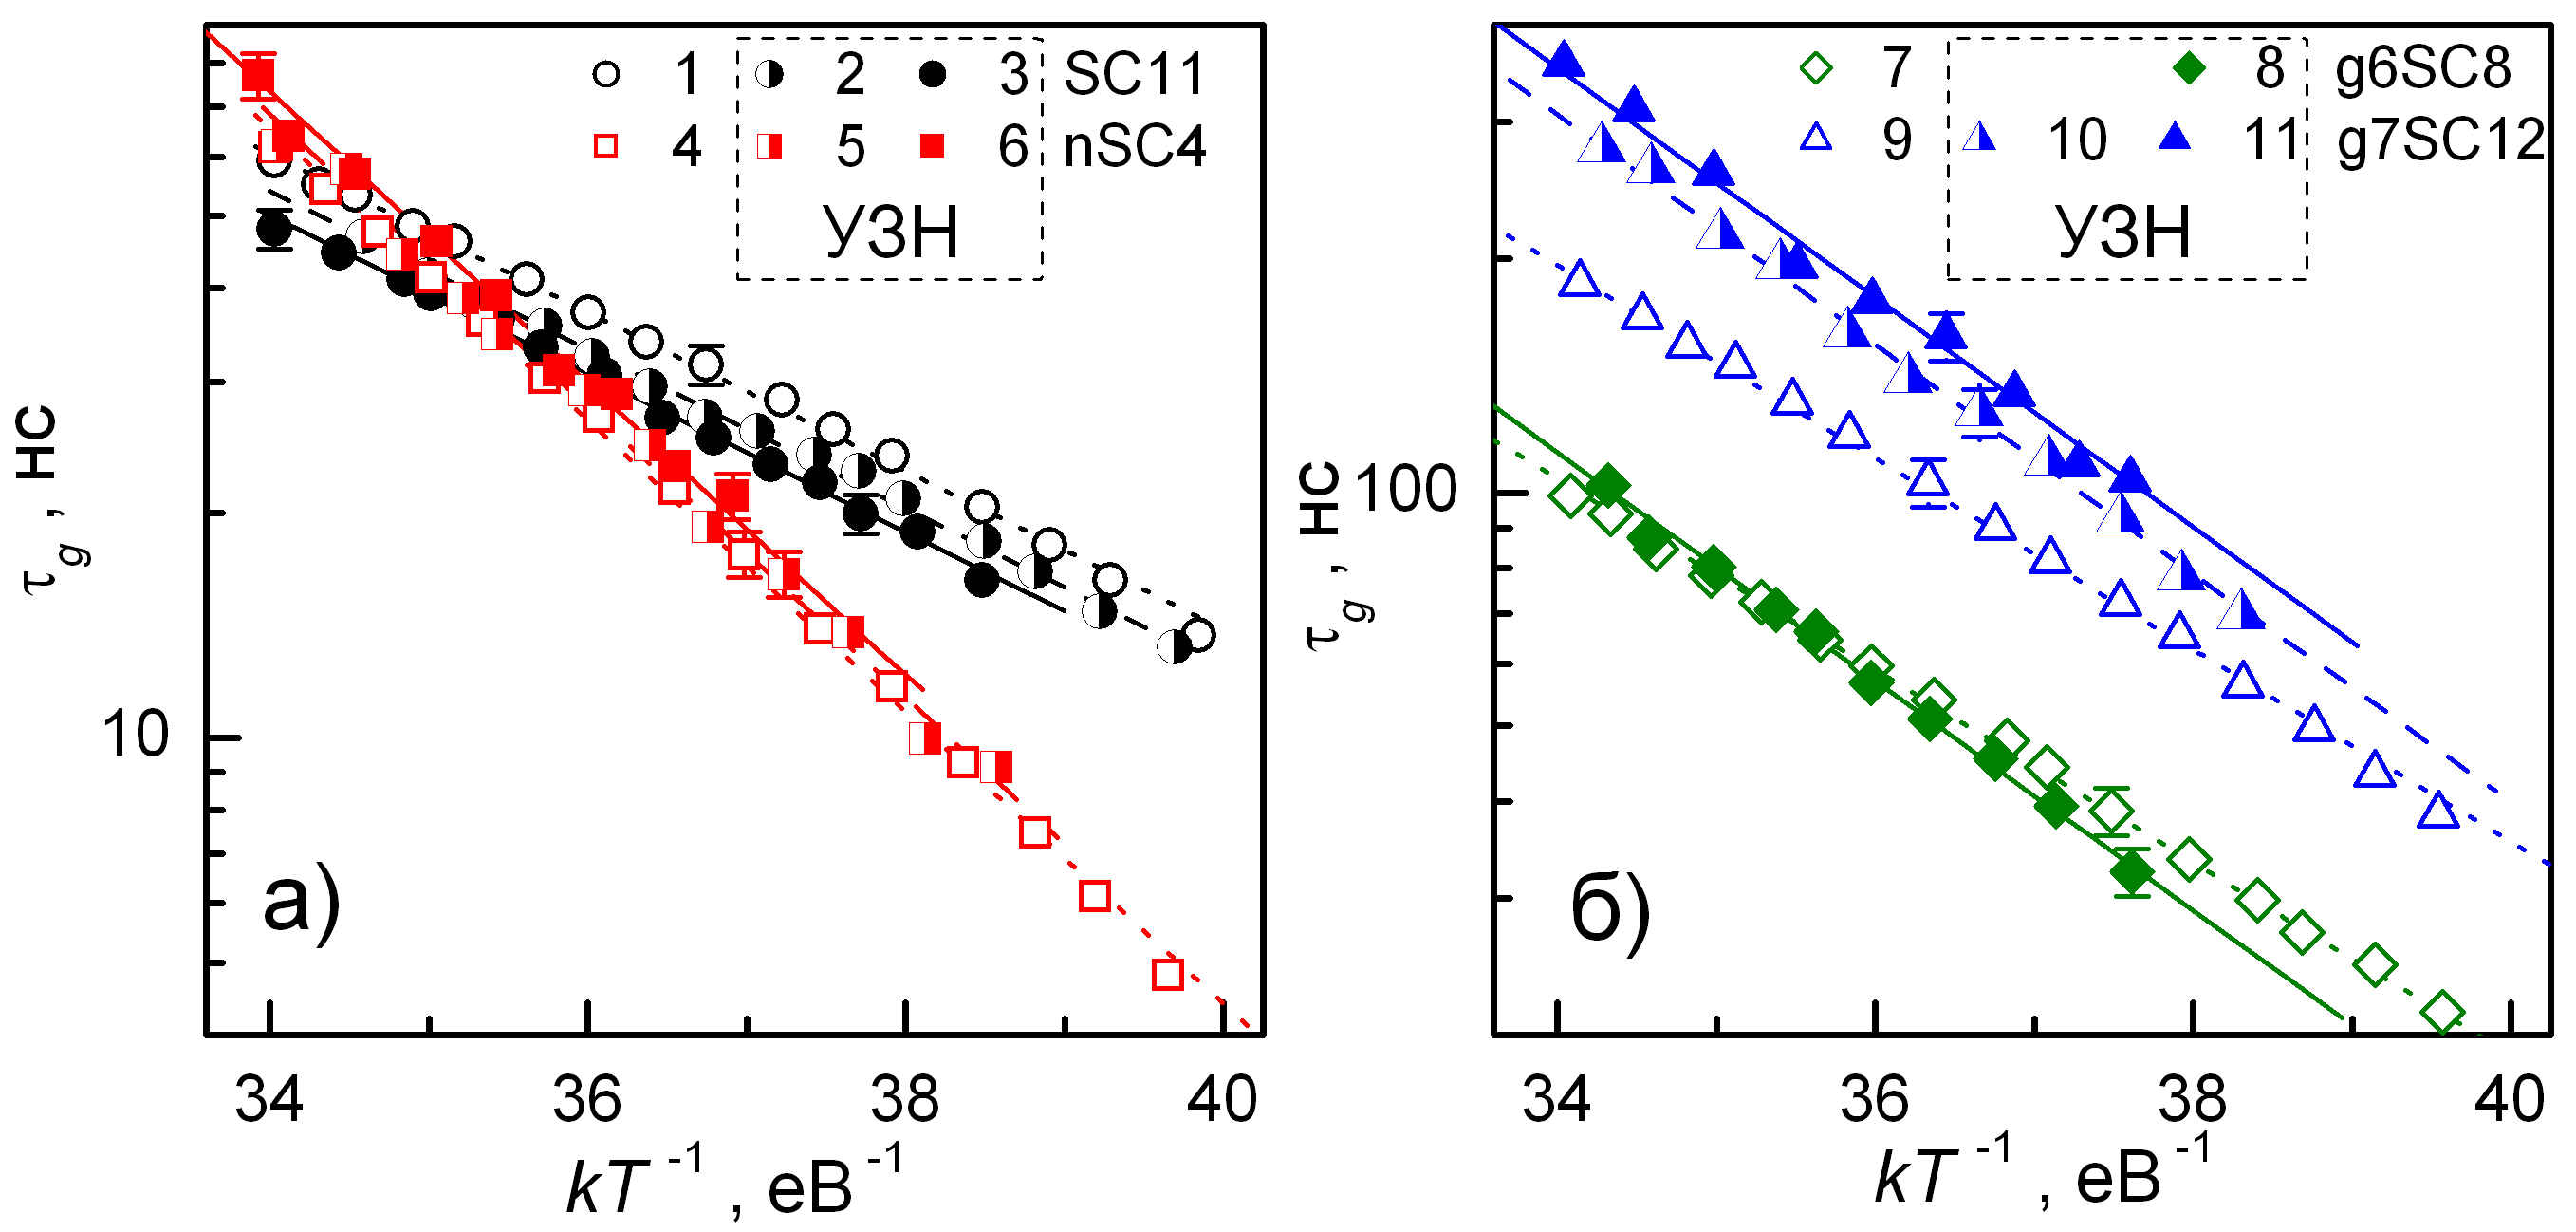
\includegraphics[width=0.95\textwidth]{figTAUgRD}%
\caption{\label{figTAUgRD}
Температурні залежності часу життя в ОПЗ.
Позначення кривих збігаються з Рис.~\ref{fignRD}.
%\FigCaptionSSCRD
Точки --- експеримент,
лінії -- результат апроксимації з використанням формули~(\ref{eq_TAUgT}).
}%
\end{figure}

З рисунків видно, що фактор неідеальності у опромінених структурах зі зменшенням температури зростає,
тоді як для $\tau_{g}$ спостерігається зворотна залежність.
Загалом, зміни $n_{\mathrm{id}}$ та $\tau_{g}$ з температурою добре описуються, як і для неопромінених зразків (див. параграф~\ref{sbQNR}),
 формулами (\ref{eq_nT}) та
(\ref{eq_TAUgT}), відповідно.
Результати відповідної апроксимації також наведені на Рис.~\ref{fignRD} та Fig.~\ref{figTAUgRD},
а визначені значення $T_{\mathrm{id}}$ and $E_{\tau g}$ --- в Таблиці~\ref{tabSSCparRD}.

\begin{table}
\caption{\label{tabSSCparRD}Характеристичні величини температурних залежностей параметрів опромінених та неопромінених
структур $n^+$--$p$--Si.
}
\begin{tabular}{|c|c|c|c|c|c|} \hline
Зразок&УЗН&$T_{\mathrm{id}}$, K&$E_{\tau g}$, еВ&$R_{293,\mathtt{Al}}$, кОм&$\sigma_{\mathtt{dis}}$, $10^4$~K/Ом\\
\hline
SC11&нема&$330\pm30$&$0.24\pm0.01$&$27\pm3$&$41\pm4$\\ \hline
&U--Ts2&$310\pm30$&$0.24\pm0.01$&$27\pm3$&$50\pm4$\\ \hline
&U--Tb3&$360\pm30$&$0.24\pm0.01$&$26\pm3$&$58\pm4$\\ \hline
nSC4&нема&$1610\pm70$&$0.45\pm0.02$&$2.2\pm0.4$&$65\pm7$\\ \hline
&U--Ts3&$1600\pm70$&$0.44\pm0.02$&$2.3\pm0.4$&$95\pm10$\\ \hline
&U--Tb3&$1680\pm70$&$0.44\pm0.02$&$2.2\pm0.4$&$130\pm10$\\ \hline
g6SC8&нема&$610\pm40$&$0.28\pm0.01$&$0.7\pm0.1$&$19\pm2$\\ \hline
&U--Tb2&$1080\pm50$&$0.33\pm0.02$&$0.8\pm0.1$&$24\pm2$\\ \hline
g7SC12&нема&$770\pm50$&$0.29\pm0.01$&$0.41\pm0.06$&$26\pm3$\\ \hline
&U--Ts1&$1260\pm60$&$0.34\pm0.02$&$0.39\pm0.06$&$45\pm4$\\ \hline
&U--Tb1&$1270\pm60$&$0.35\pm0.02$&$0.38\pm0.06$&$55\pm4$\\ \hline
\end{tabular}
\end{table}

При аналізі отриманих результатів, хотілося б наголосити на наступних виявлених особливостях:
\begin{enumerate}[label=\asbuk*),leftmargin=0em,itemindent=1.5em]
\item опромінення викликає зміну величин  $T_{\mathrm{id}}$ та $E_{\tau g}$, причому
 для  g6SC8 характеристична температура фактора неідеальності та характеристична енергія часу життя в ОПЗ
 близькі, за схожих умов, до відповідних значень  g7SC12;

\item в умовах УЗН спостерігається, як і для неопромінених структур, модифікація величин $n_{\mathrm{id}}$ та $\tau_g$;
  величини відповідних змін наведено в Таблиці~\ref{tabAIchangeRD};

\item $\Delta n_{\mathrm{id}}$ та $\varepsilon_{\tau g}$ змінюються при збільшенні $W_{\mathtt{US}}$,
 тоді як $T_{\mathrm{id}}$ та $E_{\tau g}$ практично не залежать від інтенсивності УЗН;

\item УЗН викликає збільшення як  $T_{\mathrm{id}}$, так і $E_{\tau g}$ в $\gamma$--опромінених структурах
(див. Рис.~\ref{fignRD},б та Рис.~\ref{figTAUgRD},б),
тоді як подібний ефект не спостерігається в неопромінених та нейтронно--опромінених зразках
(див. Рис.~\ref{fignRD},а та Рис.~\ref{figTAUgRD},а);

\item АІ зміни фактору неідеальності та часу життя в ОПЗ в опромінених та неопромінених зразках мають протилежний знак
 (для g6SC8 не у всьому температурному діапазоні);

\item зміни фактору неідеальності в умовах УЗН значно більші в радіаційно--модифікованих структурах.
\end{enumerate}


\begin{table}
\caption{\label{tabAIchangeRD}Акусто--індуковані зміни параметрів структур $n^+$-$p$--Si (при 330~K).
}
\center
\begin{tabular}{|c|c|c|c|c|c|} \hline
Зразок&УЗН&$\Delta n_{\mathrm{id}}$, $\pm0.01$&$\varepsilon_{\tau g}$, $\pm5$\%&$\varepsilon_{1/\tau n}$, $\pm0.2$&$\varepsilon_{\sigma\mathtt{dis}}$, $\pm10$\%\\
%&&\mbox{($\pm0.01$)}&($\pm5$\%)&($\pm0.2$)&($\pm10$\%)\\
\hline
SC11&U--Ts2&$-0.02$&14&0.7&$-20$\\
&U--Tb3&$-0.03$&17&1.4&$-40$\\ \hline
nSC4&U--Ts3&0.13&$-5$&1.5&$-50$\\
&U--Tb3&0.26&$-13$&3.0&$-100$\\ \hline
g6SC6&U--Tb2&0.15&$-2$&2.3&$-30$\\ \hline
g7SC12&U--Ts1&0.26&$-49$&0.9&$-70$\\
&U--Tb12&0.36&$-70$&1.9&$-110$\\ \hline
\end{tabular}
\end{table}

Особливості рекомбінації в ОПЗ (великі значення $n_\mathrm{id}$, малі величини та температурна залежність $\tau_g$)
однакові, як  для опромінених структур так і неопромінених.
Тому доцільно припустити, що для nSC4, g6SC8 та g7SC12 процеси в області просторового заряду також можна описати
за допомогою моделі рекомбінації у системі спарених рівнів дефектів, яка детально описана в параграфі~\ref{sbQNR}.
Для пояснені АІ змін параметрів також доцільно залучити модель акусто--активного комплексного дефекту - див. параграф~\ref{sbAEDefect}.
А отже, враховуючи експериментально отримані результати та оцінки, отримані на основі моделі,
\begin{enumerate}[label=\asbuk*),leftmargin=0em,itemindent=1.5em]
\item так як $E_{\tau g}$ (особливо) та $T_{\mathrm{id}}$ (менше) визначаються положенням рівнів, зв'язаних
зі спареними дефектами, то їх зміна в nSC4, g6SC8 та g7SC12 порівняно з SC11 свідчить про те, що
після опромінення змінилися дефекти (або донор, або акцептор, або й обидва), які приймають участь у CDLR;
при цьому за рекомбінацію в g6SC8 та g7SC12 відповідають однакові за типом дефекти (проте з різною концентрацією,
 так як $T_{\mathrm{id}}$ збігаються не абсолютно), які відрізняються від рекомбінаційно активних дефектів в ОПЗ нейтронно--опроміненого зразка;

\item  АІ зміни   $E_{\tau g}$ (та $T_{\mathrm{id}}$), які спостерігаються лише в g6SC8 and g7SC12,
 свідчать про перебудову РД, створених внаслідок $\gamma$--опромінення;
 так як зміни оборотні, то йде мова про те, що відповідні
 гамма--індуковані РД є конфігураційно бістабільними (або метастабільними) і під дією УЗ відбувається їх перебудова з основного стану,
 властивого ненавантаженій внаслідок поширення пружних коливань ґратці;
 подібні АІ перетворення дефектів спостерігалися і раніше \cite{Wosinski,Ostapenko1994,YOlikhTPL2011r};

 \item знак АІ $\varepsilon_{\sigma}$ не міняється (див. Рис.~\ref{figR2L},а та формулу~(\ref{eqEpsSig})), тоді як
  знак  $\varepsilon_{\mathtt{RDA}}$  може мінятися для пари, що складається з дефектів, яким відповідають протилежні
  змінами об'єму кристалу (див. Рис.~\ref{fig_Erda});
  отже зміна знаків $\Delta n_{\mathrm{id}}$ та $\varepsilon_{\tau g}$ свідчить про перехід від випадку
  $(\Delta\Omega_d^\mathtt{D}\cdot\Delta\Omega_d^\mathtt{A}>0)$ до
  $(\Delta\Omega_d^\mathtt{D}\cdot\Delta\Omega_d^\mathtt{A}<0)$ після опромінення;
  на користь такого переходу свідчить і підсилення ефективності впливу УЗН на дефекти в опромінених структурах.
\end{enumerate}

До речі, висновок зроблений в параграфі~\ref{sbDefectType} про те, що
в неопромінених структурах процеси CDLR проходять за участю кисневих преципітатів та комплексу Fe$_i$B$_s$ свідчить на користь
останнього твердження, так як обидва ці дефекти характеризуються $\Delta\Omega_d>0$, тобто є дефектами міжвузольного типу.
Таким чином, в опромінених структурах один з компонентів CDLR--пари
має мати вакансійний тип ($\Delta\Omega_d<0$).

Щодо nSC4, то дефектом, який здатен пояснити АІ зміни $\tau_g$ та $n_\mathrm{id}$, цілком може бути дивакансія,
значна кількість яких утворюється при нейтронному опроміненні.
Проте у гамма--опромінених зразках очікується поява бістабільного (або метастабільного) дефекту.
Загалом у кремнії відомо лише декілька подібних дефектів з $\Delta\Omega_d<0$, а саме
\begin{itemize}
  \item VO$_2$ \cite{FTP:Murin},
  \item V$_3$ \cite{V3:Markevich},
  \item VO$_i$ \cite{MetaUFN}.
\end{itemize}
Проте комплекс VO$_2$ утворюється в радіаційно--опромінених кристалах після відпали при $300^\circ$C,
V$_3$ не є типовим дефектом для кремнію, опроміненого $\gamma-^{60}$Co,
тоді як VO$_i$ при цьому утворюються у достатній кількості (див. Таблицю~\ref{tabDefectNt}) і можуть приймати
участь в CDLR в околі $n^+$--$p$ інтерфейсу в g6SC8 and g7SC12.
Метастабільний стан VO$_i$ зазвичай спостерігається при низьких температурах
і відрізняється більшою відстанню між вакансією та киснем та глибшим розташуванням енергетичного рівня \cite{MetaUFN}.
Для комплексу як цілого $\Delta\Omega_d(\mbox{VO}_i)<0$,
проте для його компонент $\Delta\Omega_d(\mbox{V})<0$ та $\Delta\Omega_d(\mbox{O}_i)>0$.
Таким чином, згідно зі зробленими при розгляді акусто--активного комплексу припущеннями,
VO$_i$ є цілком придатним для АІ зміни відстані між компонентами.
Отримані результати свідчать, що під дією УЗН  відбувається
перехід VO$_i$ у метастабільну конфігурацію, що, в свою чергу,
викликає зміни $T_{\mathrm{id}}$ та $E_{\tau g}$.





\subsection{Квазі--нейтральна область\label{sbRadDef}}

Чисельним показником рекомбінаційних процесів, які відбуваються в КНО $p$-$n$ структури є
час життя неосновних носіїв заряду.
Рис.~\ref{figTAUrRD} відображає виявлену поведінку $\tau_n$ зі зміною температури як для опромінених зразків,
так і неопромінених, як при застосуванні УЗН, так і без нього.
Загалом, залежності $\tau_n$ від температури та УЗН не змінюються після радіаційного впливу.
Вихідні значення $\tau_n$ знаходяться в діапазоні $2\div5$~мкс для різних зразків,
що відповідає довжинам дифузії $80\div130$~мкм.
При опроміненні використовувалися не дуже високі дози і тому
такий розкид значень часів життя не зв'язаний саме з радіаційним впливом,
а швидше визначається неоднорідністю вихідної пластини, з якої були виготовлені зразки.
Подібна неоднорідність зустрічається досить часто \cite{Oxide:Chen,Oxide_Schon}.


\begin{figure}
\center
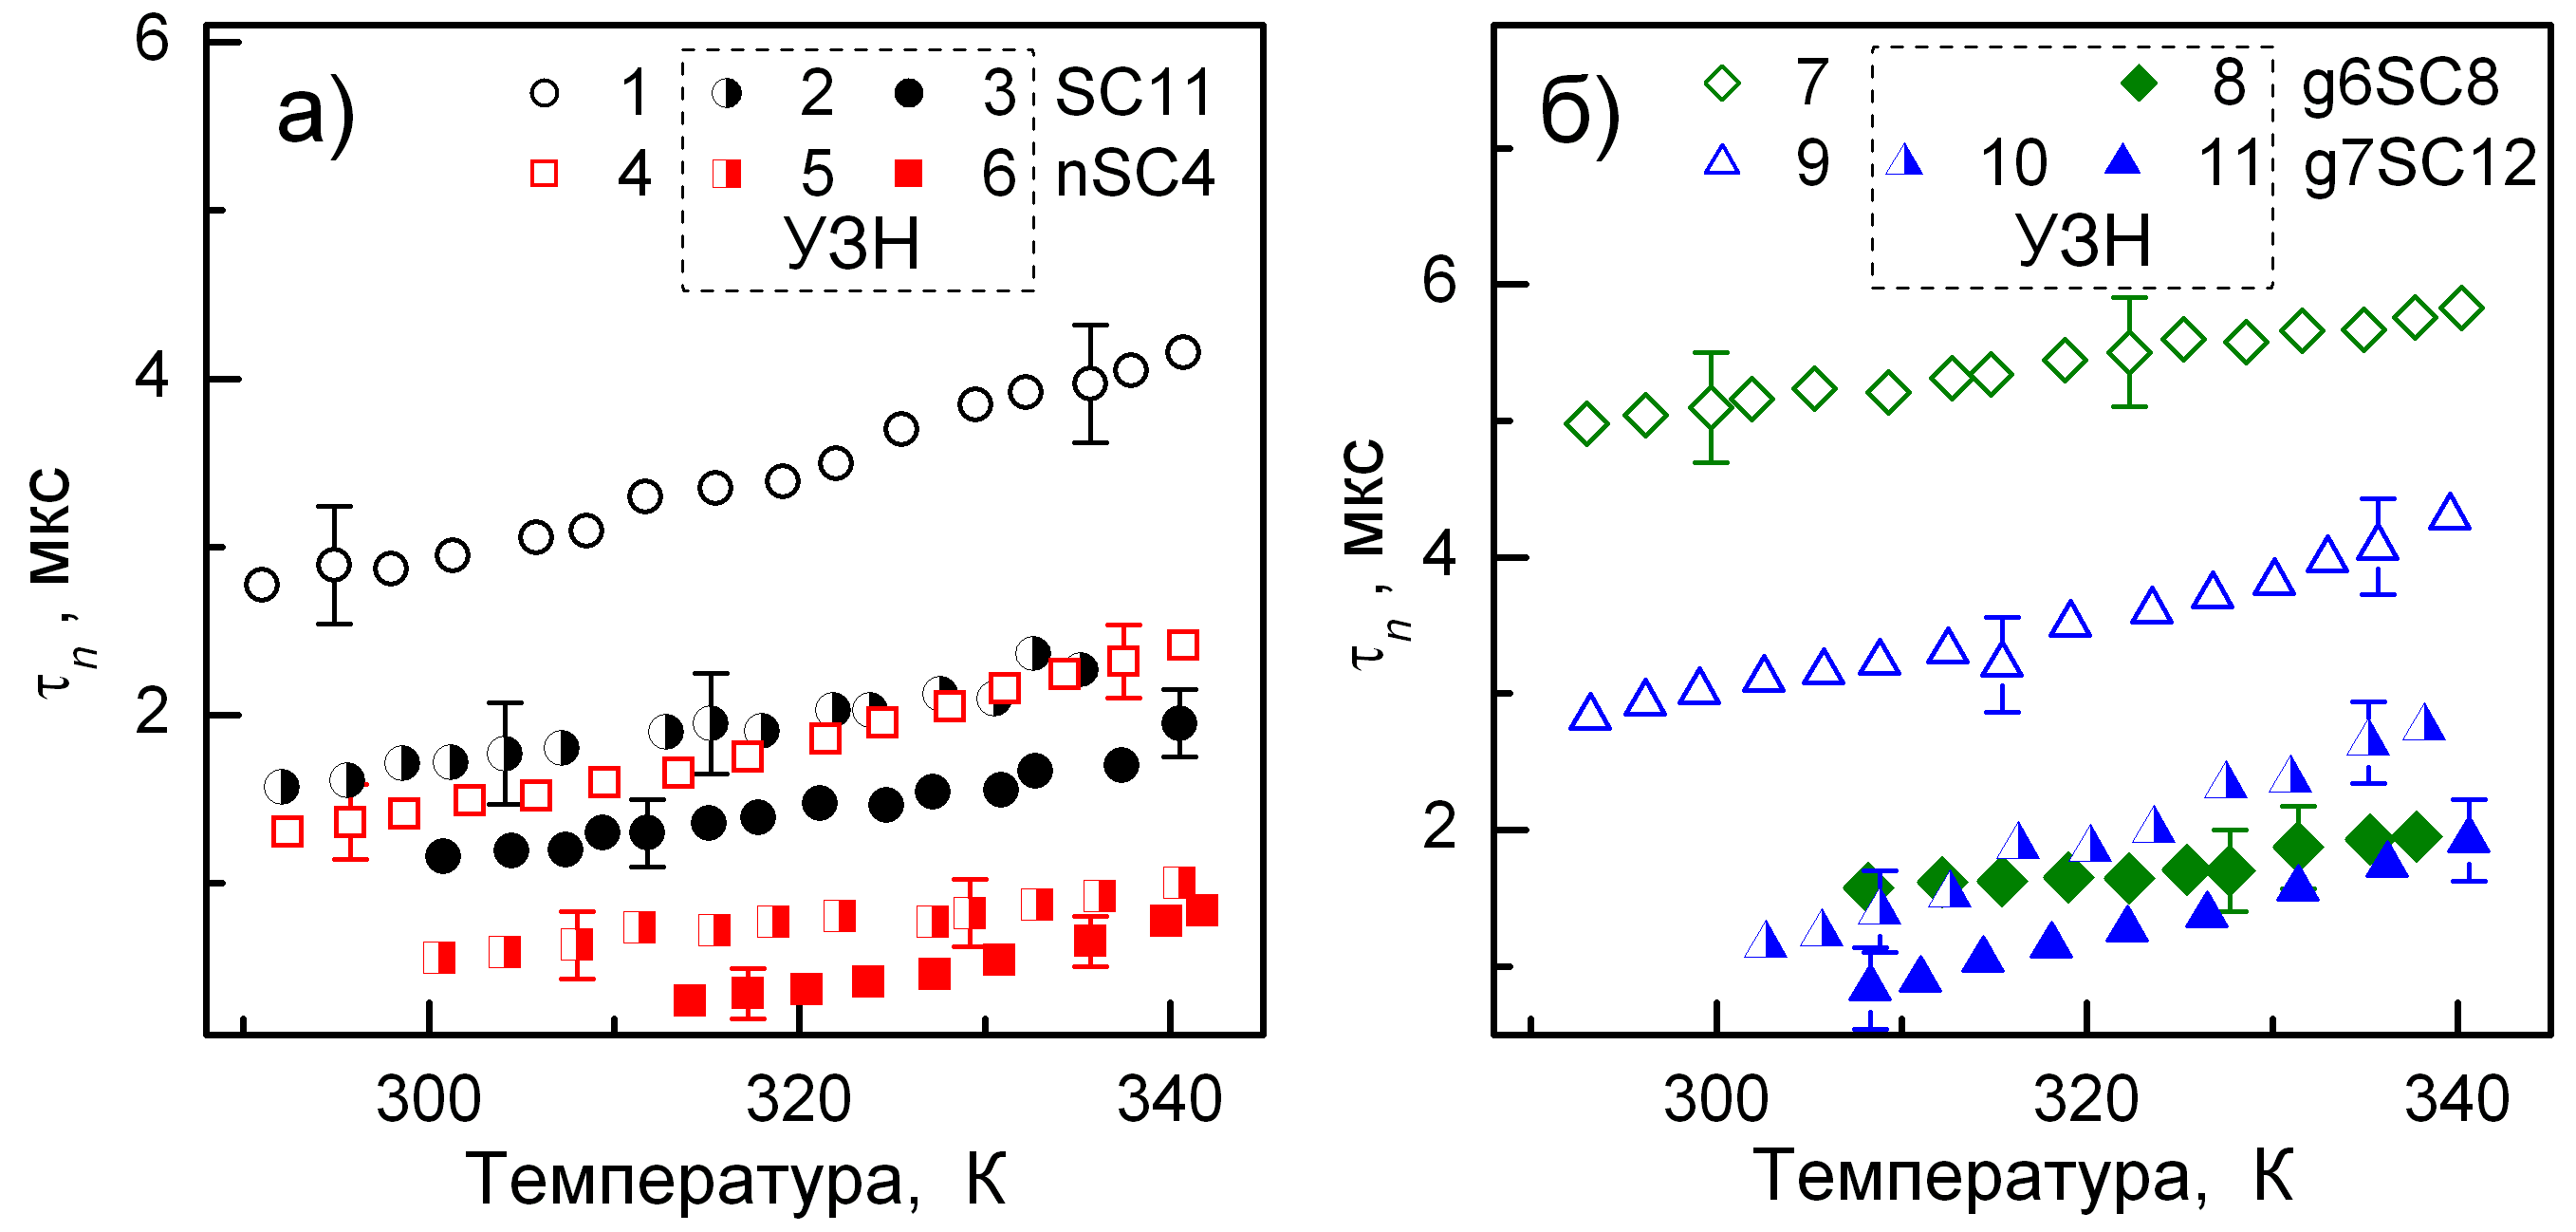
\includegraphics[width=0.95\textwidth]{figTAUrRD}
\caption{\label{figTAUrRD}
Температурні залежності часу життя неосновних носіїв заряду в КНО
\FigCaptionSSCRD
%. Позначення кривих збігаються з Рис.~\ref{fignRD}.
}%
\end{figure}

З іншого боку, для опису радіаційно--індукованого зменшення часу життя використовується формула Messenger–-Spratt \cite{Markvart}:
\begin{equation}
\label{eqMS}
\tau_n^{-1}=\tau_{n0}^{-1}+K_\tau\Psi\,,
\end{equation}
де
$\tau_{n0}$ відповідає неопроміненому зразку, а
$K_\tau$ --- константа пошкодження часу життя (lifetime damage constant).
Загалом $K_\tau$ залежить від кристалу, типу опромінення і насамперед визначається величиною NIEL.
Відомі з літератури значення $K_\tau$ для Cz--Si та проведені з використанням виразу (\ref{eqMS}) оцінки відповідних
змін оберненого часу життя наведено в Таблиці~\ref{tabTAUn}.
Як видно з наведених даних, оцінені значення радіаційно--індукованих змін $\tau_n^{-1}$ складають лише
(8-17), 4 та 29\% виміряних значень для зразків nSC4, g6SC8 та g7SC12, відповідно, а отже не можуть
пояснити екпериментально виявлений розкид даного параметру.

\begin{table}
\caption{\label{tabTAUn}Виміряні та оцінені параметри часу життя в КНО.
}
\center
\begin{tabular}{|c|c|c|c|c|}
\hline
Зразок &$\tau_{n,in}^{-1}$ (320~K), 10$^5$~с$^{-1}$&$K_\tau$, см$^2/$с&$K_\tau\times\Psi$, 10$^4$~с$^{-1}$&$K_\mathtt{US}^\mathtt{eff}$, см$^2/$Вт\\ \hline
SC11&2,9&$\ldots$&$\ldots$&3,5\\ \hline
\multirow{2}{*}{nSC4}&\multirow{2}{*}{4,7}&10$^{-7}$ \cite{NIEL:Jafari}&\multirow{2}{*}{4$\div$8}&\multirow{2}{*}{7,1}\\ %\hline
&&2$\times$10$^{-7}$ \cite{n:Gaubas}&&\\ \hline
g6SC8&1,8&5$\times$10$^{-12}$&0,8&6,0\\ \cline{1-2} \cline{4-5}%\hline
g7SC12&2,8& \cite{NIEL:Jafari,gamma:Kolkov} &8&5,2\\ \hline
\end{tabular}
\end{table}

З іншого боку,
оцінка впливу утворених РД на час життя неосновних носіїв заряду в КНО може бути проведена спираючись
на вираз (\ref{eqTAUSHRsum}).
При цьому необхідно взяти до уваги,
що VO$_i$ не є рекомбінаційно--активним центром у $p$--Si \cite{gamma:Kolkov,IrrCzpSi:Benton,IrrCzpSi:Coffa,IrrCzpSi:Ganagona,IrrCzpSi:Vines}.
Була проведена оцінка величин $\tau_{n,\mathtt{RD}}^{-1}$ (оберненого часу життя, пов'язаного з рекомбінацією на окремих РД)
для C$_i$O$_i$, V$_2$ та  V$_3$, спираючись на їх концентрацію (див. Таблицю~\ref{tabDefectNt}) та відомі з літератури значення ППЗ електронів.
Отримані результати наведено в Таблиці~\ref{tabDefectTAU}.
Видно, що на $\tau_n$ в гамма--опромінених зразках переважно впливають комплекси C$_i$O$_i$, тоді як для nSC4 основні очікувані
зміни часу життя пов'язані з вакансійними кластерами.
Зауважимо, що для nSC4, g6SC8 та g7SC12 сума величин $\tau_{n,\mathtt{RD}}^{-1}$ для різних дефектів
непогано збігається з відповідними значеннями $(K_\tau\cdot\Psi)$ (Таблиця~\ref{tabTAUn})




\begin{table}[b]
\caption{\label{tabDefectTAU}Оцінка впливу окремих РД на час життя неосновних носіїв в КНО.
}
\center
\begin{tabular}{|c|c|c|c|c|}
\hline
Дефект&$\sigma_n$,&\multicolumn{3}{c|}{$\tau_{n,\mathtt{RD}}^{-1}$, 10$^4$~с$^{-1}$}\\ \cline{3-5}
&10$^{-15}$~см$^2$&nSC&g6SC&g7SC\\
\hline
C$_i$O$_i$&0,7 \cite{gamma:Stahl}, 0,9 \cite{gamma:Kolkr}&0,8--1&0,9--1,1&9--11\\ \hline
V$_2$&3 \cite{gamma:Stahl}, 2 \cite{A:Brothe}&2,2--3,3&0,1--0,2&1--2\\ \hline
V$_3$&2,4 \cite{V3:Markevich}&0,7&---&---\\ \hline
\end{tabular}
\end{table}

Рис.~\ref{figTAUrRD} показує, що УЗН викликає зменшення $\tau_n$.
З виразу (\ref{eqTAUSHRsum}) видно, що при аналізі змін $\tau_n$
зручніше розглядати відносні зміни оберненого часу життя
\begin{equation*}
  \varepsilon_{1/\tau n}=\frac{\tau_{n,\mathtt{US}}^{-1}-\tau_{n,in}^{-1}}{\tau_{n,in}^{-1}}=\frac{\tau_{n,in}-\tau_{n,\mathtt{US}}}{\tau_{n,\mathtt{US}}}\,.
\end{equation*}
АІ значення наведено в Таблиці~\ref{tabAIchangeRD}.

Використовуючи модель акусто--активного комплексу (параграф~\ref{sbAEDefect}, формули (\ref{eqEpsSigUS}) та (\ref{eqEpsSigUSA}))
вираз для $\varepsilon_{\tau n}$ можна перетворити наступним чином
\begin{equation}
\label{eqEpsTAU}
\varepsilon_{1/\tau n}=K_\mathtt{US}^\mathtt{eff}W_\mathtt{US}\,,
\end{equation}
де
$K_\mathtt{US}^\mathtt{eff}$ характеризує АДВ у зразку і залежить від
концетрацій як ААД, так і не акусто--активних (non--AA) центрів
\begin{equation}
\label{eqKeff}
K_\mathtt{US}^\mathtt{eff}=\sum_j^{M_d^\mathtt{AA}}\frac{\tau_{n,in}}{\tau_{n,j,in}}K_\mathtt{US,j}^{*}\,.
\end{equation}
Як вже було зазначено, $K_\mathtt{US,j}^*$ описує взаємодію $j$--го рекомбінаційного центру з ультразвуком.
Отримані залежності $\varepsilon_{1/\tau n}$ від $W_\mathtt{US}$ показано на Рис.~\ref{figKusRD}.
Лінійність цих залежностей ще раз підтверджує справедливість припущень, використаних при побудові
моделі.
Визначені величини $K_\mathtt{US}^\mathtt{eff}$ наведено в Таблиці~\ref{tabTAUn}.


\begin{figure}
\center
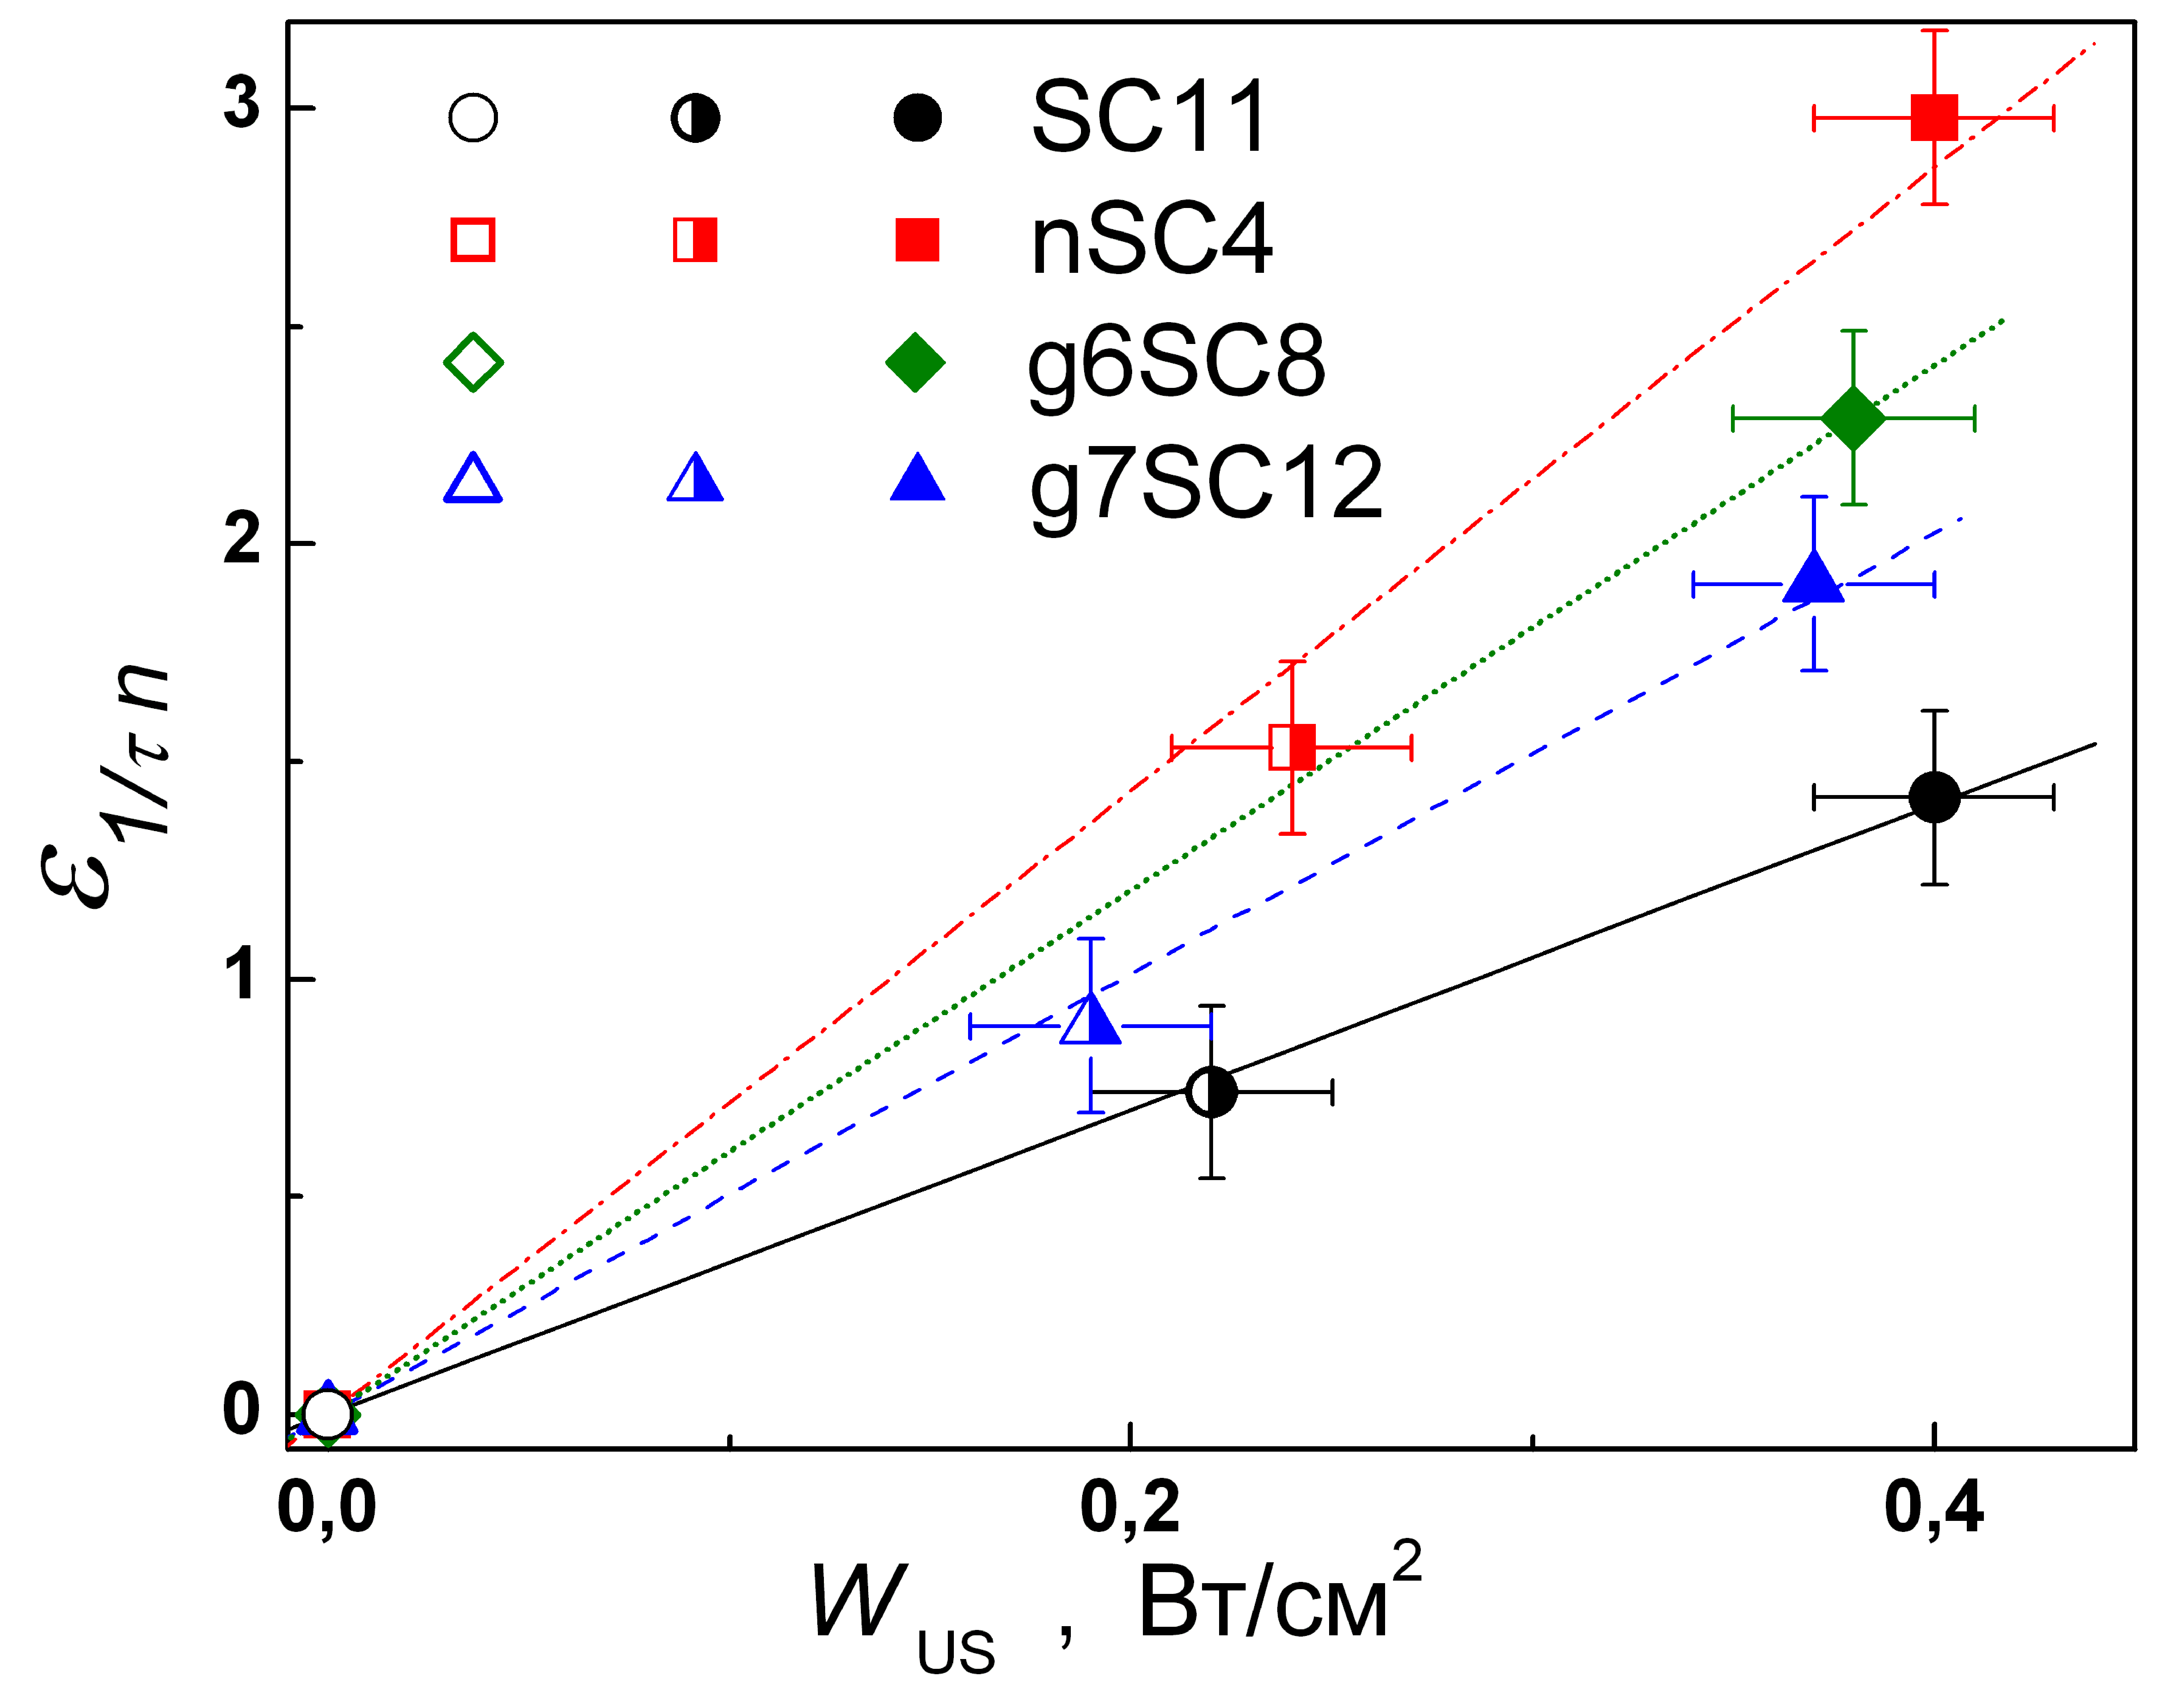
\includegraphics[width=0.65\textwidth]{figKusRD}
\caption{\label{figKusRD}
Залежності відносних змін оберненого часу життя в ОПЗ від інтенсивності УЗ для
неопроміненого (кола), нейтронно--опроміненого (квадрати) та $\gamma$--опромінених (трикутники та ромби) зразків.
Лінії --- апроксимація згідно з формулою ~(\ref{eqEpsTAU}).
}%
\end{figure}

Припустимо,
що в неопромінених зразках присутні ААД лише одного типу, тобто $M_d^\mathtt{AA}=1$.
Відповідно до результатів, наведених в параграфі~\ref{sbDefectType}, це можуть бути дефекти, пов'язані з кисневмісними преципітатами.
Позначимо константи взаємодії УЗ із C$_i$O$_i$ та V$_n$ як $K_\mathtt{US}^\mathtt{CO}$ та $K_\mathtt{US}^\mathtt{V}$, відповідно.
В цьому випадку вираз для $K_\mathtt{US}^\mathtt{eff}$ в неопромінених та опромінених зразках
матиме вигляд (\ref{eqeqKeffInit}) та (\ref{eqeqKeffRD}), відповідно:
\begin{eqnarray}
K_\mathtt{US}^\mathtt{eff}&=&K_\mathtt{US}^\mathtt{AA}\,\tau_{n,in}/\tau_{n,in}^\mathtt{AA}\,,\label{eqeqKeffInit}\\
K_\mathtt{US}^\mathtt{eff}&=&K_\mathtt{US}^\mathtt{AA}\tau_{n,in}/\tau_{n,in}^\mathtt{AA}+
                           K_\mathtt{US}^\mathtt{CO}\tau_{n,in}/\tau_{n,\mathtt{RD}}^\mathtt{CO}+
                           K_\mathtt{US}^\mathtt{V}\tau_{n,in}/\tau_{n,\mathtt{RD}}^\mathtt{V} \,.\label{eqeqKeffRD}
\end{eqnarray}
У цих виразах $\tau_{n,in}^\mathtt{AA}$ --- час життя неосновних носіїв за умови, що рекомбінація
відбувається лише за участю ААД (non--AA рекомбінаційні центри відсутні),
а $K_\mathtt{US}^\mathtt{AA}$ описує АДВ з цим дефектом.

Для аналізу найбільш придатні два граничні випадки.
В першому з них вважається,
що ААД розподілені однорідно по кремнієвій пластині, тоді як
non--AA рекомбінаційні центри --- неоднорідно.
Іншими словами,
значення $\tau_{n,in}^\mathtt{AA}$ для зразків SC11, nSC4, g6SC8 та g7SC12
однакове, тоді як різниця величин
$(\tau_{n,in}^{-1}-K_\tau\cdot\Psi)$ визначається non--AA дефектами.
Використовуючи вирази (\ref{eqeqKeffInit}) та (\ref{eqeqKeffRD}) а також
дані таблиць \ref{tabTAUn} та \ref{tabDefectTAU}
була отримана наступна система рівнянь
\begin{eqnarray}
\mbox{SC11}:\,\,3.5&=&K_\mathtt{US}^\mathtt{AA}\cdot(\tau_{n,in}^\mathtt{AA})^{-1}\,/2.9\,,\nonumber\\
\mbox{nSC4}:\,\,7.1&=&K_\mathtt{US}^\mathtt{AA}\cdot(\tau_{n,in}^\mathtt{AA})^{-1}\,/4.7+0.09\,K_\mathtt{US}^\mathtt{V}+0.02\,K_\mathtt{US}^\mathtt{CO}\,,\nonumber\\
\mbox{g6SC8}:\,\,6.0&=&K_\mathtt{US}^\mathtt{AA}\cdot(\tau_{n,in}^\mathtt{AA})^{-1}\,/1.8+0.01\,K_\mathtt{US}^\mathtt{V}+0.05\,K_\mathtt{US}^\mathtt{CO}\,,\nonumber\\
\mbox{g7SC12}:\,\,5.2&=&K_\mathtt{US}^\mathtt{AA}\cdot(\tau_{n,in}^\mathtt{AA})^{-1}\,/2.8+0.05\,K_\mathtt{US}^\mathtt{V}+0.35\,K_\mathtt{US}^\mathtt{CO}\,,\nonumber
\end{eqnarray}
де
$(\tau_{n,in}^\mathtt{AA})^{-1}$ вимірюється в $10^4$~с$^{-1}$.
Ці рівняння є справедливими за умови, що
$K_\mathtt{US}^\mathtt{AA}\cdot(\tau_{n,in}^\mathtt{AA})^{-1}=(10\pm3)$~см$^2$~Вт$^{-1}$,
$K_\mathtt{US}^\mathtt{V}=(42\pm15)$~см$^2$~Вт$^{-1}$,
$K_\mathtt{US}^\mathtt{CO}=0$.
Так як  $(\tau_{n,in}^\mathtt{AA})^{-1}<1,83$,
то $K_\mathtt{US}^\mathtt{AA}>5$~см$^2$~Вт$^{-1}$.

У іншому граничному випадку вважається,
що non--AA розподілені по пластині рівномірно,
тоді як ААД визначають відмінність значень $(\tau_{n,in}^{-1}-K_\tau\cdot\Psi)$ у різних зразках.
Проте, якщо записати систему рівнянь, використовуючи дані припущення,
то виявляється що експериментально визначені значення $K_\mathtt{US}^\mathtt{eff}$
приводять до фізично неправильних (від'ємних) значень $K_\mathtt{US,j}^*$.
Подібні нереальні результати отримуються і у припущені, що $M_d^\mathtt{nonAA}=0$
(non--AA рекомбінаційні центри відсутні).

Таким чином, отримані результати дозволяють зробити висновок,
що лише частина дефектів, пов'язаних з КП, є акусто--активними.
Вони розподілені достатньо рівномірно по вихідній кремнієвій пластині і саме їх модифікація
в умовах УЗН є причиною виявлених зміни часу життя неосновних носіїв заряду в неопромінених та $\gamma$--опромінених зразках.
Ефект АІ зміни $\tau_n$ підсилюється внаслідок АІ модифікації дивакансій у нейтронно--опромінених структурах.
Іншими словами,
C$_i$O$_i$ не є акусто--активним дефектом, тоді як V$_2$ має подібні властивості.



\subsection{Акусто--індуковані зміни шунтуючого опору\label{sbRsh}}

На Рис.~\ref{figRshRD} наведено залежність величини шунтуючого опору опромінених та неопромінених структур
за умов УЗН та без нього для дослідженого температурного інтервалу.
Як видно з рисунку, опромінення викликає достатньо суттєве зниження шунтуючого опору, а отже
і збільшення шунтуючого струму.
Крім того, після $\gamma$--опромінення відбувається зміна температурної залежності $R_{sh}$:
так, якщо для SC11 та nSC4 спостерігається зменшення шунтуючого опору з ростом температури,
то для g6SC8 та g7SC12 в околі 293~K спостерігається майже лінійне збільшення залежності
$R_{sh}$ від $T$.
Зауважимо, що вісь $R_{sh}$ на Рис.~\ref{figRshRD},a має логарифмічний масштаб і лінійний на  Рис.~\ref{figRshRD},б.


\begin{figure}
\center
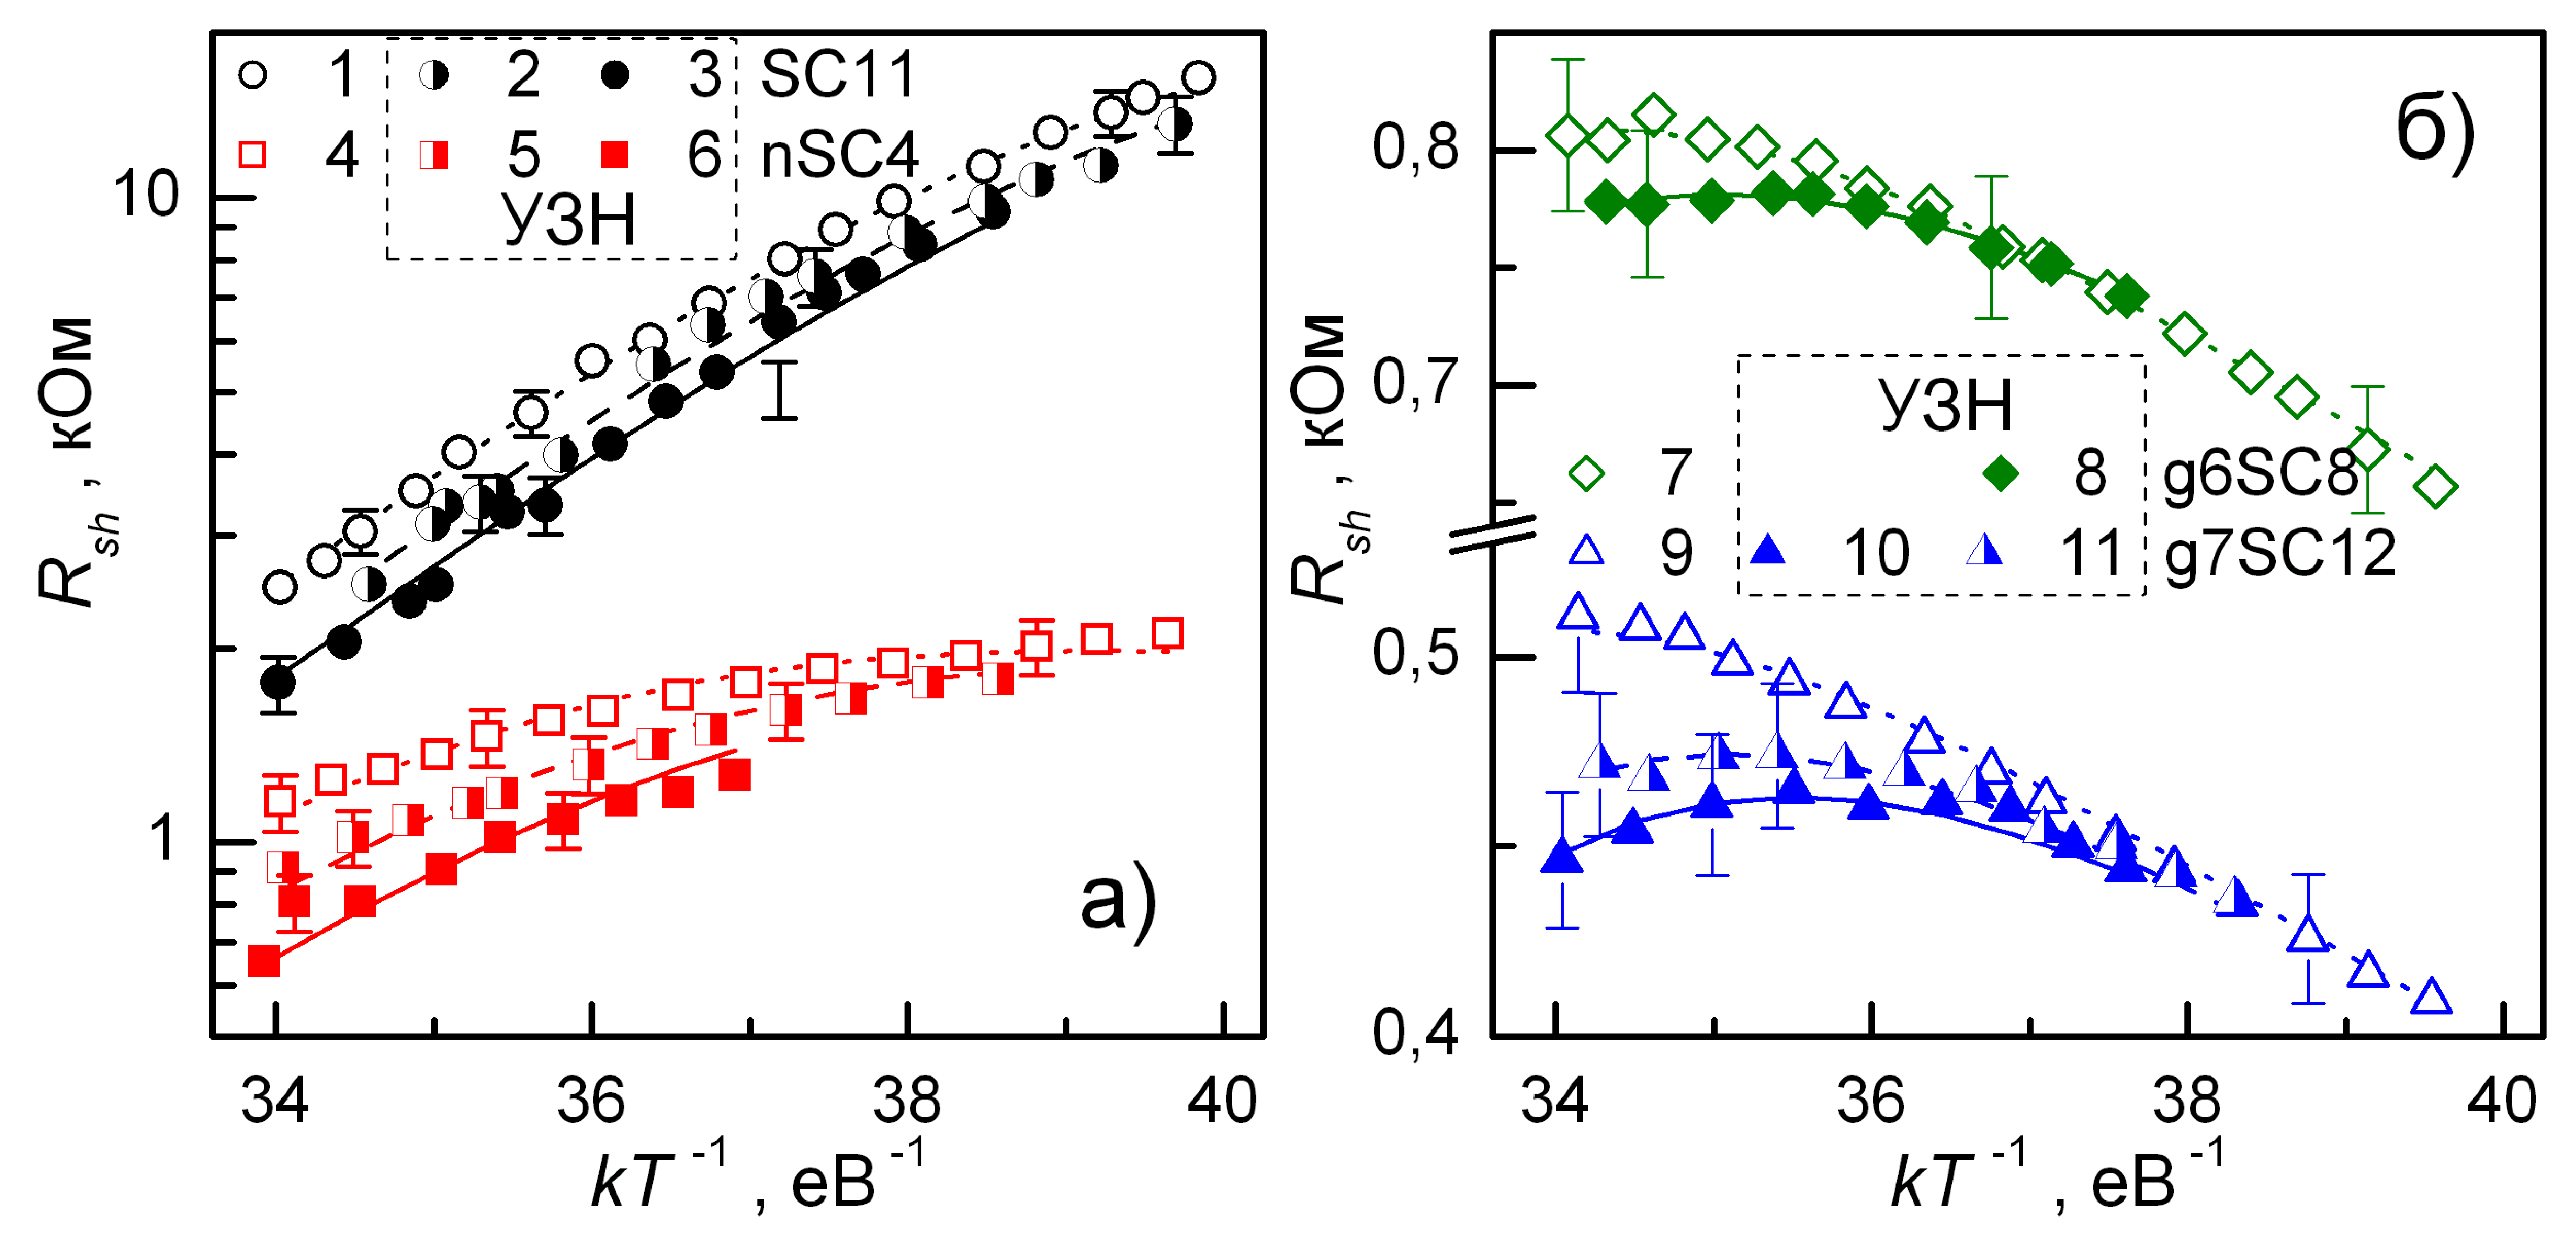
\includegraphics[width=1.0\textwidth]{figRshRD}
\caption{\label{figRshRD}
Температурні залежності величини шунтуючого опору
\FigCaptionSSCRD
%Позначення кривих збігаються з Рис.~\ref{fignRD}.
Точки --- експеримент,
лінії -- результат апроксимації з використанням формул~(\ref{eqRshFull})-(\ref{eqRsh}).
}%
\end{figure}

Відомо \cite{Rsh:Breitenstein,RshMet}, що для появи шунтуючого опору в $p$--$n$ структурах існує декілька причин, не
пов'язаних з механічним ушкодженням.
Так, причиною його появи можуть бути часточки алюмінію, макроскопічні включення Si$_3$N$_4$ або утворення інверсійних шарів
в околі преципітатів.
Проте два останні утворення зустрічаються переважно у мультикристалічних КСЕ \cite{Rsh:Breitenstein} і не можуть
бути причиною шунтуючого опору в досліджених кристалічних зразках.
В той же час вважається, що під час відпалу, необхідного для утворення контактів, частинки Al проникають у зразок,
створюючи навколо себе області з високою концентрацією дірок ($p^+$).
Наявність таких компенсованих областей в емітері КСЕ  забезпечує омічний контакт з базою.

Крім того, в літературі показано \cite{Rsh:Breitenstein,TAT:Gopal,Rsh:Baker,Si:dislIV},
що дислокації, які перетинають область $p$--$n$ переходу, теж можуть бути причиною появи омічного струму.
Наприклад, наявність навіть декількох дислокації в діодних кремнієвих структурах викликає зменшення питомого опору
та зміну форми ВАХ, характерну для підвищення ролі шунтуючого опору \cite{Si:dislIV}.
В досліджених структурах причиною появи дислокацій можуть бути кисневмісні преципітати, при утворенні яких
виникають лінійні дефекти \cite{SiO:Hwang,SiO:Vanhell}, а також напруги, що виникають
на границі сильнолегованої $n$--області та слабколегованої бази.

На нашу думку, в досліджених структурах присутні і дислокації, і частки алюмінію.
В цьому випадку повний шунтуючий опір може бути записаний у вигляді
\begin{equation}
\label{eqRshFull}
R_{sh}^{-1}=R_{sh,\mathtt{Al}}^{-1}+R_{sh,\mathtt{dis}}^{-1}\,,
\end{equation}
де
$R_{sh,\mathtt{Al}}$ та $R_{sh,\mathtt{dis}}$ відображають внески часток алюмінію та дислокацій, відповідно.
Для опору металеву частинки очікується лінійна температурна залежність:
\begin{equation}
\label{eqRshAl}
R_{sh,\mathtt{Al}}=R_{293,\mathtt{Al}}[1+\alpha_R(T-293)]\,,
\end{equation}
де
$R_{293,\mathtt{Al}}$ --- величина шунтуючого опору при 293~K,
а
$\alpha_R$ --- температурний коефіцієнт опору.

З іншого боку, відповідно до моделі дислокаційно--індукованого імпедансу фотовольтаїчних детекторів,
запропонованої в роботах \cite{Rsh:Gopal2003,Rsh:Gopal2004},
$R_{sh,\mathtt{dis}}$ може бути записаний у вигляді:
\begin{equation}
\label{eqRsh}
R_{sh,\mathtt{dis}}=\frac{T}{\sigma_{\mathtt{dis}}}\left[\cosh\left(\frac{E_\mathtt{dis}-E_i}{kT}\right)+\cosh\left(\frac{U_s}{kT}\right)\right]\,,
\end{equation}
де
\begin{equation}
\label{eqRdis}
\sigma_{\mathtt{dis}}=\rho_{\mathtt{dis}}Aq^2A_{\mathtt{dis}}\sqrt{K_nK_p}\,N_{\mathtt{dis}}(n_p+p_p)/k\,,
\end{equation}
$E_{\mathtt{dis}}$ --- енергетичне положення рівня, що відповідає за появу
дислокаційного рекомбінаційного струму;
$U_s$ --- потенціал на поверхні дислокаційного ядра,
$\rho_{\mathtt{dis}}$ та $A_{\mathtt{dis}}$ --- густина та площа поверхні дислокацій,
$K_n$ та $K_p$ --- ймовірності захоплення електронів та дірок дислокаційними станами,
are the probabilities for electrons and holes capture by the dislocation states,
$N_{\mathtt{dis}}$ --- густина поверхневих станів на кожній дислокації.
Вираз~(\ref{eqRsh}) записано для спрощеного випадку $K_p=K_n$.

В роботі температурний коефіцієнт опору був оцінений за даними для зразка g7SC12 в околі кімнатної температури.
Отримана величина $8,3\cdot10^{-3}$~K$^{-1}$ не дуже суттєво відрізняється від температурного
коефіцієнту опору об'ємного алюмінію ($4,3\cdot10^{-3}$~K$^{-1}$),
що підтверджує доцільність зроблених припущень.
Надалі, використовуючи отримане значення $\alpha_R$, була
проведена апроксимація температурних залежностей $R_{sh}$ відповідно до формул (\ref{eqRshFull})--(\ref{eqRsh}).
При цьому шуканими параметрами вважалися $R_{293,\mathtt{Al}}$, $(E_{\mathtt{dis}}-E_i)$, $U_s$ та $\sigma_{\mathtt{dis}}$.
Виявилось, що експериментальні залежності добре описуються апроксимуючими кривими (див. Рис.~\ref{figRshRD})
при значеннях $(E_{\mathtt{dis}}-E_i)=(0.46\pm0.02)$~еВ та $U_s=(5\pm4)\times10^{-8}$~еВ,
причому ці величини не залежать від опромінення та УЗН.
Отримана величина $(E_{\mathtt{dis}}-E_i)$ відповідає енергії активації носіїв $0.10\pm0.02$~еВ.
Це, в свою чергу, досить близько до енергії активації дислокаційних рівнів $0.08$~еВ,
яка спостерігалася раніше \cite{disl10:Castaldini,disl10:Isakova,disl10:Yur,disl10:Kveder,disl10:Trushin,Si:disl},
у тому числі і в Cz--Si:B \cite{disl10:Castaldini,disl10:Isakova,disl10:Yu}.
Зауважимо, що дислокаціям в напівпровідникових кристалах відповідають як мілкі,
так і глибокі рівні \cite{Disl:GaN};
якщо в параграфі~\ref{sBulyrMethod} акцент було зроблено на глибокі, то на шунтуючий опір, як виявилося,
переважний вплив мають мілкі.


Отримані значення $R_{293,\mathtt{Al}}$ та $\sigma_{\mathtt{dis}}$ наведено в Таблиці~\ref{tabSSCparRD}.
$R_{293,\mathtt{Al}}$ не залежить від УЗН та зростає з опроміненням.
На нашу думку, виявлена зміна характеру температурної залежності шунтуючого опору пояснюється
наступним чином.
Для неопромінених зразків $R_{sh,\mathtt{dis}}$ менший ніж $R_{sh,\mathtt{Al}}$ і шунтуючий опір
у структурі визначається насамперед рекомбінацією на дислокаціях, які перетинають площину $p-n$ переходу,
утворюючи канали для проходження носіїв заряду.
При опроміненні утворюються вакансії, що полегшує дифузію атомів Al з електродів, насамперед з фронтального у емітер.
В результаті кількість часточок Al та їх розмір зростає, $R_{sh,\mathtt{Al}}$ зменшується,
перетворюючись при високих дозах на ключовий фактор визначення повного шунтуючого опору.
Дифузія Al у $\gamma$--опромінених зразках відбувається більш ефективно через те, що
 при такому способі впливу утворюються окремі рівномірно розподілені по об'єму вакансії, тоді
 як при нейтронному опроміненні виникають рідко розташовані вакансійні кластери.
Як наслідок, в nSC4 величина $R_{sh,\mathtt{Al}}$ хоч і зменшується, проте залишається
більшою ніж дислокаційно--індукований опір на відміну від $\gamma$--опромінених зразків.

Розкид $\sigma_{\mathtt{dis}}$ в наборі зразків корелює з дисперсією $\tau_n$ --- див. параграф~\ref{sbRadDef}.
Отже, відмінності $\sigma_{\mathtt{dis}}$ також пов'язані з неоднорідністю
властивостей вихідної пластини.
УЗН викликає збільшення $\sigma_{\mathtt{dis}}$, відносні величина АІ змін
наведено в Таблиці~\ref{tabAIchangeRD}.
На нашу думку, ці зміни пов'язані зі зростанням величини $A_\mathtt{dis}$ під час поширення АХ.
Дійсно, під час УЗН з використанням поперечних та повздовжніх хвиль,
атоми у ядрі дислокації коливаються перпендикулярно та паралельно, відповідно, напрямку поширення струму.
У результаті в першому випадку на дислокаційні рівні носії захоплюються зі збільшеного об'єму,
ефективна площа поверхні зростає і $R_{sh,\mathtt{dis}}$ зменшується внаслідок дії УЗ.
При використанні повздовжніх хвиль процес проходить менш ефективно і АІ впливу на величину
шунтуючого опору при такому УЗН не спостерігається (Рис.~~\ref{figDUS_Rsh}).

\subsection{Особливості впливу ультразвукового навантаження на фотогенерацію струму в нейтронно--опромінених структурах\label{sbNIsc}}

Для оцінки фотоелектричного перетворення в роботі також проводились вимірювання фотогенерованого струму
в радіаційно--опромінених структурах
при монохроматичному освітленні в режимі короткого замикання КСЕ (замість вимірювання повної ВАХ).
На Рис.~\ref{figIscRD} наведено отримані температурні залежності фотоструму (струму короткого замикання)
за умов УЗН та при нагріванні без збудження АХ.
Криві 1 та 2 взяті з Рис.~\ref{figDUSIsc}.




\begin{figure}[b]
\center
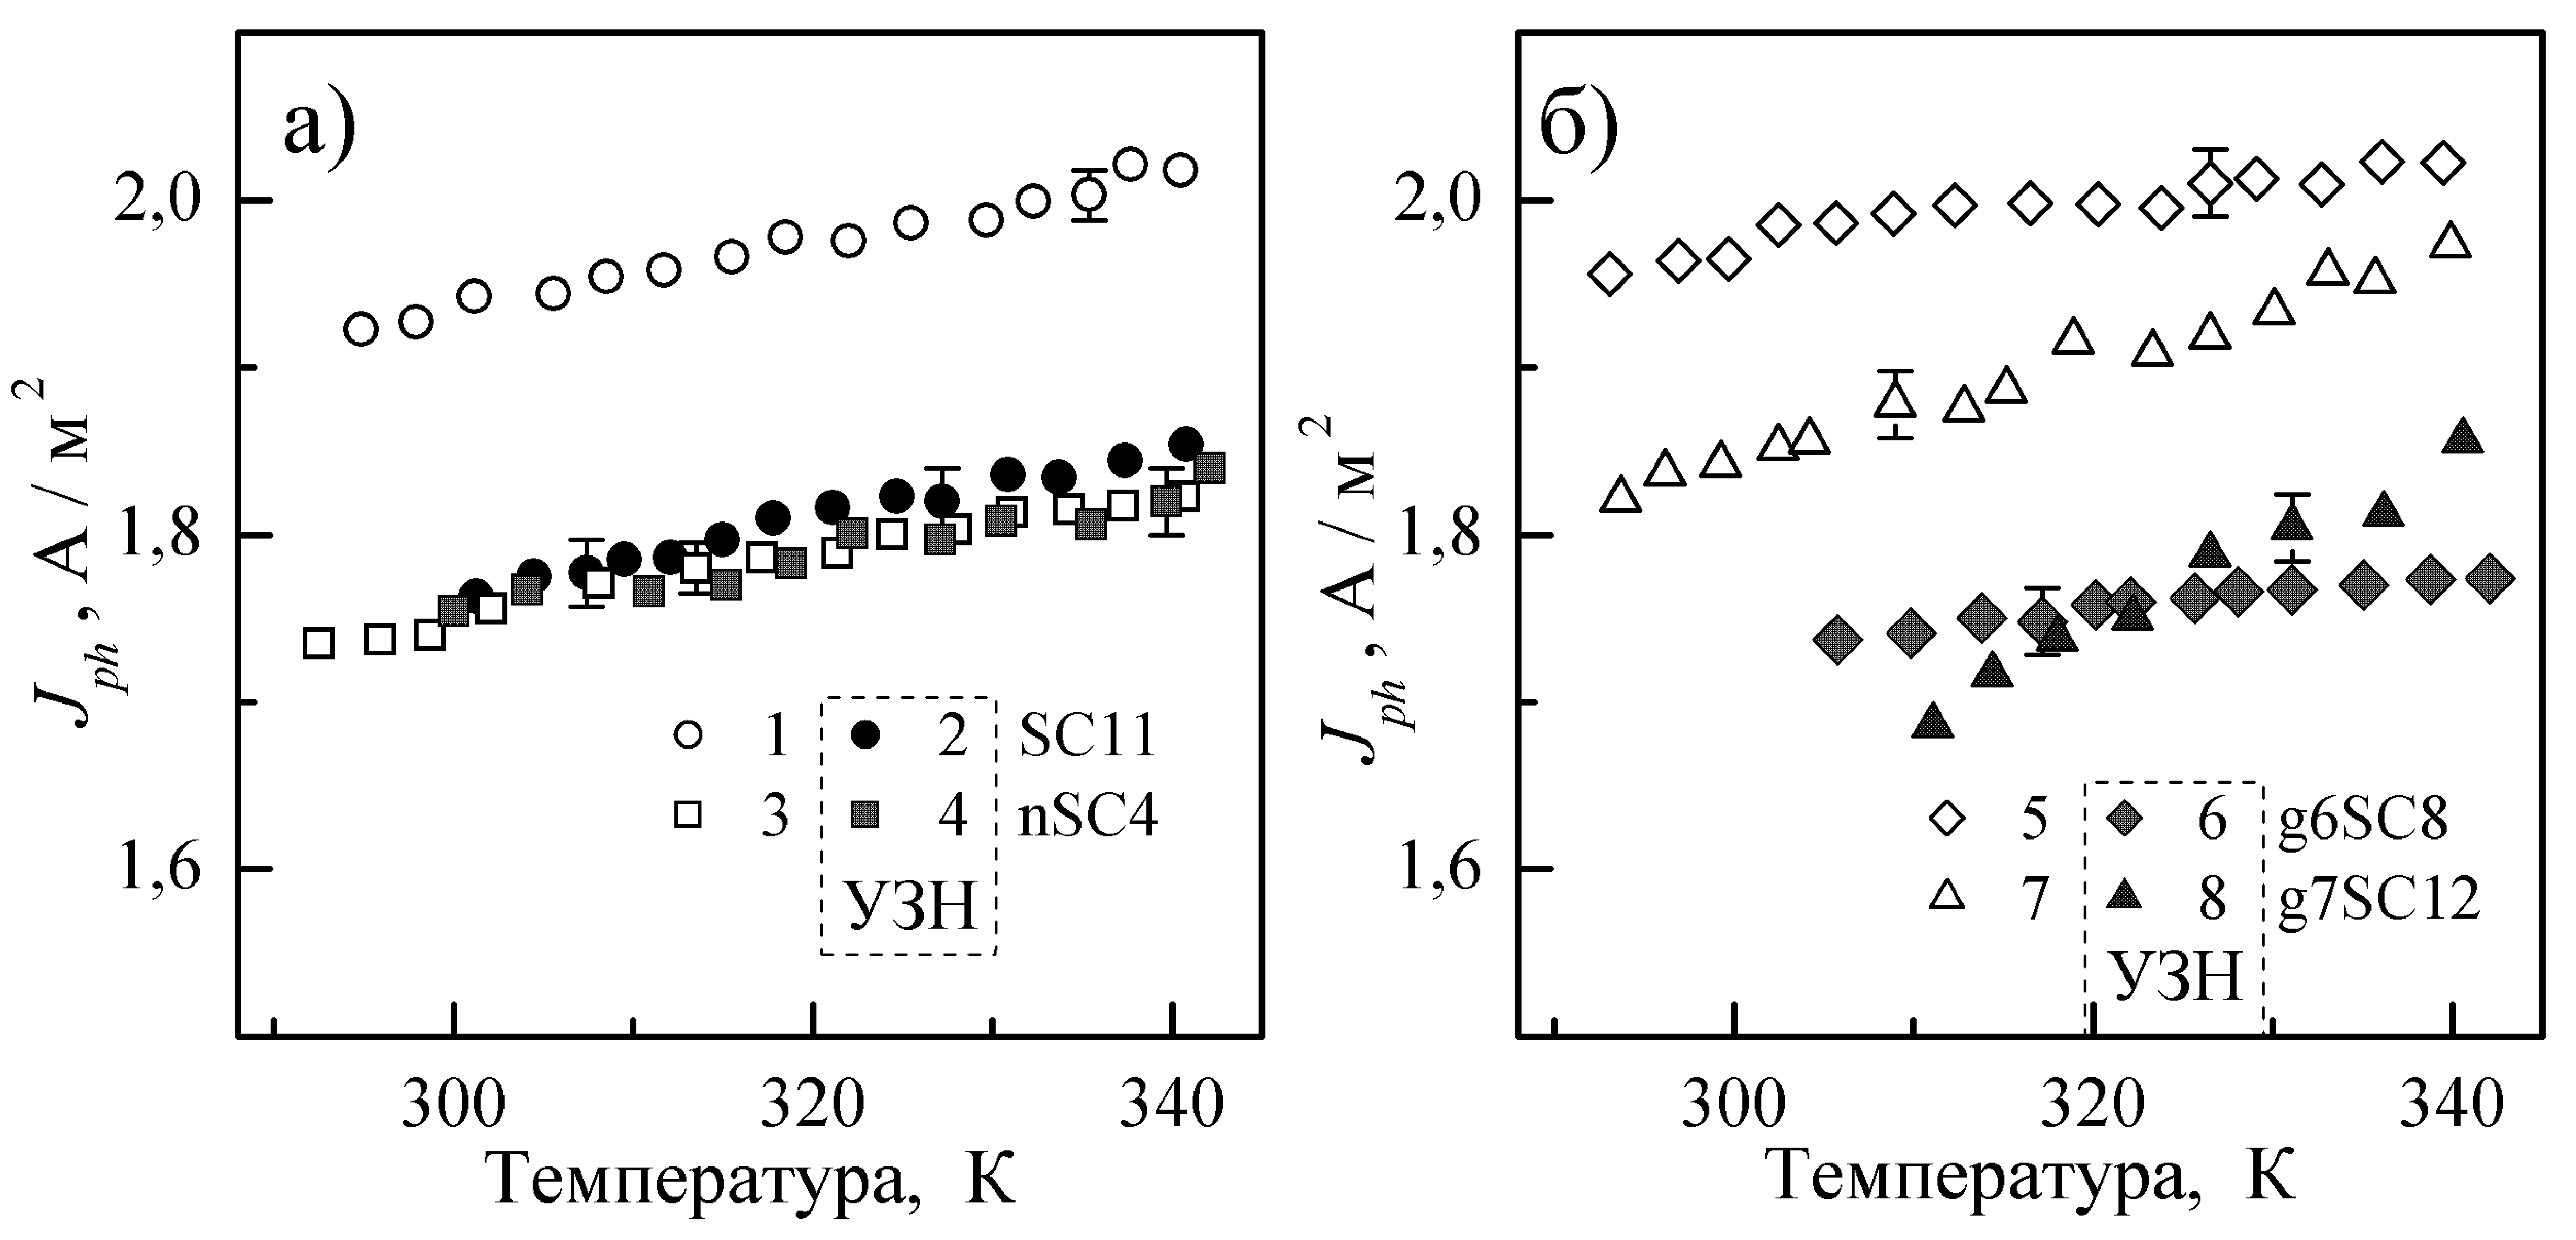
\includegraphics[width=1.0\textwidth]{figIscRD}
\caption{\label{figIscRD}
Температурні залежності густини фотоструму
для неопроміненого (криві 1 та 2, кола),
нейтронно--опроміненого (3 та 4, квадрати) та
гамма--опромінених (5--8, ромби та трикутники)
зразків.
Криві 1, 3, 5 та 7 (незаповнені точки) отримані без УЗН,
криві 2 та 4 відповідають УЗН U--Tb3,
6 та 8 ---
U--Tb2 та U--Tb1, відповідно.
}%
\end{figure}

З рисунка видно, що при збільшенні температури $J_{ph}$ зростає як до радіаційного впливу, так і після.
З літератури \cite{Faren,SCTemp:PP11,SCTemp:SEMSC140} відомо, що
подібна поведінка фотоструму зумовлена, переважно, двома факторами:
\begin{enumerate}[label=\arabic*),leftmargin=0em,itemindent=1.5em]
\item зменшення забороненої кристалу та зміною коефіцієнта поглинання світла;
\item збільшенням довжини дифузії неосновних носіїв заряду.
\end{enumerate}
Показано \cite{SCTemp:PP11,SCTemp:SEMSC140}, що при аналізі температурної залежності доцільно
розглядати густину фотоструму у вигляді
\begin{equation}
\label{eqIscIdeal}
J_{ph}=J_{Lg}f_c\,,
\end{equation}
де
$J_{Lg}$ --- ідеальне значення густини струму, яке визначається
зонною структурою кристалу,
$f_c$ --- коефіцієнт збирання (collection fraction),
який залежить від відбиття світла, його паразитного поглинання (особливо вільними носіями заряду)
та поширення носіїв у кристалі.
В цьому випадку температурний коефіцієнт фотоструму $\beta^T_{Jph}$ може бути записаний у вигляді
\begin{equation}
\label{eqIscTempKoef}
\beta^T_{Jph}=\frac{1}{J_{ph}}\frac{dJ_{ph}}{dT}=\frac{1}{J_{Lg}}\,\frac{dJ_{Lg}}{dE_g}\,\frac{dE_g}{dT}+\frac{1}{f_{f}}\frac{df_{c}}{dT}\,,
\end{equation}
причому перший доданок для кремнію у випадку сонячного освітлення становить близько $167\cdot10^{-6}$~K$^{-1}$.

Визначені з експерименту значення температурних коефіцієнтів наведено в Таблиці~\ref{tabIscT}.
Видно, що у всіх випадках зміна $J_{ph}$ з температурою визначається, насамперед,
зміною $f_c$, а величина $\beta^T_{Jph}$ практично не залежить від УЗН (за винятком інтенсивно опроміненого опроміненого гамма--квантами зразка).

\begin{table}
\caption{\label{tabIscT}Температурний коефіцієнт струму короткого замикання.
}
\center
\begin{tabular}{|c|c|c|c|}
\hline
Зразок&\multicolumn{2}{c|}{$\beta^T_{Jph}$, 10$^{-3}$K$^{-1}$}&УЗН\\ \cline{2-3}
&без УЗН & зі УЗН&\\ \hline
SC11&$1,3\pm0,2$&$1,2\pm0,2$&U--Tb3\\ \hline
nSC4&$1,1\pm0,2$&$1,3\pm0,3$&U--Tb3\\ \hline
g6SC8&$0,8\pm0,2$&$0,6\pm0,1$&U--Tb2\\ \hline
g7SC12&$1,6\pm0,2$&$3,1\pm0,4$&U--Tb1\\ \hline
\end{tabular}
\end{table}

На Рис.~\ref{figIscRD} звертає на себе увагу той факт, що у нейтронно--опроміненому
зразку фактично не спостерігається зміни величини фотоструму під дією УЗН.
Цей результат є досить несподіваним, враховуючи те, що, як було показано раніше,
УЗ викликає зменшення часу життя неосновних носіїв в КНО і в нейтронно--опроміненому зразку також ---
див. Рис.~\ref{figTAUrRD}, Таблицю~\ref{tabAIchangeRD}.
Причому ефективність АІ змін $\tau_n$ в нейтронно--опроміненому зразку навіть вища (Таблиця~\ref{tabAIchangeRD}, Рис.~\ref{figKusRD}),
що, як було показано в параграфі~\ref{sbRadDef}, зв'язано з акусто--активністю дивакансії.

На Рис.~\ref{figeIscRD} наведено більш детальне порівняння АІ змін фотоструму в нейтронно--опроміненому та неопроміненому
зразках при різних режимах УЗН з використанням повздовжніх хвиль.
З рисунка видно, $J_{ph}$ зменшується (нагадаємо, що, як і для всіх інших параметрів, $\varepsilon_{Jph}=(J_{ph,in}-J_{ph,\mathtt{US}})/{J_{ph,in}})$) при цьому
\begin{enumerate}[label=\asbuk*),leftmargin=0em,itemindent=1.5em]
\item зі збільшенням частоти УЗ ефективність змін фотоструму в неопроміненому КСЕ зростає;
\item навіть при високих частотах АІ ефект впливу УЗ на $J_{ph}$ в нейтронно--опроміненому КСЕ достатньо малий.
\end{enumerate}


\begin{figure}
\center
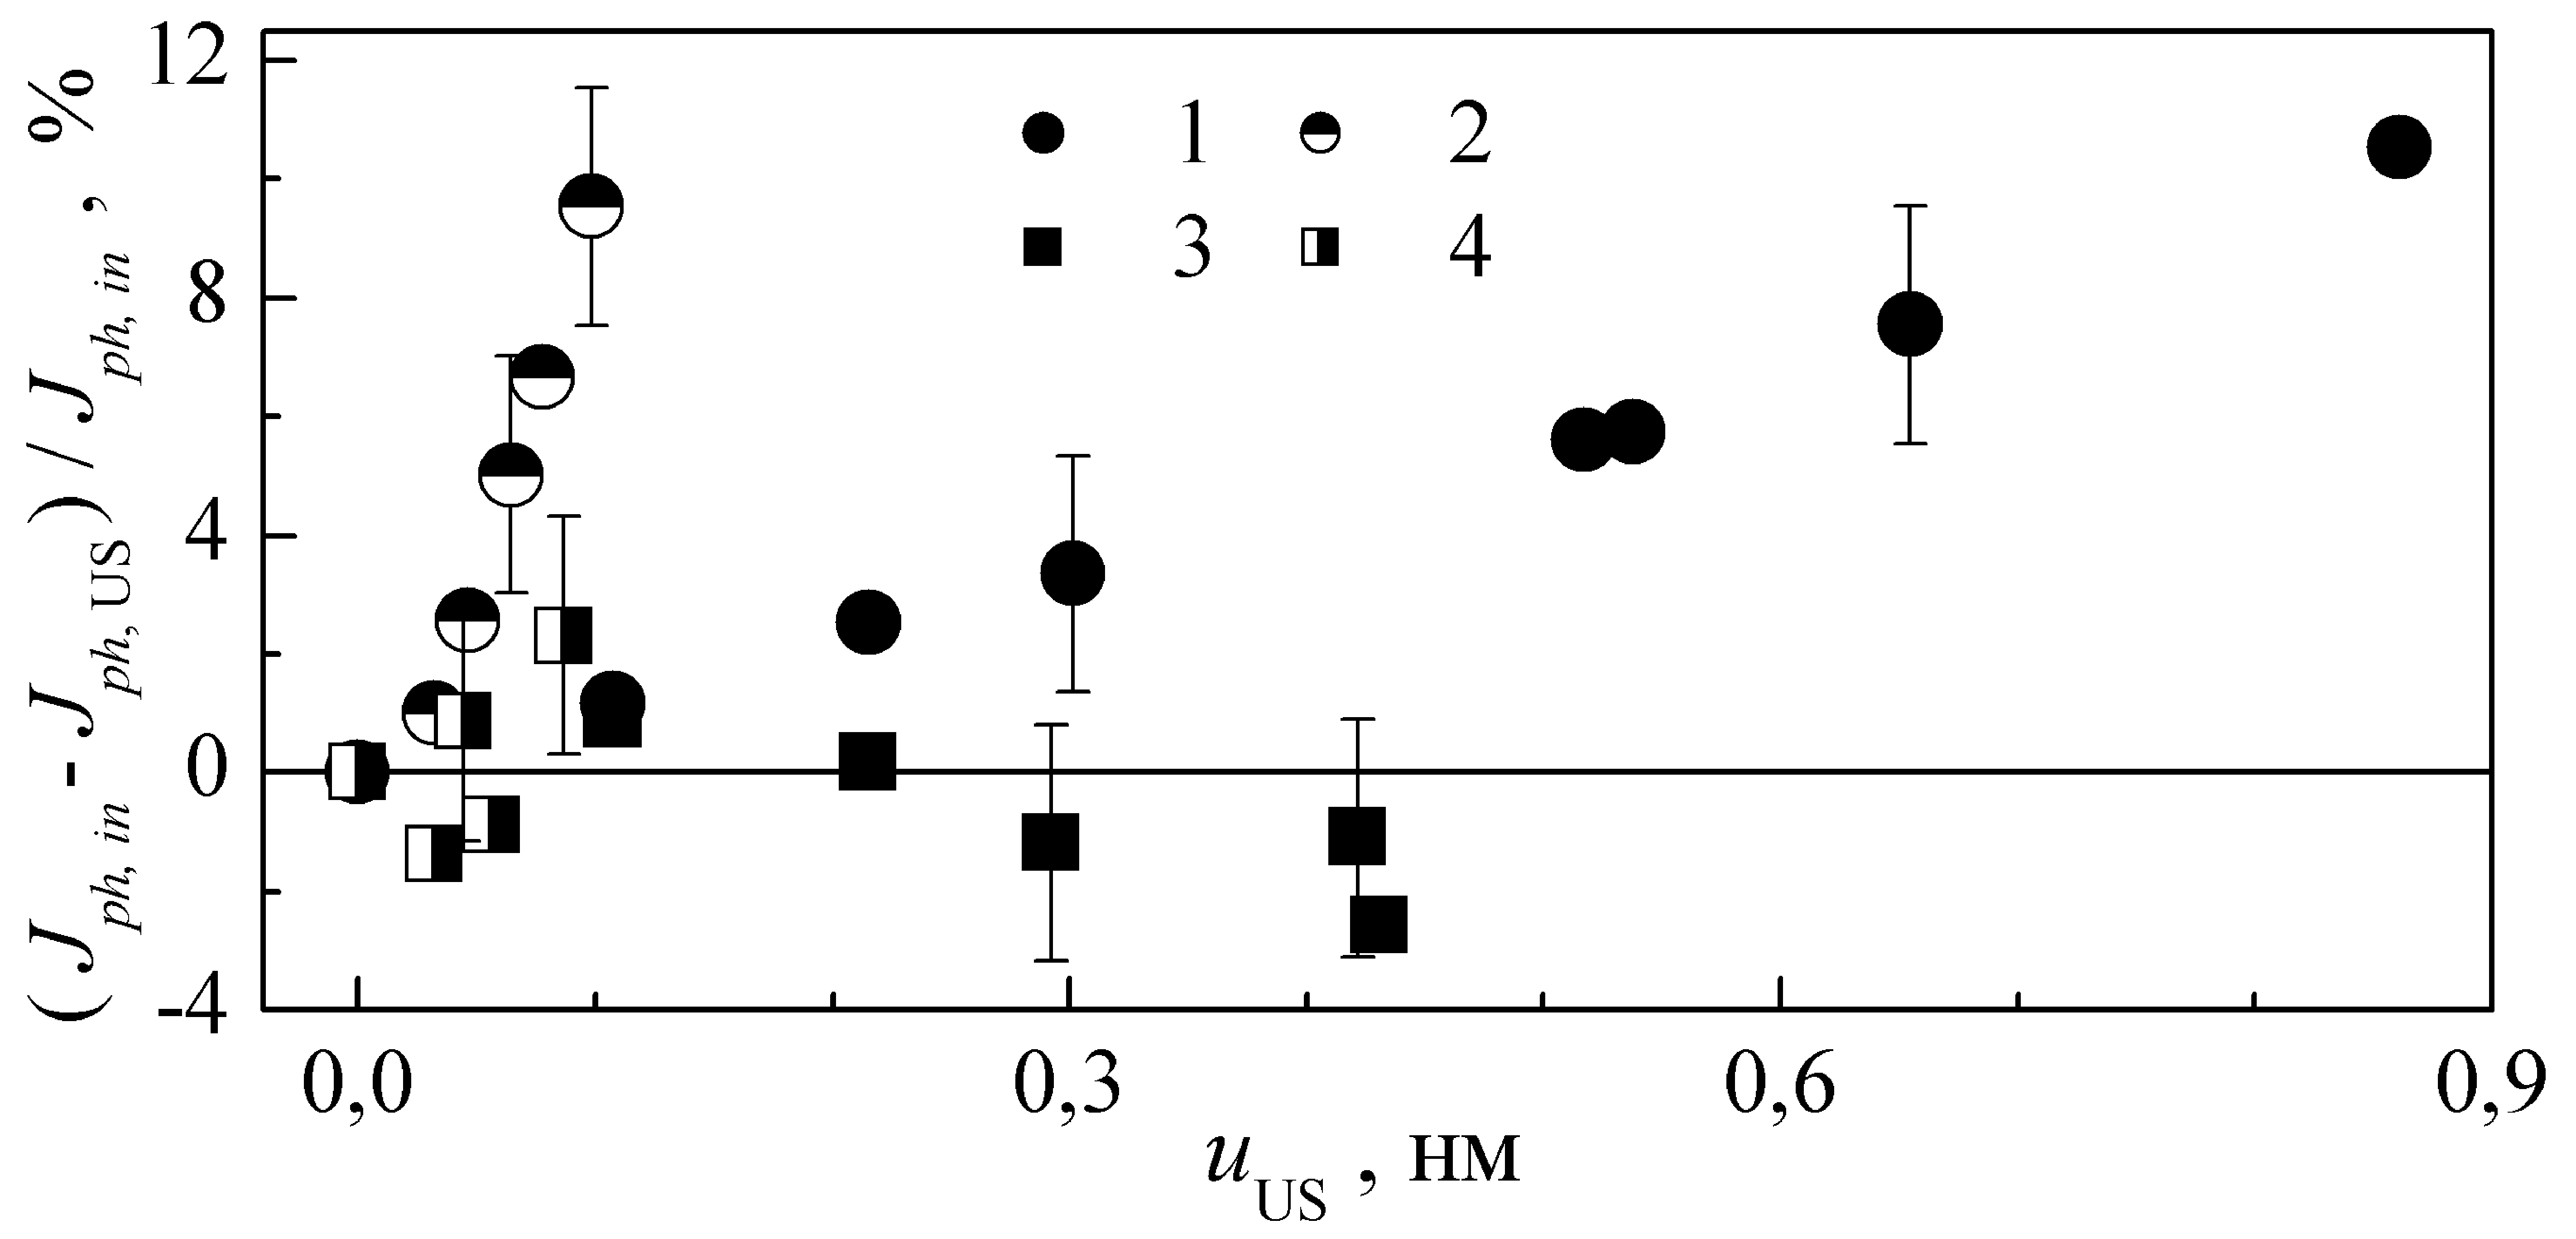
\includegraphics[width=1.0\textwidth]{figeIscRD}
\caption{\label{figeIscRD}
Залежності АІ змін фотоструму від
амплітуди зміщень атомів в неопроміненому (кола)
та опроміненому (квадрати) зразках.
$f_\mathtt{US}$, Гц: 8,0 (U--L8, заповнені точки),
26,1 (U--L26, напівзаповнені точки).
}%
\end{figure}

З метою більш детального вивчення виявленої особливості було проведено дослідження змін
довжини дифузії неосновних носіїв заряду.
Для визначення $L_n$ використовувався варіант методу SSSCC (steady--state short--circuit current)\cite{Schroder2006}.
А саме, як вже було згадано раніше, величина фотоструму в досліджених структурах
описується виразом (\ref{eqIph}).
Тобто, $J_{ph}$ має лінійно залежати від кількості фотонів
\mbox{$N_{ph}=W_{ph}\lambda /hc$}, які падають на поверхню структури за одиницю часу:
\begin{equation}
J_{ph}=K_{ph}N_{ph}\,,
\end{equation}
де коефіцієнт пропорційності
\begin{equation}
 K_{ph}=\frac{(1-R_{ph})\,q\beta \alpha L_n} {1+\alpha L_n}\,.
\end{equation}
Таким чином, знаючи коефіцієнти $K_{ph1}$ та $K_{ph2}$
для двох довжин хвиль $\lambda_1$ і $\lambda_2$, можна
визначити $L_n$:
\begin{equation}\label{F3}
L_n=\frac{(K_{ph1}\alpha_2)/(K_{ph2}\alpha_1)-1}{\alpha_2(1-K_{ph1}/K_{ph2})}\,,
\end{equation}
де $\alpha_1$ та $\alpha_2$ --- коефіцієнти поглинання для
світла з довжиною хвилі $\lambda_1$ та $\lambda_2$, відповідно.

В роботі використовувалися довжини світла 900 та 950 нм,
попереднє калібрування величини $W_{ph}$ здійснювалось
за допомогою германієвого фотодіоду 9Э111А.
На Рис.~\ref{figIscNph} показано типові залежності фотоструму від
кількості падаючих фотонів для двох довжин хвиль,
які дійсно були лінійні.
Зауважимо, що вираз (\ref{F3}) є справедливим,
за умови, що $R_{ph}$ та $\beta$ є однаковими для обох довжин.
Проте з літератури відомо, що для використаних довжин хвиль
$\beta=1$ \cite{Gaman}, а зміна коефіцієнту відбивання не перевищує 1\% \cite{GreenOptic,SiOptic:JAP1998,GreenOptic2}.
Таким чином, для визначення $L_n$ використовувалася формула (\ref{F3}),
причому $K_{ph1}$ та $K_{ph2}$ були виміряні експериментально, а значення
коефіцієнтів поглинання обчислювалися за допомогою виразу (\ref{eqAlpha}).

\begin{figure}
\center
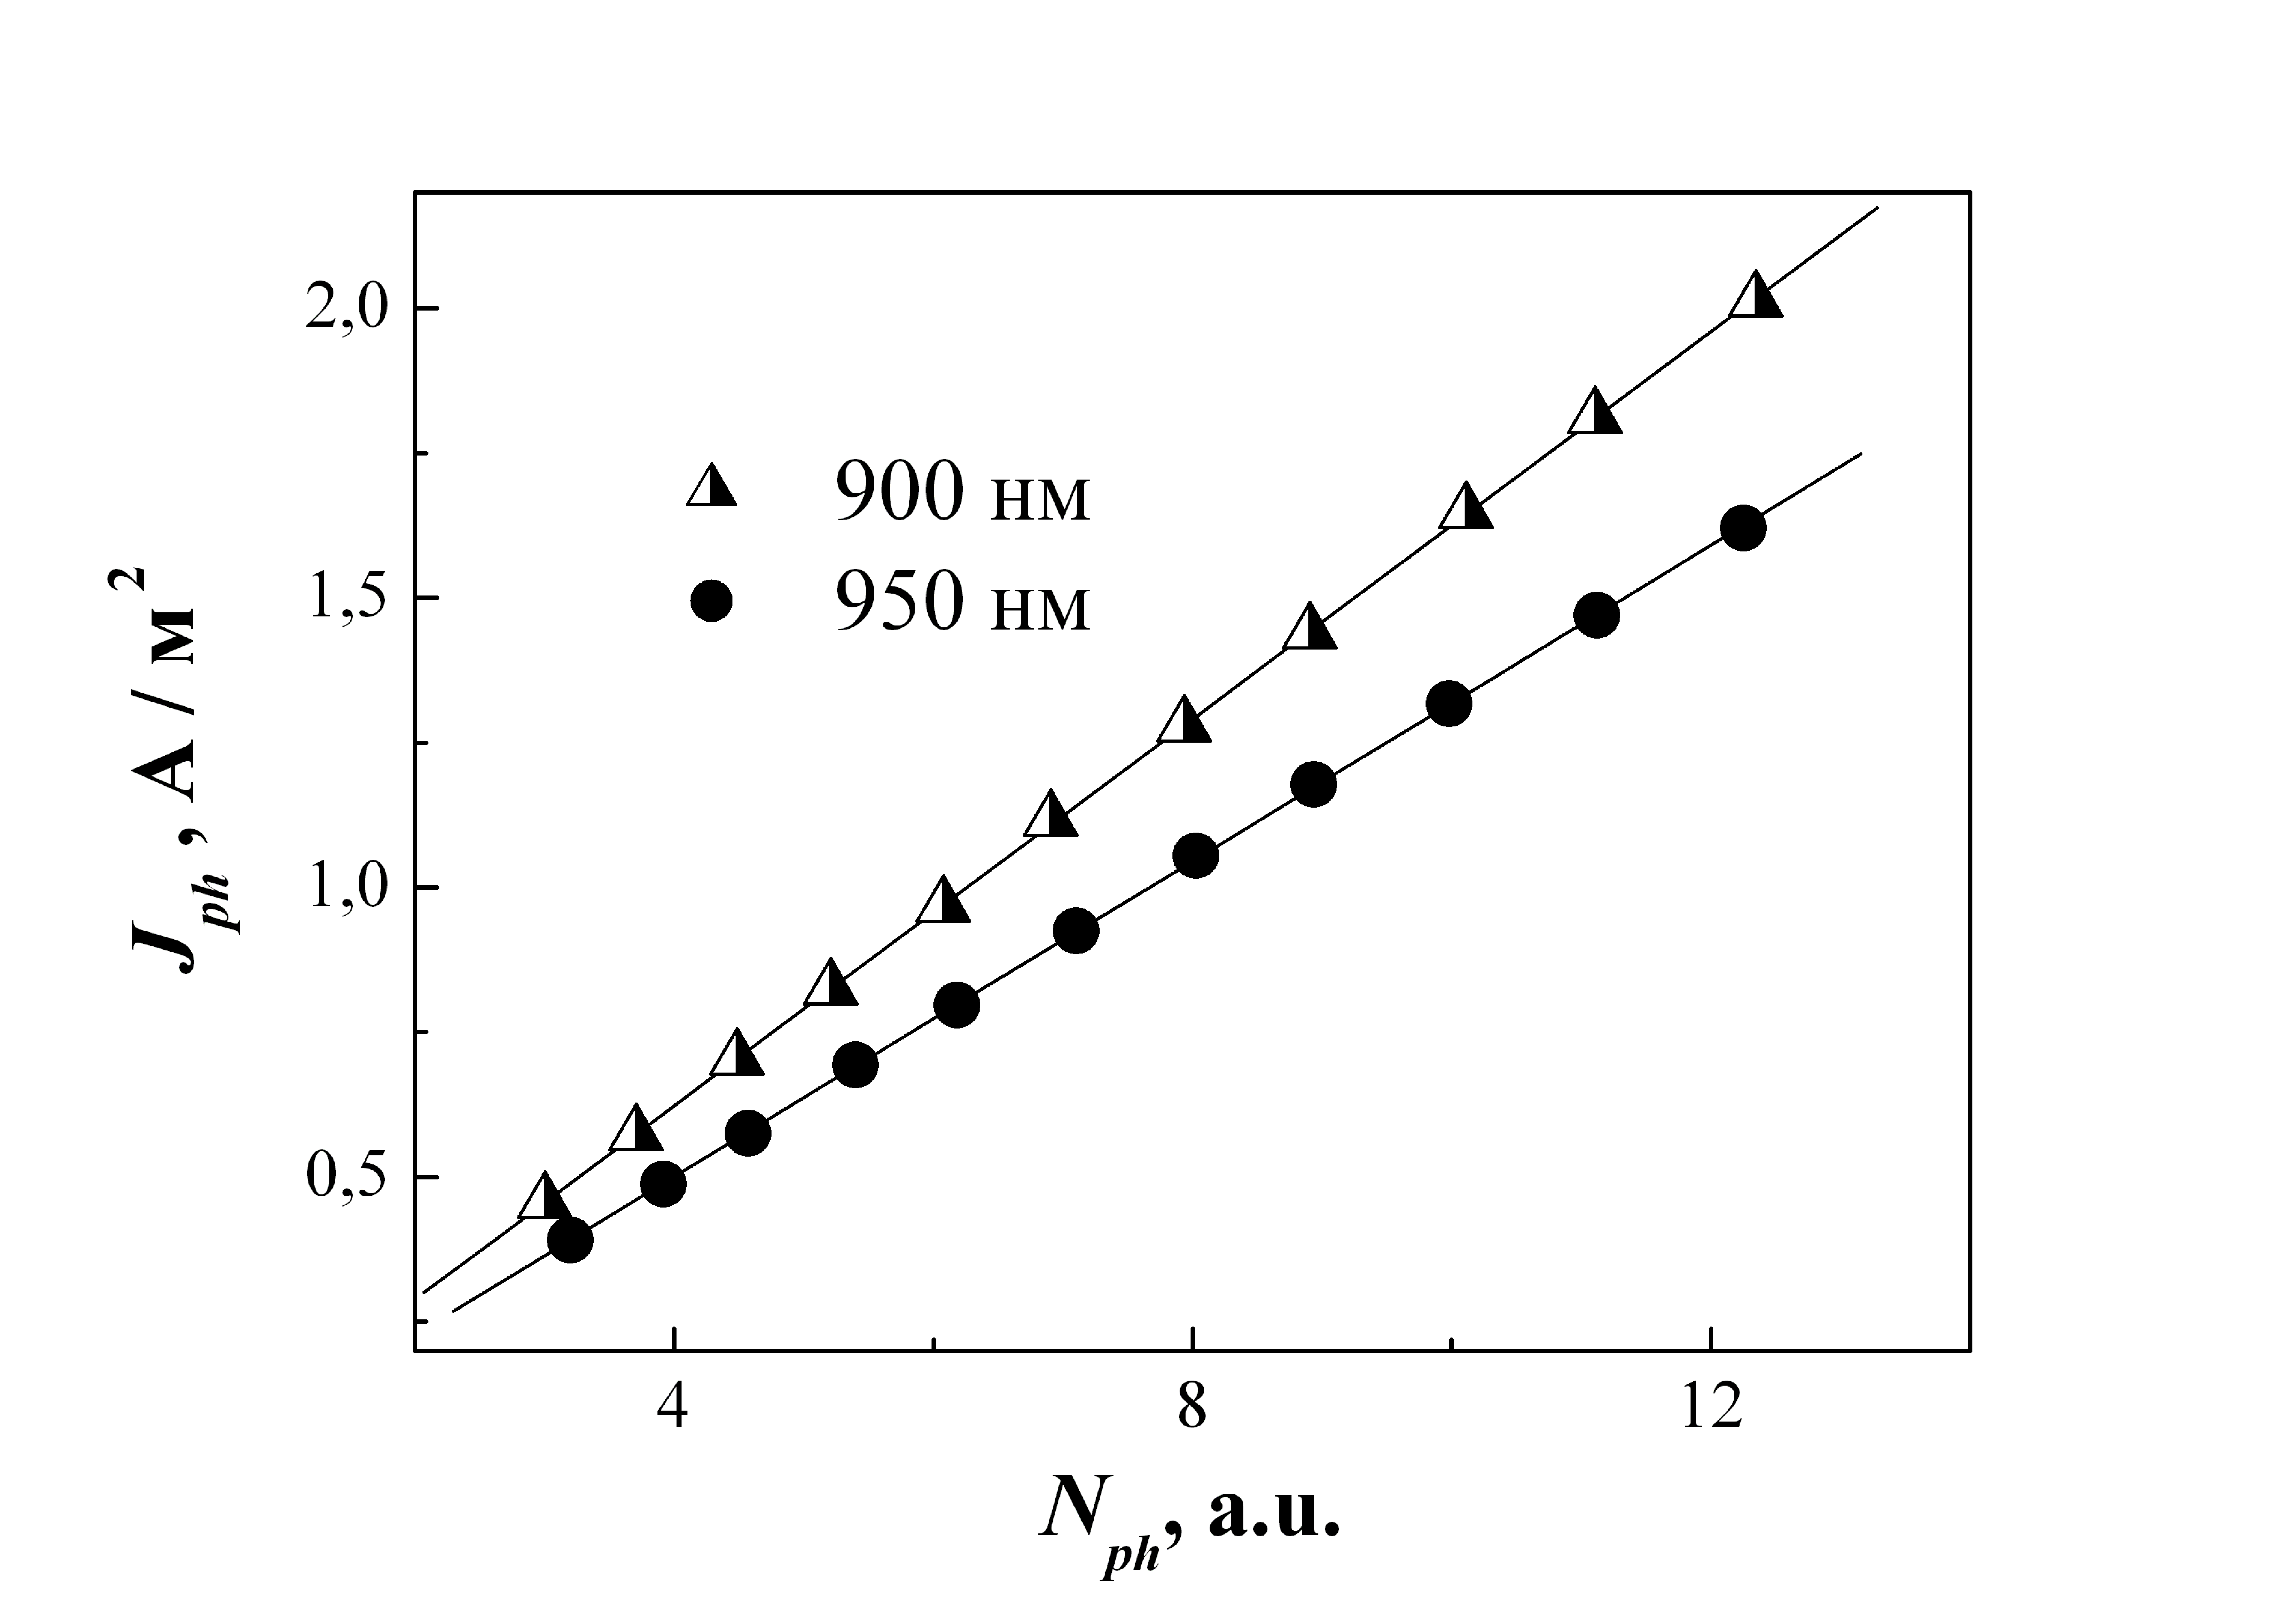
\includegraphics[width=0.7\textwidth]{figIscNph}
\caption{\label{figIscNph}
Залежність густини фотоструму від кількості падаючих фотонів.
Точки – експеримент, лінії – лінійна апроксимація.
$\lambda$, нм: 900 (трикутники), 950 (кола). Зразок SC13. $T = 290$~К.
}%
\end{figure}

З виразу (\ref{eqIph}) випливає, що при незалежності $R_{ph}$ від температури
зміна $J_{ph}$ має визначатися зміною
коефіцієнта $\Gamma=\alpha\,L_n/(1+\alpha\,L_n)$.
Було проведене порівняння відносних змін
фотоструму при нагріванні $\varepsilon^T_{Jph}=[J_{ph}(T)-J_{ph}(T_0)]/J_{ph}(T_0)$
($T_0=290$~K)
з відносними змінами цього коефіцієнта $\varepsilon_\Gamma=[\Gamma(T)-\Gamma(T_0)]/\Gamma(T_0)$,
при обчисленні якого використовувалися значення  $L_n$, визначені
для тих самих температур, при яких проводилось вимірювання $J_{ph}$.
Отримані результати показано на Рис.~\ref{figeIsceG}.


\begin{figure}
\center
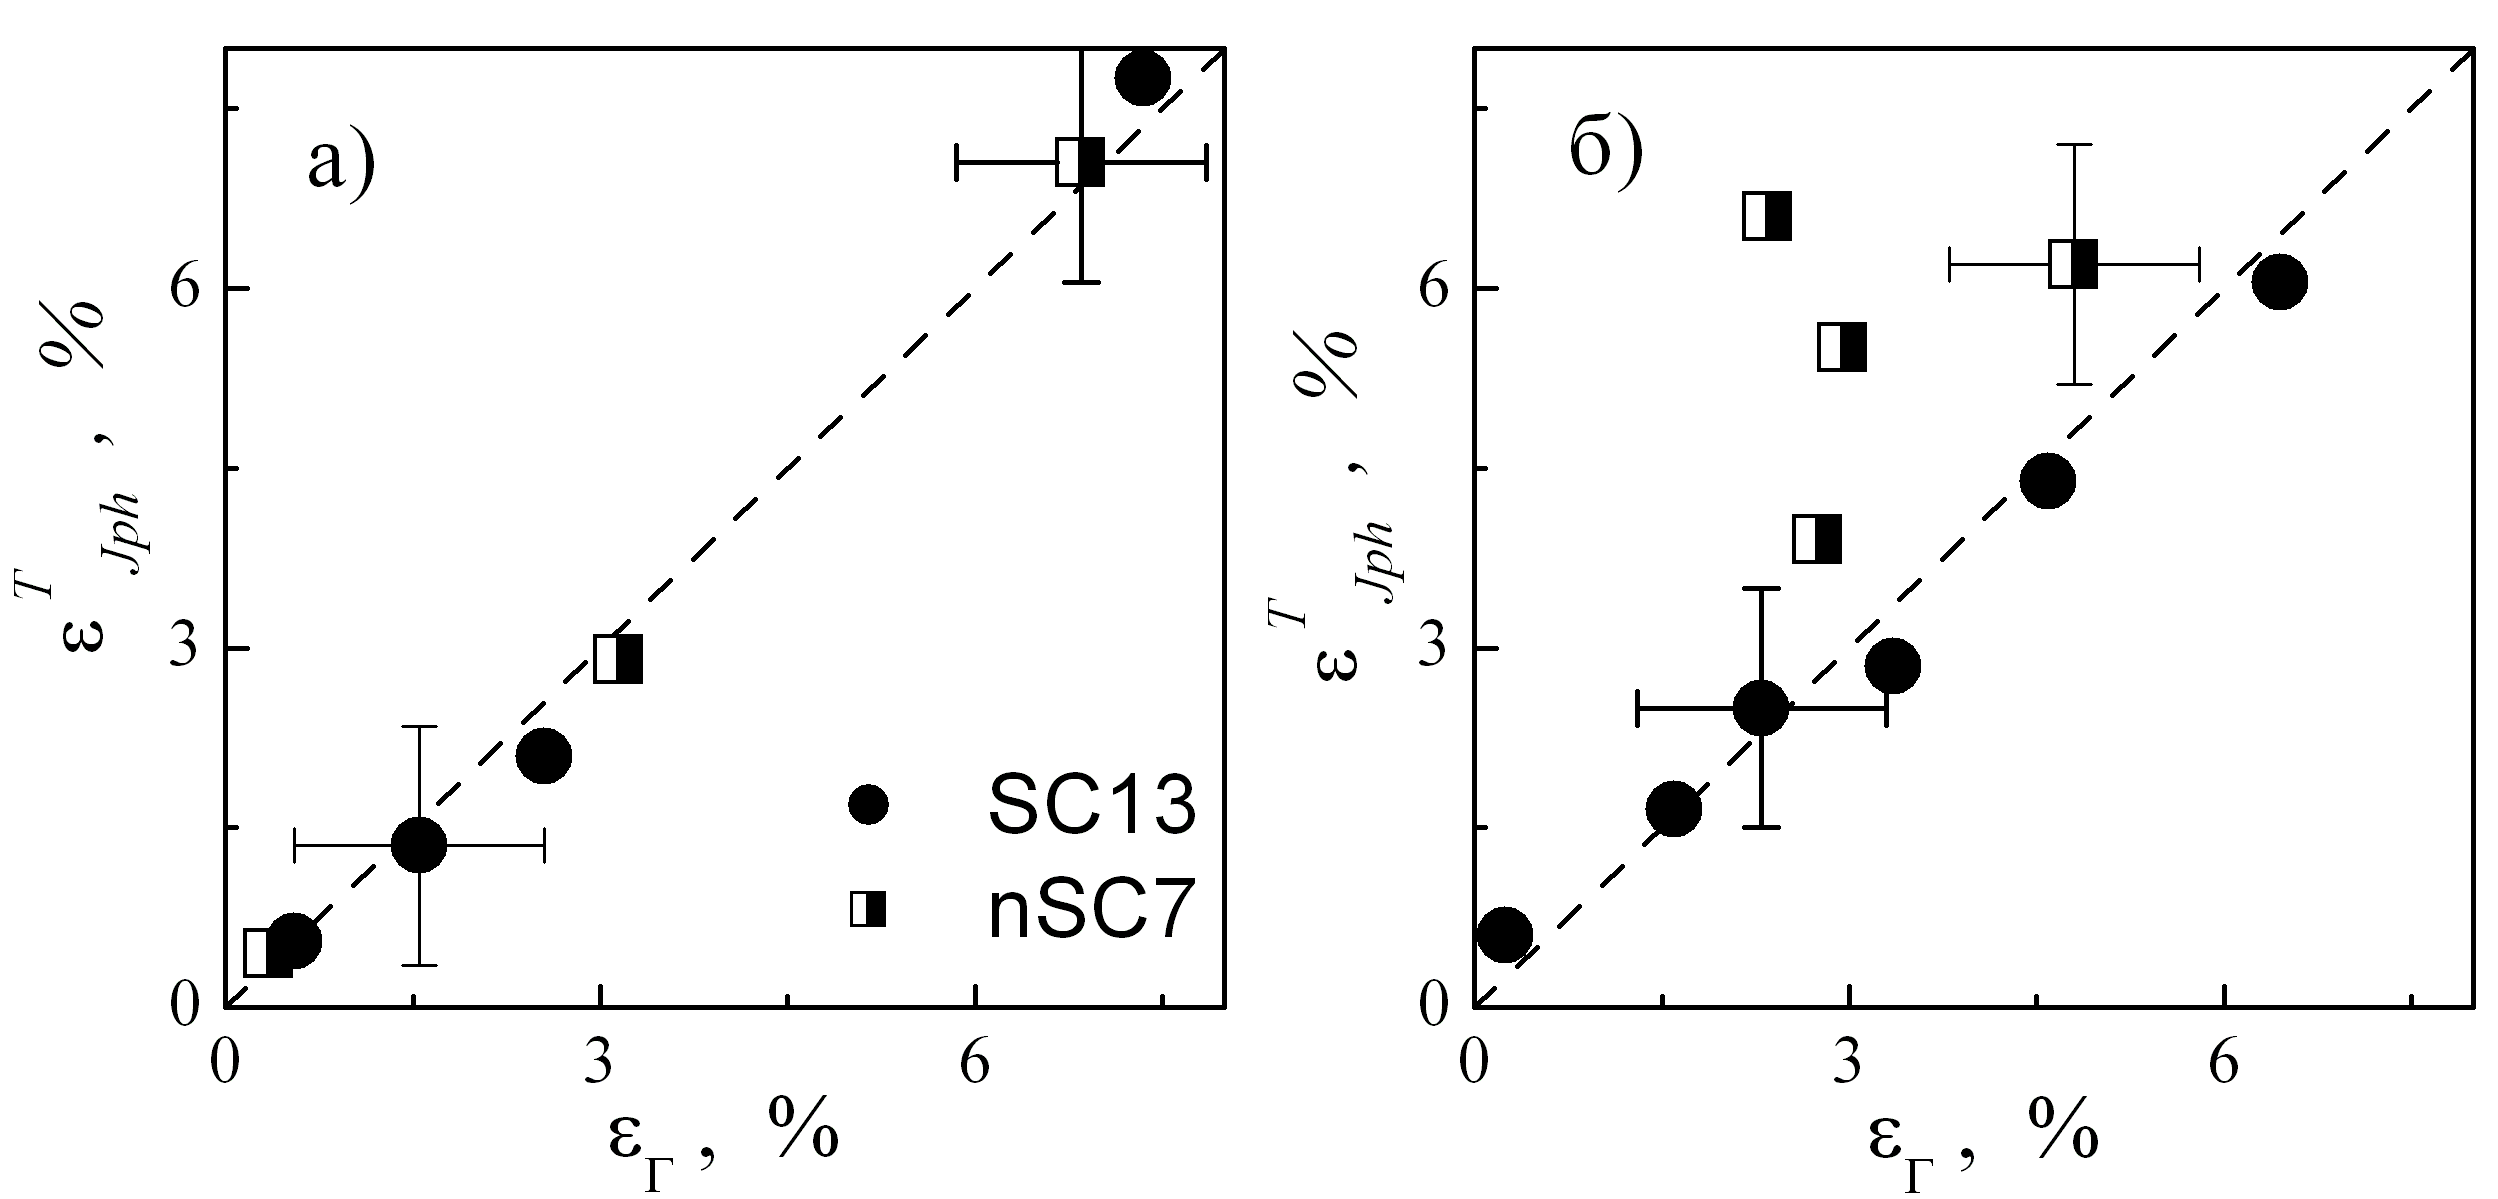
\includegraphics[width=1.0\textwidth]{figeIsceG}
\caption{\label{figeIsceG}
Порівняння відносних змін фотоструму зі змінами довжини
вільного пробігу неосновних носіїв заряду при беззвуковому
нагріванні (а) та нагріванні під час УЗН (U--L8, б)
для неопроміненого (кола) та опроміненого (квадрати) зразків.
}%
\end{figure}

Наведені дані показують, що при нагріванні за відсутності УЗН і для неопроміненого,
і для нейтронно--опроміненого зразка зміна фотоструму визначається зміною
$L_n$:
точки на Рис.~\ref{figeIsceG},а розташовані дуже близько до діагоналі.
Подібна картина спостерігається і для неопроміненого зразка в
умовах УЗН (Рис.~\ref{figeIsceG},б).
Тобто, зміна фотоструму в цьому випадку пов'язана з АІ зменшенням
довжини дифузії (часу життя) неосновних носіїв заряду в квазі--нейтральній
області внаслідок перебудови акусто--активних рекомбінаційних центрів ---
ефект, розглянутий раніше.
Збільшення ефективності АІ змін зі зростанням частоти УЗ, яке
спостерігається в експериментах, може бути пов'язане з наближенням
$f_\mathtt{US}$ до власних частот коливань домішкового комплексу.
Подібний резонансний характер АДВ спостерігався і раніше \cite{Ol_Shav}.




Водночас у нейтронно--опромінених структурах зміна фотоструму при УЗН більша,
ніж це можна очікувати виходячи зі значень зміни коефіцієнта $\Gamma$, пов’язаних з АІ зростанням $L_n$ --- Рис.~\ref{figeIsceG},б.
Це свідчить про існування додаткового механізму впливу УЗ на генерацію фотоструму в таких зразках.
Результатом дії цього механізму є збільшення величини $J_{ph}$, що повністю або частково компенсує
зменшення величини фотоструму внаслідок АІ збільшення активності рекомбінаційних центрів --- Рис.~\ref{figIscRD} та Рис.~\ref{figeIscRD}.
Водночас у структурах, опромінених $\gamma$--квантами даний механізм не відіграє суттєвої ролі.


Як видно з виразу~(\ref{eqIph}), однією з причиною цього може бути зменшення коефіцієнту відбивання від поверхні зразка.
В роботі~\cite{Zaver} наведені результати, які свідчать про те, що в результаті УЗО кремнію відбувається
зменшення $R_{ph}$ у спектральному
діапазоні, який використовувався в наших дослідах.
Проте мусимо зазначити, що цей ефект мав залишковий характер і
автори~\cite{Zaver} пов’язували його зі зменшенням концентрації
легуючої домішки у приповерхневому шарі напівпровідника внаслідок
її акусто--стимульованої дифузії вглиб кристалу.
В наших експериментах використовувалися АХ зі значно меншою потужністю, ніж
в~\cite{Zaver} (1 та 5 Вт/см$^2$, відповідно),  виявлені ефекти зміни фотоструму мали оборотний характер
і тому пов'язувати виявлений ефект з дифузією фосфору в УЗ полі не варто.
З іншого боку, відомо (див.,~наприклад,~\cite{Kizel}), що дефектний склад
приповерхневого шару суттєво впливає на процеси відбивання світла.
На нашу думку, утворені в результаті нейтронного опромінення порушення кристалічної ґратки
(насамперед, вакансійні кластери) є ААД.
Це підтверджується і попередньо наведеними даними, і результатами інших авторів \cite{YOlikh2006TPLr}.
АІ перебудова або зміна заселеності рівнів комплексів під час УЗН і спричинює зменшення коефіцієнта відбивання
і появу додаткового механізму зростання фотоструму.
До речі, такі процеси, а саме зменшення до 8\% $R_{ph}$ за рахунок зміни заселеності рівнів в
процесі акустичного навантаження спостерігалися раніше в
епітаксійних плівках GaAs \cite{Korotch}.
Іншою причиною зменшення
коефіцієнта відбивання може бути певне текстурування поверхні нейтронно-опромінених
структур в умовах УЗН.

Таким чином в результаті нейтронного опромінення може відбуватися
зміна просторового розташування області ефективної акусто-дефектної
взаємодії і дані процеси починають ефективно відбуватися також в
приповерхневому шарі напівпровідника.



\section*{Висновки до розділу \ref{Ch_SSC}}
\addcontentsline{toc}{section}{Висновки до розділу \ref{Ch_SSC}}
  \begin{enumerate}
     \item Проведено експериментальне дослідження впливу ультразвукового навантаження на параметри кремнієвих сонячних елементів
     у діапазоні температур $290\div340$~К.
     Виявлено, що при інтенсивності звуку менше $0,5$~Вт/см$^2$ спостерігається оборотна акусто--індукована деградація КСЕ.

     \item Проведено аналіз механізмів рекомбінації і показано, що в квазі--нейтральній області основним механізмом є рекомбінація Шоклі--Ріда--Хола,
     тоді як для області просторового заряду доцільно використовувати модель рекомбінації у системі спарених рівнів дефектів.

     \item Показано, що деградація фотоелектричних властивостей КСЕ пов'язана з акусто--індукованим зменшенням часу життя носіїв заряду,
     причому величина ефекту залежить, насамперед, від амплітуди коливань атомів, а вже потім від інтенсивності ультразвуку.

     \item Показано, що ефективність взаємодії акустичних хвиль з точковими дефектами зростає з підвищенням частоти коливань.

     \item Запропонована якісна модель акусто--активного комплексного дефекту, в рамках якого пояснено особливості спостережених ефектів.

     \item Досліджено можлива роль комплексів, які містять бор та кисень,
      пара залізо--бор та кисневмісних преципітатів у визначенні властивостей досліджених структур.
      Показано, що саме останні ефективно впливають на процеси рекомбінації та беруть участь у акусто--дефектній взаємодії.

     \item Виявлено, що в умовах акустичного навантаження збільшується внесок у рекомбінаційні процеси більш мілких рівнів, причому зміни величини відносних змін внесків різних центрів у загальну рекомбінацію практично лінійно залежать від амплітуди коливання атомів.
         Виявлено зменшення енергії термічної активації енергетичних рівнів, пов'язаних з дефектами, в умовах УЗН.

     \item Виявлено ефект акусто--індукованого зменшення шунтуючого опору в КСЕ.
      Показано доцільність використання моделі дислокаційно--індукованого імпедансу для пояснення температурних залежностей шунтуючого опору.
      Показано, що умовах ультразвукового навантаження збільшується ефективність захоплення носіїв заряду лінійними дефектами,
      розташованими в області $p$-$n$ переходу.

     \item Проведено експериментальне дослідження залежності впливу УЗН на параметри кремнієвих структур з $p$-$n$ переходом від
      опромінення реакторними нейтронами та $\gamma$--квантами $^{60}$Co.
      Виявлено, що в опромінених структурах спостерігається збільшення ефективності впливу ультразвуку
      на шунтуючий опір та час життя неосновних носіїв заряду в базі діоду.

     \item Виявлено, що акусто--індуковані оборотні зміни фактору неідеальності та часу життя носіїв в області просторового заряду
     мають різний знак в опромінених та неопромінених структурах.

     \item Показано, що виявлені ефекти в нейтронно--опромінених діодах пов'язані зі впливом ультразвуку на стан дивакансій,
     тоді як в гамма--опромінених діодах основним акусто--активним центром є комплекс вакансії та міжвузольного кисню.
     Отримані результати свідчать, що ультразвукове навантаженні викликає перебудову комплексу VO$_i$.
     Водночас виявлено, що комплекс з міжвузольного вуглецю та міжвузольного кисню практично не приймає участь у
     акусто--дефектній взаємодії.

     \item Вивлено, що вплив ультразвуку на фотогенерацію струму в нейтронно--опромінених
     кремнієвих $p$--$n$ структурах пов'язаний не лише з
     акустоіндукованою зміною неосновних носіїв заряду, але й існує альтернативний механізм, результатом дії
     якого є підвищення ефективності фото--електричного перетворення.
     Показано, що причиною подібних процесів може бути зменшення коефіцієнта відбивання світла в умовах ультразвукового навантаження.
     Таким чином в результаті нейтронного опромінення може відбуватися зміна просторового розташування області ефективної акусто-дефектної
     взаємодії і дані процеси починають ефективно відбуватися також і в
     приповерхневому шарі напівпровідника.

    \item Показано, що ультразвук може бути ефективним інструментом впливу на стан дефектів у кремнієвих структурах, а отже і на їх властивості.
  \end{enumerate}	

Основні результати даного розділу представлені в роботах
\cite{Olikh:Visn2003,Olikh:MRS2007,Olikh:SEMT2007,Olikh:FTP2009,Olikh:UPJ2010,Olikh:FTP2011,Olikh2018JAP,
1SEMST,2005IUS,ICU2007SC,2007MRS,3UNCPS,6Drog,4UNCPS,4Kremen,6SEMST,2017MEICS}.
